\documentclass[12pt]{report}
\usepackage{graphicx} % para insertar imagenes
\usepackage[utf8]{inputenc}  
\usepackage[spanish,es-tabla]{babel}  % Traducción al español
\usepackage{textcomp} % Para \textmu
\usepackage{booktabs} % Para mejores tablas
\usepackage{caption}  % Mejoras en caption
\usepackage{siunitx}  % Para alinear números si quisieras más adelante
\usepackage{array} % Para definir anchos de columna
\usepackage{float} % Para usar H float en imagenes
\usepackage{pdflscape} %landscape pdf
\usepackage{lscape} % Landscape real en PDF
\usepackage[margin=2.5cm]{geometry}    % Para asegurar que la página esté correctamente configurada
\usepackage{changepage}  % Para cambiar márgenes localmente
\usepackage{url} %% Para las url
\usepackage{tabularx} %Entorno de tablas mas pulido, alineado
\usepackage{amsmath, amssymb} %% Boxing de los resultados
\usepackage{makecell} %% Para cambiar visualmente tablas
\usepackage{hyperref} %% Para hacer hipervinculos del texto
\usepackage{tablefootnote} % Para poder poner footnotes dentro de tablas
\usepackage{longtable} % Formato tabla larga
\usepackage[backend=biber, style=ieee]{biblatex} %% Para usar Biblatex en estilo ieee
\addbibresource{Bib.bib}  %% Pone el archivo
\numberwithin{equation}{section} %% Para num secciones en ecuaciones
\usepackage[dvipsnames]{xcolor} % Para dar texto de colores al codigo
\usepackage{csquotes} %% Para comillas español
\usepackage{csquotes} %% Para comillas español
\usepackage{fancyvrb} % Mejor verbatim mas elegante
\usepackage{minted} %% Para mejorarar el verbatim codigo, formateo del codigo
\usepackage{multicol}
\usepackage{subcaption}
\usepackage{csvsimple}
\usepackage{longtable}
\usepackage{pgfplotstable}
\usepackage{footmisc}
\usepackage{minitoc}  % Paquete necesario
\usepackage{textcomp}
\usepackage{gensymb}
\usepackage{listings}


\dominitoc              % Activa los minitocs en todos los capítulos
\addto\captionsspanish{
  \renewcommand{\mtctitle}{Contenido}
  \renewcommand{\ptctitle}{Contenido}
  \renewcommand{\stctitle}{Contenido}
}





\usepackage[
    left = \flqq{},% 
    right = \frqq{},% 
    leftsub = \flq{},% 
    rightsub = \frq{} %
]{dirtytalk}

\RecustomVerbatimCommand{\VerbatimInput}{VerbatimInput}% Definimos el custom verbatim format
{fontsize=\tiny,
 %
 frame=lines,  % top and bottom rule only
 framesep=1em, % separación entre el marco y el texto
 rulecolor=\color{Gray},
 %
 commandchars=\|\(\), % delimitadores de escape y de argumentos
 commentchar=*        % carácter de comentario
}



\setlength{\parskip}{12pt}



\begin{document}
\pagenumbering{roman}
\dominitoc

\tableofcontents        % Índice general
\listoftables           % Índice de tablas
\listoffigures          % Índice de figuras
\newpage


%% Dedicatoria? Agradecimientos
%Lista simbolos?
%Palabras clave?


\pagenumbering{arabic}
\chapter{Introducción}

La capacidad de monitorizar con precisión las fuentes de emisión de CO$_2$, especialmente aquellas de origen humano (antropogénico), resulta fundamental para desarrollar estrategias efectivas de mitigación y cumplir con los acuerdos internacionales sobre cambio climático.
Uno de los desafíos globales del siglo XXI es el cambio climático, siendo el dióxido de carbono (CO$_2$) uno de los principales gases de efecto invernadero responsables del calentamiento global. La habilidad para captar con precisión fuentes de emisión de CO$_2$ de origen humano resulta esencial para desarrollar estrategias de mitigación y revertir el proceso de cambio climático.


En este contexto, el presente Trabajo de Fin de Grado aborda el diseño preliminar y el estudio de viabilidad de un sistema satelital destinado a la observación y monitorización precisa de las emisiones de CO$_2$  provenientes de fuentes humanas, en las principales ciudades de Estados Unidos. El proyecto responde a una necesidad específica planteada por un usuario final, cuyo enunciado se cita a continuación:


\begin{quote}
\textit{El usuario es el llamado U.S. Observatory Against Global Change, que quiere monitorizar con precisión las fuentes de producción de Dióxido de Carbono CO$_2$ antropogénico en las principales ciudades de los países de Estados Unidos. Quiere un mapa completo de EE.UU. una vez cada semana, teniendo en cuenta que la cobertura de nubes sobre EE.UU. es un día cubierto por cada cinco descubiertos. Para lograr mapas de calidad adecuada necesita una MTF de 0,25 (25\% de devolución de contraste) a la frecuencia de Nyquist, y una SNR de 400 a una radiancia de $100\,\mathrm{W/m^2\,sr\,\mu m}$. Deriva de estas necesidades requisitos de GSD, swath y bandas espectrales, y a partir de ellos y de las prestaciones que pide usuario, diseña una misión satelital para cumplirlas. El tiempo de misión es de 8 años.}
\end{quote}

El proceso de diseño seguirá una metodología iterativa, comenzando con un \textbf{análisis de misiones similares y del estado del arte} en observación terrestre. Posteriormente, se realizará el diseño de la \textbf{carga de pago}, definiendo los parámetros ópticos y los detectores más adecuados para la misión. Se analizarán diferentes configuraciones de telescopios y se evaluarán sus prestaciones en términos de MTF, SNR y tiempo de revisita.

El estudio incluirá también una segunda fase en el cual se realizará el \textbf{análisis de misión}, escogiendo los subsistemas que nutran a nuestra carga de pago, de manera que podamos aproximar una masa total del vehículo espacial.

Finalmente, se evaluarán distintas opciones en el mercado de \textbf{lanzadores} que puedan poner nuestra plataforma de observación en la órbita escogida. Este análisis incluirá tanto lanzadores existentes como emergentes, considerando factores como la capacidad de carga a la orbita deseada la fiabilidad histórica y el coste del lanzamiento aproximado. Se incluirá también un dimensionado del \textbf{segmento de Tierra} que sera necesario para operar la misión.

Para los cálculos requeridos se ha desarrollado un paquete de código en MATLAB, disponible en el Anexo \ref{sec:annexcode} Los datos resultantes de la ejecución de este paquete se presentan en el Anexo \ref{sec:annexdata}.

\newpage
\section{Resumen Ejecutivo}

Se muestra, en primer lugar, un resumen de los parámetros mas relevantes escogidos como solución al problema propuesto, para facilidad del lector:
\hfill \break

\begin{table}[!htbp]
\centering
\caption{Resumen de las especificaciones del sistema satelital y la misión.}
\label{tab:satellite_specs}

%--- Primera fila de tablas: Detector y Plataforma ---
\begin{minipage}[t]{0.495\textwidth}
\raggedright
\textbf{Detector}
\vspace{0.3em}
\small
\begin{tabular}{@{} l r @{}}
\toprule
Detector                  & 2x TeleDyne H2RG \\
Bandas espectrales        & 0,76; 1,61; 2,01 \textmu m \\
Ancho de banda            & 20 nm  \\
GSD                       & 80 m  \\
SNR                       & 717 (en $0,76\ \mu m$) \\
MTF @ Nyquist             & 0,25 (en $2,01\ \mu  m$)\\
Telescopio                & 2x Refractivos \\
Diámetro de apertura      & 28 mm  \\
Distancia focal           & 12 cm \\
Relación focal            & F/4,2 \\
\textit{Field of View}    & 20° \\
\bottomrule
\end{tabular}
\end{minipage}%
\begin{minipage}[t]{0.495\textwidth}
\raggedleft
\textbf{Plataforma Satelital}
\vspace{0.3em}
\small
\begin{tabular}{@{} l r @{}}
\toprule
Dimensiones               & 0,26 × 0,26 × 0,26 m \\
Volumen                   & 0,017 m\textsuperscript{3} \\
Masa del instrumento      & 0,335 kg \\
Masa de combustible       & 0,33 kg \\
Masa seca                 & 1,34 kg\\
Masa total                & 1,67 kg\\
Consumo eléctrico         & 0,2 W \\
Isp                       & 220 s \\
Delta-V                   & 436 m/s \\
Nº Impulsos               & 76 (en 8 años) \\
\bottomrule
\end{tabular}
\end{minipage}

\vspace{2em}

%--- Segunda fila de tablas: Órbita y Comunicaciones ---
\begin{minipage}[t]{0.495\textwidth}
\raggedright
\textbf{Órbita y Misión}
\vspace{0.3em}
\small
\begin{tabular}{@{} l r @{}}
\toprule
Tipo de órbita           & Circular, SSO \\
LTAN                     & 06:00 (\textit{Dawn-Dusk}) \\
Altitud                  & 520 km  \\
Inclinación              & 97,48° \\
Período orbital          & 97 min  \\
Ancho de barrido (\textit{Swath}) & 183,38 km \\
Tiempo de revisita       & 6,6 días \\
Número de satélites      & 2 ($\Delta \nu = 180º$)\\
\bottomrule
\end{tabular}
\end{minipage}%
\begin{minipage}[t]{0.495\textwidth}
\raggedleft
\textbf{Lanzamiento, Comunicaciones y Datos}
\vspace{0.3em}
\small
\begin{tabular}{@{} l r @{}}
\toprule
Lanzador                 & Falcon 9 \\
Base de lanzamiento      & Vandenberg SFB \\
Azimut de lanzamiento    & 198° \\
Estación de Tierra       & Fairbanks, Alaska \\
Frecuencias              & Banda X (datos) \\
                         & Banda S (telemetría) \\
Datos generados          & 6,9 GB/semana \\
Velocidad de descarga    & 76 Mbps \\
\bottomrule
\end{tabular}
\end{minipage}
\end{table}


\hfill \break

En los siguientes capítulos se detalla el proceso de obtención de dichos resultados, el marco teórico, la metodología, y la justificación de las decisiones tomadas a lo largo de la síntesis de este trabajo.
\newpage
\chapter{Misiones semejantes}\label{semejantes}
\minitoc

En este apartado, se pretende revisar y comparar las características principales de misiones previas que han abordado retos similares en términos de resolución espacial, cobertura, requisitos espectrales, y diseño de la misión. Finalmente se realiza una tabla comparativa con las características de cada misión que son interesantes para inspirar el presente trabajo.

\newpage

\section{OCO-2 (\textit{Orbiting Carbon Observatory})}

\begin{figure}[h]
    \centering
    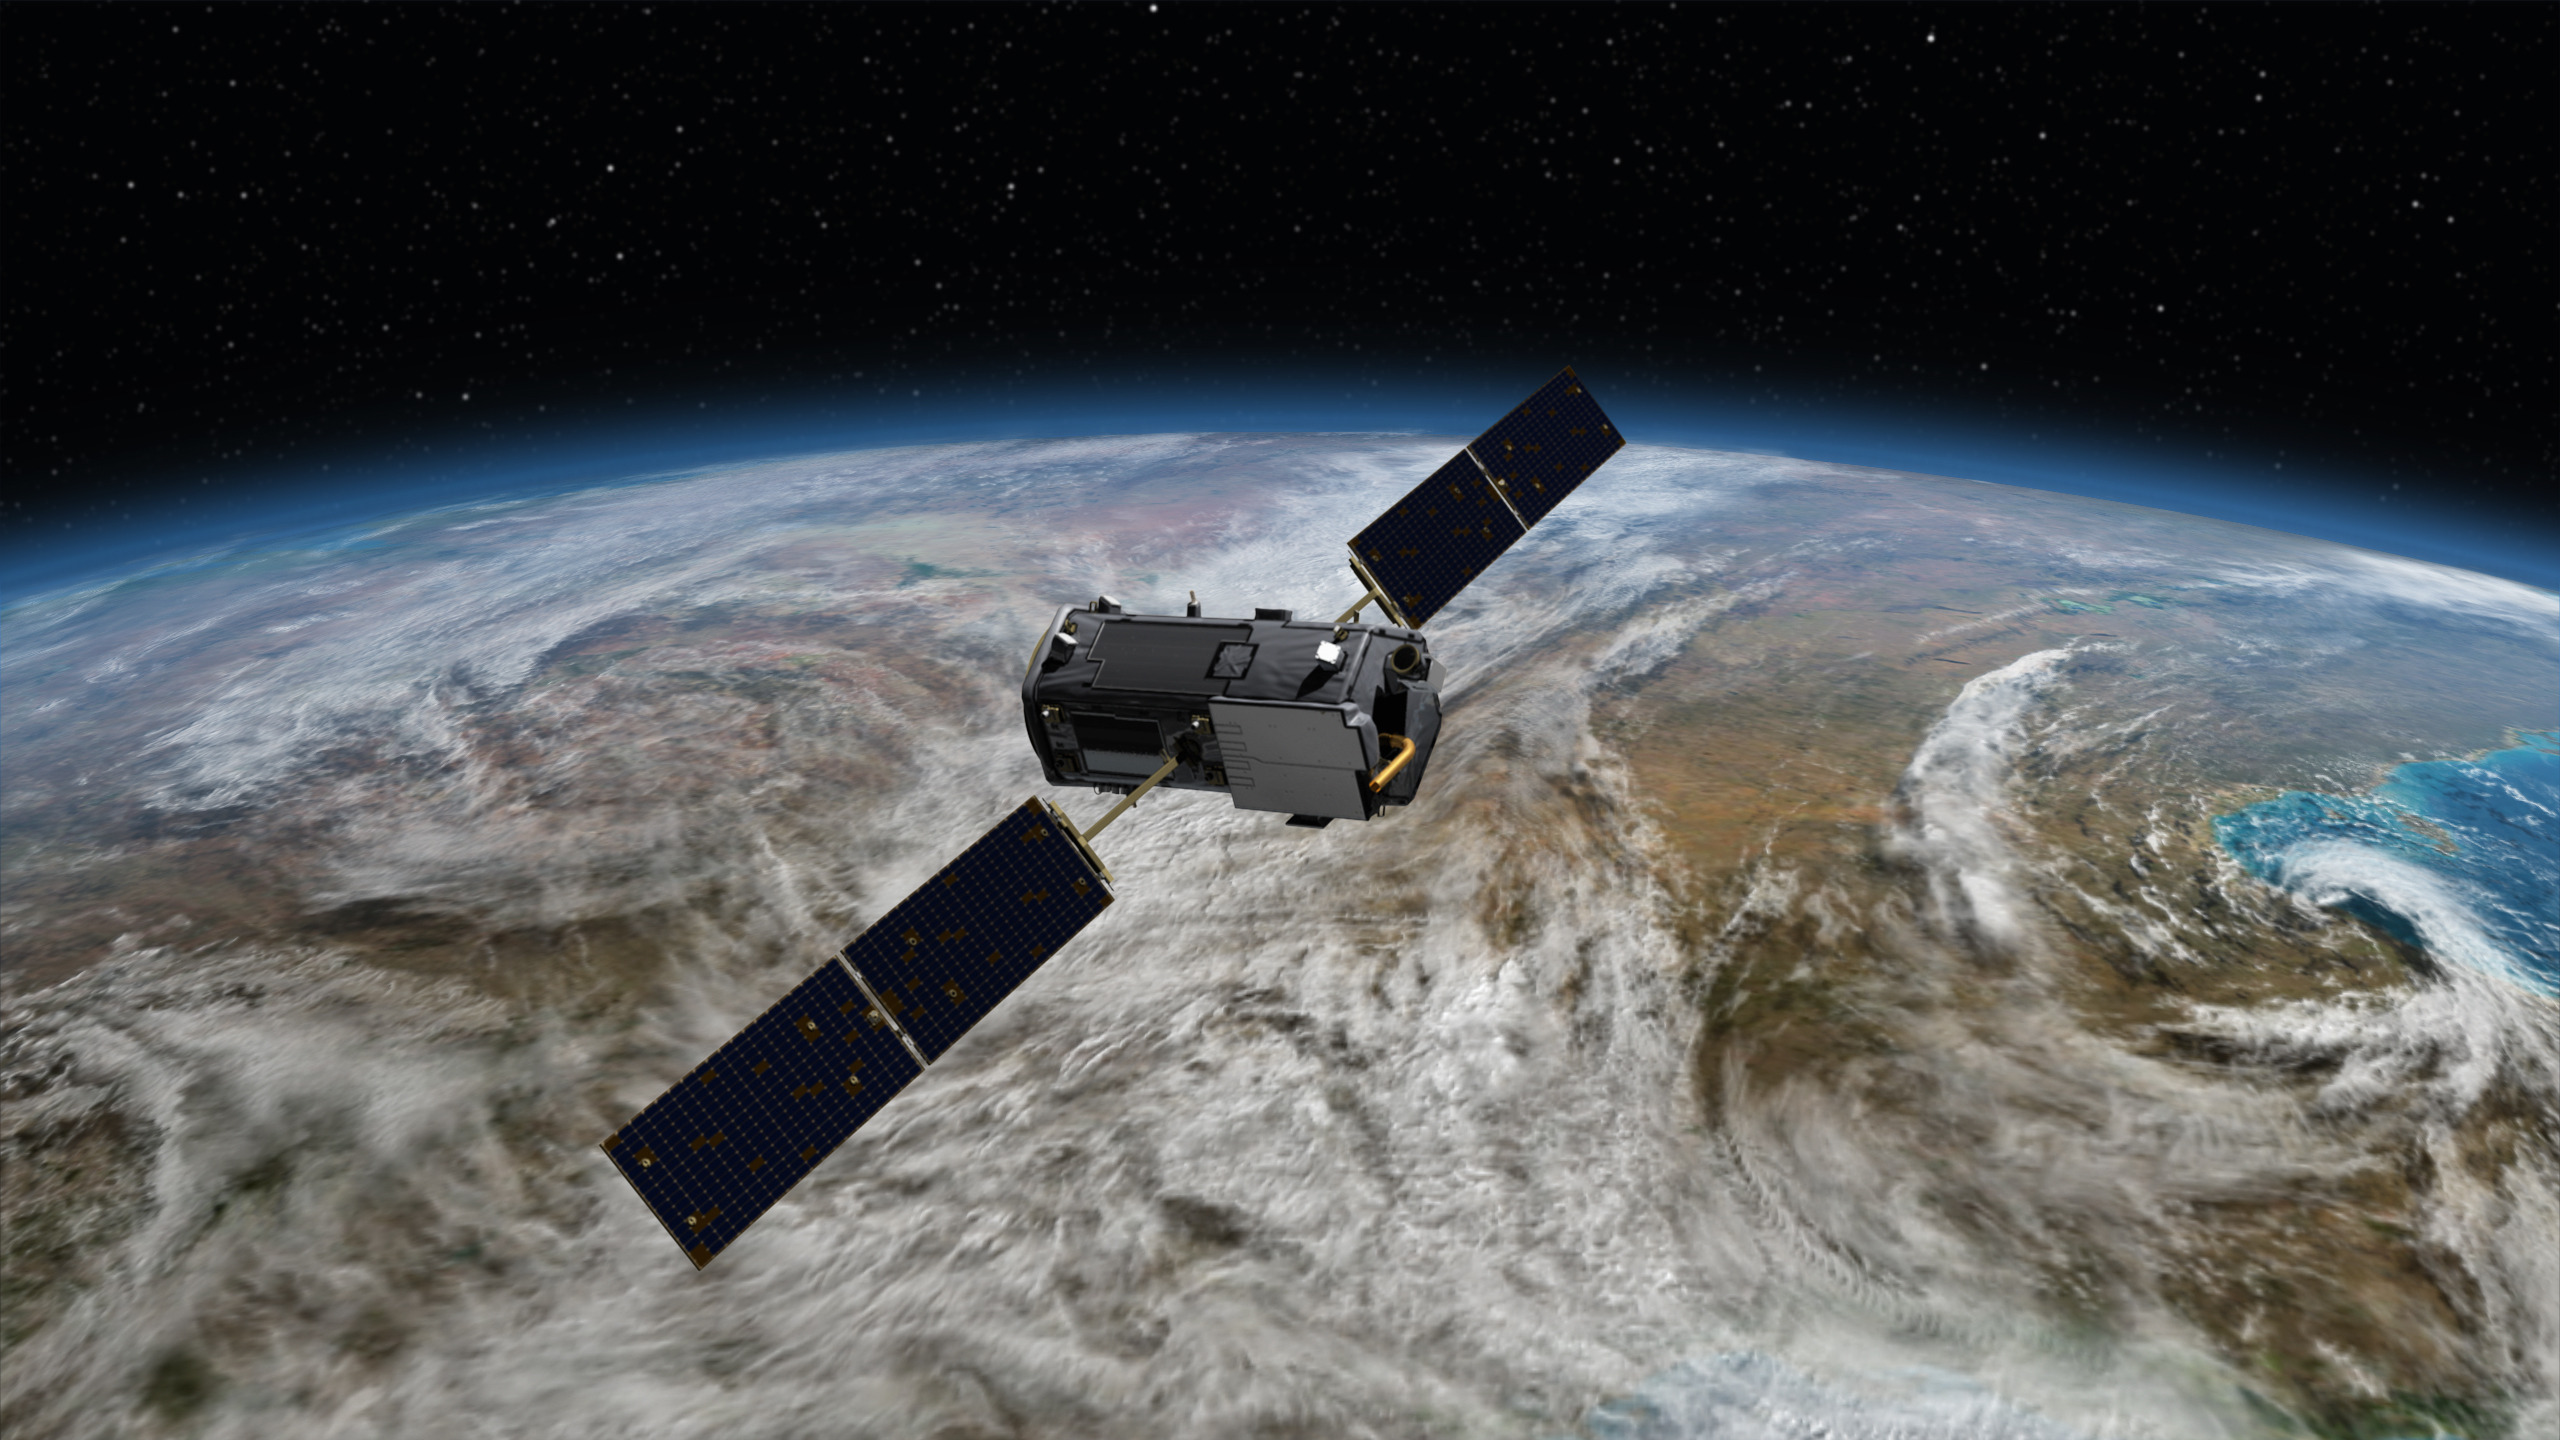
\includegraphics[width=0.9\linewidth]{2.Misiones_Semejantes/OCO2.jpg}
    \caption{Representación artística del \textit{Orbiting Carbon Observatory }(OCO)-2 de la NASA. \\Fuente: \cite{nasa_jpl_oco2_artist_concept_2014}.
}
\end{figure}

OCO-2 representa una de las misiones más significativas dedicadas exclusivamente al monitoreo de CO\textsubscript{2} atmosférico. Lanzado en julio de 2014 por la NASA, este satélite se diseñó para proporcionar mediciones precisas de la concentración de CO\textsubscript{2} a escala global, ofreciendo datos cruciales para la comprensión del ciclo del carbono terrestre.

El satélite emplea tres espectrómetros de rejilla que operan en bandas espectrales del infrarrojo cercano: 0,76 \textmu m (banda O\textsubscript{2} A), 1,61 \textmu m y 2,06 \textmu m (bandas de absorción de CO\textsubscript{2}). Los detectores utilizados son matrices de fotodiodos de silicio HAWAII-1RG fabricados por Teledyne y  mantenidos a -120 °C mediante un sistema criogénico para minimizar el ruido térmico.

El telescopio presenta un diseño Cassegrain con una apertura de 11 cm de diámetro. La resolución espacial alcanza 1,3×2,3 km con un ancho de barrido de 10 km. El satélite orbita a 705 km de altitud en una órbita heliosíncrona con inclinación de 98,2°, proporcionando un período de revisita de 16 días. La masa total del sistema es de 449 kg \cite{eoportal_oco2_2024}.

\section{GOSAT / GOSAT-2 (\textit{Greenhouse Gases Observing Satellite})}

\begin{figure}[H]
    \centering
    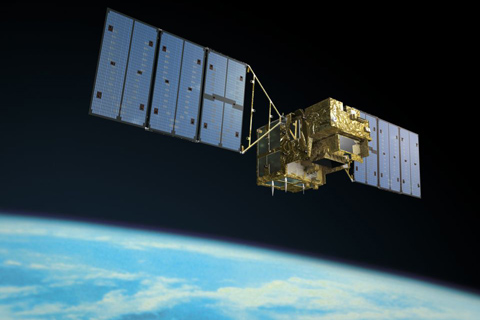
\includegraphics[width=0.8\linewidth]{2.Misiones_Semejantes/gosat_main_001.jpg}
    \caption{Representación artística de GOSAT. \\Fuente: \cite{jaxa_gosat_representation}.
}
\end{figure}

El sistema GOSAT, desarrollado por JAXA, utiliza el espectrómetro de transformada de Fourier TANSO-FTS, GOSAT-1 incorpora las siguientes bandas: Banda 1 (0,758-0,775 \textmu m) centrada en la banda de absorción del oxígeno A, Banda 2 (1,56-1,72 \textmu m) optimizada para la detección de CO\textsubscript{2} y CH\textsubscript{4}, Banda 3 (1,92-2,08 \textmu m) diseñada para CO\textsubscript{2} y H\textsubscript{2}O, y Banda 4 (5,56-14,3 \textmu m) que abarca el infrarrojo térmico para CO\textsubscript{2} y CH\textsubscript{2}. Los detectores empleados incluyen tecnología de silicio (Si) para la banda 1, InGaAs para las bandas 2 y 3, y PC-MCT (\textit{Mercury Cadmium Telluride}) para la banda 4 en el infrarrojo térmico. El telescopio presenta una apertura de 68 mm de diámetro.

La resolución espacial nominal es de 10,5 km en nadir. GOSAT-2, la versión mejorada lanzada en octubre de 2018, opera a 613 km de altitud en órbita heliosíncrona con inclinación de 98,1°, ofreciendo un período de revisita de 6 días. La masa del sistema alcanza aproximadamente 1.700 kg (masa seca), con una masa total inferior a 2.000 kg.

GOSAT-2 incorpora mejoras significativas respecto a su predecesor, incluyendo cinco bandas espectrales (en lugar de cuatro) con rangos optimizados, capacidad para medir monóxido de carbono (CO) adicional al CO\textsubscript{2} y CH\textsubscript{4}, y un mecanismo de apuntamiento inteligente para evitar nubes \cite{jaxa_gosat} \cite{gogoi2023gosat}.

\section{CO2M (\textit{Carbon Dioxide Monitoring Mission})}

\begin{figure}[H]
    \centering
    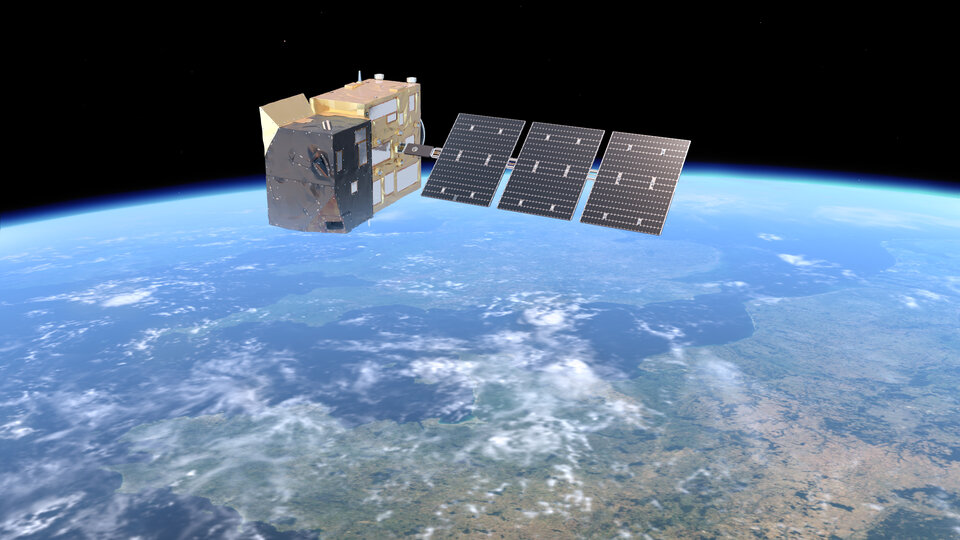
\includegraphics[width=0.8\linewidth]{2.Misiones_Semejantes/Copernicus_Carbon_Dioxide_Monitoring_mission_article-2326145821.jpg}
    \caption{CO2M, de la Agencia Espacial Europea. \\Fuente: \cite{CO2M}.
}
\end{figure}

CO2M representa una iniciativa pionera de la Agencia Espacial Europea (ESA) dentro del programa Copernicus, diseñada específicamente para monitorizar las emisiones antropogénicas de CO\textsubscript{2} a escala global. Programada para lanzarse a partir de 2025, esta misión constará de una constelación de tres satélites (CO2M-A, CO2M-B y CO2M-C) que trabajarán en conjunto para proporcionar una cobertura temporal sin precedentes.


El instrumento principal, denominado CO2I (Integrated CO\textsubscript{2} and NO\textsubscript{2} Imaging Spectrometer), es un espectrómetro de alta precisión que opera en múltiples bandas espectrales: 405-490 nm (visible), 747-773 nm (infrarrojo cercano) y dos rangos de infrarrojo de onda corta (1,59-1,67 \textmu m y 1,98-2,08 \textmu m). Los detectores utilizados son de tecnología MCT (\textit{Mercury Cadmium Telluride}). Con una resolución espacial de 4 km\textsuperscript{2}, el sistema está optimizado para identificar fuentes puntuales como centrales eléctricas y complejos industriales.


Una característica distintiva de CO2M es su sistema integrado de corrección atmosférica, que combina el instrumento CLIM (imagen de nubes en tres bandas) y el MAP (polarímetro multiangular) para filtrar datos afectados por cubierta nubosa. La constelación completa logrará una revisita global cada 3,5 días, útil para el monitoreo efectivo de áreas urbanas dinámicas, con una masa aproximada de 900 kg por satélite \cite{CO2M} \cite{CO2M_progress}.

\section{TanSat (\textit{Chinese Carbon Dioxide Observation Satellite})}

\begin{figure}[H]
    \centering
    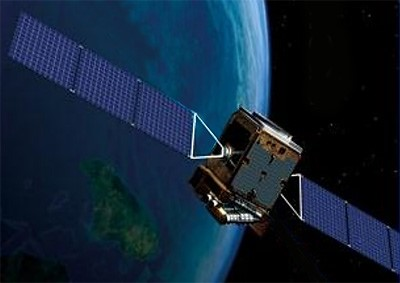
\includegraphics[width=0.8\linewidth]{2.Misiones_Semejantes/tansat.jpg}
    \caption{TanSat. \\Fuente: \cite{tansat}.
}
\end{figure}

TanSat, lanzado en diciembre de 2016 por la Academia China de Ciencias, se convirtió en el primer satélite chino dedicado específicamente a la monitorización de CO\textsubscript{2}. Su objetivo principal es medir la concentración de dióxido de carbono en la atmósfera con alta precisión y contribuir a la comprensión del ciclo global del carbono.

TanSat incorpora dos instrumentos principales: un espectrómetro de CO\textsubscript{2} de alta resolución (CarbonSpec) que opera en las bandas de 0,76 \textmu m (banda de oxígeno A), 1,61 \textmu m y 2,06 \textmu m (bandas de CO\textsubscript{2}), y un polarímetro de nube y aerosol (CAPI) que observa en siete bandas espectrales desde el ultravioleta hasta el infrarrojo cercano. Los detectores utilizados son matrices de fotodiodos de InGaAs (Indio, Galio, Arsénico) para las bandas de CO\textsubscript{2}.

El telescopio utiliza un diseño óptico tipo Offner que proporciona una resolución espacial de 2 km × 2 km con un ancho de barrido de 20 km. Este satélite orbita a una altitud de aproximadamente 700 km en una órbita heliosíncrona con inclinación de 98,2°, similar a la de OCO-2. Su masa total es de aproximadamente 620 kg \cite{eoportal_tansat}.

\section{MicroCarb (\textit{Microsatellite for Carbon Observation})}

\begin{figure}[H]
    \centering
    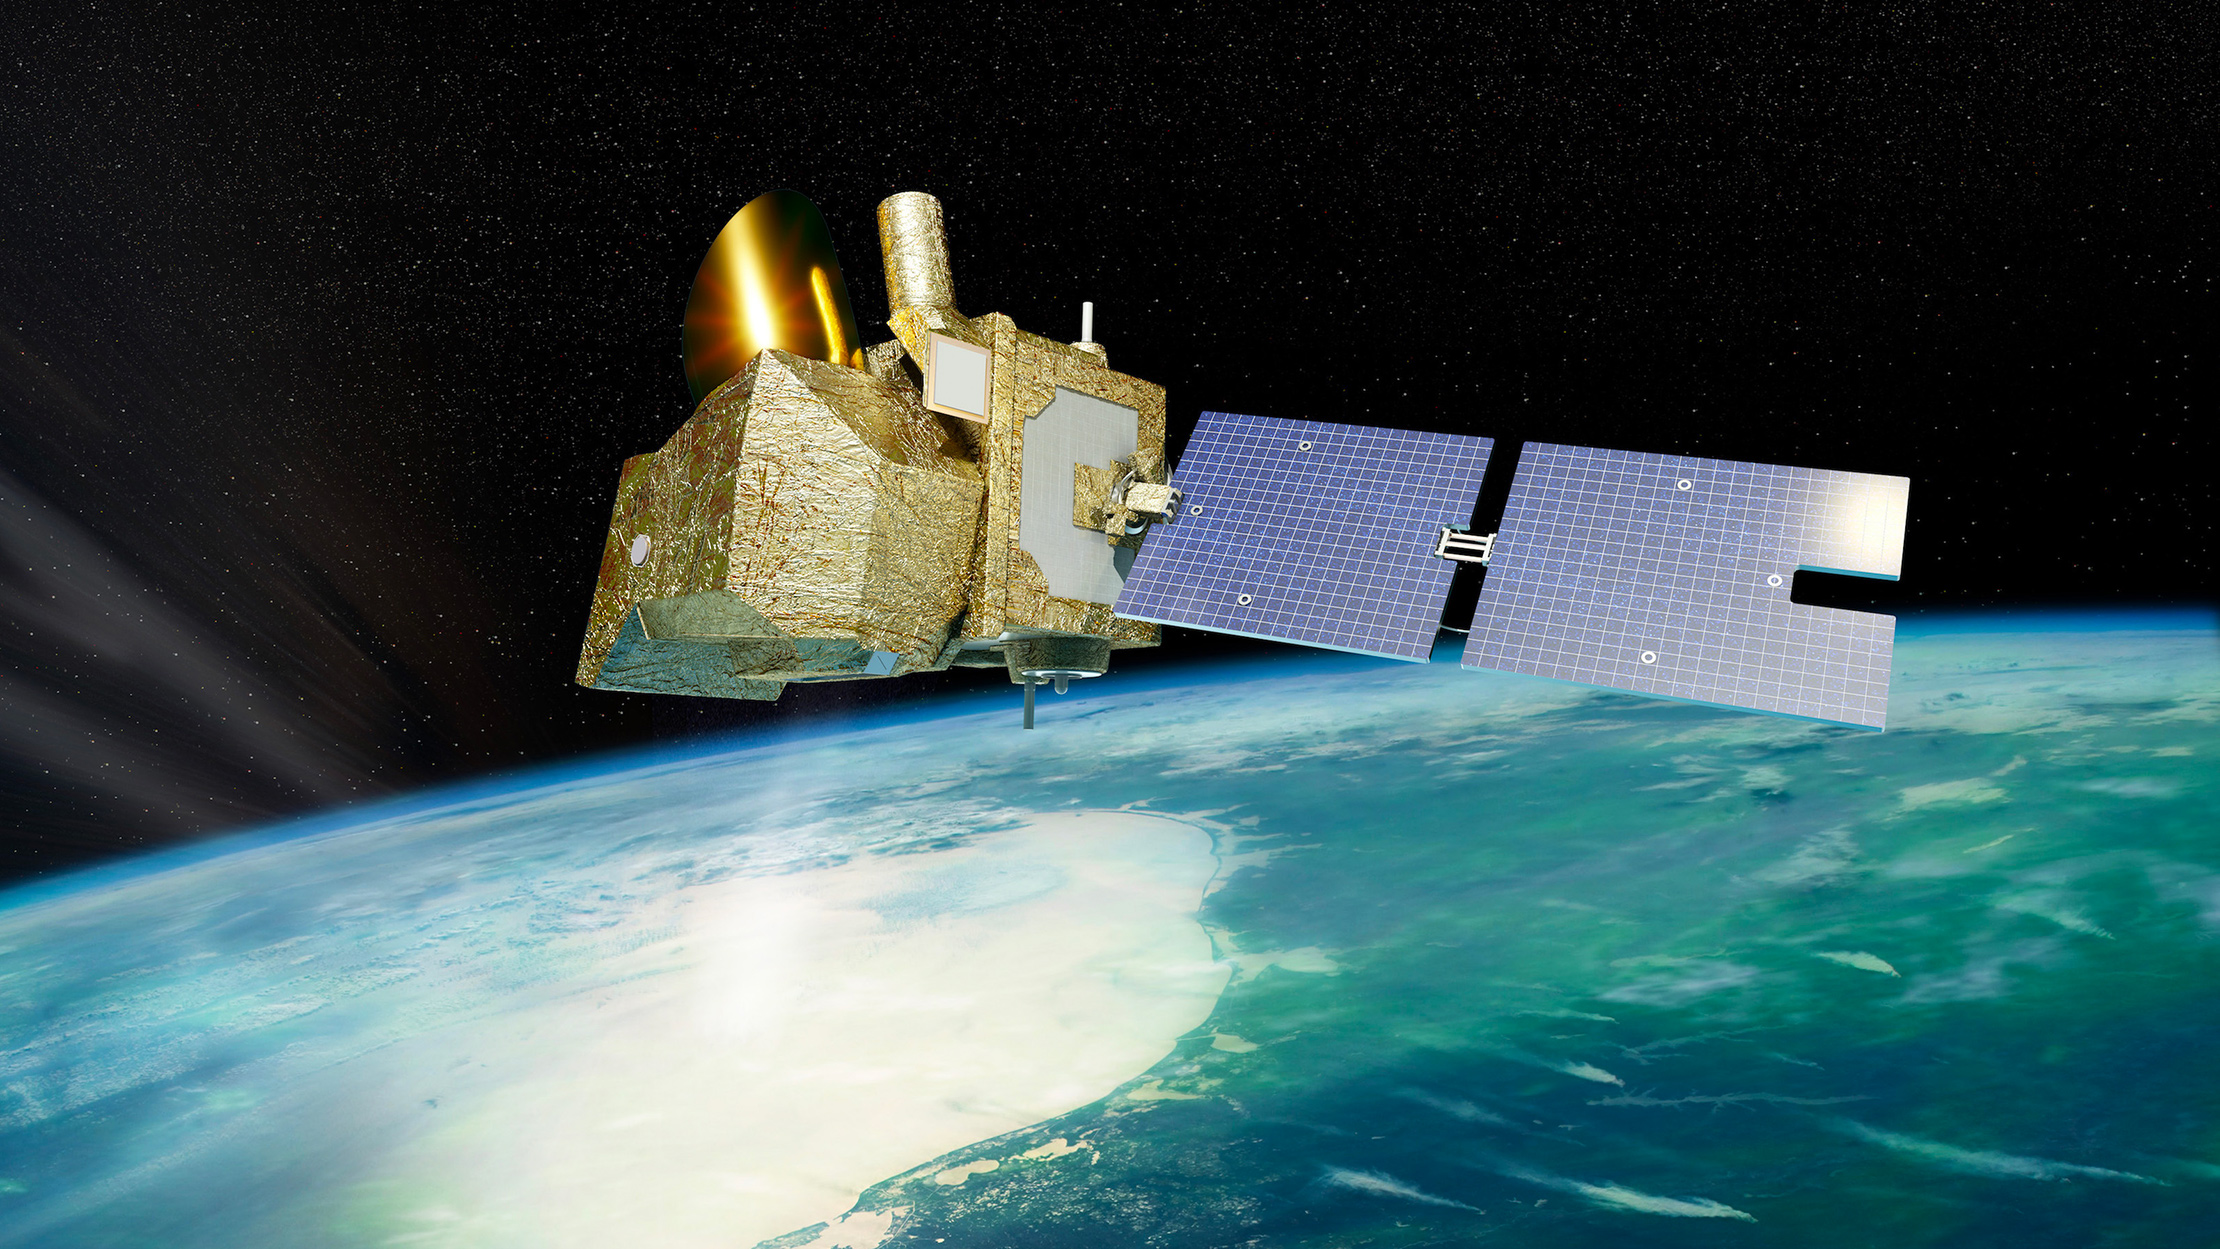
\includegraphics[width=0.8\linewidth]{2.Misiones_Semejantes/Microcarb_Airbus_Cnes_OliverSattler-1386146461.jpg}
    \caption{Imagen artistica de Microcarb. \\Fuente: \cite{futura_microcarb}
}
\end{figure}

MicroCarb es una misión desarrollada por la agencia espacial francesa CNES, con lanzamiento previsto en 2025. Representa un enfoque innovador al utilizar una plataforma de microsatélite para realizar mediciones precisas de CO$_\textsubscript{2}$ atmosférico, demostrando que misiones efectivas pueden implementarse con presupuestos y masas reducidas.

El instrumento principal de MicroCarb es un espectrómetro de rejilla compacto que opera en cuatro bandas espectrales: 0.76 \textmu m (O\textsubscript{2}), 1.27 \textmu m (O\textsubscript{2}), 1.6 \textmu m (CO\textsubscript{2}) y 2.01 \textmu m (CO\textsubscript{2}). Esta configuración permite mediciones precisas de concentración de CO\textsubscript{2} con una resolución espacial aproximada de 4.5 km × 9 km. Permite además alcanzar una resolución máxima de 2 km × 2 km en modo de escaneo urbano. 

MicroCarb operará en una órbita heliosíncrona a aproximadamente 650 km de altitud con un período de revisita de 25 días. Lo que destaca de esta misión es su masa total de solo 180 kg, significativamente menor que otras misiones similares, demostrando los avances en la miniaturización de tecnologías espaciales \cite{eoportal_microcarb}.

\section{GHGSat}

\begin{figure}[H]
    \centering
    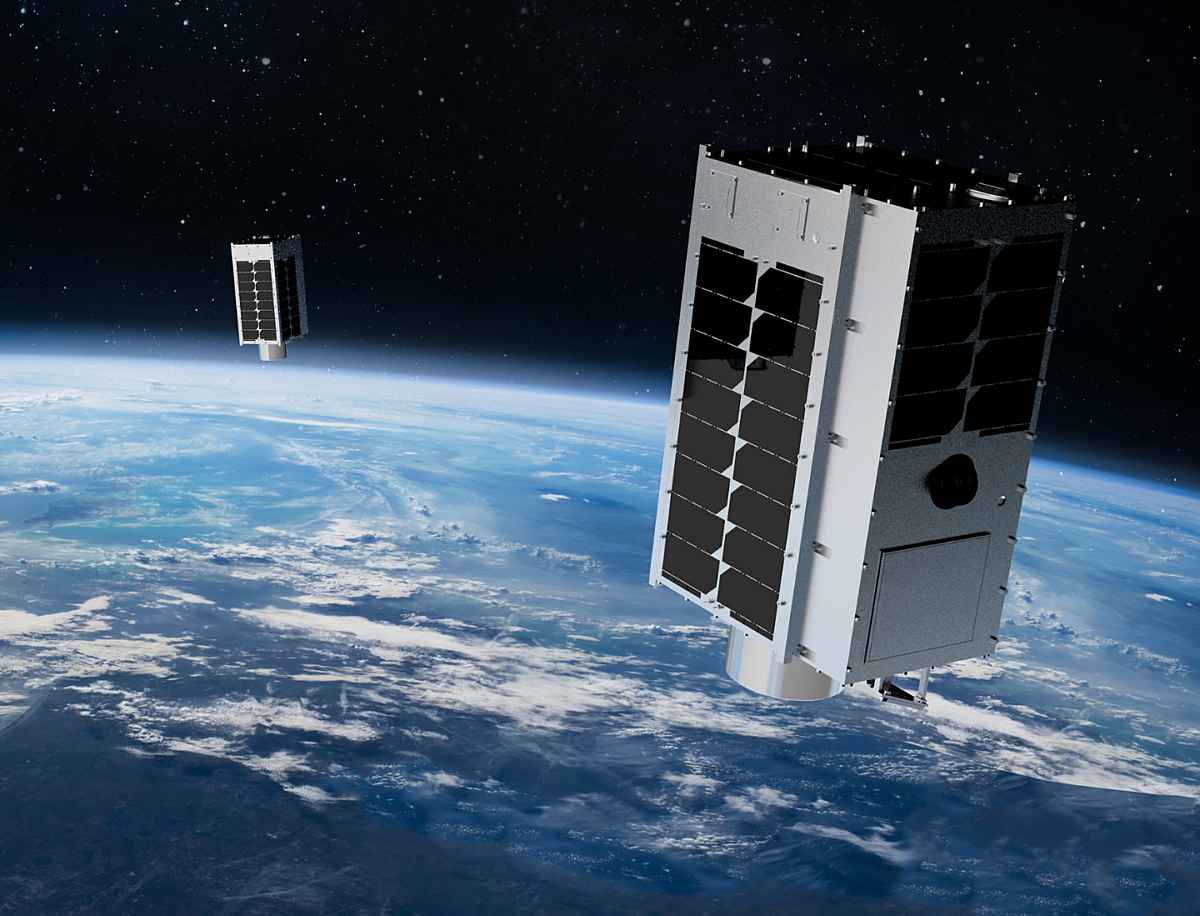
\includegraphics[width=0.8\linewidth]{2.Misiones_Semejantes/GHGSat_Constellation-of-Six-Satellites_1440x1100-2772752015.png}
    \caption{Constelacion GHGSat. \\Fuente: \cite{gosat_gw}
}
\end{figure}

La constelación GHGSat representa un enfoque comercial al monitoreo de gases de efecto invernadero. Esta constelación se dedica a la detección de emisiones de metano y CO$_\textsubscript{2}$ a nivel de instalaciones individuales, ofreciendo una resolución espacial sin precedentes para aplicaciones específicas de monitorización de fuentes puntuales.


Cada satélite GHGSat está equipado con un espectrómetro de imagen compacto denominado WAF-P (Wide-Angle Fabry-Perot) que opera en bandas del infrarrojo cercano específicas para la detección de metano y CO\textsubscript{2}. Los detectores utilizados son de tecnología InGaAs, optimizados para la detección en el rango espectral de 1600-1700 nm. El telescopio emplea un diseño reflectivo con una apertura de aproximadamente 5 cm.


La tecnología patentada permite una resolución espacial de aproximadamente 25 metros, capacitando la identificación precisa de fuentes de emisión. Los satélites GHGSat operan en órbitas heliosíncronas a altitudes entre 500-550 km con una inclinación de 97,5°. Cada unidad tiene una masa de aproximadamente 15-20 kg, ejemplificando el potencial de los nanosatélites para aplicaciones de observación terrestre especializadas \cite{wmo_ghgsat_spectrometer}.






\section{Hallazgos clave}
Primeramente se presenta una tabla comparativa con el fin de resumir las principales características de las misiones analizadas:



\begin{landscape}
\begin{table}[p]
\centering
\caption{Comparativa de misiones de observación de CO\textsubscript{2}.}
\small
\begin{tabular}{lcccccc}
\toprule
\textbf{Parámetro} & \textbf{OCO-2} & \textbf{GOSAT2} & \textbf{CO2M} & \textbf{TanSat} & \textbf{MicroCarb} & \textbf{GHGSat} \\
\midrule
Detector & Fotodiodos Si  & InSb/MCT & MCT & InGaAs & MCT & InGaAs \\
Diámetro pupila (cm) & 11 & 10 & 15 & 12 & 8 & 5 \\
GSD (km) & 1.3$\times$2.3 & 10 & 2 & 2 & 4.5 & 0.025 \\
Swath (km) & 10 & 10 & 250 & 20 & 250 & 12 \\
Altura orbital (km) & 705 & 666 & 735 & 700 & 650 & 500 \\
Tipo órbita & SSO 98.2° & SSO 98.1° & SSO 97.7° & SSO 97.4° & SSO 98.0° & SSO 97.6° \\
Constelación & No & No & Sí (3) & No & No & Sí (10+) \\
Tipo telescopio & Cassegrain & FTS & Cassegrain & Offner & Off-axis & Reflective \\
Duración (años) & 2 (+10) & 5 & 7.5 & 5 & 3 & 5 \\
Revisita (días) & 16 & 3 & 3.5 & 16 & 25 & 5 \\
Masa (kg) & 450 & 2900 & 900 & 600 & 180 & 15 \\
Paneles solares (m$^2$) & 8 & 24 & 12 & 10 & 4 & 1.8 \\
Cobertura & Global & Global & Global & Global & Global & Puntual \\
\bottomrule
\end{tabular}

\end{table}
\end{landscape}

Del análisis comparativo de las estas misiones se pueden extraer los siguientes hallazgos clave, que serán útiles para inspirar la misión encomendada:

\begin{itemize}
    \item Las misiones analizadas muestran diferentes aproximaciones al monitoreo de CO\textsubscript{2}, desde satélites individuales de gran tamaño (GOSAT-2) hasta constelaciones de microsatélites (GHGSat), pasando por soluciones intermedias como MicroCarb.
    \item Se utilizan diferentes tecnologías de detección según los requerimientos específicos de cada misión, desde fotodiodos de silicio (OCO-2) hasta detectores de InGaAs (TanSat, GHGSat) y MCT (GOSAT-2, CO2M)
    \item Las constelaciones como CO2M y GHGSat logran períodos de revisita significativamente menores (3,5 y 5 días respectivamente) que los satélites individuales, mejorando la capacidad de monitoreo temporal.
    \item La selección universal de órbitas heliosíncronas en todas las misiones analizadas demuestra su importancia crítica para la observación terrestre. Esta configuración orbital garantiza condiciones de iluminación consistentes al pasar sobre cualquier punto de la superficie terrestre a la misma hora solar local, lo que resulta fundamental para la comparabilidad temporal de los datos espectrales. Adicionalmente, la órbita heliosíncrona facilita la cobertura global sistemática con períodos de revisita predecibles, optimizando tanto la adquisición de datos como la planificación de misiones de monitoreo ambiental.

\end{itemize}
\chapter{Conceptos Previos}\label{cap3}
\minitoc

En este apartado del trabajo se van a asentar las bases teóricas y conceptos necesarios para poder, partiendo de esta base definir las necesidades de nuestra carga de pago, así como buscar la solución optima para satisfacer la solución de diseño.


\newpage


\section{Calidad de Imagen}
\subsection{\textit{Aliasing}}


\begin{figure}[H]
    \centering
    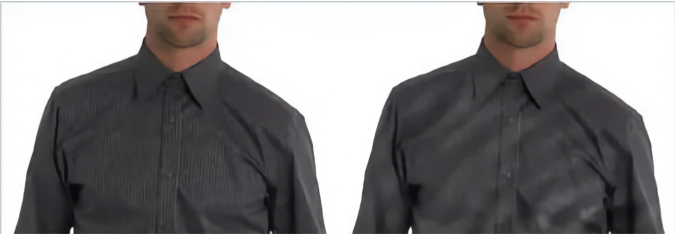
\includegraphics[width=0.7\textwidth]{3.Conceptos_Previos/Moire effect.jpg}
    \caption{Ejemplo del efecto del aliasing sobre un patrón visual.\\ Fuente: \cite{kitdeactores2025moire}}
    \label{fig:Aliasing}
\end{figure}

El \textit{aliasing} es un fenómeno que ocurre cuando una señal con componentes de alta frecuencia es muestreada a una tasa insuficiente, lo que provoca que las frecuencias originales se mezclen y aparezcan como frecuencias más bajas en el espectro reconstruido. En términos de imágenes satelitales, el \textit{aliasing} puede causar artefactos visuales o distorsiones en los datos, degradando la calidad de la imagen capturada. Este problema está directamente relacionado con la frecuencia de Nyquist, que establece que la tasa de muestreo debe ser al menos el doble de la frecuencia espacial máxima presente en la escena para evitar \textit{aliasing}.

\subsection{\textit{Ground Sampling Distance} (GSD)}

\begin{figure}[H]
    \centering
    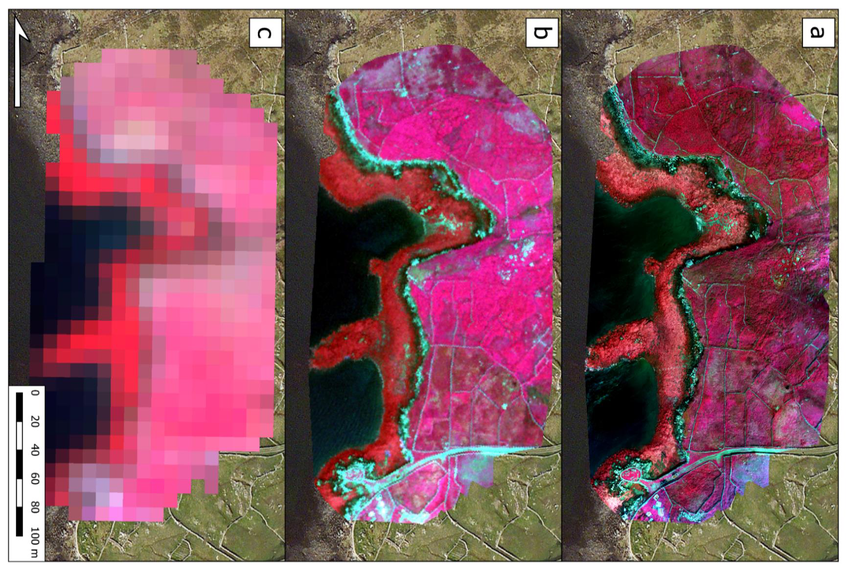
\includegraphics[width=0.7\textwidth]{3.Conceptos_Previos/Comparison-of-the-multispectral-ground-sampling-distance-GSD-from-each-of-the-three.ppm.png}
    \caption{Efectos de distintos GSD en imágenes tomadas por satélite.\\ Fuente: \cite{rossiter2020gsd_comparison}}
    \label{fig:gsdexample}
\end{figure}

La \textbf{Ground Sampling Distance (GSD)} es la distancia en terreno que corresponde a un solo píxel en la imagen capturada por el satélite, determinando la resolución espacial del sistema. Se calcula mediante la relación geométrica entre el tamaño del píxel del detector (\( p \)), la altura orbital (\( h \)) y la distancia focal del telescopio (\( f \)):
\begin{align}
\text{GSD} = \frac{p \cdot h}{f}
\end{align}


\subsection{Frecuencia de Nyquist($f_{Ny}$)}

La \textbf{frecuencia de Nyquist} es un concepto fundamental en la teoría de muestreo que define la máxima frecuencia espacial que un sistema de imagen puede capturar sin distorsión por \textit{aliasing}. En el contexto de un satélite de observación terrestre, esta frecuencia está directamente ligada a la resolución espacial (GSD) y determina la capacidad del sistema para preservar detalles finos en la escena observada.

La frecuencia de Nyquist (\( f_{\text{Nyquist}} \)) se calcula como:
s
\begin{align}
f_{\text{Nyquist}} = \frac{1}{2 \cdot p}
\end{align}

donde el \text{tamaño del pixel} actúa como el intervalo de muestreo espacial.

\subsection{\textit{Modulation Transfer Function} (MTF)}\label{sec:mtfteoria}

La Función de Transferencia de Modulación (MTF) es una herramienta matemática fundamental para evaluar la calidad óptica de un sistema de observación terrestre. La MTF mide la capacidad del sistema óptico para reproducir el contraste de la imagen en función de la frecuencia espacial \cite{design_workshop_optical_2023} \cite{zorita_mtf_2023}.

\begin{figure}[H]
    \centering
    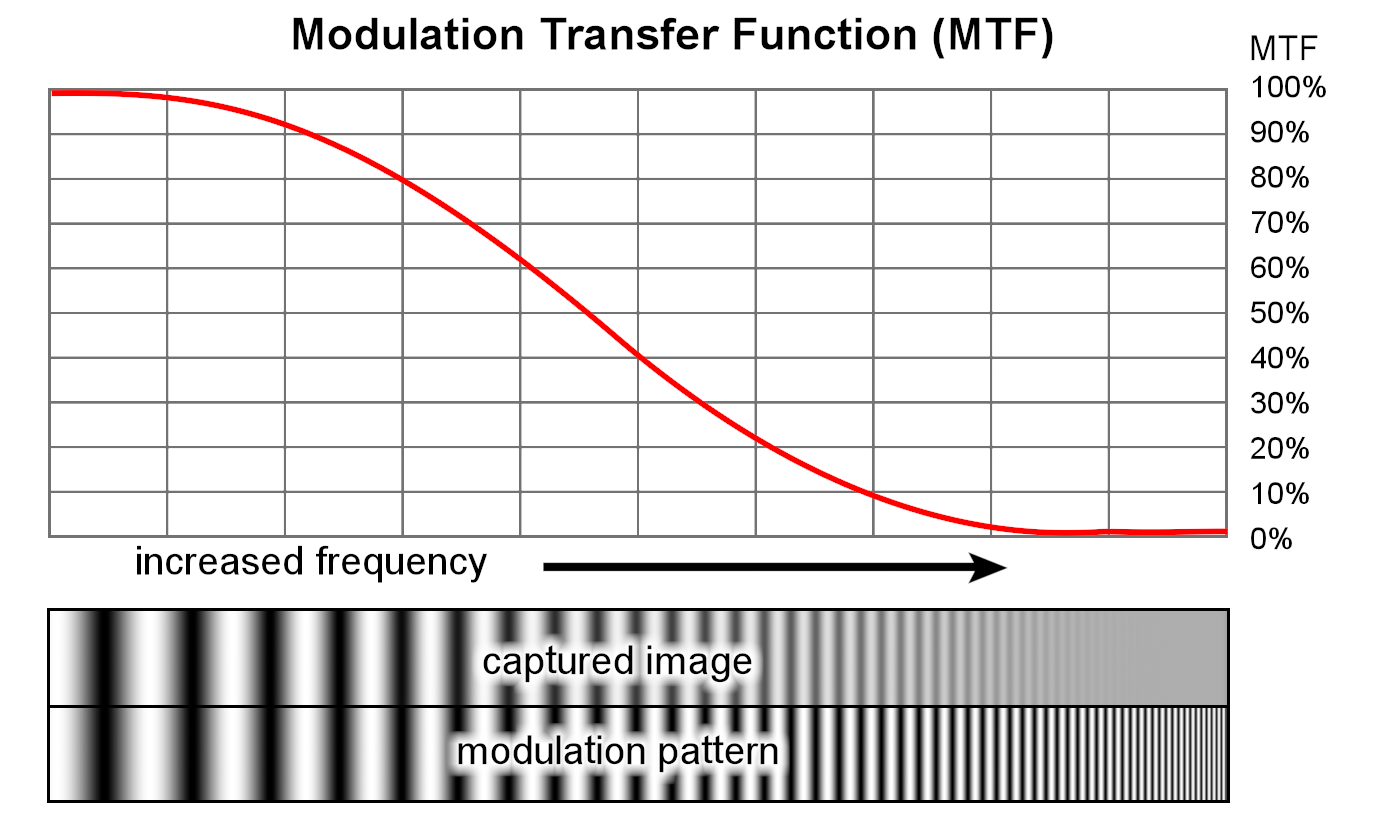
\includegraphics[width=0.7\textwidth]{3.Conceptos_Previos/MTF.png}
    \caption{Representación visual de la MTF.\\ Fuente: \cite{EdmundOptics2023}.}
    \label{fig:MTF}
\end{figure}

En términos simples, la MTF determina cómo un sistema óptico transfiere el contraste desde el objeto hasta la imagen final. Cuando se observa un patrón de franjas blancas y negras (alto contraste), la MTF indica qué porcentaje de ese contraste se preserva en la imagen final. A medida que aumenta la frecuencia espacial (franjas más densas), el contraste tiende a disminuir.


La MTF total del sistema es el producto de las MTF de cada uno de los subsistemas ópticos y electrónicos relevantes. Los principales contribuyentes son:

\begin{itemize}
  \item \textbf{MTF de Difracción:} Limitación física impuesta por el diámetro de la apertura del telescopio y la longitud de onda de observación. Para una apertura circular sin obstrucción, la MTF de difracción se calcula mediante:

  \begin{equation}
  MTF_{\text{difracción}}(f_x) = \frac{2}{\pi} \left[ \arccos\left(\frac{f_x}{f_{co}}\right) - \frac{f_x}{f_{co}} \sqrt{1 - \left(\frac{f_x}{f_{co}}\right)^2} \right]
  \end{equation}

  donde $f_{co} = D / \lambda$ es la frecuencia de corte, $D$ el diámetro de la apertura y $\lambda$ la longitud de onda.

  Para un telescopio obscurado\footnote{obstrucción central que bloquea parte de la luz (normalmente un espejo) que entra al sistema óptico, siendo $d_{obs}$ la medida de dicha obstrucción}, como es el caso de los telescopios Cassegrain y Korsch, su MTF de difracción vendrá definida, en función del diámetro de obscuración $d_{obs}$. Para el presente trabajo se establecerá $R_{obs} = 0,2$ como valor inicial.\cite{Foadi2023DesigningCT}
\begin{equation}
\mathrm{OTF}_{\mathrm{diff}} = \frac{A + B + C}{1 - R^2}
\end{equation}

\begin{equation}\label{mtfrobs}
R = \frac{d_{\mathrm{obs}}}{D_o}
\end{equation}

\begin{equation}
X = \frac{f_x}{f_{\mathrm{oco}}}, \quad Y = \frac{X}{R}, \quad \alpha = \cos^{-1}\left(\frac{1 + R^2 - 4X^2}{2R}\right)
\end{equation}

\begin{equation}
A =
\begin{cases}
\frac{2}{\pi}\left[\cos^{-1}(X) - X\sqrt{1 - X^2}\right], & \text{si } 0 \leq X \leq 1 \\
0, & \text{en otro caso}
\end{cases}
\end{equation}

\begin{equation}
B =
\begin{cases}
\frac{2R^2}{\pi}\left[\cos^{-1}(Y) - Y\sqrt{1 - Y^2}\right], & \text{si } 0 \leq Y \leq 1 \\
0, & \text{en otro caso}
\end{cases}
\end{equation}

\begin{equation}
C =
\begin{cases}
-2R^2, & \text{si } 0 < X \leq \frac{1 - R}{2} \\
\frac{2R}{\pi} \sin\alpha + \frac{1 + R^2}{\pi} \alpha - \frac{2(1 - R^2)}{\pi} \tan^{-1}\left[\left(\frac{1 + R}{1 - R}\right)\tan\left(\frac{\alpha}{2}\right)\right] - 2R^2, & \text{si } \frac{1 - R}{2} < X < \frac{1 + R}{2} \\
0, & \text{si } X \geq \frac{1 + R}{2}
\end{cases}
\end{equation}

Para calcular el requerimiento de MTF, se impone $f_x=f_{Ny}*f$. 
  \item \textbf{MTF de Aberraciones:} Degradación adicional debida a imperfecciones ópticas (aberraciones esféricas, cromáticas, etc.). Un valor típico para sistemas bien diseñados es $MTF_{\text{aberraciones}} \approx 0{,}95$.

  \item \textbf{MTF de Fabricación:} Defectos en la fabricación de los espejos/lentes, típicamente $MTF_{\text{fabricación}} \approx 0{,}98$.

  \item \textbf{MTF de Alineamiento:} Errores en el alineamiento de los elementos ópticos. El valor depende del tipo de telescopio.

  \item \textbf{MTF por Vibraciones y Termoelasticidad:} Cambios entre el alineamiento en tierra y en órbita (vibraciones del lanzamiento y efectos térmicos), típicamente $\approx 0{,}99$ y $\approx 0{,}95$ respectivamente.

  \item \textbf{MTF del Detector:} Es un parámetro definido por el diseño y tecnología del detector, normalmente proporcionado por el fabricante.
  
\end{itemize}
Por tanto, la MTF del sistema será:

\begin{align}
MTF_{\text{sistema}} =\ & MTF_{\text{difracción}} \times MTF_{\text{aberraciones}} \times MTF_{\text{fabricación}} \times MTF_{\text{alineamiento}} \nonumber \\
& \times MTF_{\text{vibraciones}} \times MTF_{\text{termoelástico}} \times MTF_{\text{detector}}
\end{align}


\subsection{\textit{Signal To Noise Ratio} (SNR)}\label{snr}
\begin{figure}[H]
    \centering
    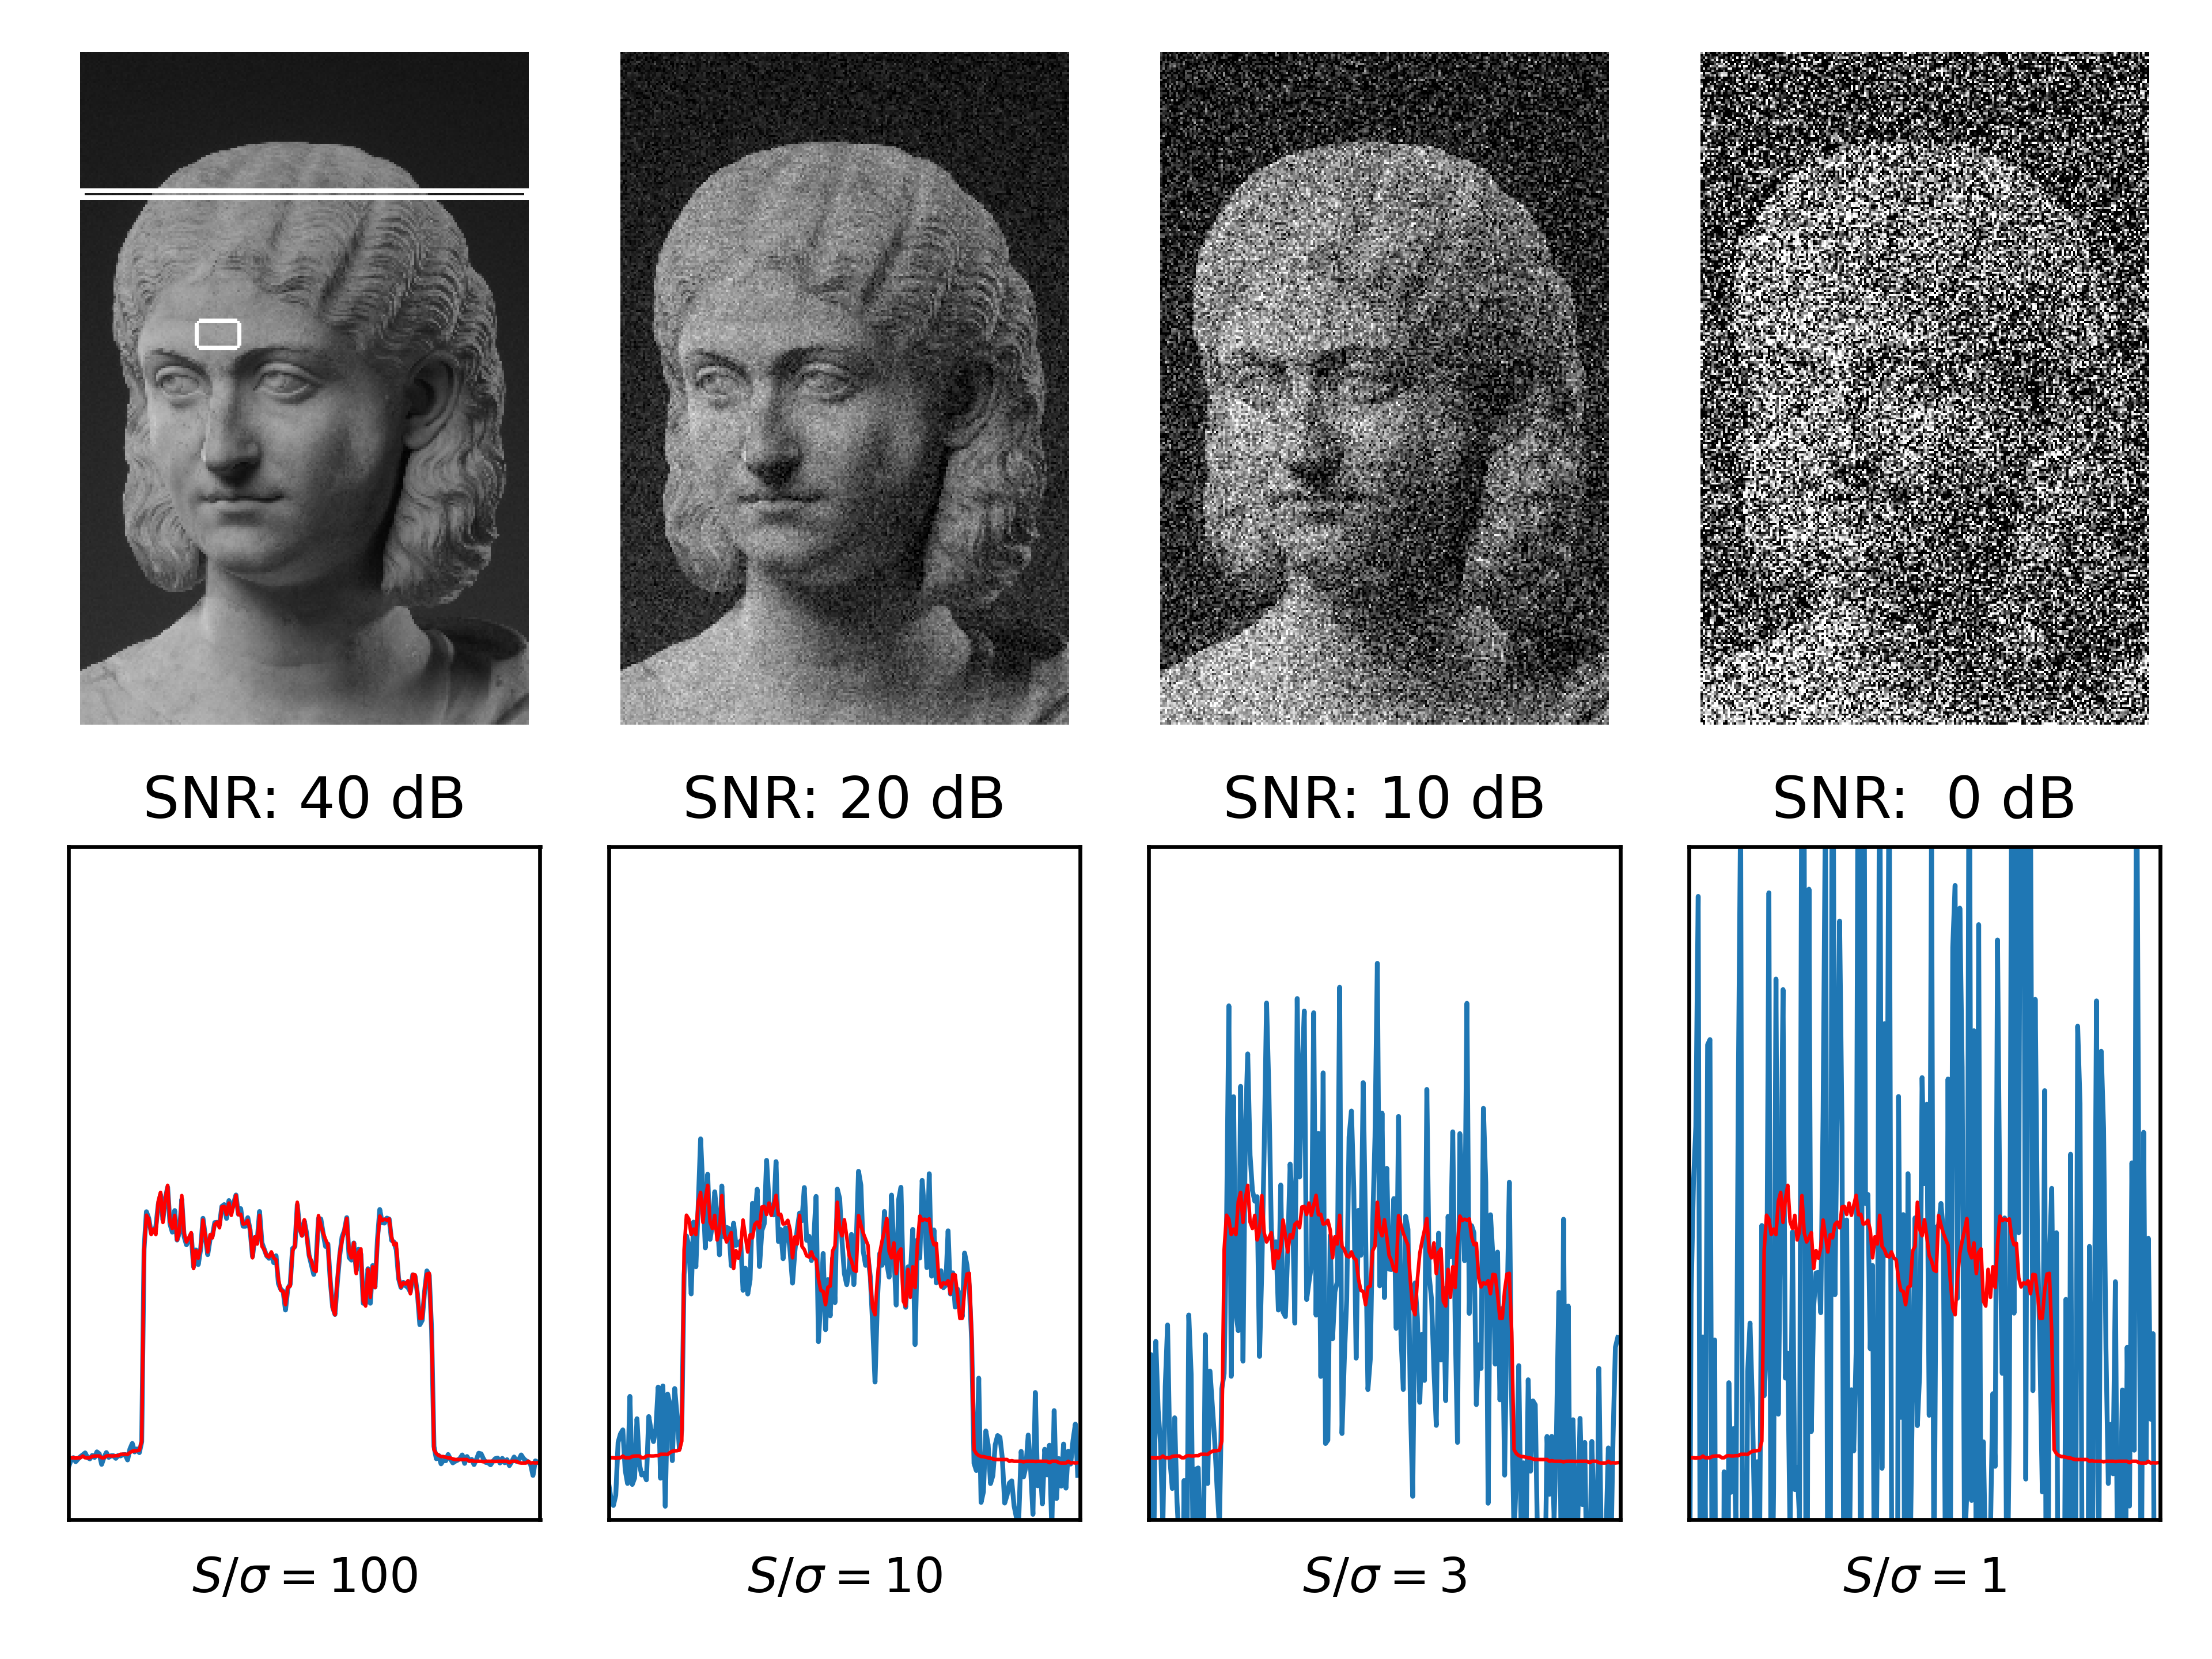
\includegraphics[width=0.5\linewidth]{3.Conceptos_Previos/SNR_image_demonstration.png}
    \caption{Efecto de la SNR.\\ Fuente: \cite{wikipedia2025snr_demonstration}}
    \label{fig:snr}
\end{figure}

La \textit{Signal-to-Noise Ratio} (SNR, o relación señal-ruido) es una métrica clave que indica la calidad radiométrica de un sistema de observación óptica. Representa la relación entre la señal útil (fotones detectados provenientes de la escena) y el ruido total (sumatoria de todas las fuentes de ruido del sistema) en el detector. Un SNR alto significa que la señal es claramente distinguible del ruido, lo que permite obtener imágenes precisas y fiables; un SNR bajo implica que la señal está enmascarada por el ruido, dificultando la detección de detalles y la calidad de los datos obtenidos\cite{design_workshop_optical_2023}\cite{zorita_snr_2023}.

Matemáticamente se expresa como:

\begin{equation}
SNR = \frac{\text{Señal}}{\text{Ruido total}}
\end{equation}

donde la señal y el ruido se expresan en número de electrones generados ($e^-$)en el detector durante el tiempo de integración.

\subsubsection{Cálculo de la Señal}


Se considera una radiancia de referencia \( L_{\mathrm{ref}} \) expresada en \( \si{\watt\per\metre\squared\per\steradian\per\micro\metre} \), centrada en una longitud de onda \( \lambda_c \) con un ancho de banda espectral \( \Delta \lambda \). La radiancia incidente se transmite a través del sistema óptico con una eficiencia total condicionada por la transmisión óptica del telescopio \( \tau \) y la eficiencia cuántica del detector \( \eta \). 

La irradiancia \( I \) en el plano focal se estima mediante:

\begin{equation}
I = \frac{\pi \cdot \tau \cdot \Delta \lambda \cdot L_{\mathrm{ref}}}{1 + 4F\#}
\end{equation}

donde \( F\# = \frac{f}{D} \) es la relación focal del sistema, con \( f \) la distancia focal y \( D \) el diámetro de la apertura.\footnote{Para los sistemas obscurados se utilizará la relación focal equivalente $T\#$, definida mas adelante en la ecuación \ref{relfoc}}.

La cantidad de electrones generados por píxel durante el tiempo de integración se calcula como:

\begin{equation}
N_e = \frac{E \cdot A_p \cdot \eta \cdot \lambda_c \cdot TDI \cdot t_{\mathrm{int}}}{h \cdot c}
\end{equation}

donde:
\begin{itemize}
    \item \( A_p = d_x \cdot d_y \) es el área de un píxel en el detector.
    \item \( TDI \) es el número de etapas del sistema Time Delay Integration.\footnote{Dicho concepto se explicará mas adelante en \ref{sec:tdi}}.
    \item \( t_{\mathrm{int}} = \frac{\mathrm{GSD}}{v_{\mathrm{orb}}} \) es el tiempo de integración basado en la velocidad del satélite sobre el suelo.
    \item \( h \) es la constante de Planck.
    \item \( c \) es la velocidad de la luz.
\end{itemize}

El tiempo de integración \( t_{\mathrm{int}} \) representa la duración durante la cual la imagen de un punto en la superficie terrestre permanece proyectada sobre un mismo píxel del detector mientras el satélite avanza en su órbita. Este tiempo depende directamente de la \textit{Ground Sampling Distance} (GSD) y de la velocidad del satélite sobre el suelo \( v_{\mathrm{orb}} \). Se calcula como:

\begin{equation}
t_{\mathrm{int}} = \frac{\mathrm{GSD}}{v_{\mathrm{orb}}}
\end{equation}

La velocidad orbital del satélite a una altitud \( H\) se estima aplicando la tercera ley de Kepler:

\begin{equation}
v_{\mathrm{orb}} = \sqrt{\frac{\mu}{R_T + H}}
\end{equation}

donde \( \mu = 3.986 \times 10^{14} \, \si{m^3/s^2} \) es el parámetro gravitacional estándar de la Tierra y \( R_T = 6371 \, \si{km} \) es el radio medio terrestre. Este tiempo de integración se utiliza directamente en el cálculo de \( N_e \), y representa el tiempo efectivo durante el cual se acumulan fotones en cada píxel del detector.

\subsubsection{Cálculo del Ruido Total}

El ruido total es la raíz cuadrada de la suma de las varianzas de todas las fuentes de ruido independientes del sistema, expresadas en número de electrones:

\begin{equation}
\text{Ruido total} = \sqrt{\sigma_{\text{fotónico}}^2 + \sigma_{\text{stray}}^2 + \sigma_{\text{dark}}^2 + \sigma_{\text{lectura}}^2 + \sigma_{\text{amp}}^2 + \sigma_{\text{vídeo}}^2 + \sigma_{\text{jitter}}^2 + \sigma_{\text{EMC}}^2 + \sigma_{\text{cuant}}^2}
\end{equation}

Las principales fuentes de ruido son:

\begin{itemize}
    \item \textbf{Ruido fotónico (shot noise):} Raíz cuadrada del número de electrones generados por la señal, debido a la naturaleza estadística de la llegada de fotones (\( \sqrt{N_{e^-}} \)).
    \item \textbf{Ruido de corriente de oscuridad:} Asociado a electrones generados térmicamente en el detector, incluso en ausencia de luz.
    \item \textbf{Ruido de lectura:} Introducido por la electrónica de lectura del detector.
    \item \textbf{Otros ruidos electrónicos:} Como preamplificadores, cadena de vídeo, jitter, EMC, etc.
    \item \textbf{Ruido de cuantificación:} Introducido al digitalizar la señal.
\end{itemize}

\subsubsection{Expresión Final de la SNR}

Realizando el cociente entre señal y ruido, resulta la ecuación:

\begin{equation}
SNR = \frac{N_{e^-}}{\sqrt{N_{e^-} + \sigma_{\text{stray}}^2 + \sigma_{\text{dark}}^2 + \sigma_{\text{lectura}}^2 + \sigma_{\text{amp}}^2 + \sigma_{\text{vídeo}}^2 + \sigma_{\text{jitter}}^2 + \sigma_{\text{EMC}}^2 + \sigma_{\text{cuant}}^2}}
\end{equation}


\subsection{\textit{Field of View} (FoV). \textit{Swath}}

\begin{figure}[H]
    \centering
    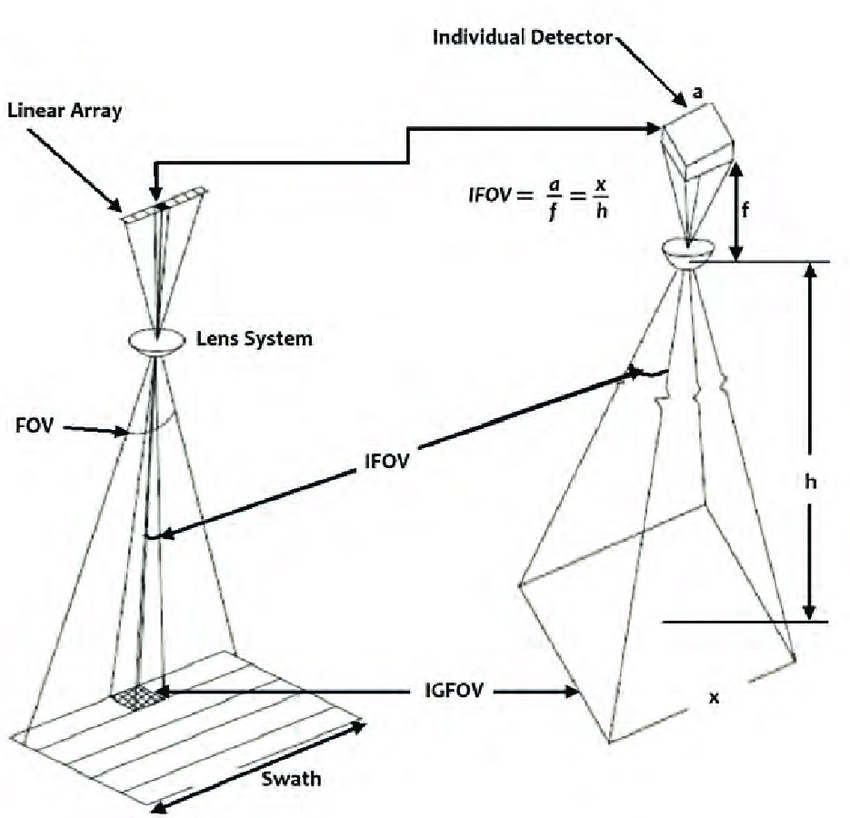
\includegraphics[width=0.7\textwidth]{3.Conceptos_Previos/Swath,fov.png}
    \caption{Esquema visual del \textit{swath} y FoV.\\Fuente: \cite{swath_fov_diagram}.}
    \label{fig:swath}
\end{figure}

El \textit{\textbf{swath}} se define como la anchura de la franja de terreno que el satélite puede observar en una pasada. Se mide en kilómetros y depende tanto de la óptica del instrumento como de la altura orbital. Un \textit{swath} mayor permite cubrir más superficie terrestre en menos tiempo, lo que reduce el tiempo de revisita necesario para obtener mapas completos del área de interés. Se relaciona con el GSD mediante la ecuación:

\begin{equation}
\label{swath}
Swath = GSD \cdot N_{pix} 
\end{equation}

Siendo $N_{pix}$ el numero de píxeles situados en linea perpendicular al sentido de movimiento del satélite.

\textbf{\textit{Field of View} (FoV)} es el ángulo total que abarca el sistema óptico del instrumento, es decir, el ángulo desde el cual la óptica puede captar luz y formar imagen sobre el detector. El FoV se mide en grados o milirradianes y determina, junto con la altura orbital, el swath en tierra.


Ambos valores se relacionan de la siguiente manera:

\begin{equation}
\label{fov}
Swath = 2h \cdot \tan \left( \frac{FoV}{2} \right)
\end{equation}

Siendo $h$ la altura órbital.

En este estudio se asume que solo se observará al \textbf{nadir}, es decir, el instrumento siempre apunta directamente hacia abajo, al punto situado justo debajo del satélite en la superficie terrestre (\textit{sub satellite point}). Esto significa que no se realizarán observaciones oblicuas (\textit{off-nadir}), lo que simplifica el diseño óptico y la planificación de misión. Así mismo, el punto subsatélite es el punto de máxima resolución y mínima distorsión geométrica en la imagen captada, con lo que se maximiza la calidad geométrica y radiométrica de la imagen y se simplifica la calibración y el procesamiento de datos. Además, el cálculo del GSD y del MTF es directo, ya que no hay degradación por ángulo de observación. Así mismo, tampoco se considerará la deformación producida por la esfericidad de la Tierra, considerando la superficie a capturar como plana, ni las deformaciones producidas en los extremos del array debido a su proyección.

\section{Espectro electromagnético. Bandas de absorción}

\begin{figure}[H]
    \centering
    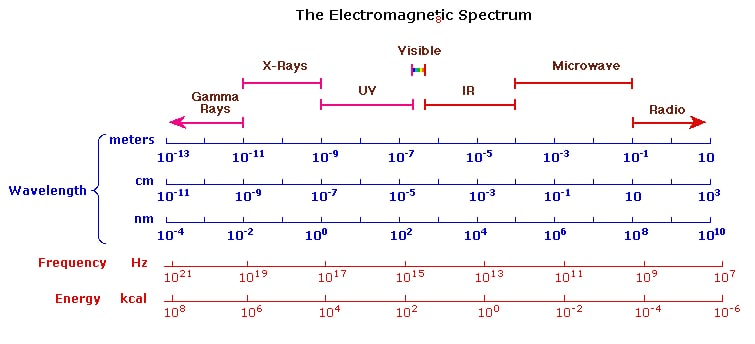
\includegraphics[width=0.7\textwidth]{3.Conceptos_Previos/emspec.jpg}
    \caption{Representación del espectro electromagnético con las longitudes de onda, frecuencias y energías asociadas. \\ Fuente: \cite{WikiLecturesSpectrum}.}
    \label{fig:emspec}
\end{figure}

El espectro electromagnético abarca todas las formas de radiación, desde los rayos gamma (longitudes de onda ultracortas) hasta las ondas de radio (longitudes de onda largas). Cada elemento químico absorbe o emite radiación en frecuencias específicas, actuando como una "huella digital" única. Estas interacciones se miden mediante espectrómetros, que identifican los patrones de absorción para determinar la composición química de un objeto o atmósfera. La detección satelital aprovecha estas propiedades para analizar gases en la Tierra, seleccionando bandas espectrales donde la señal del gas objetivo es clara y diferenciable de interferencias.

\subsubsection{Ventanas de observación y transmitancia atmosférica}
\begin{figure}[H]
    \centering
    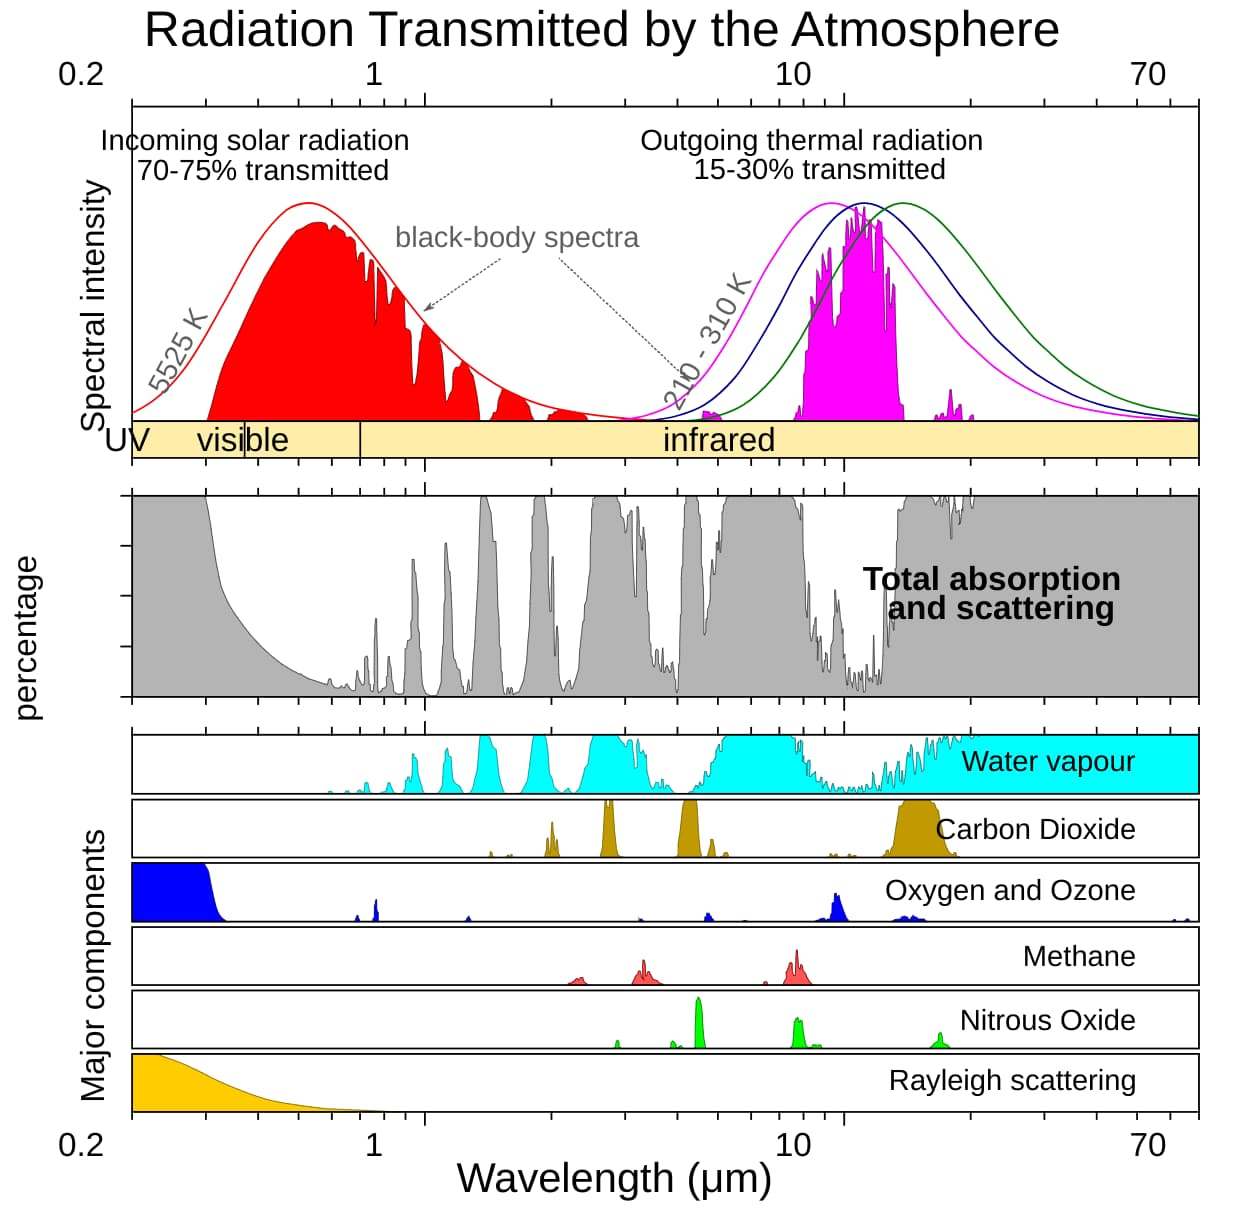
\includegraphics[width=0.7\textwidth]{3.Conceptos_Previos/Atmospheric_Transmission-en.jpg} 
    \caption{Radiación transmitida por la atmósfera y bandas de absorción. \\Fuente: \cite{atmospheric_transmission_spectrum}.}
    \label{fig:atm_transmission}
\end{figure}

La atmósfera terrestre no es transparente a todas las longitudes de onda. Gases como el CO$_2$, el vapor de agua y el ozono absorben fuertemente en regiones específicas, creando "bandas de absorción" que bloquean la radiación. Por ejemplo, el vapor de agua absorbe en el infrarrojo medio (6–8 $\mu$m) y el ozono en el ultravioleta (200–300 nm). Sin embargo, existen "ventanas atmosféricas" donde la radiación atraviesa con menor interferencia, como la región de 8–12 $\mu$m (infrarrojo térmico) y 14–16 $\mu$m (infrarrojo lejano). Estas ventanas son críticas para la teledetección, ya que permiten a los satélites capturar la radiación emitida o reflejada por la superficie terrestre \cite{wilber_surface_1999}.

\subsubsection{Bandas de absorción del CO\textsubscript{2}}

\begin{figure}[H]
    \centering
    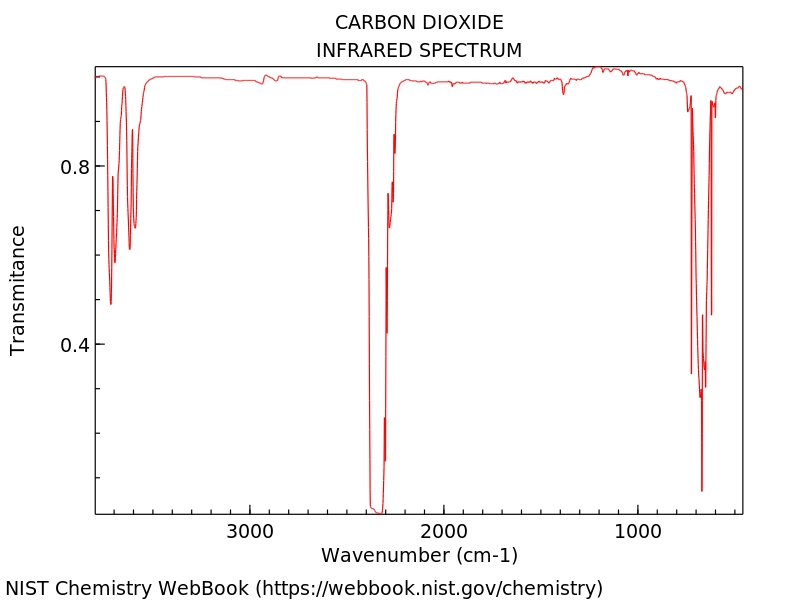
\includegraphics[width=1\textwidth]{3.Conceptos_Previos/cbook.cgi-2.png}
    \caption{Bandas de Transmitancia del CO$_2$ en función del número de onda.\\Fuente: \cite{nist2025co2_spectrum} }
    \label{fig:co2trans}
\end{figure}

El CO$_2$ presenta bandas de absorción características en diferentes regiones espectrales. Las bandas de 1,6 $\mu$m y 2,01 $\mu$m en el infrarrojo cercano son utilizadas por satélites como OCO-2 y GOSAT para medir la concentración columnar de CO$_2$ (XCO$_2$) mediante análisis de reflectancia solar. Estas bandas permiten la detección de CO$_2$ atmosférico aprovechando la absorción en la radiación solar reflejada por la superficie terrestre \cite{oco2_technical_specs_2024}.


La banda de 14--16 $\mu$m, aunque presenta fuerte absorción de CO$_2$, resulta inadecuada para mediciones de concentración desde plataformas espaciales. Esta banda mide principalmente temperatura atmosférica en lugar de concentraciones de CO$_2$, ya que la opacidad atmosférica impide la penetración hasta niveles superficiales donde ocurren las emisiones antropogénicas. Los algoritmos de recuperación requieren perfiles de temperatura extremadamente precisos, introduciendo incertidumbres que complican la separación entre efectos térmicos y variaciones de concentración. La fuerte absorción del CO$_2$ en 15 $\mu$m genera opacidad atmosférica elevada que limita la radiación detectada a niveles de la alta atmósfera, reduciendo significativamente la sensibilidad a las concentraciones cerca de la superficie terrestre \cite{pmc_co2_absorption_2018}.



\section{Detectores}

Los detectores de imágenes utilizados en satélites de observación son dispositivos electrónicos que convierten la radiación electromagnética en señales eléctricas. Este proceso se basa en el efecto fotoeléctrico, mediante el cual los fotones incidentes generan pares electrón-hueco en materiales semiconductores. Los detectores modernos se componen de matrices de píxeles, capaces de acumular carga eléctrica proporcional a la intensidad de la radiación recibida. Su estructura básica incluye una capa fotosensible de silicio u otro material semiconductor, junto con componentes electrónicos para la gestión, amplificación y lectura de estas cargas.

Para operar en el espacio, estos detectores deben superar condiciones particularmente exigentes: radiación cósmica, variaciones extremas de temperatura y ausencia de mantenimiento físico. Además, se requiere alta sensibilidad en las longitudes de onda de interés, bajo nivel de ruido para detectar señales débiles y un consumo energético reducido, dado que las plataformas satelitales disponen de recursos limitados. Parámetros como la resolución espacial, temporal y radiométrica son determinantes en la calidad de los datos adquiridos y su utilidad en distintas aplicaciones científicas y operativas \cite{kuroda_essential_2014}.

\subsection{Tipos de detectores}

\subsubsection{Sensores CCD (Charge-Coupled Device)}

\begin{figure}[H]
    \centering
    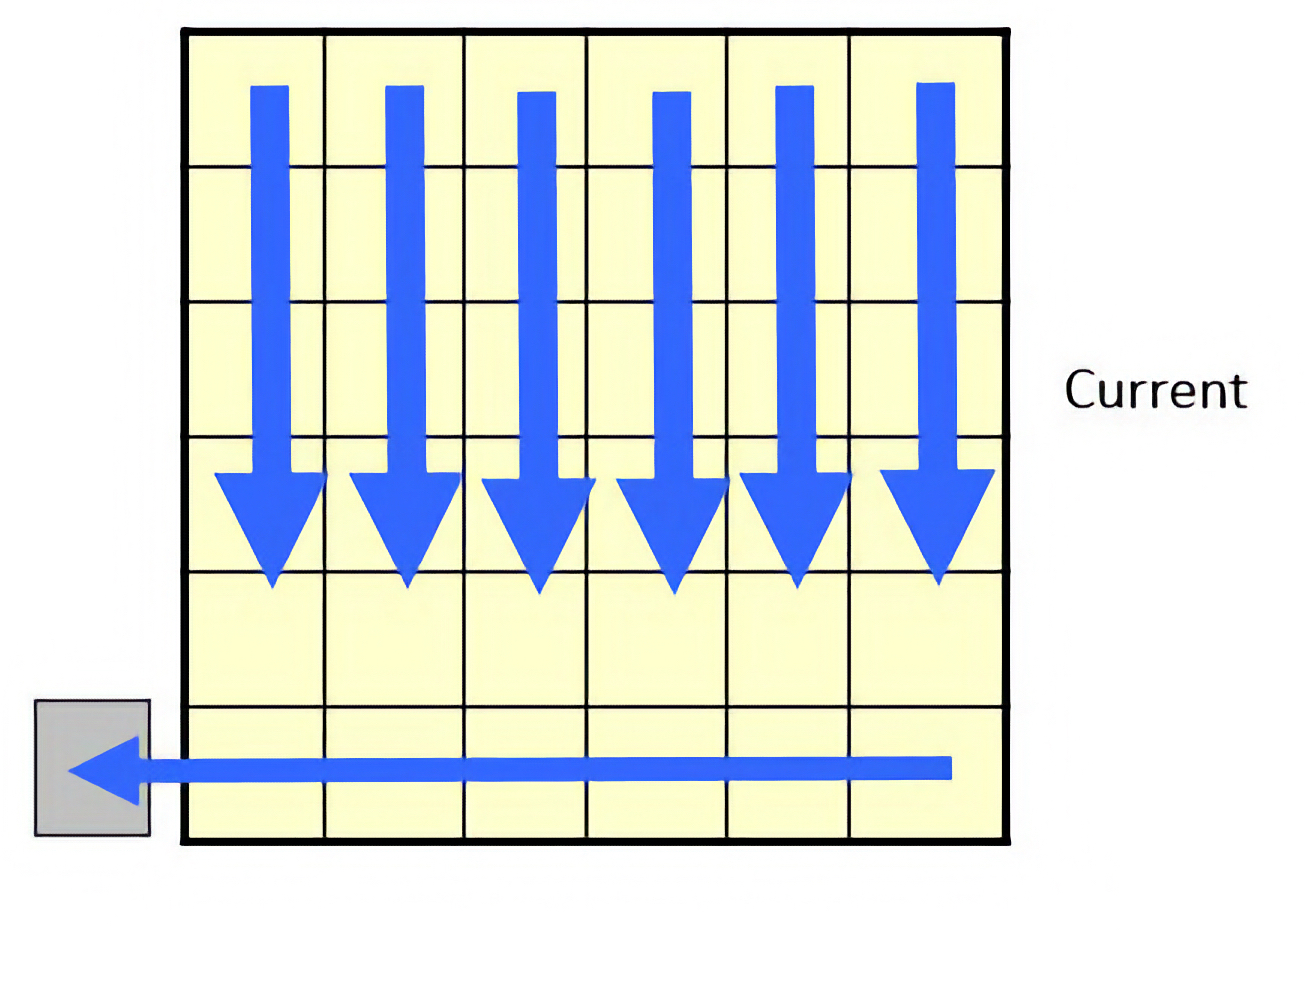
\includegraphics[width=0.7\textwidth]{3.Conceptos_Previos/CCD.jpg}
    \caption{Diagrama de funcionamiento de un sensor CCD.\\ Fuente: \cite{ccd_operation_diagram}.}
    \label{fig:CCD}
\end{figure}

Los sensores CCD (Dispositivo de Carga Acoplada) han sido durante años el estándar en misiones de observación espacial, gracias a su excelente calidad de imagen y desempeño en condiciones de baja iluminación. Funcionan acumulando carga en pozos de potencial dentro de un sustrato semiconductor, transfiriendo luego estas cargas secuencialmente a un nodo de salida para su lectura.

Destacan por su amplio rango dinámico, que puede duplicar al de los CMOS, y su bajo ruido de lectura, ideal para observaciones nocturnas o en bandas espectrales de baja radiancia. Presentan una notable uniformidad entre píxeles, reduciendo el ruido de patrón fijo y facilitando la calibración radiométrica. Además, al tener menos electrónica integrada en cada píxel, ofrecen un mayor factor de llenado, aprovechando mejor el área fotosensible.

Como aspectos menos favorables, presentan un consumo energético elevado, lo que puede ser un inconveniente en plataformas con recursos limitados. La dependencia de electrónica externa incrementa volumen y masa del sistema. También pueden sufrir el efecto \textit{blooming}, donde un píxel saturado afecta a los adyacentes, y su velocidad de lectura, relativamente baja, restringe su capacidad para captar escenas dinámicas. Asimismo, su sensibilidad a la radiación espacial puede degradar su rendimiento en misiones prolongadas \cite{kuroda_essential_2014}.

\subsubsection{Sensores CMOS (Complementary Metal-Oxide Semiconductor)}

\begin{figure}[H]
    \centering
    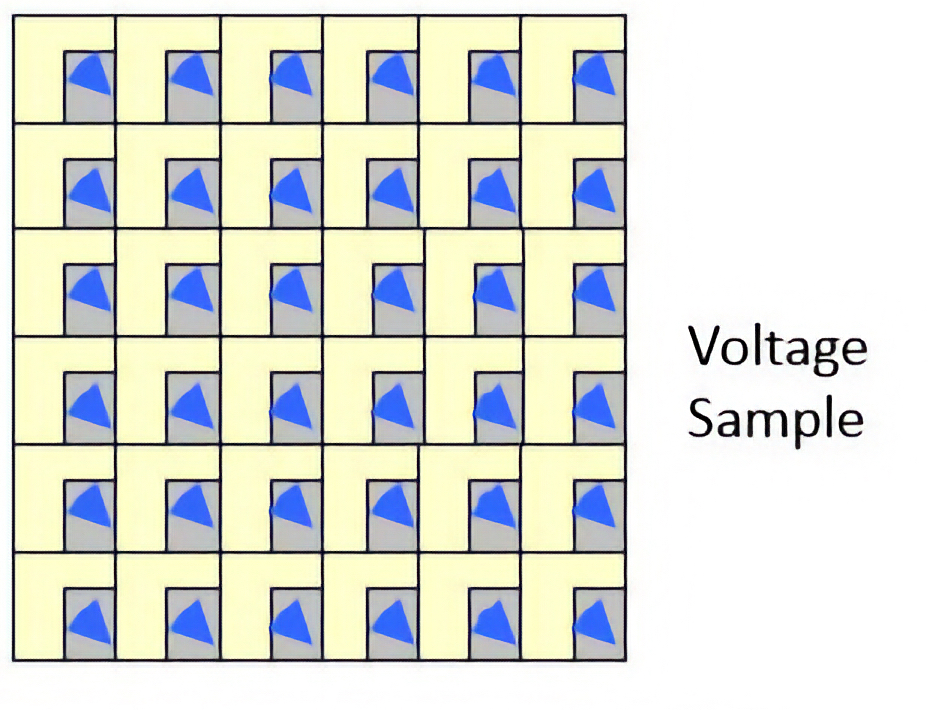
\includegraphics[width=0.7\textwidth]{3.Conceptos_Previos/CMOS.jpg}
    \caption{Diagrama de funcionamiento de un sensor CMOS.\\Fuente: \cite{ccd_operation_diagram}.}
    \label{fig:CMOS}
\end{figure}
Los sensores CMOS han ganado protagonismo en aplicaciones espaciales en los últimos años, debido a sus ventajas operativas en entornos con restricciones de recursos. A diferencia de los CCD, los CMOS integran circuitos de amplificación y procesamiento en cada píxel, permitiendo lecturas directas y selectivas.

Entre sus ventajas sobresalen su bajo consumo energético, típicamente entre una décima y una centésima parte del de un CCD comparable. Permiten lecturas parciales a alta velocidad, facilitando modos operativos flexibles, y su integración de funciones adicionales en el chip simplifica los sistemas, reduciendo su masa. También presentan una mayor tolerancia a la radiación, lo que los hace atractivos para misiones prolongadas.

Como desafíos, los primeros sensores CMOS mostraban mayores niveles de ruido de lectura y ruido de patrón fijo, aunque los desarrollos recientes han mitigado estas diferencias. El menor factor de llenado, debido a la electrónica en cada píxel, se compensa actualmente con microlentes que concentran la luz. Otro aspecto a considerar es el fenómeno \textit{rolling shutter}, que puede distorsionar imágenes con objetos en rápido movimiento, aunque las versiones con \textit{global shutter} resuelven este inconveniente. Finalmente, su sensibilidad en condiciones de baja iluminación, anteriormente inferior a la de los CCD, ha mejorado considerablemente con las tecnologías retroiluminadas \cite{kuroda_essential_2014}.

\subsubsection{Sensores HgCdTe}

\begin{figure}[H]
    \centering
    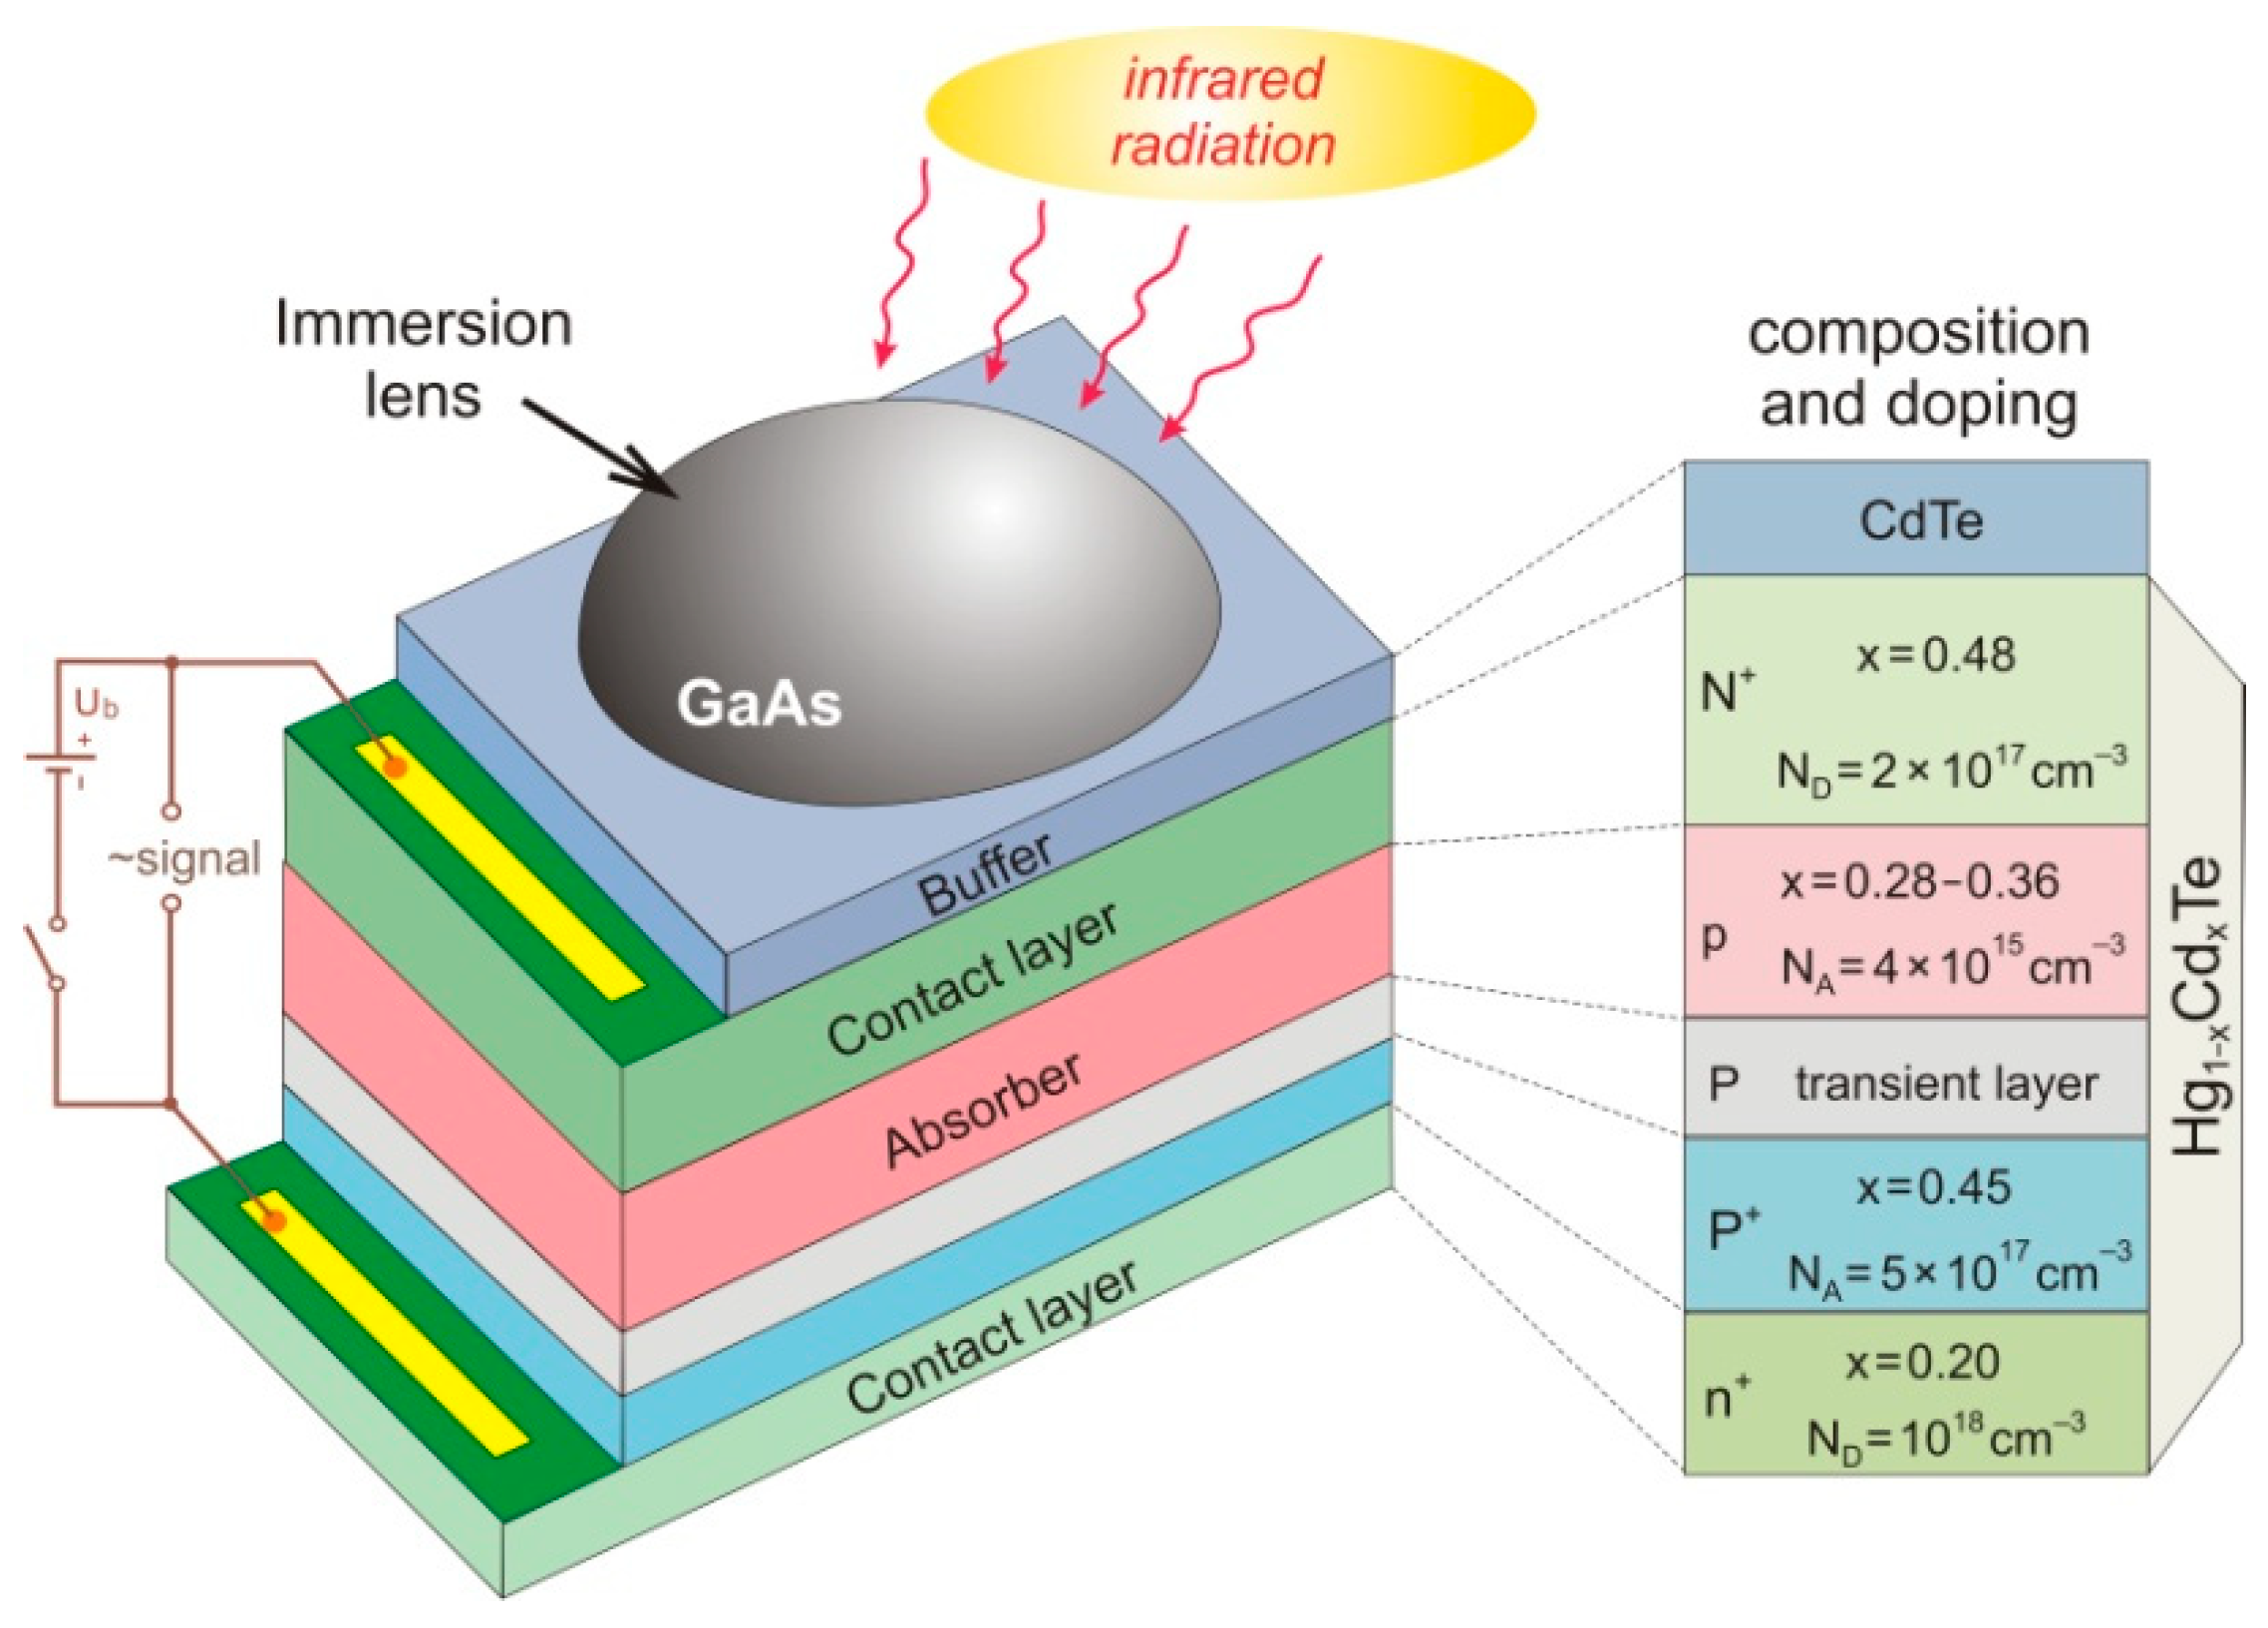
\includegraphics[width=0.5\linewidth]{3.Conceptos_Previos/coatings-11-00611-g002-2725805712.png}
    \caption{Disposición del detector MCT.\\Fuente: \cite{coatings2021_11_5_611_extended}.}
    \label{fig:enter-label}
\end{figure}

Los sensores de telururo de mercurio y cadmio (abreviado como MCT o HgCdTe) son reconocidos por su versatilidad espectral, con un rango ajustable entre 1 y 30 \textmu m mediante variaciones en la composición de la aleación. Esta adaptabilidad, unida a una eficiencia cuántica excepcional y tiempos de respuesta en nanosegundos, los posiciona como estándar en aplicaciones críticas como imágenes térmicas militares, astronomía infrarroja y detección de gases. Sus ventajas incluyen la capacidad de operar en modos fotoconductivo y fotovoltaico, alta detectividad incluso a temperaturas cercanas a ambiente y la posibilidad de crear estructuras de banda prohibida graduada para optimizar la absorción de fotones. Sin embargo, enfrentan desafíos como la toxicidad intrínseca del mercurio, que complica su fabricación y disposición final, y la sensibilidad a defectos cristalográficos durante el crecimiento epitaxial, lo que eleva los costos y reduce el rendimiento en dispositivos de gran área. Además, requieren sistemas de enfriamiento avanzados (criogénicos o mediante efecto Peltier) para minimizar el ruido térmico en aplicaciones de alta precisión, incrementando la complejidad del sistema global. A pesar de esto, siguen siendo insustituibles en aplicaciones que exigen cobertura espectral amplia y gran resolución térmica \cite{capper_mercury_2010}.

\subsubsection{Sensores InGaAs}


\begin{figure}[H]
    \centering
    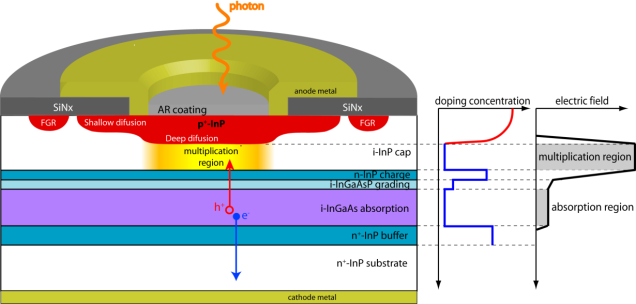
\includegraphics[width=0.5\linewidth]{3.Conceptos_Previos/ingaas_cross-1213932152.png}
    \caption{Disposición de capas típica del detector InGaAs. \\Fuente: \cite{everyphotoncounts2025ingaas_spad}.}
    \label{fig:enter-label}
\end{figure}

Los sensores de arseniuro de galio e indio (InGaAs) destacan por su capacidad para detectar radiación en el infrarrojo cercano (NIR), con un rango espectral típico entre 0,9 y 1,7 \textmu m, extendible hasta 2,55 \textmu m en versiones especializadas. Su estructura híbrida combina fotodiodos de InGaAs con circuitos CMOS, aprovechando una alta eficiencia cuántica y baja corriente oscura, lo que los hace ideales para aplicaciones que requieren precisión en condiciones de baja luminosidad. Entre sus ventajas destacan la sensibilidad extendida en el NIR, la capacidad de operar con requisitos de enfriamiento moderados y la ausencia de materiales tóxicos como el mercurio o el cadmio, cumpliendo con regulaciones ambientales. No obstante, presentan limitaciones como un ruido de corriente oscura significativo en entornos de alta temperatura, costos elevados debido a los procesos de fabricación complejos y fragilidad mecánica que exige manipulación cuidadosa. Además, su rendimiento en longitudes de onda superiores a 2 \textmu m tradicionalmente ha sido inferior al de otras tecnologías, aunque avances recientes están mitigando esta brecha \cite{henini_handbook_2002}.


\subsection{\textit{Time Delay and Integration} (TDI)}\label{sec:tdi}

\begin{figure}[H]
    \centering
    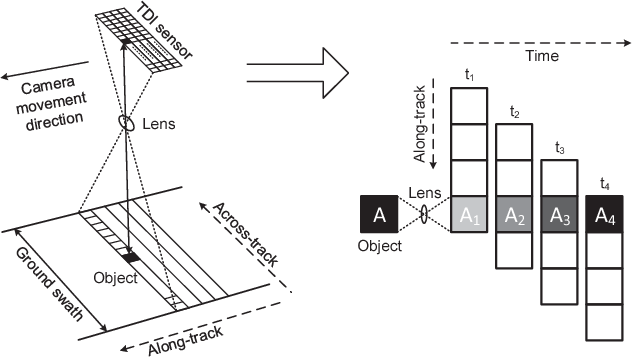
\includegraphics[width=0.7\textwidth]{3.Conceptos_Previos/TDI.png}
    \caption{Esquema de funcionamiento del \textit{Time Delay Integration}.\\Fuente: \cite{tdi_sensor2017}.}
    \label{fig:TDI}
\end{figure}

El TDI permite aumentar el tiempo efectivo de exposición sin desenfoque por movimiento, mejorando la relación señal-ruido en condiciones de baja iluminación o cuando se requieren tiempos de integración cortos debido a la velocidad de desplazamiento\cite{design_workshop_optical_2023}.

Consiste en una serie de líneas de píxeles que capturan sucesivamente la misma escena, desplazando la carga generada de una línea a otra en sincronía con el movimiento de la imagen sobre el detector. Esto permite acumular la carga correspondiente a un mismo punto a lo largo de varias etapas, aumentando efectivamente el tiempo de exposición.

Esta técnica exige una sincronización precisa entre la velocidad de transferencia de carga y la velocidad de desplazamiento de la imagen proyectada. Cualquier desajuste afectaría la resolución espacial, provocando desenfoque. Al multiplicar el tiempo de exposición por el número de etapas, permite mejorar notablemente la sensibilidad sin sacrificar resolución espacial.


\subsection{Estrategias de Escaneo en Sistemas de Observación Satelital}

Para adquirir imágenes de la superficie terrestre desde una órbita, resulta indispensable definir una estrategia de escaneo que permita cubrir progresivamente la zona de interés. Estas estrategias determinan cómo se captura la información espacial y temporalmente, considerando tanto la configuración del detector como el movimiento relativo entre el satélite y la superficie terrestre. A continuación, se describen las principales técnicas empleadas en sistemas de observación orbital, junto con sus ventajas, limitaciones y ámbitos de aplicación característicos\cite{design_workshop_optical_2023}.


\subsubsection{Tecnología Pushbroom (Barrido Lineal)}

\begin{figure}[H]
    \centering
    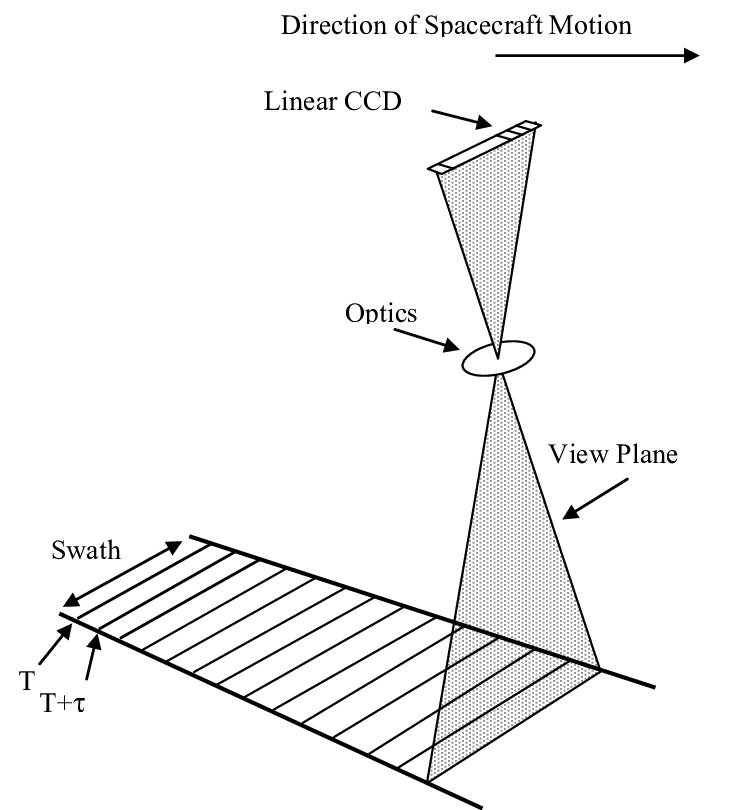
\includegraphics[width=0.7\textwidth]{3.Conceptos_Previos/Pushbroom.png}
    \caption{Funcionamiento del escaneo \textit{Pushbroom}.\\Fuente: \cite{pushbroom_sensor_diagram}.}
    \label{fig:Pushbroom}
\end{figure}


La tecnología Pushbroom es una de las más utilizadas actualmente en observación terrestre desde satélites. Utiliza una línea de detectores dispuestos perpendicularmente a la dirección de vuelo. Esta línea captura simultáneamente una franja del terreno, mientras que el movimiento orbital permite generar la imagen completa.

Sus ventajas incluyen una mayor relación señal-ruido gracias al tiempo de observación más prolongado sobre cada punto y la ausencia de componentes mecánicos móviles, lo que aumenta su fiabilidad. Como desafío, presenta variaciones en la sensibilidad entre detectores individuales que pueden provocar franjas si no se calibra adecuadamente. Además, suele ofrecer una resolución espacial ligeramente inferior a los escáneres Whiskbroom para un mismo ancho de barrido.

\subsubsection{Tecnología Whiskbroom (Barrido Transversal)}

\begin{figure}[H]
    \centering
    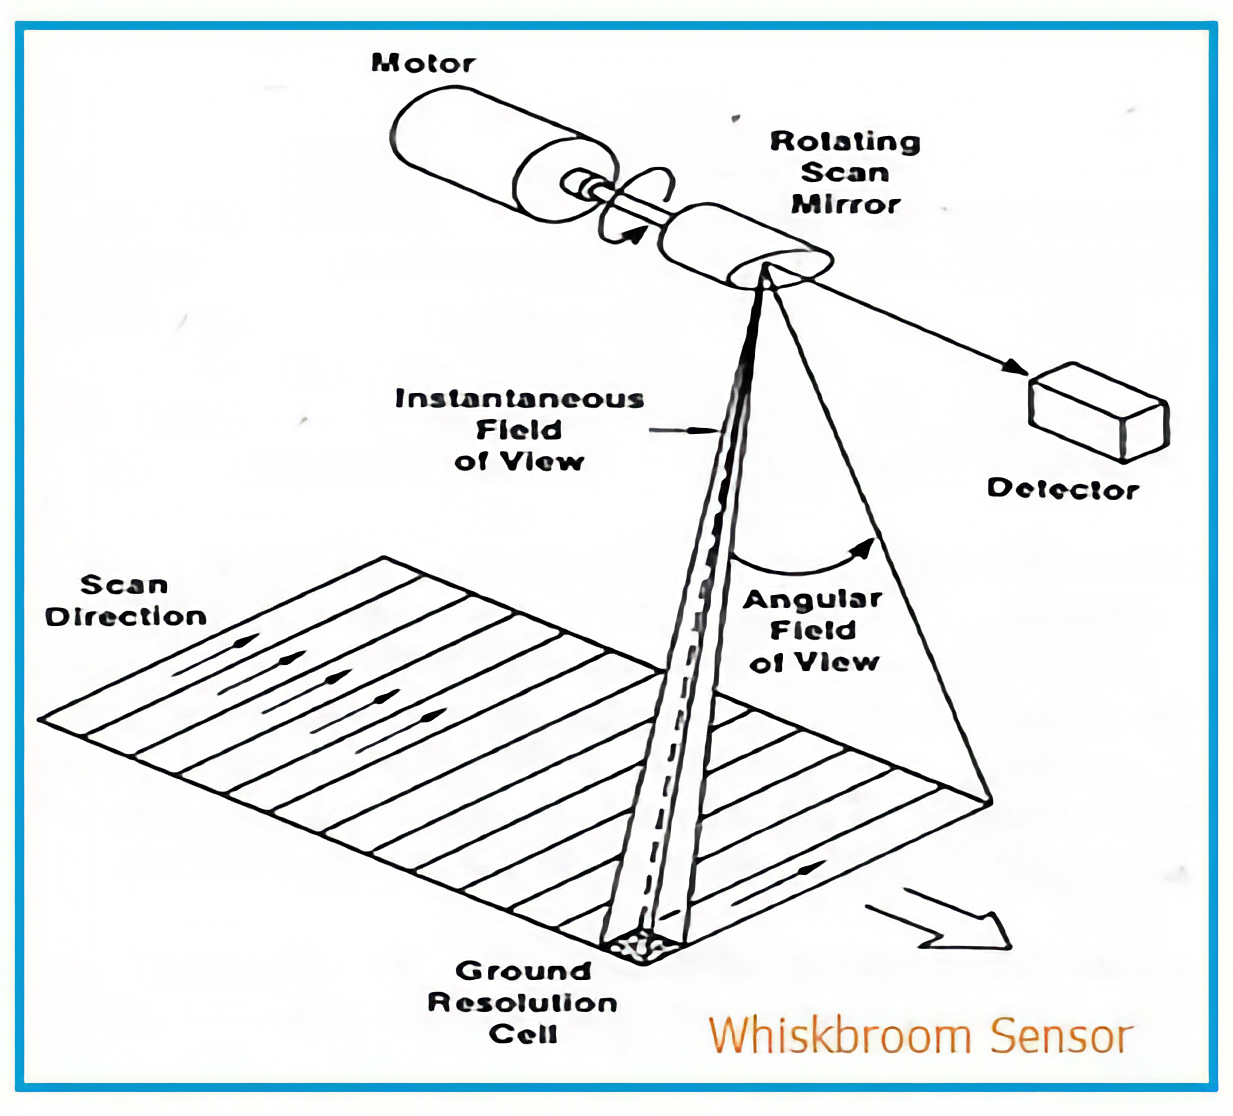
\includegraphics[width=0.7\textwidth]{3.Conceptos_Previos/whiskbroom.jpg}
    \caption{Funcionamiento del escaneo \textit{Whiskbroom}.\\Fuente: \cite{whiskbroom_diagram}.}
    \label{fig:whiskbroom}
\end{figure}

Los escáneres Whiskbroom funcionan mediante un espejo oscilante que barre perpendicularmente a la trayectoria del satélite, dirigiendo la luz hacia uno o pocos detectores.

Su principal ventaja es la alta resolución espacial alcanzable, ya que permite concentrar la observación en pequeñas áreas mediante un número reducido de detectores, facilitando la uniformidad radiométrica. Como contrapartida, incorporan componentes mecánicos móviles que aumentan el peso y la complejidad, y su menor tiempo de observación por píxel limita su sensibilidad en condiciones de baja iluminación. Además, su naturaleza secuencial restringe la velocidad máxima de adquisición.

\subsubsection{Enfoque Step-Stare (Configuración de Imagen Estática)}

\begin{figure}[H]
    \centering
    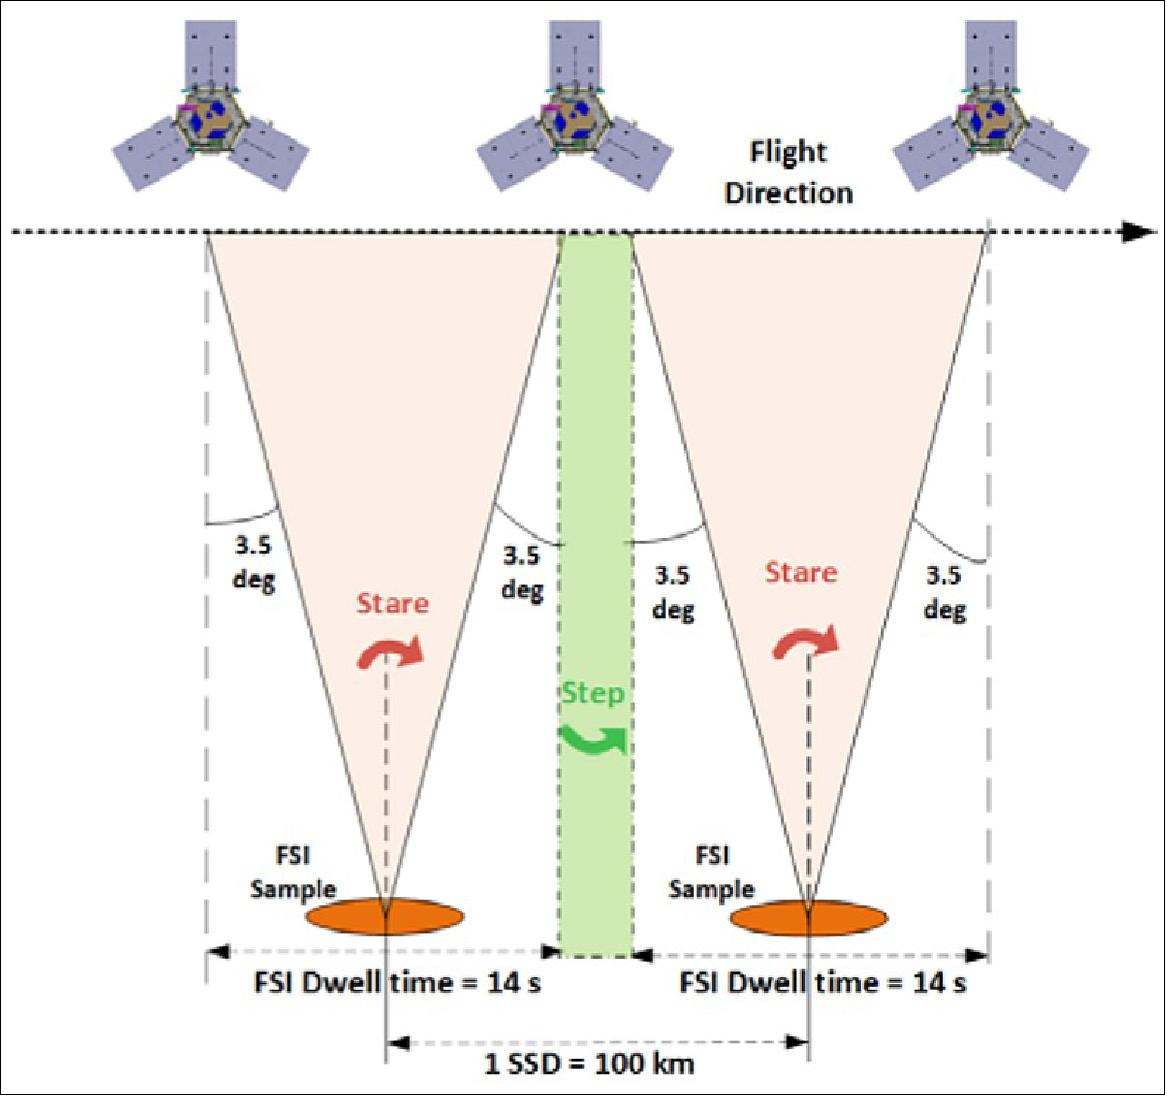
\includegraphics[width=0.7\textwidth]{3.Conceptos_Previos/Step Stare.jpeg}
    \caption{Funcionamiento del escaneo \textit{Step-Stare}.\\Fuente: \cite{step_stare_system}.}
    \label{fig:Stepstare}
\end{figure}

El enfoque Step-Stare captura imágenes bidimensionales completas de forma discreta, similar a una cámara fotográfica. Entre exposiciones, el sistema óptico se reorienta hacia la siguiente área de interés.

Esta configuración maximiza la eficiencia en la recolección de fotones al dedicar todo el tiempo de exposición a cada imagen, logrando excelente relación señal-ruido. Permite también apuntamiento flexible, ideal para monitoreo de emergencias o eventos dinámicos. Como aspectos a considerar, requiere compensar el movimiento de la plataforma para evitar desenfoque y presenta menor eficiencia en la cobertura continua de grandes áreas, debido al tiempo adicional necesario para reposicionar el sistema entre capturas.

\subsection{Disposición de detectores}

En el diseño del plano focal para la carga útil óptica, la disposición de los detectores es un aspecto clave que afecta tanto la calidad de imagen como la viabilidad técnica y económica del satélite. Existen varias estrategias para el \textit{layout} de detectores, entre las que destacan \cite{kaplan_optical_2011}:

\begin{itemize}
    \item \textbf{Divisores de campo (Divoli o \textit{Field Splitters})}: Esta solución emplea elementos ópticos para dividir el campo de visión en regiones independientes, cada una dirigida a un detector específico. Permite optimizar la captación de diferentes bandas espectrales o maximizar el área cubierta por cada detector, facilitando la especialización de cada canal detector para una banda concreta o para mejorar la redundancia y la relación señal/ruido (SNR) en segmentos críticos del espectro.

    \item \textbf{Divisores de haz (\textit{Beam Splitters})}: Utilizados para separar la luz en distintas longitudes de onda y redirigirlas a detectores diferentes. Esta técnica es útil cuando se requieren bandas espectrales muy diferenciadas, aunque introduce pérdidas ópticas y puede complicar el alineamiento y la calibración radiométrica.

    \item \textbf{Solapamiento parcial de detectores}: En algunos diseños, se solapan parcialmente las áreas sensibles de los detectores para mejorar la corregistración entre bandas o aumentar la redundancia. Sin embargo, esto incrementa la complejidad del procesamiento y puede penalizar la eficiencia espacial y el peso del sistema.
\end{itemize}

A la hora de dimensionar la misión, se establece un límite máximo de \textbf{tres detectores}, con el fin de simplificar la disposición de los mismos \cite{design_workshop_optical_2023}.

\section{Óptica. Telescopios}

La óptica de un satélite de observación es el conjunto de elementos (lentes, espejos, filtros, etc.) que recogen la radiación electromagnética proveniente de la Tierra y la enfocan sobre el detector. El telescopio es el corazón de este sistema óptico: su función es formar una imagen nítida y de alta calidad sobre el plano focal, maximizando la resolución espacial y la eficiencia de captación de luz, minimizando aberraciones y pérdidas de contraste.
La elección del tipo de telescopio depende de los requisitos de la misión (resolución, campo de visión, peso, facilidad de alineamiento y fabricación, etc.). Los diseños más usados en teledetección espacial son los telescopios refractivos y los reflectores de dos o tres espejos (Cassegrain, Korsch, TMA) \cite{design_workshop_optical_2023}.

\subsection{Parámetros ópticos relevantes}

\begin{figure}[H]
    \centering
    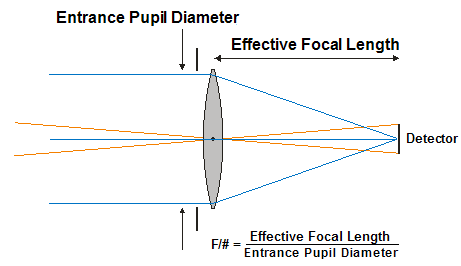
\includegraphics[width=0.7\textwidth]{3.Conceptos_Previos/eoirOptical1.png}
    \caption{Diagrama de parámetros ópticos. \\Fuente: \cite{entrance_pupil_diagram}.}
    \label{fig:Lente}
\end{figure}

\subsubsection*{Diámetro de pupila ($D$)}

El diámetro de pupila es el tamaño de la apertura circular por la que entra la luz al sistema óptico, también conocido como apertura del telescopio. Este parámetro es crucial porque determina la cantidad de luz que puede captar el sistema (afectando a la SNR) y el límite de difracción, es decir, la máxima resolución teórica que puede alcanzar el instrumento. Un mayor diámetro de pupila permite captar más luz y obtener una mejor resolución espacial, pero también incrementa el peso y el tamaño del instrumento, lo que es crítico en satélites donde se busca minimizar la masa para reducir costes de lanzamiento.

\subsubsection*{Distancia focal ($f$)}

La distancia focal es la separación entre el centro óptico del sistema (o el espejo principal, en sistemas reflectores) y el plano focal donde se forma la imagen. Este parámetro define el aumento del sistema: a mayor distancia focal, mayor es la imagen proyectada sobre el detector para un mismo objeto observado en la Tierra. En instrumentos de observación, la distancia focal se elige para cumplir con el GSD requerido, ya que está relacionada con el tamaño del píxel del detector y la resolución en superficie.

\subsubsection*{Relación focal ($F\#$)}

La relación focal se define como el cociente entre la distancia focal y el diámetro de pupila ($F\#=\frac{f}{D}$). Para los sistemas obscurados, se define la relación focal equivalente $T\#$, que viene dada por la relación:
\begin{align}
\label{relfoc}
    T\# = \frac{f}{\sqrt{D^2(1-R_{obs}^2)}} 
\end{align}

Siendo $R_{obs}$ la misma relación de obscuración en la ecuación \ref{mtfrobs}
Es un parámetro clave ya que in número $F\#$ bajo (óptica “rápida”) implica una apertura grande respecto a la distancia focal, lo que permite captar más luz y mejora la SNR, pero puede aumentar las aberraciones ópticas y reducir la profundidad de campo. Un número $F\#$ alto (óptica “lenta”) reduce la cantidad de luz captada, pero suele simplificar el diseño y controlar mejor las aberraciones. La relación focal afecta directamente a la MTF, la SNR y la saturación del detector.


\subsection{Tipos de telescopio}


\subsubsection{Refractivo}

\begin{figure}[H]
    \centering
    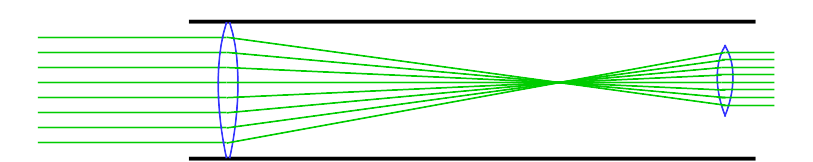
\includegraphics[width=0.7\textwidth]{3.Conceptos_Previos/refractor-vs-reflector-4239218127.png}
    \caption{Telescopio Refractivo. \\ Fuente: \cite{refractor_reflector_comparison}.}
    \label{fig:Refractive}
\end{figure}

El telescopio refractivo utiliza lentes para enfocar la luz sobre el detector. Su principal ventaja es la ausencia de obscuración, ya que toda la apertura está disponible para captar luz. Esto se traduce en una MTF de difracción más alta, especialmente a frecuencias espaciales elevadas, y en una penalización por alineamiento relativamente baja ($MTF_{alineamiento} \approx 0,90$), pues el sistema es sencillo de montar y ajustar. Sin embargo, los telescopios refractivos presentan aberraciones cromáticas, lo que limita su uso en aplicaciones multiespectrales o en longitudes de onda fuera del visible. Además, para grandes aperturas (entre 80 y 100 mm), las lentes se vuelven pesadas y difíciles de fabricar, lo que desincentiva su uso en satélites de observación de alta resolución, o de orbitas mayores a LEO (\textit{Low Earth Orbit}).


\subsubsection{Cassegrain}

\begin{figure}[H]
    \centering
    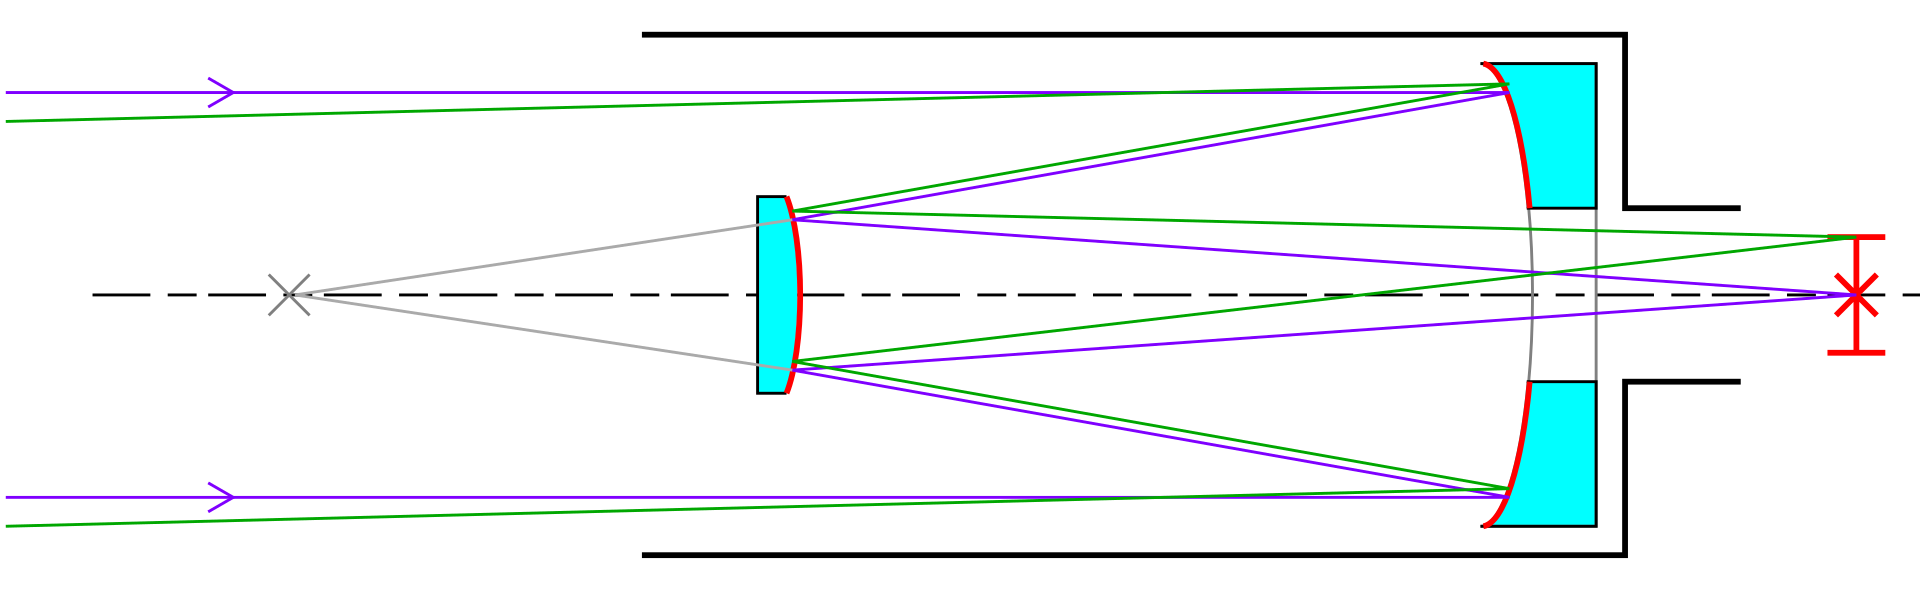
\includegraphics[width=0.7\textwidth]{3.Conceptos_Previos/Cassegrain_Telescope.svg.png}
    \caption{Telescopio Cassegrain. \\Fuente: \cite{cassegrain_telescope_diagram}.}
    \label{fig:Cassegrain}
\end{figure}

El diseño Cassegrain es un reflector de dos espejos, con un primario parabólico y un secundario hiperbólico. La luz se refleja primero en el espejo primario, luego en el secundario y finalmente pasa a través de un orificio en el primario hacia el detector. Este sistema introduce una obscuración central debida al secundario, lo que reduce la MTF de difracción a frecuencias altas, pero permite una configuración compacta y una buena corrección de aberraciones cromáticas. El alineamiento es moderadamente sencillo, con una penalización típica de $MTF_{alineamiento} \approx 0,85$. El campo de visión es limitado, típicamente en torno a 3°.

\subsubsection{Korsch}

\begin{figure}[H]
    \centering
    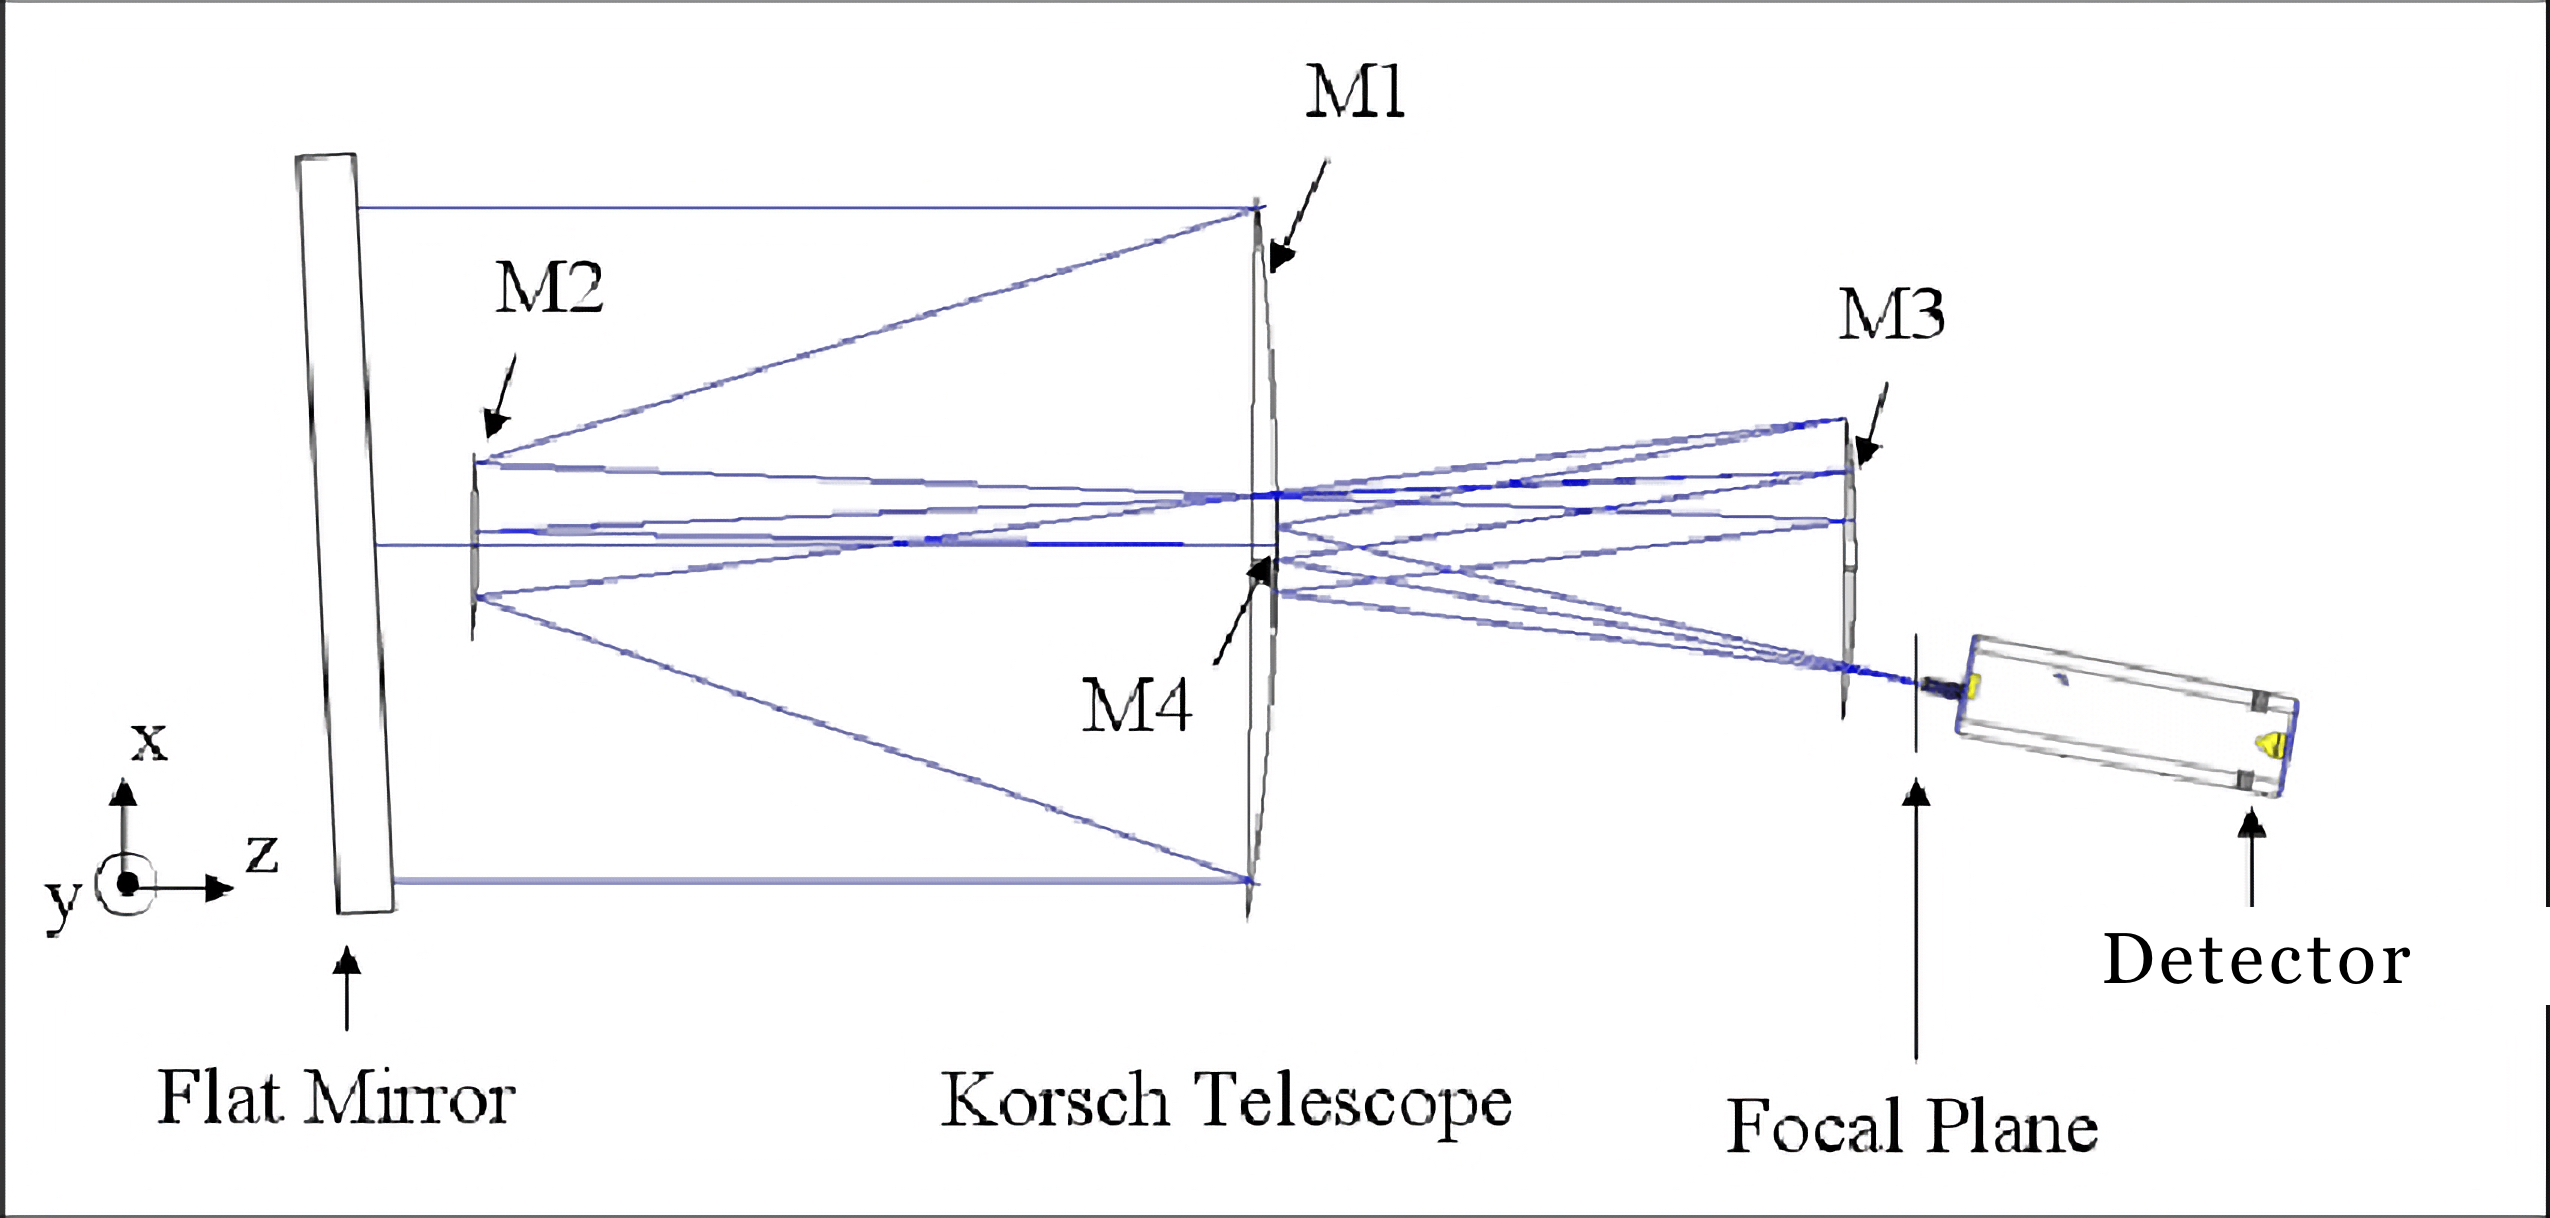
\includegraphics[width=0.7\textwidth]{3.Conceptos_Previos/Korsch.jpg}
    \caption{Telescopio Korsch. \\Fuente: \cite{korsch_telescope_system}.}
    \label{fig:Korsch}
\end{figure}

El telescopio Korsch es un reflector de tres espejos, también con obscuración central. Su diseño está optimizado para controlar la luz parásita (straylight). Permite focales largas y una buena calidad de imagen en todo el campo, aunque el alineamiento es más complejo y la penalización en la MTF por este motivo es mayor ($MTF_{alineamiento} \approx 0,80$). La presencia de la obscuración central sigue penalizando la MTF de difracción, aunque el control de aberraciones es excelente. Posee un FoV similar al Cassegrain, de $3º$.

\subsubsection{\textit{Three-mirror anastigmat} (TMA)}

\begin{figure}[H]
    \centering
    
\includegraphics[width=0.7\textwidth]{3.Conceptos_Previos/TMA.png}
    \caption{Telescopio TMA. \\Fuente: \cite{tma_telescope_diagram}.}
    \label{fig:Tma}
\end{figure}

El telescopio de tres espejos anastigmático es un reflector de tres espejos sin obscuración central, ya que el haz óptico se desvía fuera del eje óptico principal (diseño off-axis). Esto permite un campo de visión mas amplio, del orden de $8º$, y una calidad de imagen homogénea en todo el campo, sin penalización por la presencia de elementos que bloqueen la apertura. Sin embargo, el alineamiento de un TMA es extremadamente exigente, con una penalización en la MTF de alineamiento significativa ($MTF_{alineamiento} \approx 0,70$). Además, la fabricación y verificación de estos sistemas es más compleja y costosa.

\subsubsection*{Tabla comparativa de Telescopios}

\begin{table}[H]
\caption{Comparativa de tipos de sistemas ópticos.}
\centering
\begin{tabular}{l c c c c}
\hline
\textbf{Tipo} & \textbf{Obscuración($R_{obs}$)} & \textbf{$FoV_{lim}$} & \textbf{MTF\textsubscript{Alineamiento}} & \textbf{Transmisión óptica $(\tau)$} \\
\hline
Refractivo\tablefootnote{ Limitado a 80 mm de diámetro máximo válido para el presente trabajo}    & No  & 10º & 0,90 & 0,8 \\
Cassegrain    & Sí (0,2)  & 3º  & 0,85 & 0,7 \\
Korsch        & Sí (0,2)  & 3º  & 0,80 & 0,65 \\
TMA           & No  & 8º  & 0.70 & 0,6 \\
\hline
\end{tabular}

\label{tab:tabla_telescopios}
\end{table}



\subsection{Filtros}

\begin{figure}[H]
    \centering
    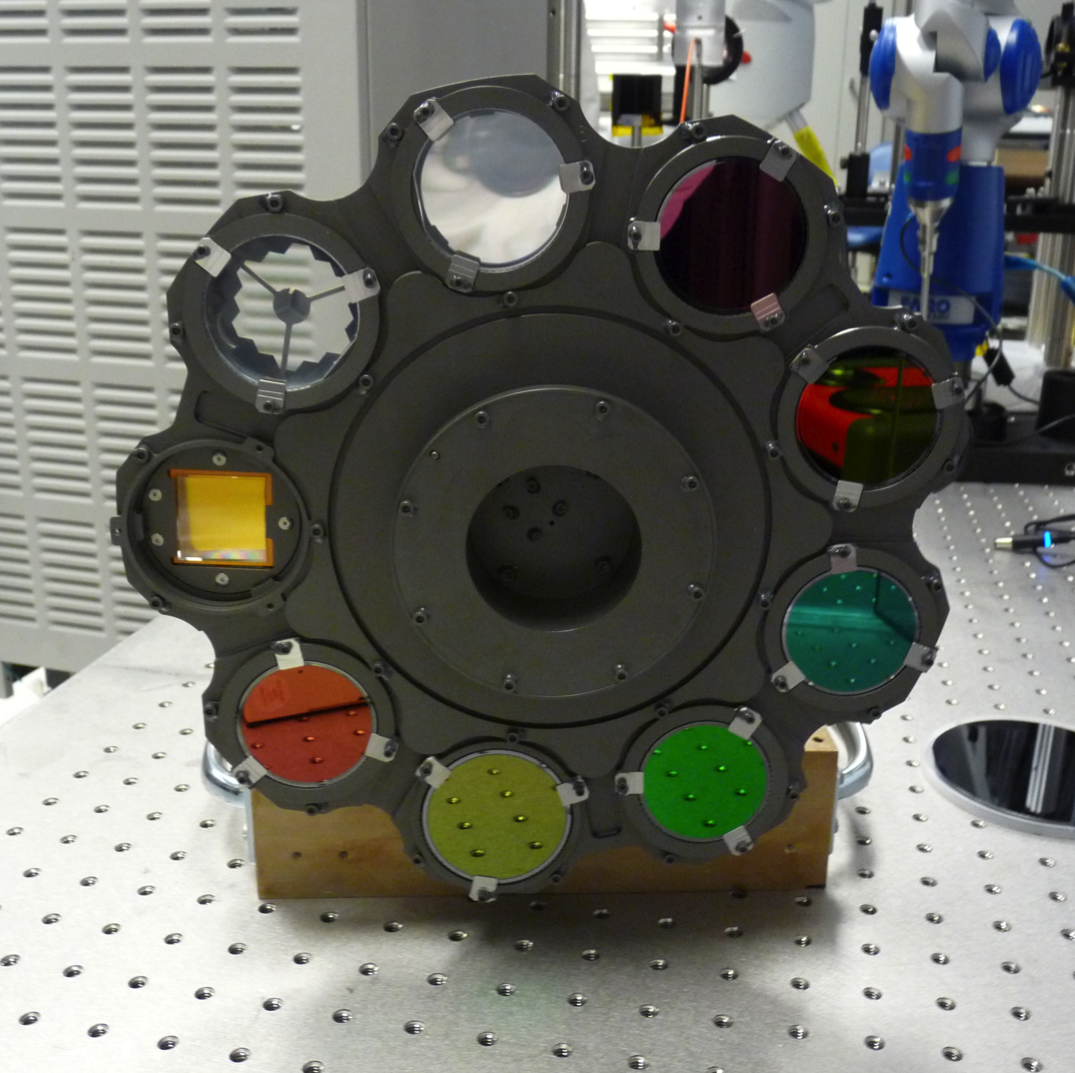
\includegraphics[width=0.7\textwidth]{3.Conceptos_Previos/NIRISS_FilterWheel.png}
    \caption{Rueda de Filtros del \textit{James Webb Space Telescope}. \\Fuente: \cite{STScI_MIRI_Filters}.}
    \label{fig:Filter}
\end{figure}

La selección de filtros ópticos en el detector es fundamental para definir las bandas espectrales de interés, optimizar la relación señal-ruido (SNR), garantizando la calidad radiométrica y espacial de la imagen.

Los filtros ópticos seleccionan las longitudes de onda que llegan al detector, permitiendo medir únicamente las bandas espectrales relevantes para el objetivo de la misión. 


\begin{figure}[H]
    \centering 
    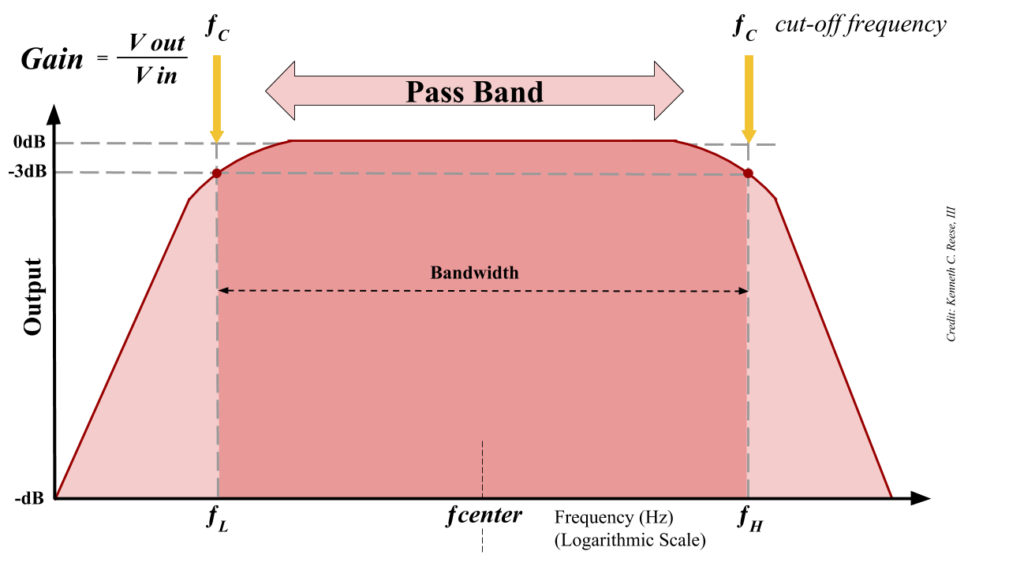
\includegraphics[width=0.7\textwidth]{3.Conceptos_Previos/bandpass-filter-fig-1-1024x577-2751970399.png}
    \caption{Filtrado de las frecuencias.\\ Fuente:\cite{Reeve2024BandPass}.}
    \label{fig:bandpass}
\end{figure}

La anchura de banda debe ser lo suficientemente estrecha para aislar las líneas de absorción de interés, pero lo suficientemente ancha para mantener una SNR adecuada. Los filtros deben tener alta transmitancia en la banda de interés para maximizar la señal y baja transmitancia fuera de banda para evitar contaminación espectral. Así mismo deben ser capaces de bloquear al máximo el resto de las bandas fuera de nuestro interés para reducir el ruido.

\subsubsection*{Tipos de Filtros y Configuración}


\begin{itemize}
    \item \textbf{Rueda de filtros}: Un solo detector y una rueda que posiciona secuencialmente diferentes filtros delante del detector. Es una solución asequible pero introduce partes móviles y puede limitar la velocidad de adquisición.
    
    \item \textbf{Módulos de filtro independientes}: Cada detector tiene su propio filtro fijo. Permite mayor robustez y elimina partes móviles, pero puede aumentar el tamaño del plano focal y dificultar la corregistración espacial.
    
    \item \textbf{Filtros tipo \textit{microstrip}}: Filtros miniaturizados directamente sobre el detector o muy próximos a él. Permiten una disposición compacta y robusta, adecuada para configuraciones multiespectrales con alta corregistración.
\end{itemize}





\section{Parámetros Orbitales}


\begin{figure}[H]
    \centering
    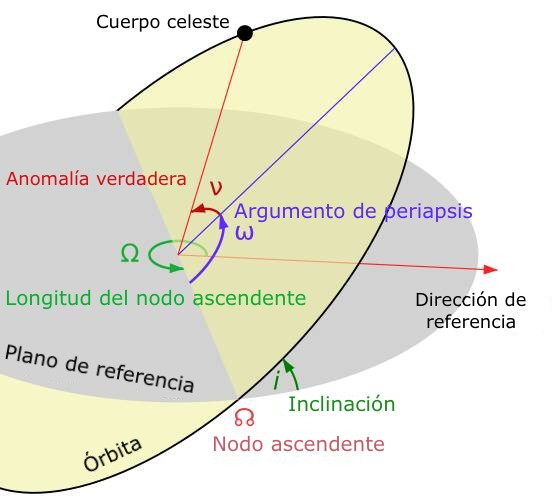
\includegraphics[width=0.5\linewidth]{3.Conceptos_Previos/Elementos_orbitales.jpg}
    \caption{Representación gráfica de los elementos orbitales. \\ Fuente: \cite{WikiElementosOrbitales}.
}
\end{figure}

A continuación se definen los principales parámetros que definen la órbita del cuerpo de interés, así como las perturbaciones asociadas de mayor peso en la mecánica orbital para el presente problema \cite{curtis2020orbital}.

\subsubsection*{Semieje mayor ($a$)}

El semieje mayor determina el tamaño básico de la órbita elíptica, representando la distancia desde el centro de la elipse hasta su extremo más alejado sobre el eje principal.

\subsubsection*{Excentricidad ($e$)}

La excentricidad define la forma de la órbita, como la desviación del cuerpo central respecto al centro geométrico de la elipse. Matemáticamente:

\begin{align}
e = \sqrt{1 - \frac{b^2}{a^2}}
\end{align}

donde \( b \) es el semieje menor. La excentricidad determina varios tipos de órbitas:

\begin{itemize}
    \item \( e = 0 \): Órbita perfectamente circular
    \item \( 0 < e < 1 \): Órbita elíptica (como la mostrada en las imágenes)
    \item \( e = 1 \): Trayectoria parabólica
    \item \( e > 1 \): Trayectoria hiperbólica
\end{itemize}

\noindent Estos parámetros no tendrán mucha relevancia en este trabajo como veremos más adelante, ya que por simplicidad escogeremos una orbita circular$(e\approx0)$. El semieje mayor se podrá resumir en la altura orbital,
definida como $h= a- R_T$, siendo $R_T$ el radio de la Tierra.

\subsection{Inclinación ($i$)}

La inclinación representa el ángulo entre el plano orbital y el plano de referencia (generalmente el ecuador terrestre). En la primera imagen se muestra como el ángulo formado entre estos dos planos. Para órbitas terrestres, se clasifica de la siguiente manera:

\begin{itemize}
  \item $i = 0^\circ$: Órbita ecuatorial
  \item $0^\circ < i < 90^\circ$: Órbita prógrada
  \item $i = 90^\circ$: Órbita polar
  \item $90^\circ < i < 180^\circ$: Órbita retrógrada
\end{itemize}

Este parámetro es crucial para determinar qué regiones de la Tierra sobrevolará el satélite.

\subsection{Longitud del Nodo Ascendente ($\Omega$)}

La longitud del nodo ascendente define la orientación del plano orbital en el espacio tridimensional. Como se visualiza en la primera imagen, es el ángulo medido desde la dirección de referencia hasta el nodo ascendente (punto donde la órbita cruza el plano de referencia en dirección norte). Este elemento es particularmente importante para órbitas heliosíncronas, donde precesa aproximadamente $1^\circ$ diario para mantener una relación constante con el Sol.

\subsection{Hora de paso local (LTAN)}

La hora de paso local en el nodo ascendente (\textit{Local Time of Ascending Node}, o LTAN) es el instante del día, medido en tiempo solar local, en que el satélite cruza el meridiano de su nodo ascendente. Es fundamental para misiones de observación de la Tierra, ya que determina las condiciones de iluminación solar en cada pasada.

Se calcula relacionando la longitud ascendente $\Omega$ con la posición del Sol en longitud eclíptica $\lambda_\odot(t)$, según:
\[
T_{\mathrm{LST}} 
= \frac{\Omega - \lambda_\odot(t)}{15^\circ}\quad[\mathrm{horas}],
\]
donde:
\begin{itemize}
  \item $\Omega$ es la longitud del nodo ascendente (°),
  \item $\lambda_\odot(t)$ es la longitud eclíptica del Sol en el instante $t$ (°),
  \item el factor $15^\circ/$h convierte grados en horas solares locales.
\end{itemize}

En la práctica se suele referir el LTAN a valores redondeados (por ejemplo, 10:30 h o 13:30 h) para garantizar escenas con sombras y contraste adecuados. En órbitas heliosíncronas, la precesión de $\Omega$ ($\approx$ 1º/día) se ajusta de modo que el LTAN permanezca prácticamente constante durante toda la misión.


\subsection{Argumento del Perigeo ($\omega$)}

El argumento del perigeo describe la orientación de la elipse dentro del plano orbital. En las figuras se muestra como el ángulo entre el nodo ascendente y el punto de máximo acercamiento al cuerpo central (perigeo). Este parámetro determina dónde se producirán las distancias mínima y máxima de la órbita. Para satélites científicos en órbitas excéntricas, este valor se elige cuidadosamente para sobrevolar determinadas regiones a la altura mínima. 

Debido a que en este estudio solo se aplicaran orbitas circulares ($e\approx0$), este parámetro carece de relevancia, pues no habrá un perigeo claramente definido.

\subsection{Anomalía Verdadera ($\nu$)}

La anomalía verdadera es el único elemento que varía con el tiempo para una órbita no perturbada. Representa la posición instantánea del cuerpo orbitante, medida como el ángulo desde el perigeo hasta la posición actual del satélite, en la dirección del movimiento.


\section{Perturbaciones de la órbita}

\subsection{Achatamiento Terrestre}

La Tierra no es perfectamente esférica; presenta un abultamiento en el ecuador debido a su rotación. Este achatamiento genera un campo gravitacional asimétrico que introduce una perturbación en las órbitas de los satélites. Este efecto provoca dos movimientos importantes en los elementos orbitales:

\begin{enumerate}
    \item \textbf{Regresión del nodo ascendente} (\( \Omega \)): El nodo ascendente, el punto donde la órbita cruza el ecuador de sur a norte, experimenta un movimiento de precesión regresiva.
    \item \textbf{Precesión del argumento del perigeo} (\( \omega \)): El argumento del perigeo también se ve afectado, lo cual es relevante para órbitas con cierta excentricidad.
\end{enumerate}

Estas perturbaciones dependen de la altitud, la inclinación y otros parámetros orbitales. En el próximo apartado (\ref{sec:SSO}) se detalla como acoplar dichas variables para definir órbitas heliosíncronas.



\subsection{Decaimiento Orbital}


\begin{figure}[H]
    \centering
    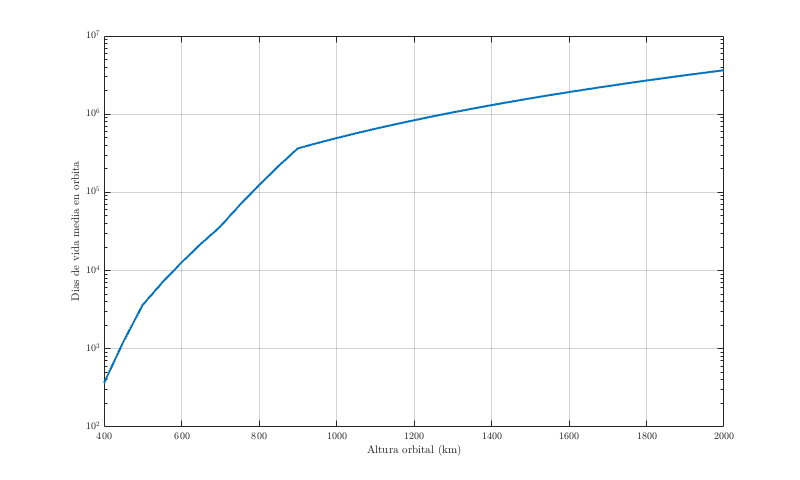
\includegraphics[width=0.9\textwidth]{3.Conceptos_Previos/Diasvidamediaorbitavsaltitud.png} 
    \caption{Días de vida media en órbita vs Altura orbital (km).\\ Fuente: Elaboración propia basada en \cite{spaceacademy_orblife}.}
    \label{fig:vida_media_orbita}
\end{figure}

Los satélites en órbita baja terrestre (LEO), típicamente por debajo de los 1000 km de altitud, están expuestos a una atmósfera tenue pero no nula. A esas alturas, aún existen partículas atmosféricas que ejercen una fuerza de arrastre sobre el satélite a medida que este se desplaza a velocidades orbitales. Este arrastre provoca una pérdida continua de energía orbital,  que hace que el satélite descienda gradualmente a órbitas más bajas. Este fenómeno se conoce como \textbf{decaimiento orbital}.

Con el tiempo, un satélite que no cuenta con sistemas de propulsión para mantener su altitud experimentará una disminución continua de su altura orbital, reingresando eventualmente en la atmósfera densa, donde se desintegrará por el calor generado por la fricción. Este mecanismo actúa también como forma pasiva de mitigación de desechos espaciales, lo cual será interesante tener en consideración una vez llegue el fin de vida del satélite.

\subsection{Radiación Solar}

La radiación solar está compuesta por partículas (fotones) que viajan a la velocidad de la luz. Estos fotones, aunque no tienen masa, sí tienen energía y cantidad de movimiento. 

Cuando los fotones de la radiación solar golpean un objeto, como un satélite, se produce una transferencia de momento del fotón al objeto. Esta pequeña fuerza es la presión de radiación.

Aunque la presión es pequeña, para satélites con grandes superficies expuestas (como los que tienen paneles solares grandes o velas solares), puede producirse una desviación progresiva de la órbita. Puede cambiar el argumento del perigeo, haciendo que la órbita se desplace gradualmente.


\subsection{Problema del tercer cuerpo}

El problema del tercer cuerpo se refiere a la dinámica gravitacional que surge cuando tres objetos celestes (en nuestro caso, el sistema Tierra-Luna- satélite, o Tierra-Sol- satélite) interactúan entre sí mediante la fuerza de gravedad. A diferencia del problema de dos cuerpos, que tiene una solución matemática exacta y predecible, la adición de un tercer cuerpo introduce un nivel de complejidad significativo.

Cuando solo dos cuerpos interactúan gravitacionalmente, sus movimientos forman órbitas estables y predecibles. Sin embargo, cuando se introduce un tercer cuerpo, este genera perturbaciones en las órbitas que serían estables en el caso de dos cuerpos.

El tratamiento analítico de este problema es extraordinariamente difícil porque la perturbación depende explícitamente del tiempo. Las ecuaciones diferenciales que describen este sistema no tienen una solución cerrada o analítica exacta, lo que ha lleva al desarrollo de métodos numéricos para aproximar las soluciones.

El sistema de tres cuerpos es intrínsecamente caótico, lo que significa que es extremadamente sensible a las condiciones iniciales. Pequeñas variaciones en la posición o velocidad inicial de cualquiera de los cuerpos pueden resultar en trayectorias completamente diferentes a largo plazo. Esto imposibilita predicciones precisas sin conocer con exactitud absoluta las condiciones iniciales.\\

\subsection{Órbitas de especial interés}

\subsubsection{Órbitas heliosíncronas}\label{sec:SSO}

Las órbitas heliosíncronas son aquellas en las que el plano orbital mantiene una orientación constante respecto al Sol. Esto permite que el satélite pase sobre cualquier punto de la Tierra a la misma hora solar local, asegurando condiciones de iluminación consistentes para aplicaciones como monitoreo ambiental y teledetección.

El efecto del achatamiento terrestre es clave para lograr esta sincronización. La regresión nodal inducida por el achatamiento puede ajustarse seleccionando adecuadamente la altitud y la inclinación orbital. Para una órbita heliosíncrona, la velocidad angular de precesión del nodo ascendente debe coincidir con la velocidad angular aparente del Sol respecto a la Tierra (\( \approx 0.9856^\circ/\text{día} \)). Con esto se obtiene la ecuación que dará la inclinación de la órbita en función de la altura:

\begin{align}
\cos i = -\frac{2 r^{7/2} \, \omega_{\text{sol}}}{3 J_2 R_T^2 \sqrt{\mu}}
\end{align}

\noindent donde:

\begin{itemize}
    \item \( i \) es la inclinación orbital,
    \item \( r \) es el radio orbital (radio de la Tierra + altitud del satélite),
    \item \( \omega_{\text{sol}} \approx 1.991 \times 10^{-7} \ \text{rad/s} \) es la velocidad angular aparente del Sol respecto a la Tierra,
    \item \( J_2 \approx 1.08263 \times 10^{-3} \) es el coeficiente zonal que representa el achatamiento terrestre,
    \item \( R_T \approx 6378.1 \ \text{km} \) es el radio medio de la Tierra,
    \item \( \mu \approx 3.986 \times 10^{14} \ \text{m}^3/\text{s}^2 \) es la constante gravitacional estándar de la Tierra.
\end{itemize}

\subsubsection{Órbitas de Traza Repetida}


Una órbita de traza repetida (RGT o \textit{Repeating Ground Track}) es aquella en la que el satélite repite su proyección sobre la superficie terrestre después de un número entero de días \( D \) y un número entero de órbitas \( N \). Estas órbitas son especialmente útiles para misiones de observación terrestre, ya que permiten adquirir imágenes de una misma zona bajo condiciones geométricas similares a intervalos regulares.

El criterio para una órbita RGT se establece a partir de la sincronización entre el período orbital \( T_{\mathrm{orb}} \) del satélite y la rotación de la Tierra. La condición matemática que debe cumplirse es:

\begin{equation}
N \cdot T_{\mathrm{orb}} = D \cdot T_{\mathrm{sidereal}}
\end{equation}

donde:
\begin{itemize}
    \item \( N \in \mathbb{N} \): número de órbitas completas en \( D \) días,
    \item \( T_{\mathrm{orb}} \): período orbital del satélite,
    \item \( D \in \mathbb{N} \): número de días (normalmente días solares o sidéreos),
    \item \( T_{\mathrm{sidereal}} = 86164 \, \si{s} \): duración del día sidéreo terrestre.
\end{itemize}


Utilizando la tercera ley de Kepler, se relacionan la altitud orbital y periodo orbital

\begin{equation}
T_{\mathrm{orb}} = 2\pi \sqrt{\frac{(R_T + H)^3}{\mu}}
\end{equation}

De este modo, se obtiene la altitud \( H \) que satisface la condición de repetición. Esta clase de órbitas permite optimizar la planificación de coberturas periódicas.



\subsection{Consideración de las perturbaciones orbitales}


Para el presente trabajo no se considera la radiación solar ni el problema del tercer cuerpo, a fin de simplificar los cálculos necesarios. Esto no es descabellado, ya que, como se verá mas adelante, se evaluará una órbita baja (\textit{Low Earth Orbit}, o LEO ) en la cual la influencia de la gravedad terrestre será en ordenes de magnitud mayores a cualquier otro cuerpo celeste cercano (como la Luna o el Sol). También significa que el telescopio no será excesivamente grande, ni, por ende, el resto de subsistemas, por lo que la fuerza generada por la presión de radiación será de un valor ínfimo. No obstante, esta proximidad a la Tierra hará que la fricción con la atmósfera si sea una perturbación a considerar en el diseño de la misión. Así mismo, el achatamiento terrestre también será fundamental a la hora de considerar órbitas heliosíncronas.

\chapter{Definición del instrumento}
\minitoc

Una vez definidos los fundamentos teóricos que rigen el problema planteado en el presente trabajo, se comienza a definir las variables que cumplan los requisitos impuestos.

Se ha creado para el trabajo un paquete de códigos disponible en el anexo \ref{sec:annexcode} que, en base a los \textit{inputs} iniciales, calcula los requerimientos y exporta las soluciones óptimas listas a interpretar por el usuario. El código maestro, que aloja dichos parámetros de entrada y las llamadas a las funciones, alberga el siguiente flujo de trabajo:

\begin{landscape}
    

\begin{figure}[H]
    \centering
    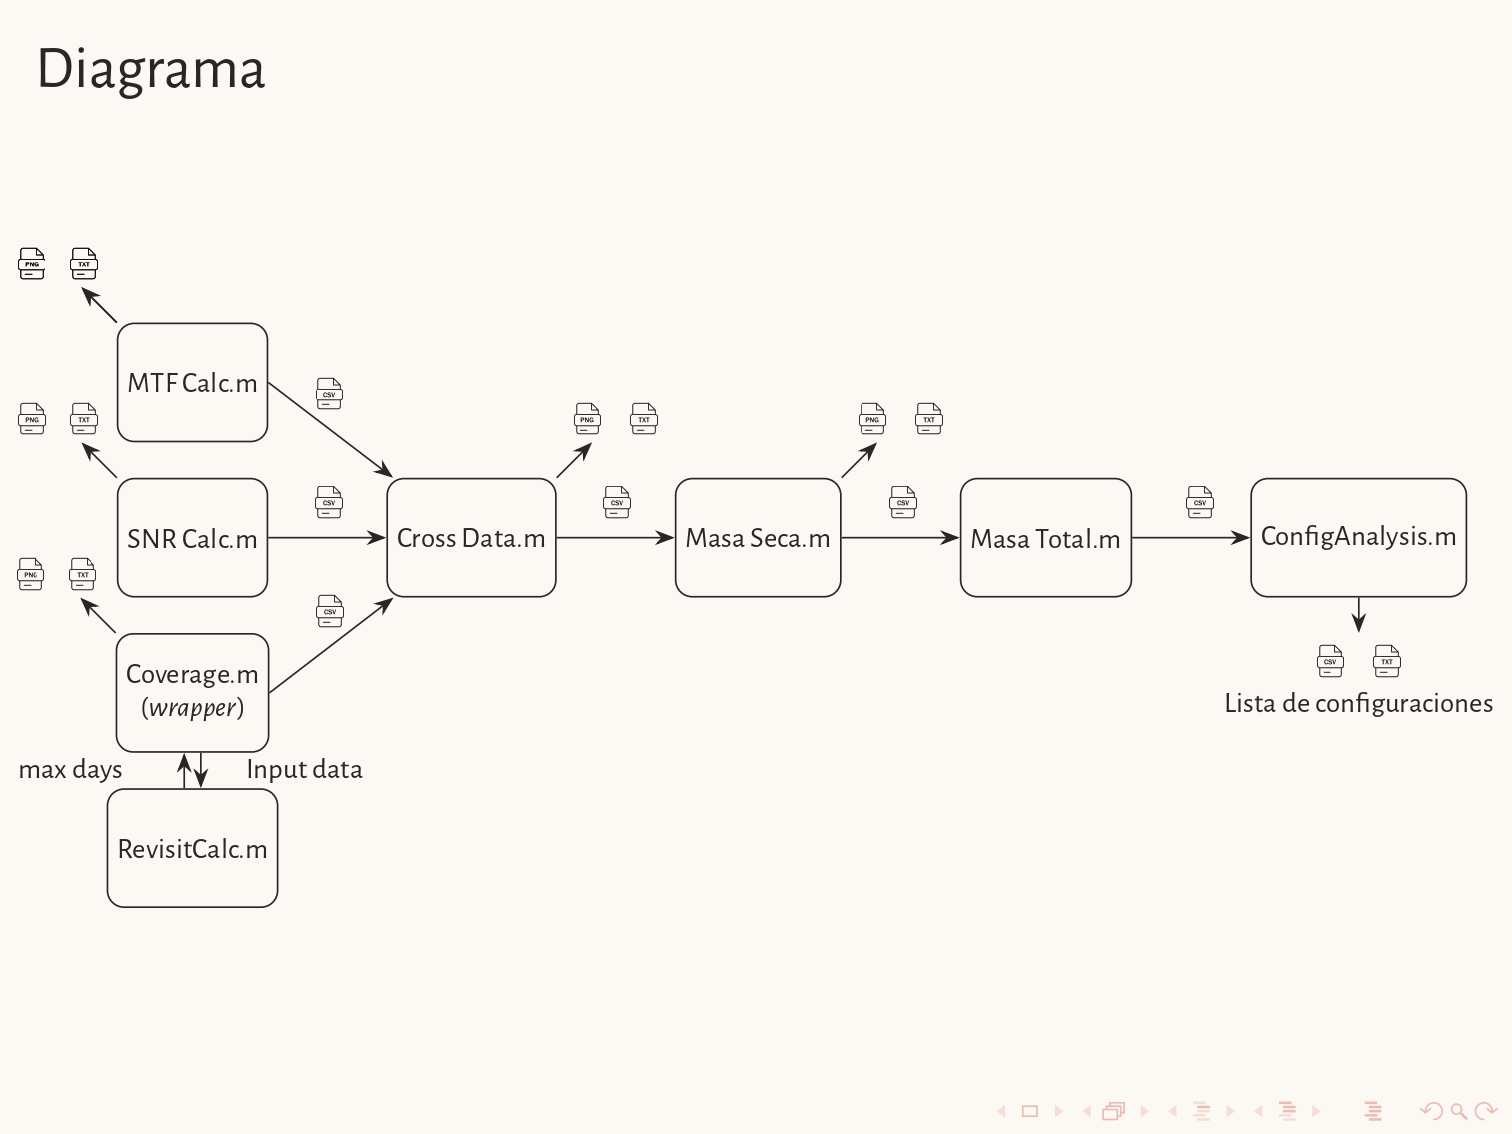
\includegraphics[width=1\linewidth]{4.Payload/workflow.jpg}
    \caption{Flujo de trabajo de los scripts de MATLAB}
    \label{fig:flowchart}
\end{figure}
\end{landscape}
\newpage

\section{GSD}

Se comenzará por definir el GSD, ya que es un parámetro que implícitamente viene dado por las condiciones del cliente. Según el requerimiento debemos ser capaces de poder diferenciar fuentes puntuales de CO2 en las ciudades estadounidenses.

Primeramente se extrae una imagen satélite del cinturón industrial de Houston para escoger de una manera mas visual la selección de GSD. Mediante el software \textit{open source} GIMP se puede pixelar esta imagen para visualizar la elección del GSD. Dicha foto tiene 1673 pixeles de ancho, y mediante el software Google Earth, proporciona el dato del ancho de la imagen en la realidad, correspondiente a 14251 m. Por tanto, el GSD de esta captura será: 

\begin{equation}
\frac{14251\ m}{1673\ pix} \approx 8.516
\end{equation}


\begin{figure}[H]
    \centering
    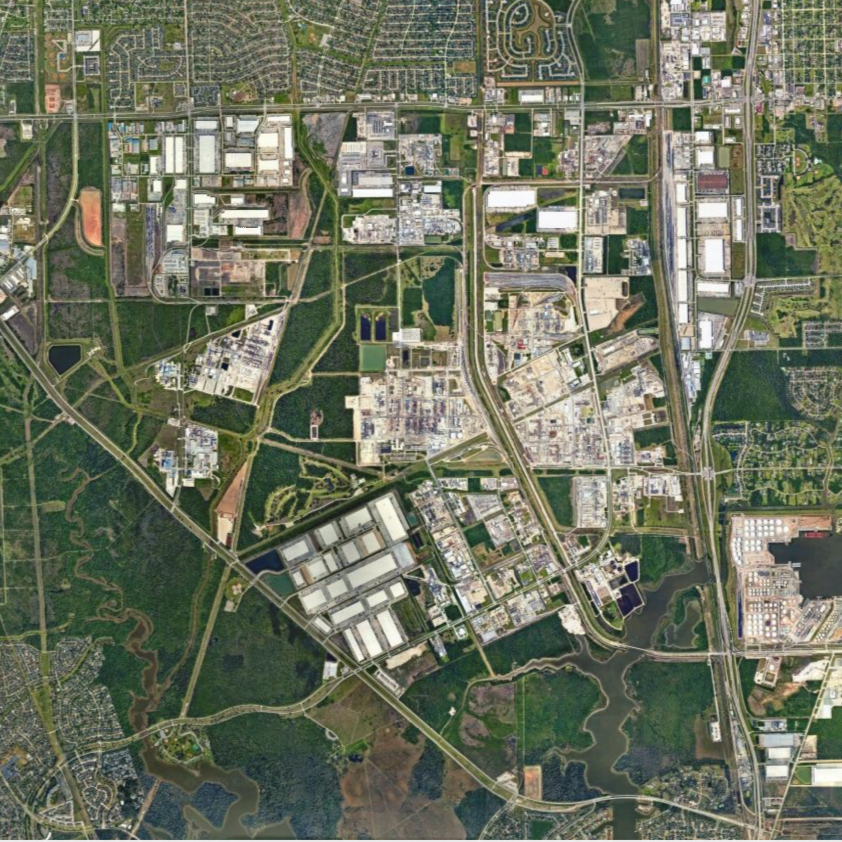
\includegraphics[width=0.7\textwidth]{4.Payload/Houston.jpg}
    \caption{Imagen satélite del cinturón industrial de Houston. $GSD \approx 8,5$. \\ Fuente: Google Earth (29°42'18.0"N; 95°00'10.8"W)}
    \label{fig:Houston}
\end{figure}

Esta resolución resulta excesiva para las especificaciones del proyecto, ya que permite observar las instalaciones industriales con gran detalle. Se puede sacrificar este parámetro en favor del resto de variables a seleccionar. Un análisis comparativo con diferentes valores de GSD demuestra que una resolución de \textbf{80 metros} permite diferenciar edificios industriales entre sí y distinguirlos de las zonas residenciales, cumpliendo así con los requerimientos de precisión del cliente.

\begin{figure}[H]
    \centering

    % Primera fila
    \begin{subfigure}[b]{0.3\textwidth}
        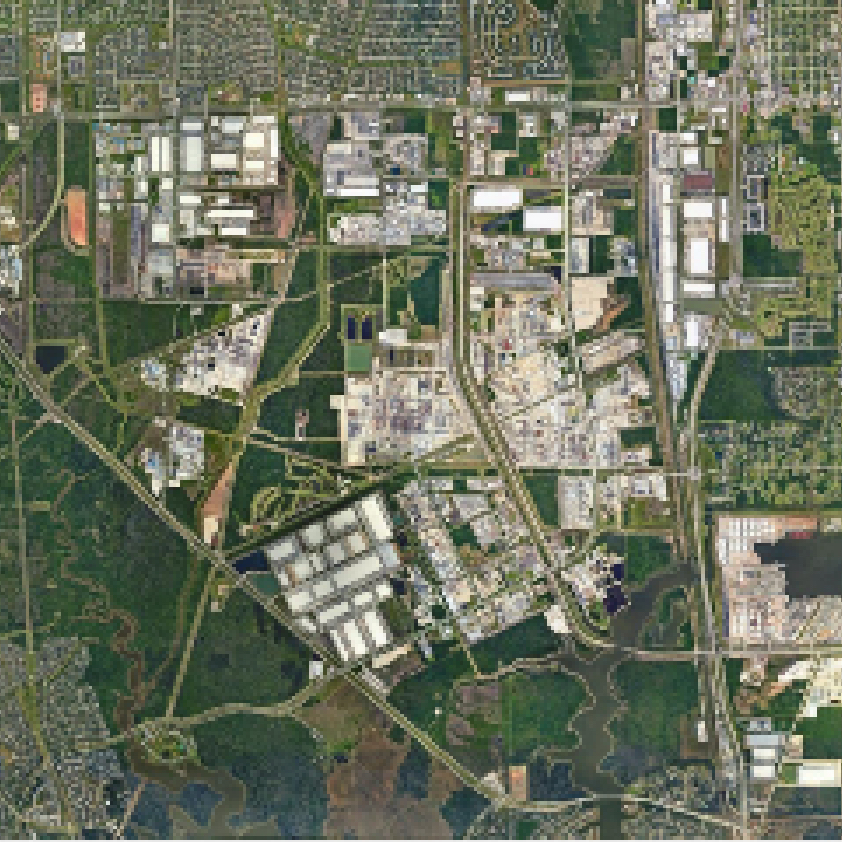
\includegraphics[width=\textwidth]{4.Payload/Houston GSD 30.jpg}
        \subcaption{GSD 30}
    \end{subfigure}
    \hfill
    \begin{subfigure}[b]{0.3\textwidth}
        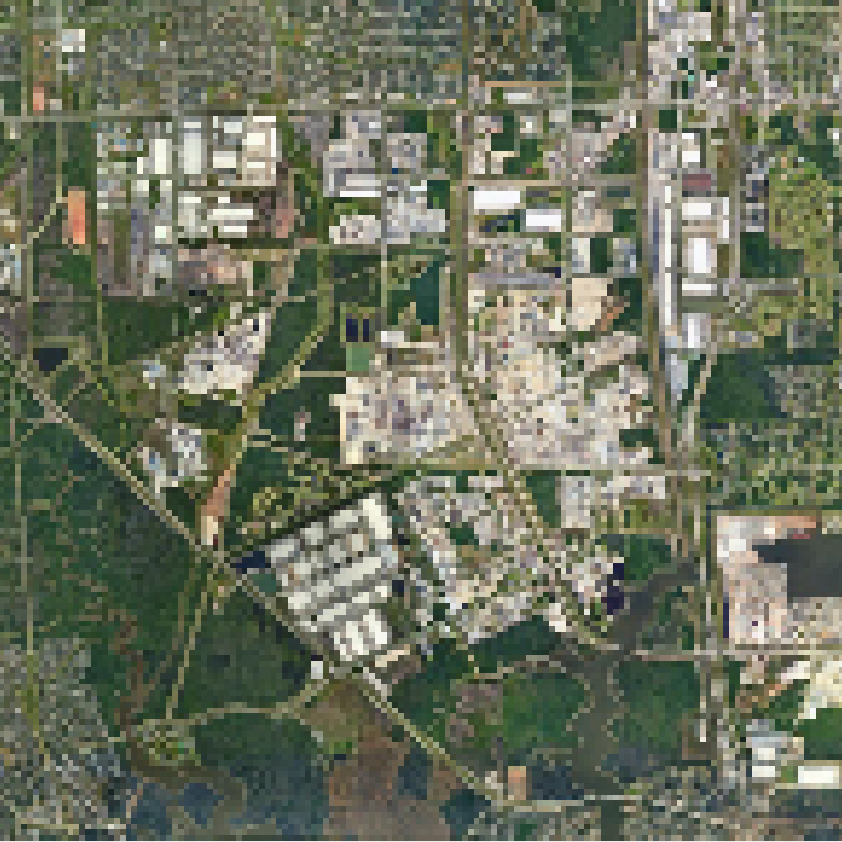
\includegraphics[width=\textwidth]{4.Payload/HoustonGSD50.jpg}
        \subcaption{GSD 50}
    \end{subfigure}
    \hfill
    \begin{subfigure}[b]{0.3\textwidth}
        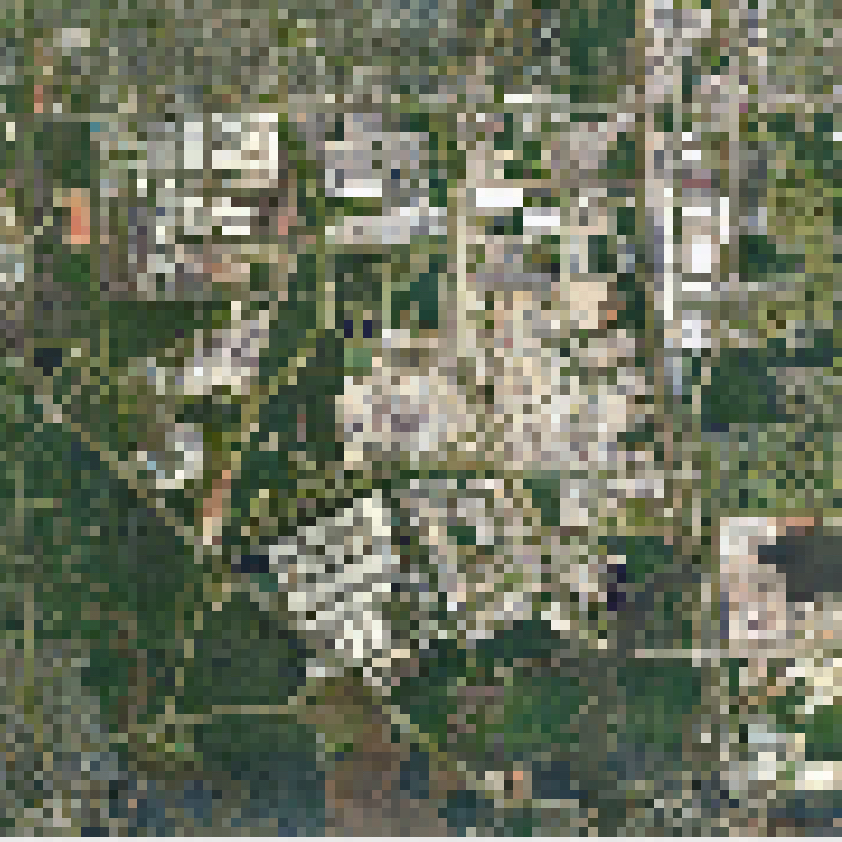
\includegraphics[width=\textwidth]{4.Payload/HoustonGSD80.jpg}
        \subcaption{GSD 80}
    \end{subfigure}

    \vspace{1em}

    % Segunda fila
    \begin{subfigure}[b]{0.3\textwidth}
        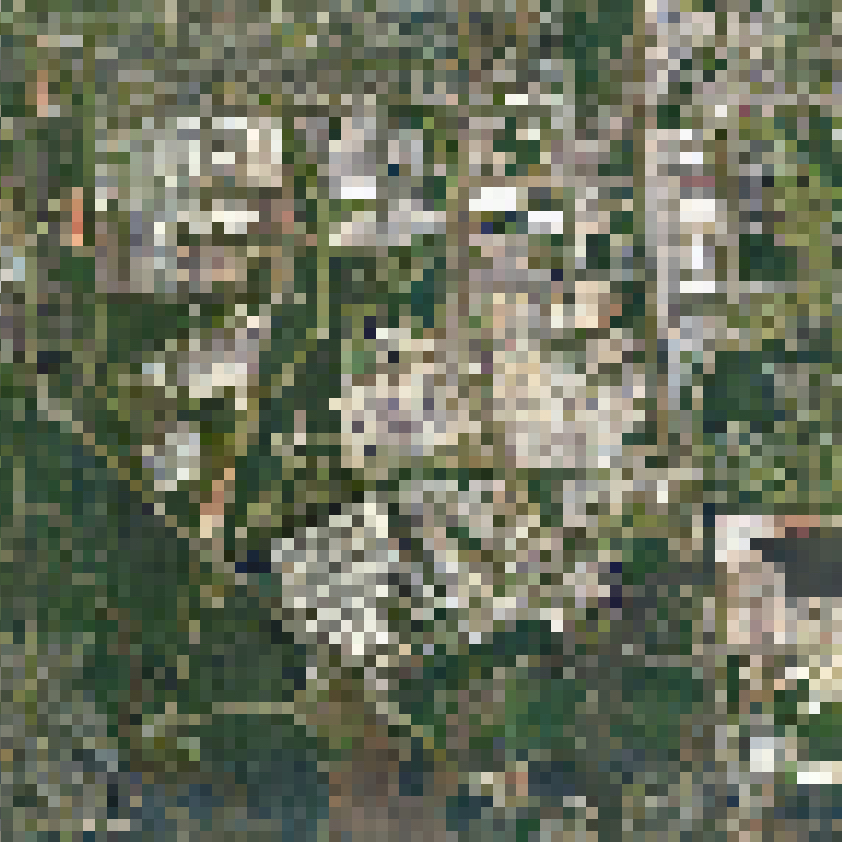
\includegraphics[width=\textwidth]{4.Payload/HoustonGSD100.jpg}
        \subcaption{GSD 100}
    \end{subfigure}
    \hfill
    \begin{subfigure}[b]{0.3\textwidth}
        
\includegraphics[width=\textwidth]{4.Payload/Houston GSD150.jpg}
        \subcaption{GSD 150}
    \end{subfigure}
    \hfill
    \begin{subfigure}[b]{0.3\textwidth}
        
\includegraphics[width=\textwidth]{4.Payload/Houston GSD200.jpg}
        \subcaption{GSD 200}
    \end{subfigure}

    \caption{Comparación de imágenes con distintas condiciones de GSD. \\Fuente: Imagen adaptada, Google Earth.}
    \label{fig:comparacion_gsd}
\end{figure}


\section{Bandas espectrales. Ancho de banda} \label{sec:specbands}

La selección de bandas espectrales se fundamenta en las características de absorción del CO\textsubscript{2} y los requisitos de calibración atmosférica necesarios para garantizar la precisión de las mediciones.

\subsubsection{Banda O\textsubscript{2} A-Band (0,76 \textmu m)}

La banda de absorción del oxígeno atmosférico a 0,76 \textmu m se emplea para la calibración de la columna de aire. El oxígeno presenta una concentración atmosférica estable y conocida (20,95\%), lo que permite determinar con precisión la masa de aire atravesada por la radiación solar. Esta referencia resulta esencial para normalizar las mediciones de CO\textsubscript{2} y corregir variaciones debidas a diferencias en el camino óptico atmosférico.

\subsubsection{Bandas CO\textsubscript{2} SWIR (1,61 y 2,06 \textmu m)}

Las bandas de 1610 nm y 2060 nm corresponden a las principales regiones de absorción del CO\textsubscript{2} en el infrarrojo de onda corta, como se vio en el capítulo \ref{cap3}. La utilización de dos bandas independientes permite implementar algoritmos de validación cruzada y mejora el calculo de estimaciones de concentración.

\subsubsection{Ancho de banda}

En cuanto al ancho de banda espectral, se ha seleccionado un valor de 20 nm para todas las bandas. Esta elección representa un equilibrio entre la resolución espectral y la relación señal-ruido, permitiendo aislar adecuadamente las características de absorción objetivo sin comprometer la sensibilidad del sistema. Un ancho de banda más estrecho proporcionaría mayor especificidad espectral, pero reduciría la cantidad de fotones detectados y, por tanto, la SNR. Por el contrario, un ancho de banda excesivamente amplio dificultaría la discriminación de las líneas de absorción. El valor adoptado se encuentra dentro de los estándares habituales en instrumentación óptica para aplicaciones de teledetección y garantiza el cumplimiento de los requisitos de precisión y robustez en la recuperación de concentraciones de CO\textsubscript{2} y parámetros atmosféricos \cite{skoog2017principles,}.
\\

\begin{table}[h]
\centering
\caption{Bandas espectrales elegidas.}
\begin{tabular}{l c c l}
\toprule
\textbf{Banda} & \textbf{$\lambda$ (\textmu m)} & \textbf{$\Delta\lambda$ (nm)} & \textbf{Propósito principal} \\
\midrule
O$_2$ A-Band       & 0,76  & 20    & Calibración columna aire \\
CO$_2$ SWIR 1      & 1,61  & 20    & Absorción principal de CO$_2$ \\
CO$_2$ SWIR 2      & 2,06  & 20    & Absorción secundaria de CO$_2$ \\
\bottomrule
\end{tabular}

\label{tab:banda_propósitos}
\end{table}



\section{Detectores, filtros y escaneo}



\subsection{Elección de detectores}

Una vez definidas las bandas de interés se procederá a buscar el detector que sea capaz de cubrir dichos rangos de detección para la misión. Para ello, se elabora una lista de detectores disponibles en mercado de los cuales se escogerán mas adelante, el más apropiado según sus especificaciones. Para las bandas 1,61 \textmu m y 2,01 \textmu m se evaluaran los siguientes detectores:

%% TABLA
\begin{table}[H]
\centering
\caption{Comparación de características de detectores SWIR}
\begin{tabular}{lccc}
\toprule
& \textbf{Detector 1} \cite{lynred_capyork} & \textbf{Detector 2} \cite{teledyne_hawaii2rg} & \textbf{Detector 3} \cite{sofradir_saturn_visir_2011}\\
\midrule
\textbf{Nombre} & LYNRED CAPYORK  & Teledyne H2RG   & Saturn VISIR \\
\textbf{Tamaño pixel} & 15 x 15 \textmu m & 18 × 18 \textmu m & 30 × 30 \textmu m \\
\textbf{Array} & 1200 × 12 & 2048 × 2048 &  1000 × 256 \\
\textbf{Canales\tablefootnote{Evaluar los canales de salida permite evaluar cuantas bandas independientes es capaz de capturar un detector}} & 4 & 4 & 4 ó 8 \\
\textbf{TDI} & Si (4 etapas) & No  & No \\
\textbf{Rango espectral} & 0,8-5 \textmu m & 0,4-2,5 \textmu m & 0,3-2,5 \textmu m \\
\textbf{Eficiencia cuántica} & 85\% &  70\% &  70\%  \\
\textbf{MTF @ Nyquist} & 0,45  & 0,5 & 0,48 \\
\bottomrule
\end{tabular}

\label{tab:detectores_comparacion}
\end{table}

Se aprecia que los detectores 2 y 3 tienen un rango válido para evaluarse también en la banda 0,76 \textmu m, mientras que el Detector CAPYORK será incapaz de recepcionar datos en esta banda. Por ello, para la banda O\textsubscript{2} se evaluarán, además de los detectores 2 y 3, un detector adicional que complemente al LYNRED CAPYORK. Resulta el CMOS STAR250 una opción a evaluar: 

%% TABLA

\begin{table}[H]
\centering
\caption{Comparación de características de detectores para \textit{A-Band} O\textsubscript{2}.}
\label{tab:detectores_comparacion_2}
\begin{tabular}{lccc}
\toprule
& \textbf{Detector 4} \cite{cypress_star250_2009}  & \textbf{Detector 5}\cite{teledyne_hawaii2rg} & \textbf{Detector 6} \cite{sofradir_saturn_visir_2011} \\
\midrule
\textbf{Nombre} & STAR250 & Teledyne H2RG & SATURN VISIR \\
\textbf{Tamaño pixel} & 25 × 25 \textmu m & 18 × 18 \textmu m & 30 × 30 \textmu m \\
\textbf{Array} & 512 × 512 & 2048 × 2048 & 1000 × 256 \\
\textbf{Canales} & 4 & 4 & 4 ó 8 \\
\textbf{TDI} & No & No  & No  \\
\textbf{Rango espectral} & 0,4–1,1 \textmu m & 0,4–2,5 \textmu m & 0,3 –2,5 \textmu m \\
\textbf{Eficiencia cuántica} & 35 \% &  70\% &  50\% \tablefootnote{Según especificaciones del fabricante; desciende un 20\% para rango visible} \\
\textbf{MTF @ Nyquist} & 0,36 & 0,5 & 0,45 \\
\bottomrule
\end{tabular}

\end{table}


Más adelante se determinará el número de detectores a utilizar, así como su disposición, ya que se debe trabajar con un \textit{swath} mínimo para asegurar cobertura.


\subsection{Método de escaneo}

El escaneo \textbf{\textit{pushbroom}} se elige sobre alternativas como \textit{whiskbroom} o \textit{step and stare} por su fiabilidad, simplicidad mecánica y optimización de la relación señal-ruido. A diferencia del \textit{whiskbroom}, que utiliza espejos oscilantes para barrer transversalmente la franja de observación, el \textit{pushbroom} emplea un array lineal de detectores fijos que captura toda la franja simultáneamente. Esto elimina componentes mecánicos, reduce el riesgo de desgaste y simplifica el diseño.

Además, el \textit{pushbroom} ofrece un mayor tiempo de integración por píxel, lo que incrementa la SNR al permitir que los detectores acumulen más fotones. En comparación, el \textit{step and stare} limita la cobertura continua y exige maniobras satelitales complejas, añadiendo dificultad a las operaciones de mantenimiento en orbita, incrementando el peso para el control de actitud y limitando el tiempo de revisita.

\subsection{Eleccion de filtros}

Se escogen filtros \textit{\textbf{microstrip}} integrados en el mismo detector. La principal ventaja de los filtros microstrip frente a alternativas como la rueda de filtros reside en su baja masa y fiabilidad mecánica, ya que carecen completamente de partes móviles que pudieran fallar durante los 8 años de misión. Esta característica es crucial considerando el entorno espacial con sus ciclos térmicos extremos y vibraciones durante el lanzamiento. Además, permiten la adquisición simultánea de todas las bandas espectrales necesarias, lo que resulta fundamental para asegurar la correcta corregistración espacial de los datos.


Desde el punto de vista óptico, los filtros microstrip pueden optimizarse individualmente para cada banda espectral, permitiendo un ajuste fino del ancho de banda.


La implementación práctica implicaría fabricar filtros de interferencia multicapa específicamente diseñados para cada banda y detector, con materiales optimizados según el rango espectral (dieléctricos para visible/NIR, y compuestos especiales para SWIR). Estos se montarían directamente sobre cada array de detectores, lo que también minimiza el tamaño del instrumento al evitar mecanismos adicionales \cite{macleod2010}.

\section{Tipo de órbita. Altura orbital. Hora de paso local}

Como se ha expuesto en el capítulo \ref{semejantes}, las misiones de observación terrestre con requerimientos comparables adoptan, de manera unánime, \textbf{órbitas heliosíncronas}. Esta elección responde a la necesidad de garantizar condiciones de iluminación solar consistentes, ya que los detectores empleados dependen de la radiación solar para captar adecuadamente la señal reflejada desde la superficie terrestre.


Una limitación inherente a estos sistemas es su incapacidad para operar eficazmente en condiciones de penumbra. Por tanto, resulta esencial que la trayectoria orbital proporcione una iluminación solar directa y estable en cada pasada del satélite. La órbita heliosíncrona cumple precisamente este requisito, ya que su precesión mantiene el ángulo entre el plano orbital y el Sol constante a lo largo del año, asegurando que cada observación sobre una misma región se realice a una hora solar local fija. Esta estabilidad favorece la coherencia radiométrica de las imágenes y mejora la comparabilidad temporal de los datos adquiridos. Por ello se computarán soluciones de órbita \textbf{heliosíncrona entre los 350 km y los 1400 km de altitud}, con un discretización de 10 km de paso \cite{nasa_sso_slots_2011}.

Otras opciones de órbita compatibles con el requerimiento de iluminación podrían ser órbitas geoestacionarias o una constelación en orbitas Molniya. Estas no son consideradas en el trabajo, pues las alturas necesarias para este tipo de configuración orbital obliga a instalar diámetros de pupila mucho mayores a las requeridas en satélites en órbita LEO, aumentando el peso, el delta-V requerido para la inyección y por ende, el coste total de la misión.

Para la presente misión se ha seleccionado una \textbf{hora de paso ascendente local (LTAN) de 06:00}, lo que proporciona una configuración \textit{Dawn-Dusk}. En este tipo de órbita, el satélite cruza el ecuador terrestre cerca de la línea del línea crepuscular, donde la transición entre el día y la noche es continua. Esta disposición asegura que el satélite permanezca próximo al límite entre la zona iluminada y la zona en sombra de la Tierra, evitando así la entrada en el cono de sombra terrestre y garantizando la exposición solar durante toda la órbita. Como resultado, se obtienen condiciones de iluminación homogéneas tanto en las pasadas ascendentes como en las descendentes, maximizando las pasadas útiles\cite{Boain2004}.

\section{Cálculo de la MTF}

Con la base teórica definida en al apartado \ref{sec:MTFteoria}, así como las especificaciones de los detectores y telescopios a evaluar, se procede a computar en función de la altura orbital y el diámetro de pupila, mediante un script de MATLAB, los valores de MTF totales de la instrumentación óptica. La discretización del diámetro de pupila será de un paso de 1 mm.

Los valores a usar para la computación son:

\begin{table}[H]
\centering
\caption{Parámetros iniciales para el calculo de MTF. \\ Fuente: \cite{zorita_mtf_2023}.}
\begin{tabular}{l r}
\hline
\textbf{Parámetro} & \textbf{Valor} \\
\hline
MTF aberraciones & 0,95 \\
MTF fabricación & 0,98 \\
MTF vibraciones & 0,99 \\
MTF termoelástico & 0,95 \\
MTF Margen & 10\% \\
\hline
\end{tabular}

\end{table}

Dado que el proyecto se encuentra en una etapa temprana de diseño, se establece un margen del 10\% en el cálculo con el fin de cubrir posibles desviaciones asociadas a incertidumbres en los parámetros de entrada, tolerancias de fabricación, o variaciones operacionales. Este margen permite mantener una estimación conservadora sin comprometer la viabilidad preliminar del sistema.

Mediante un análisis dimensional, puede demostrarse que la función de transferencia de modulación (MTF, por sus siglas en inglés) es inversamente proporcional a la longitud de onda $\lambda$. Al aumentar $\lambda$, disminuye la frecuencia de corte $f_{co}$ y, en consecuencia, la capacidad del sistema para transmitir detalles de alta frecuencia espacial se ve reducida.

Por lo tanto, la banda más restrictiva corresponde a la mayor longitud de onda considerada. En el presente caso, para $\lambda = 2{,}01\,\mu\text{m}$, se obtiene la frecuencia de corte más baja y, por ende, la MTF más limitada, con lo que solo se presentan los datos de dicha banda. El resto de los datos se pueden encontrar en el anexo A. Así, junto con los valores de MTF de los detectores en la tabla \ref{tab:detectores_comparacion} y los valores de MTF de alineamiento de los telescopios de la tabla \ref{tab:tabla_telescopios}, se obtienen los siguientes resultados:

%% TABLAS MTF

%% Lambda 2
\begin{landscape}
\begin{figure}[p]
\centering
\setlength{\tabcolsep}{2pt}
\renewcommand{\arraystretch}{0}

\begin{tabular}{cc}
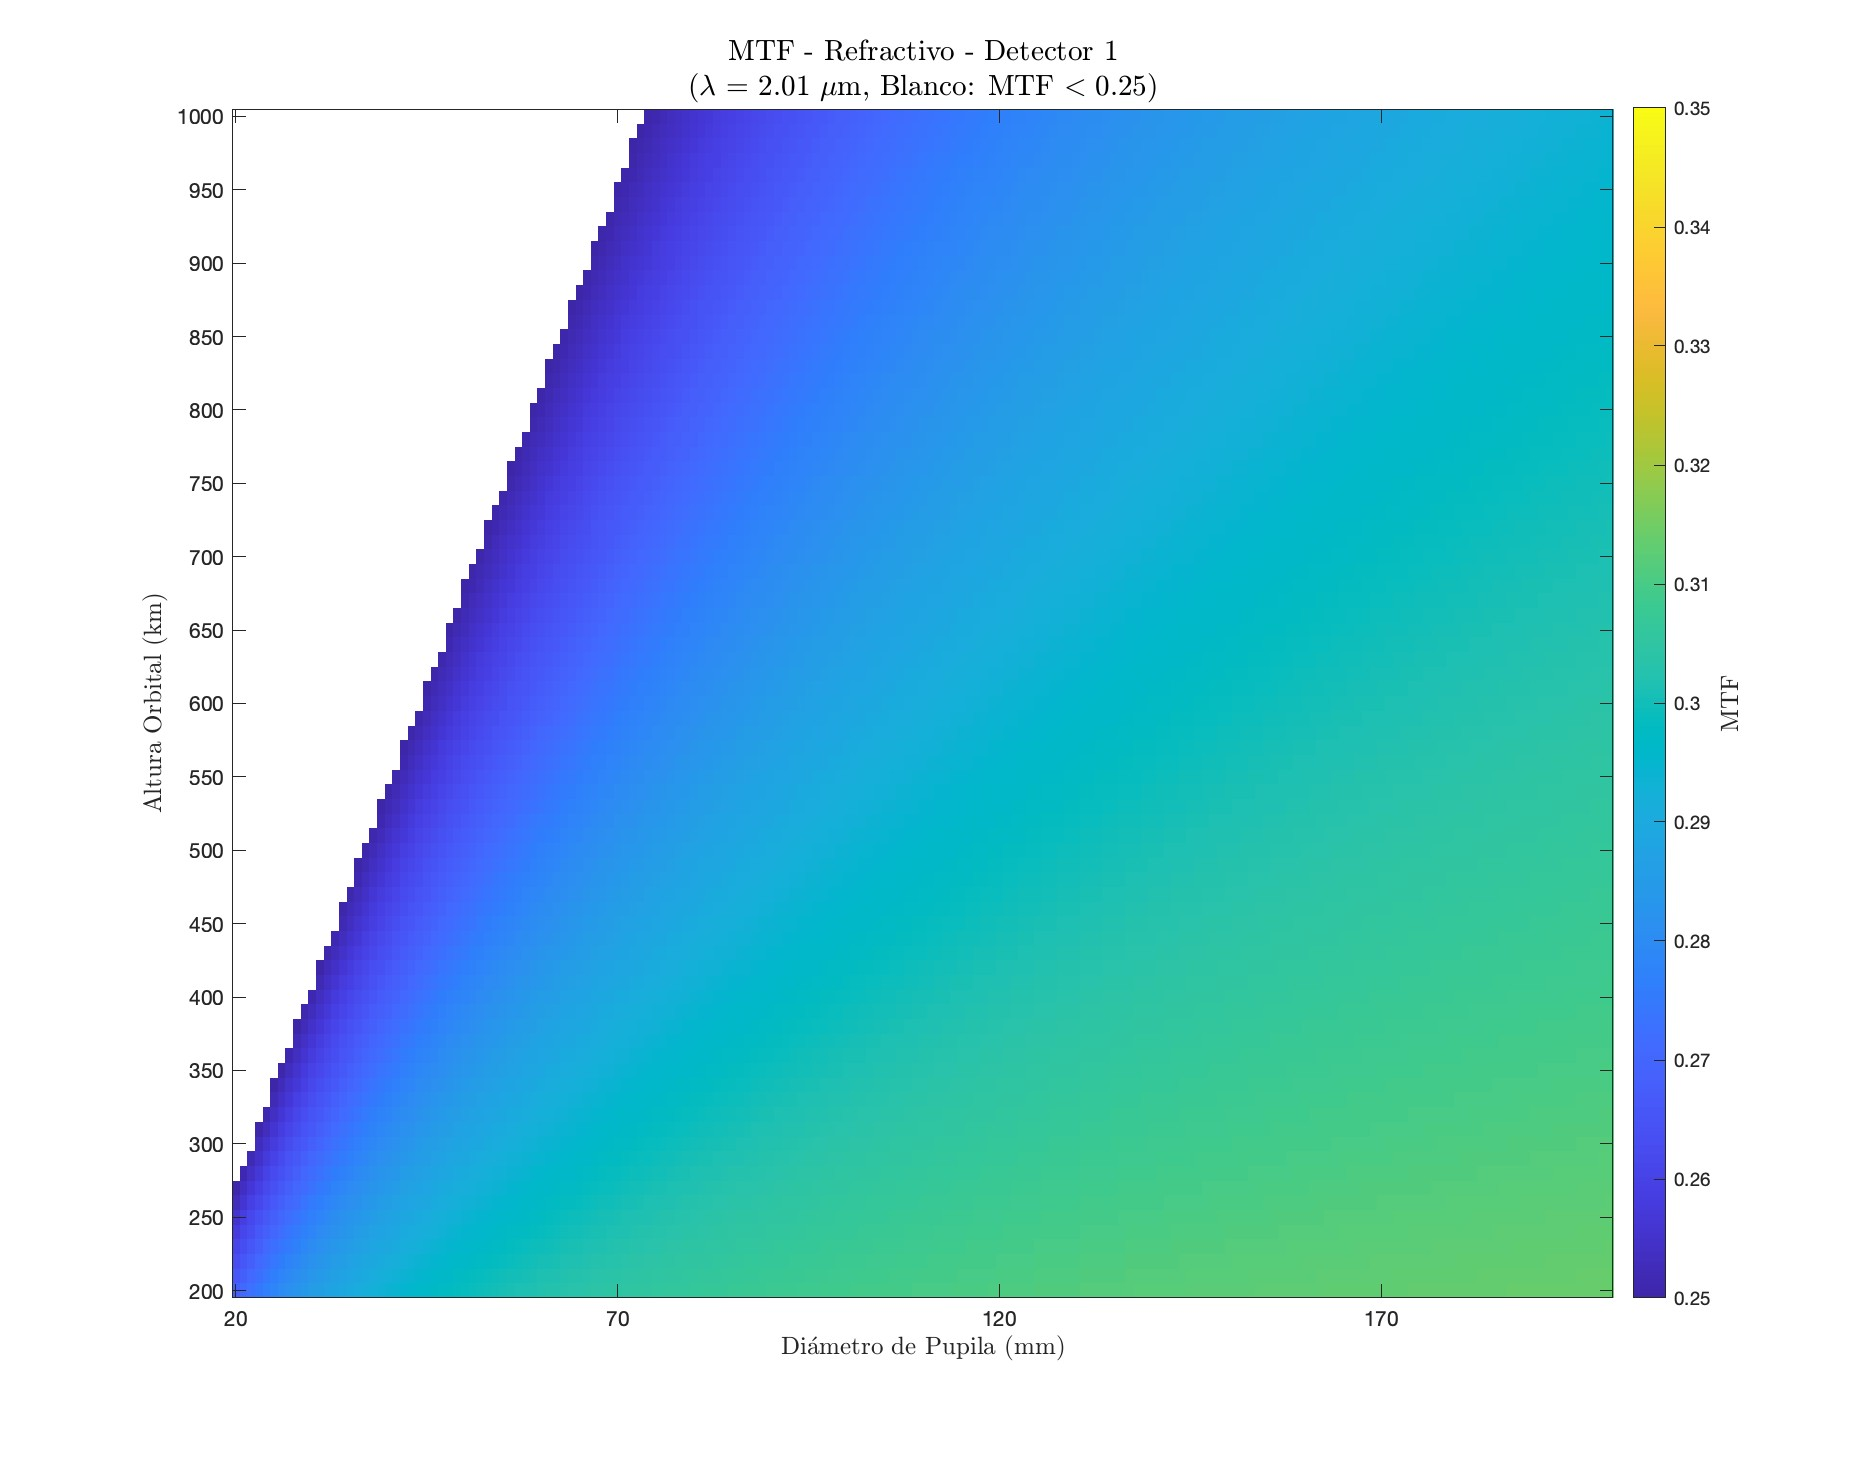
\includegraphics[width=0.48\linewidth]{4.Payload/MTF/MTF_Lambda2_Detector1_Telescopio1_heatmap.jpg} &
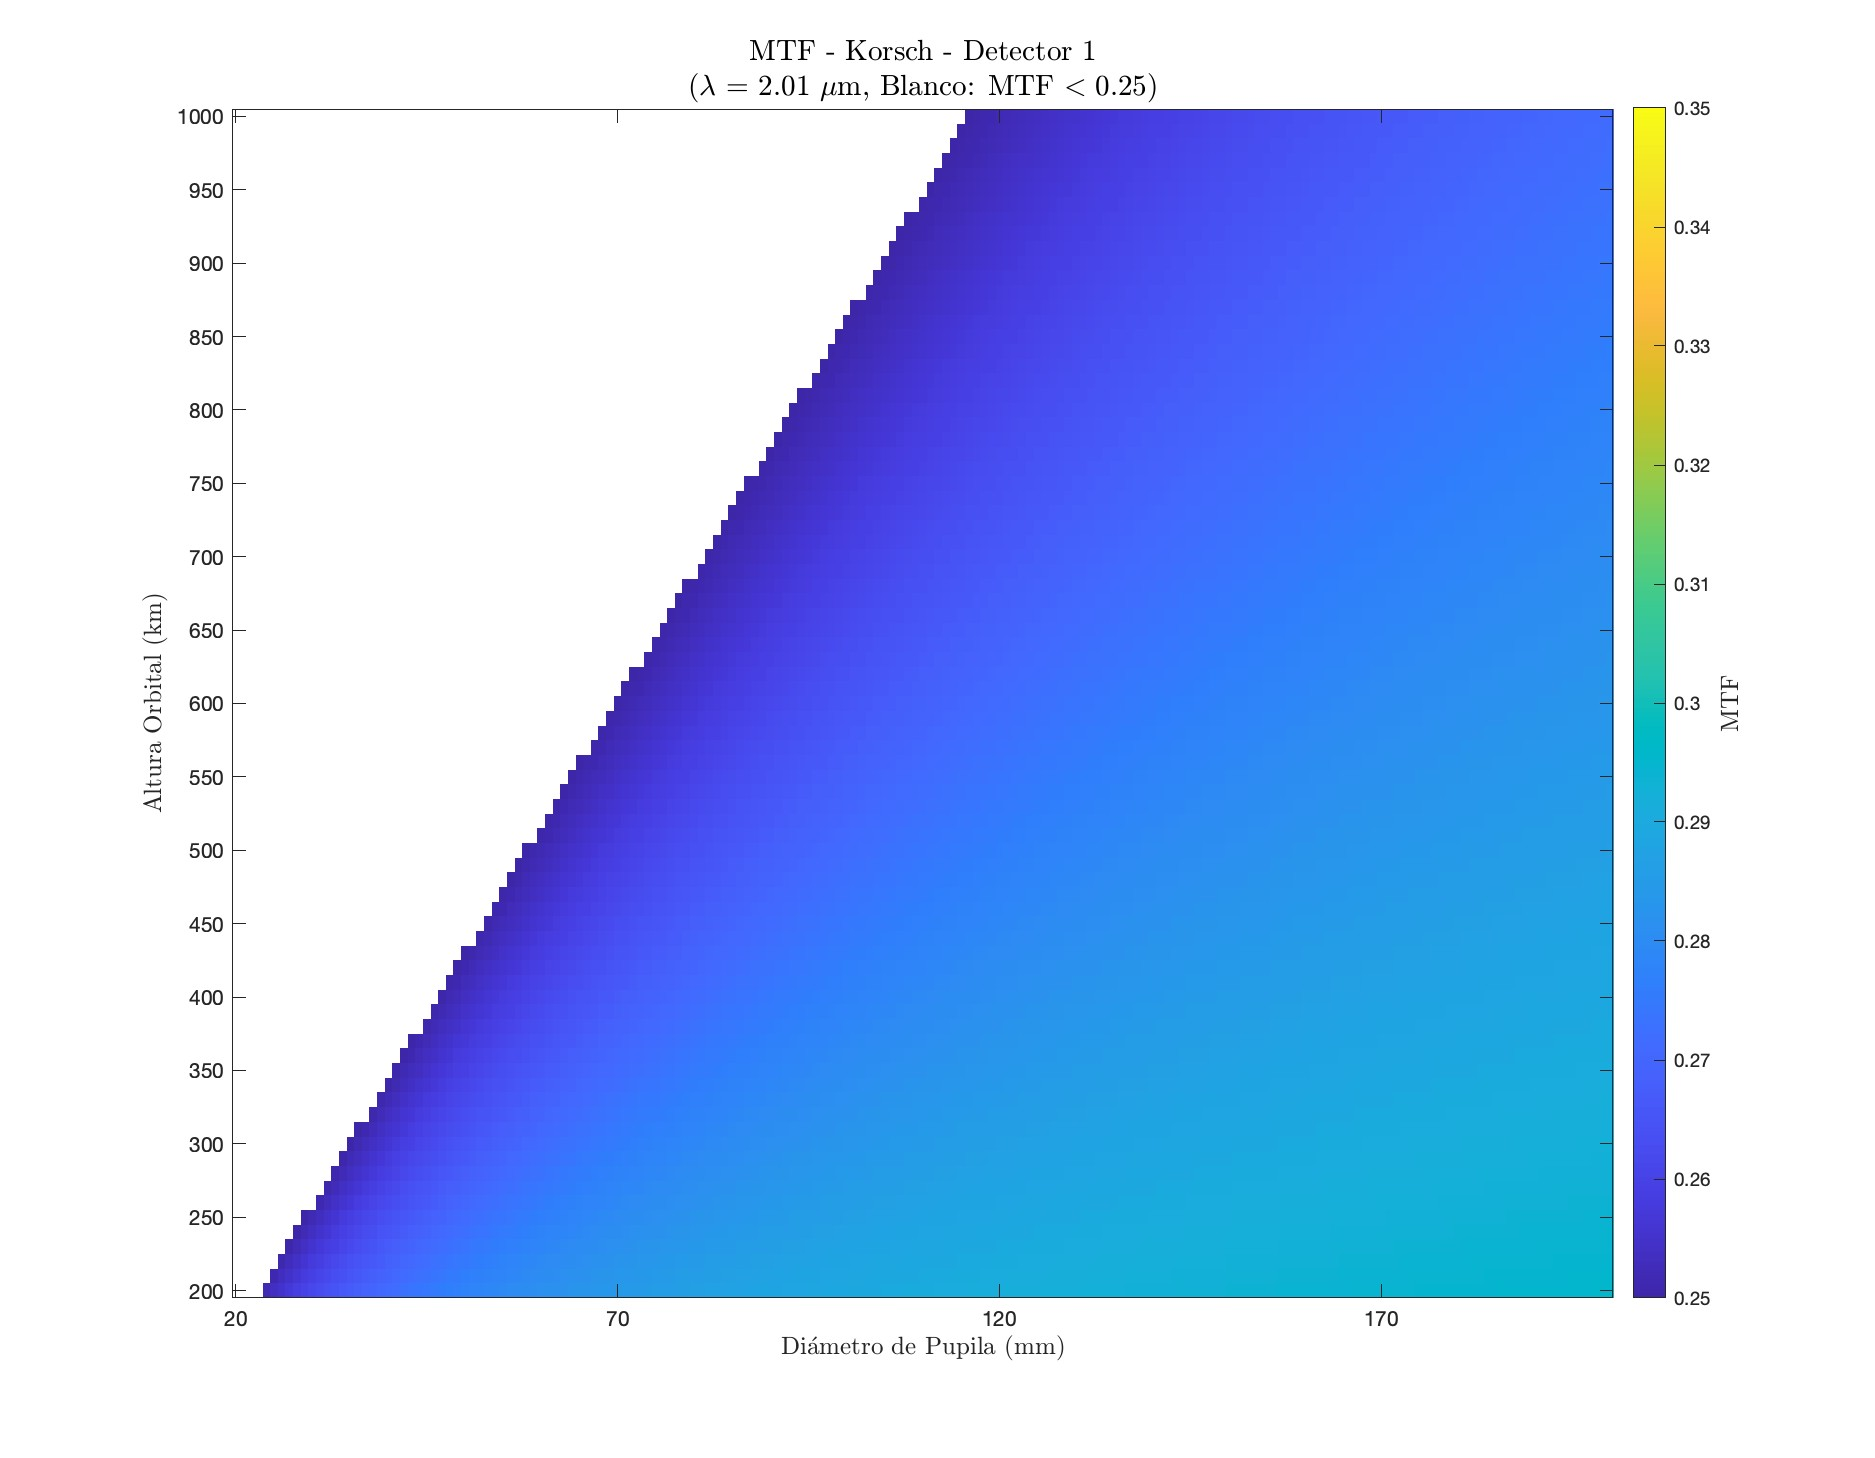
\includegraphics[width=0.48\linewidth]{4.Payload/MTF/MTF_Lambda2_Detector1_Telescopio2_heatmap.jpg} \\
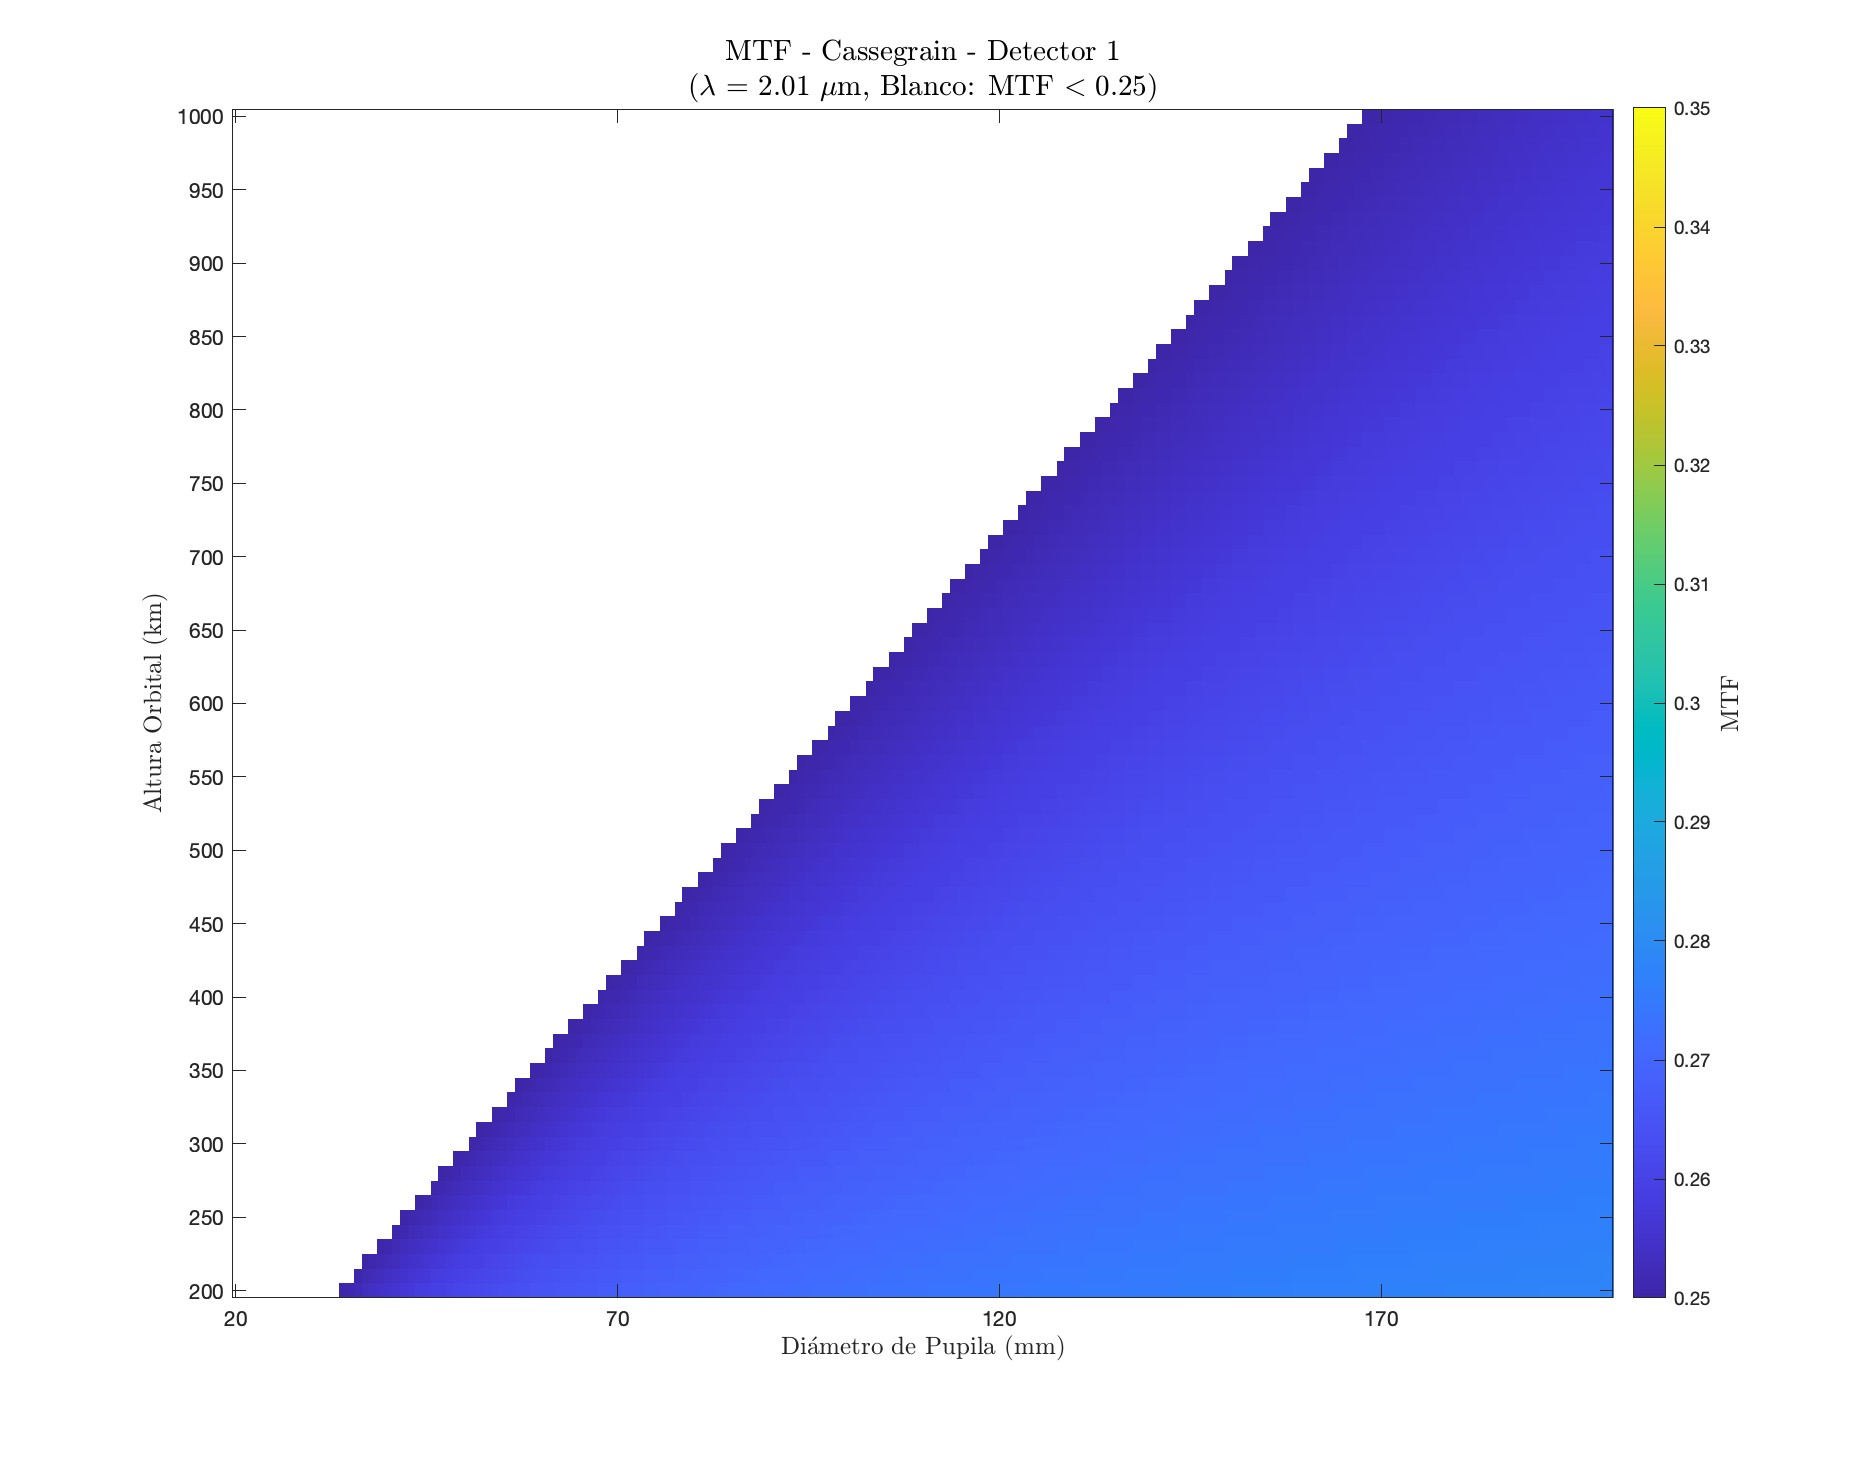
\includegraphics[width=0.48\linewidth]{4.Payload/MTF/MTF_Lambda2_Detector1_Telescopio3_heatmap.jpg} &
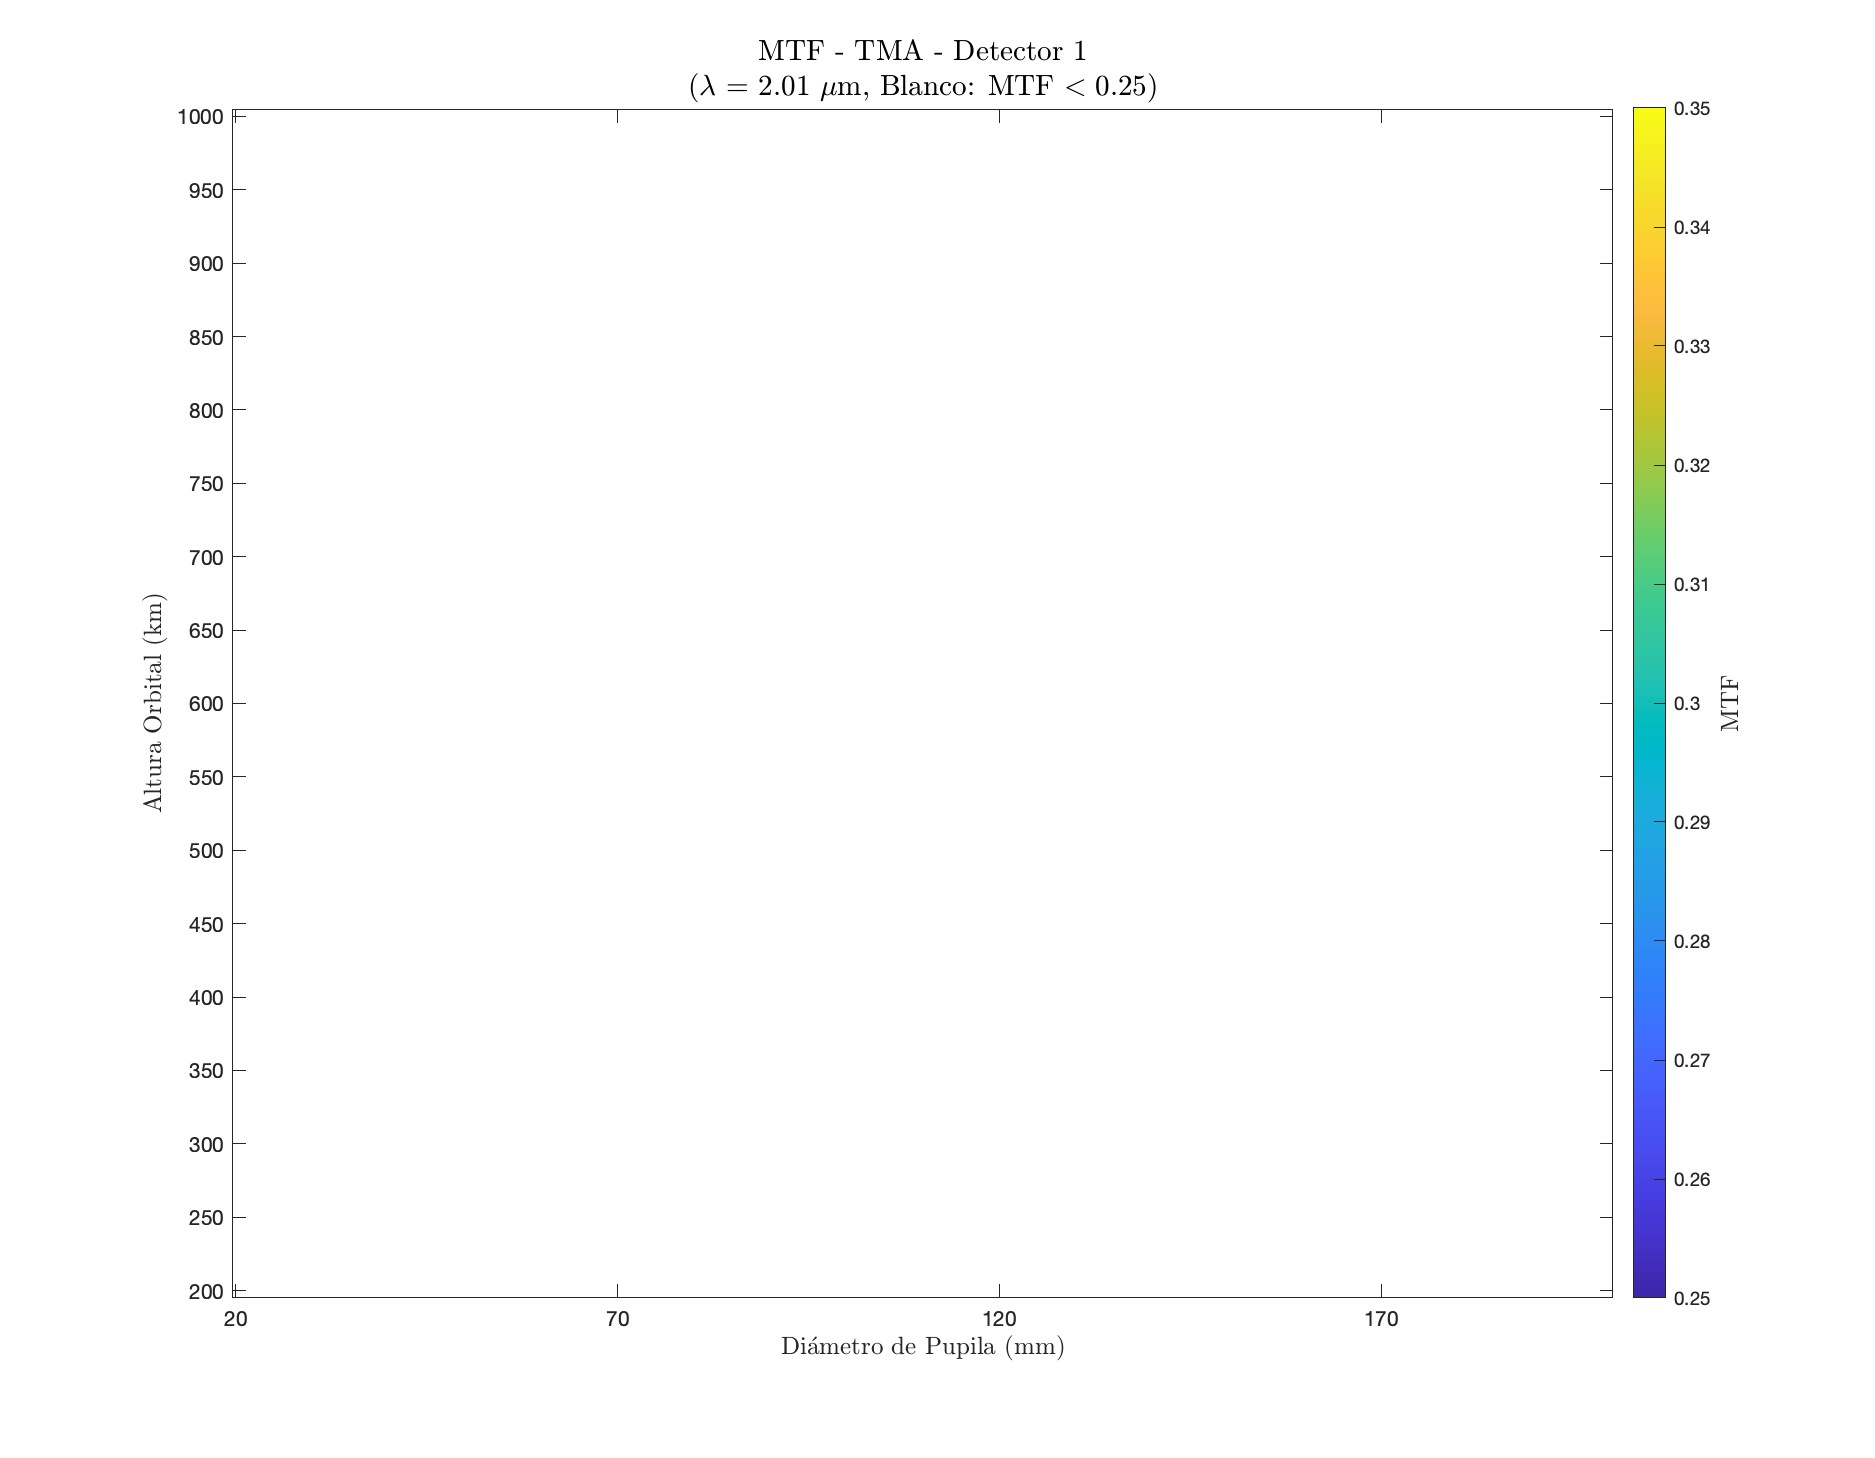
\includegraphics[width=0.48\linewidth]{4.Payload/MTF/MTF_Lambda2_Detector1_Telescopio4_heatmap.jpg} \\
\end{tabular}
\caption{Mapas de calor resultantes del calculo de MTF: Banda 2,01 \textmu m; Detector 1}
\end{figure}
\end{landscape}


%% DETECTOR 2
\begin{landscape}
\begin{figure}[p]
\centering
\setlength{\tabcolsep}{2pt}
\renewcommand{\arraystretch}{0}

\begin{tabular}{cc}
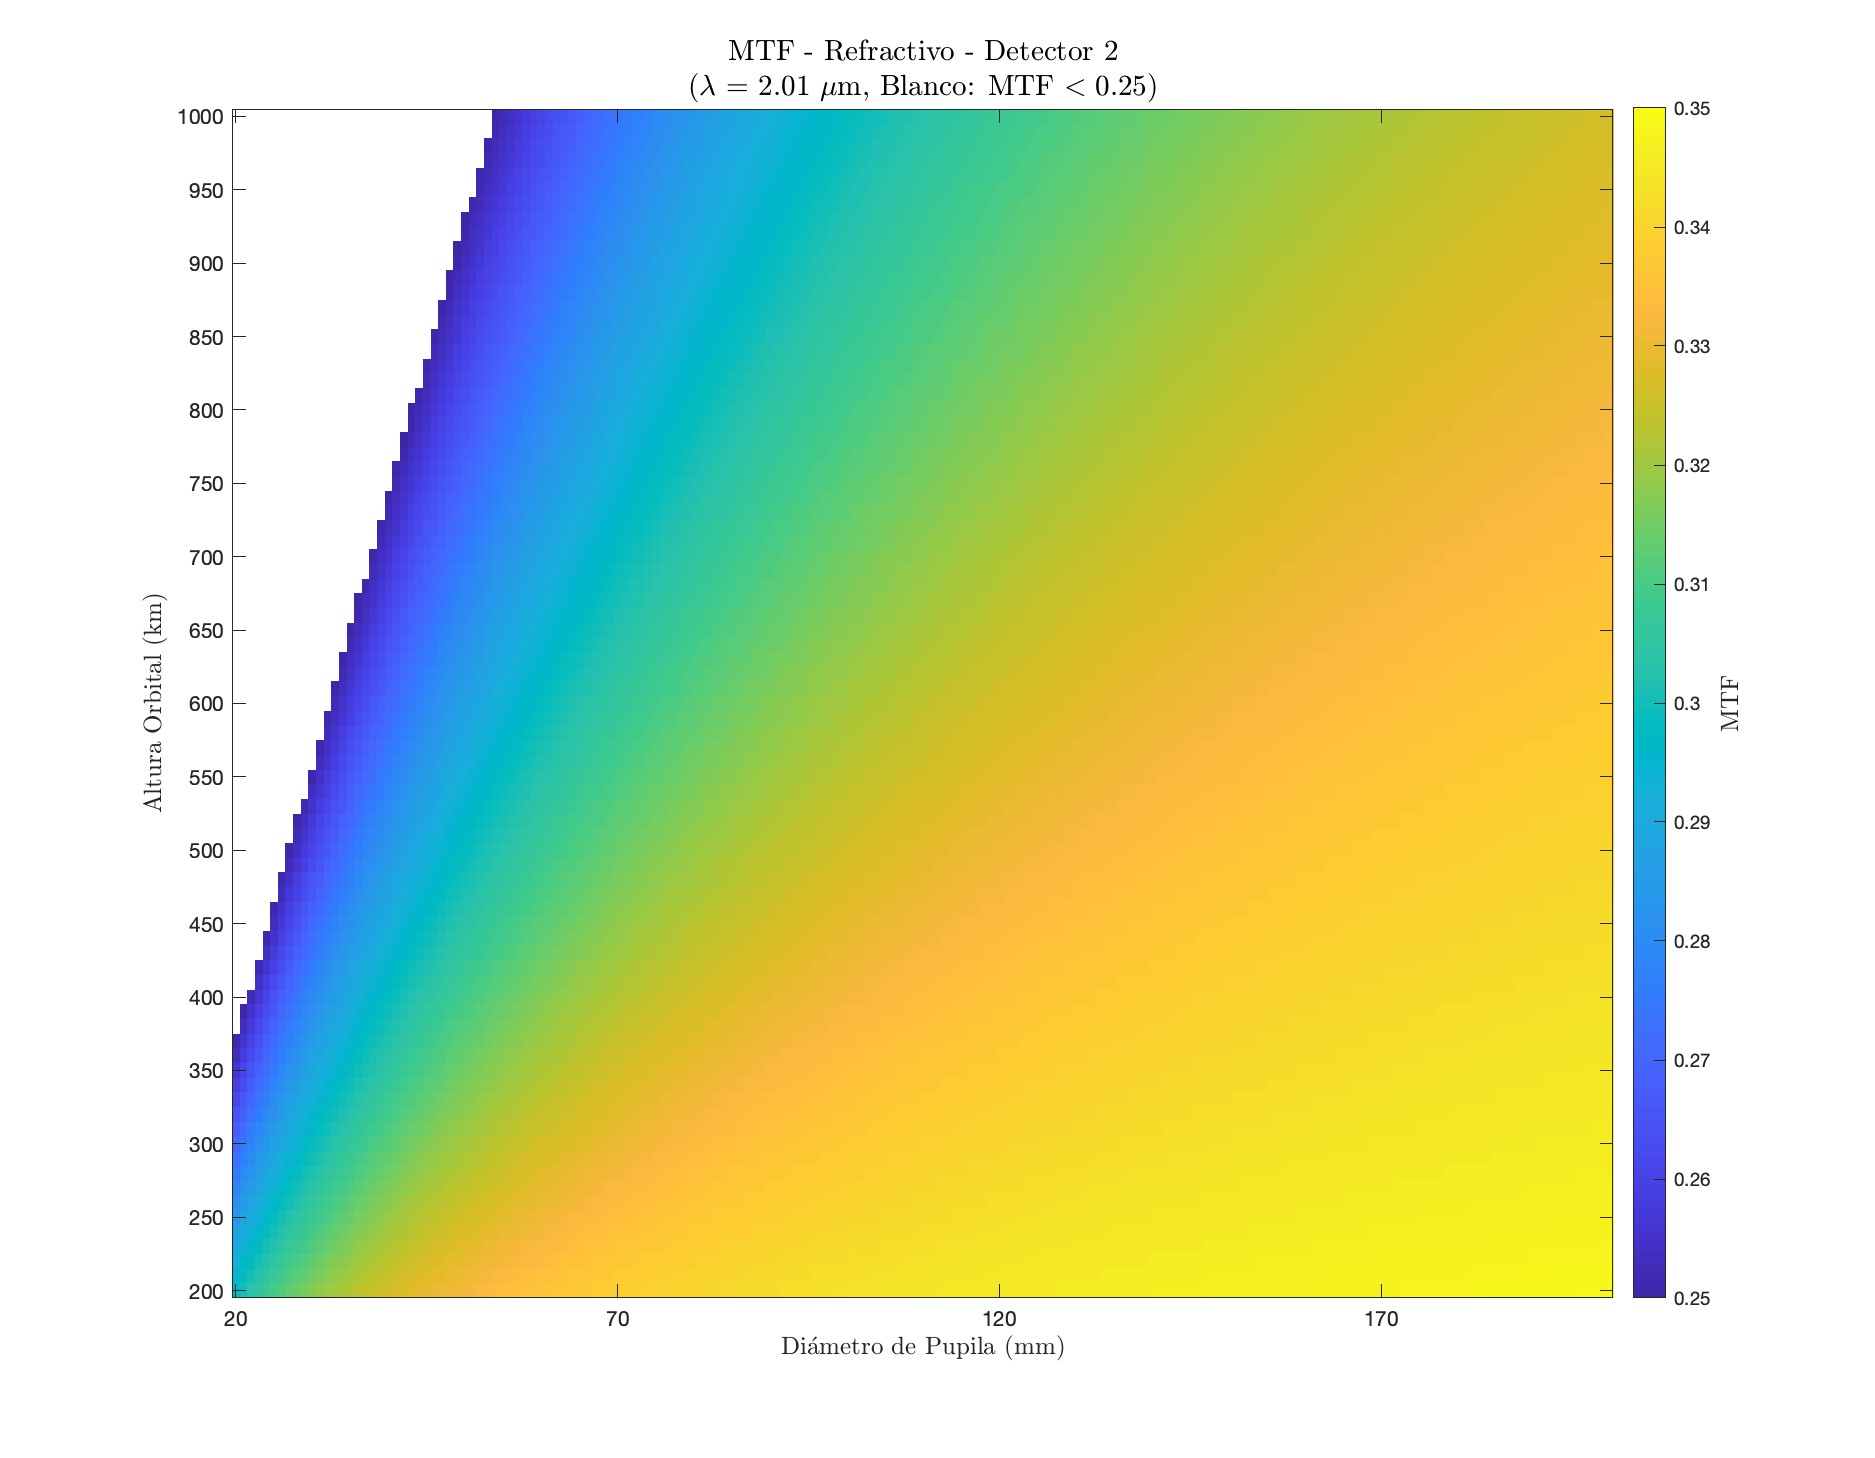
\includegraphics[width=0.48\linewidth]{4.Payload/MTF/MTF_Lambda2_Detector2_Telescopio1_heatmap.jpg} &
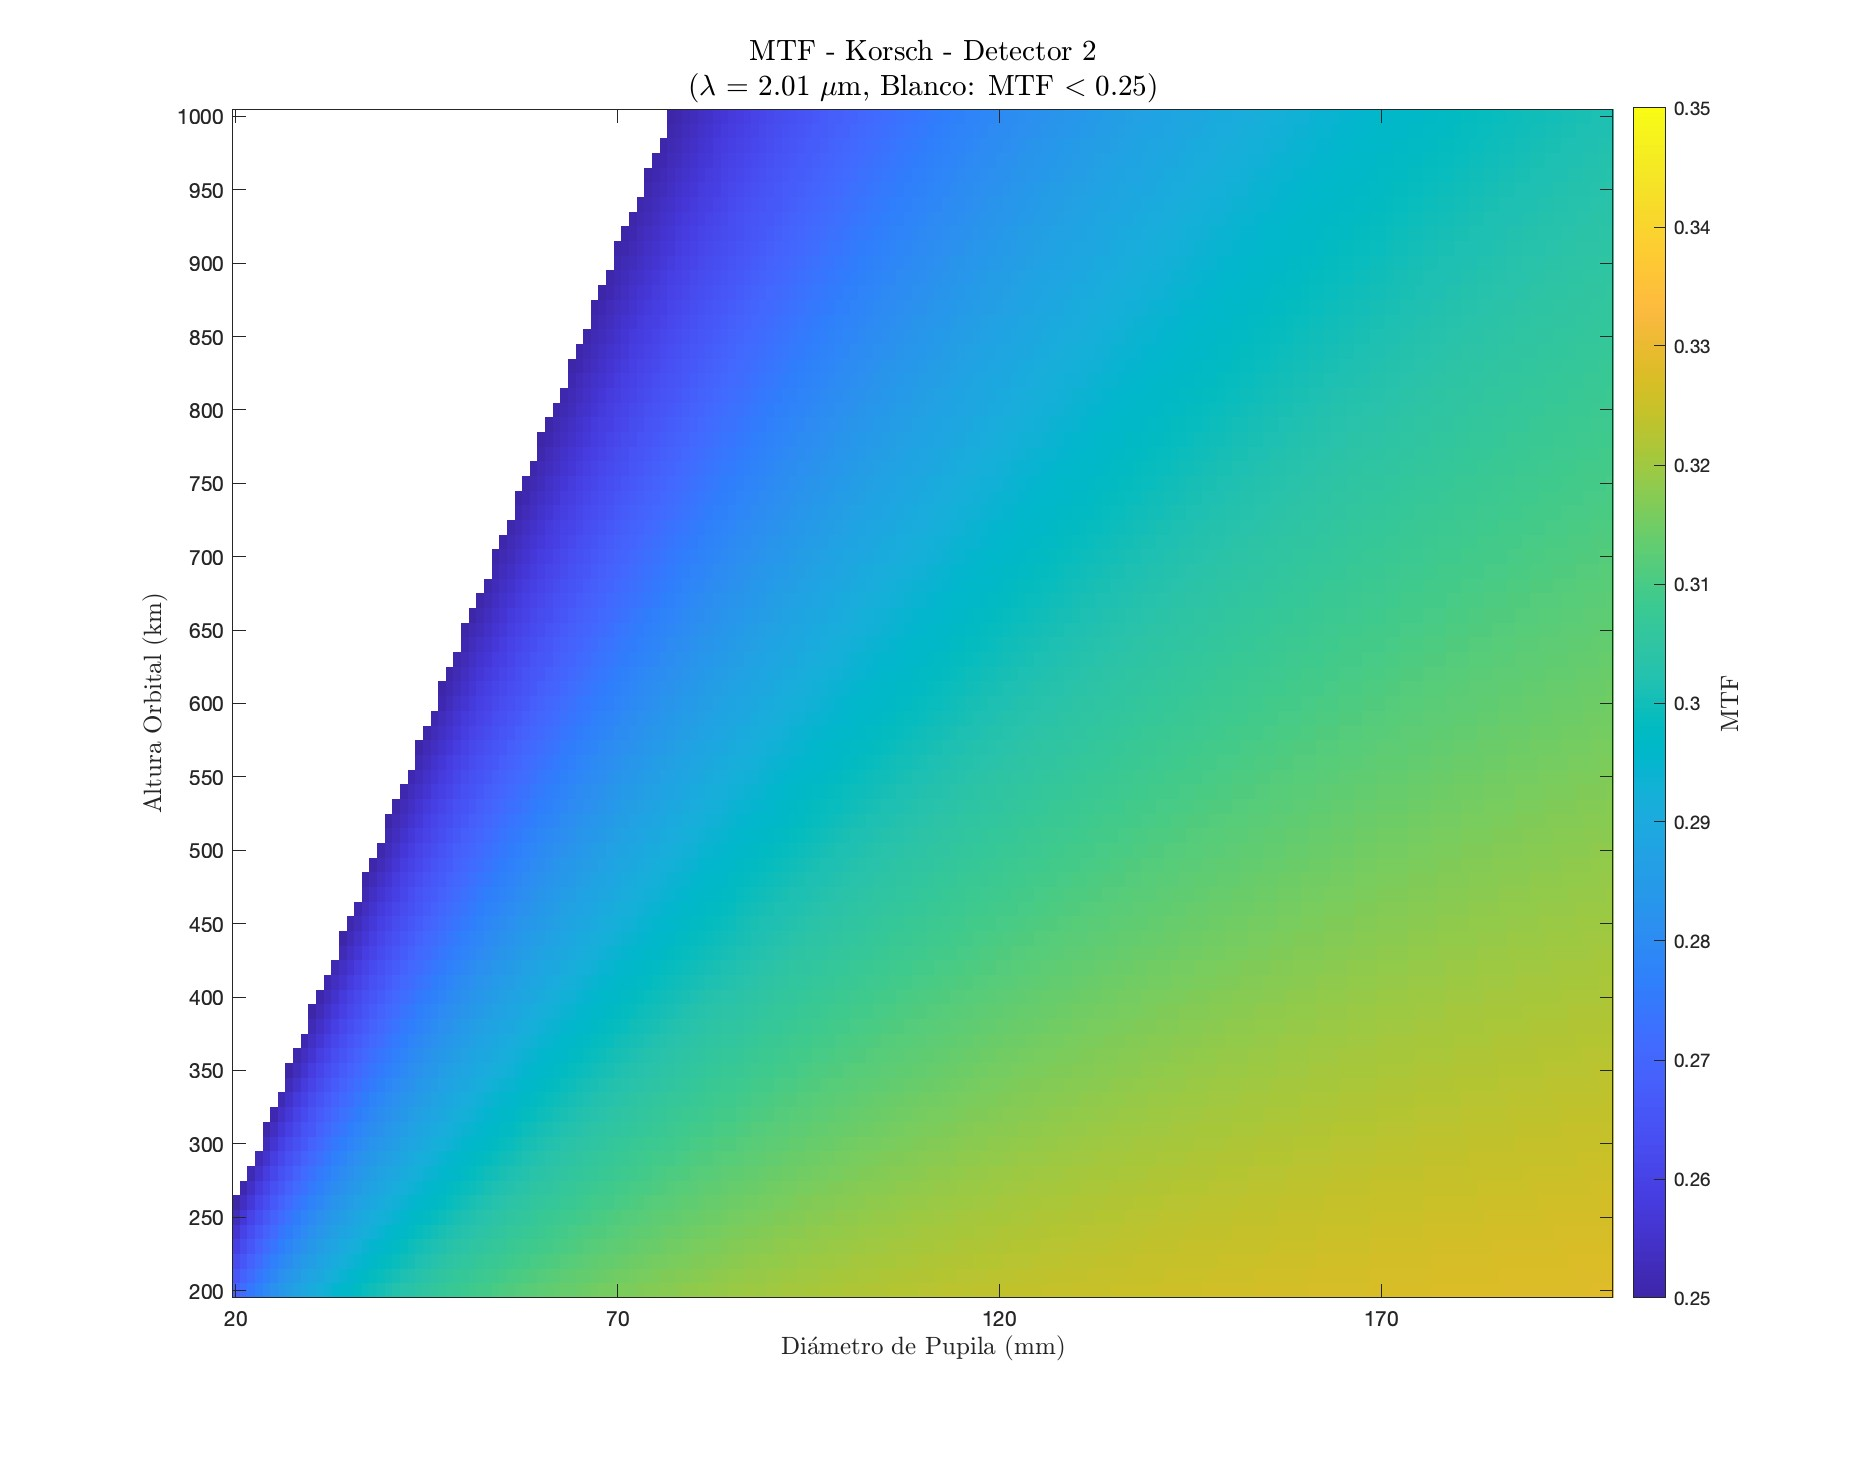
\includegraphics[width=0.48\linewidth]{4.Payload/MTF/MTF_Lambda2_Detector2_Telescopio2_heatmap.jpg} \\
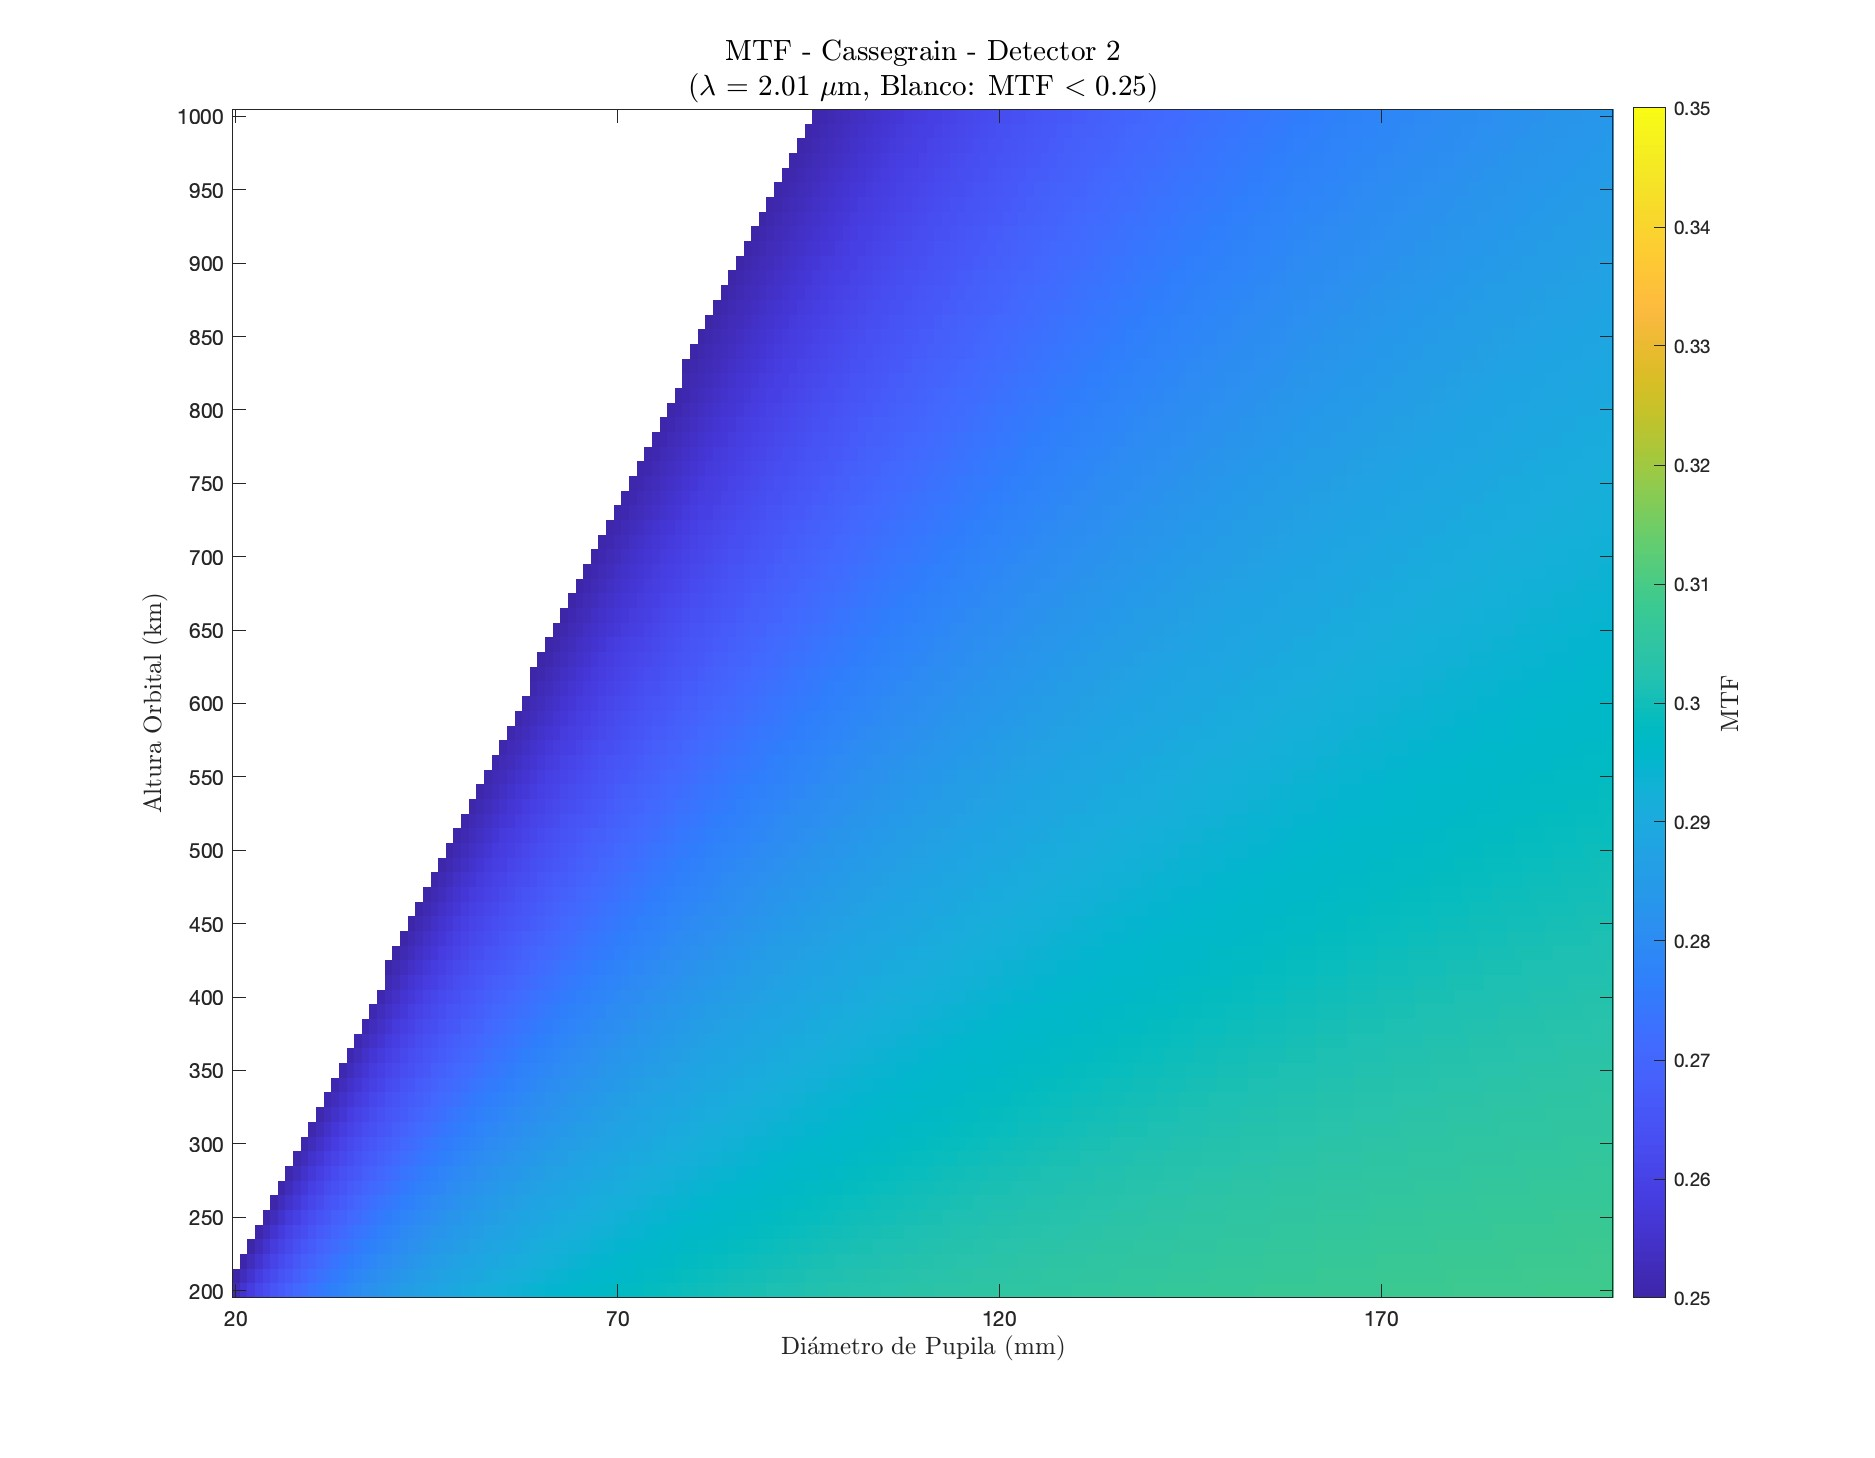
\includegraphics[width=0.48\linewidth]{4.Payload/MTF/MTF_Lambda2_Detector2_Telescopio3_heatmap.jpg} &
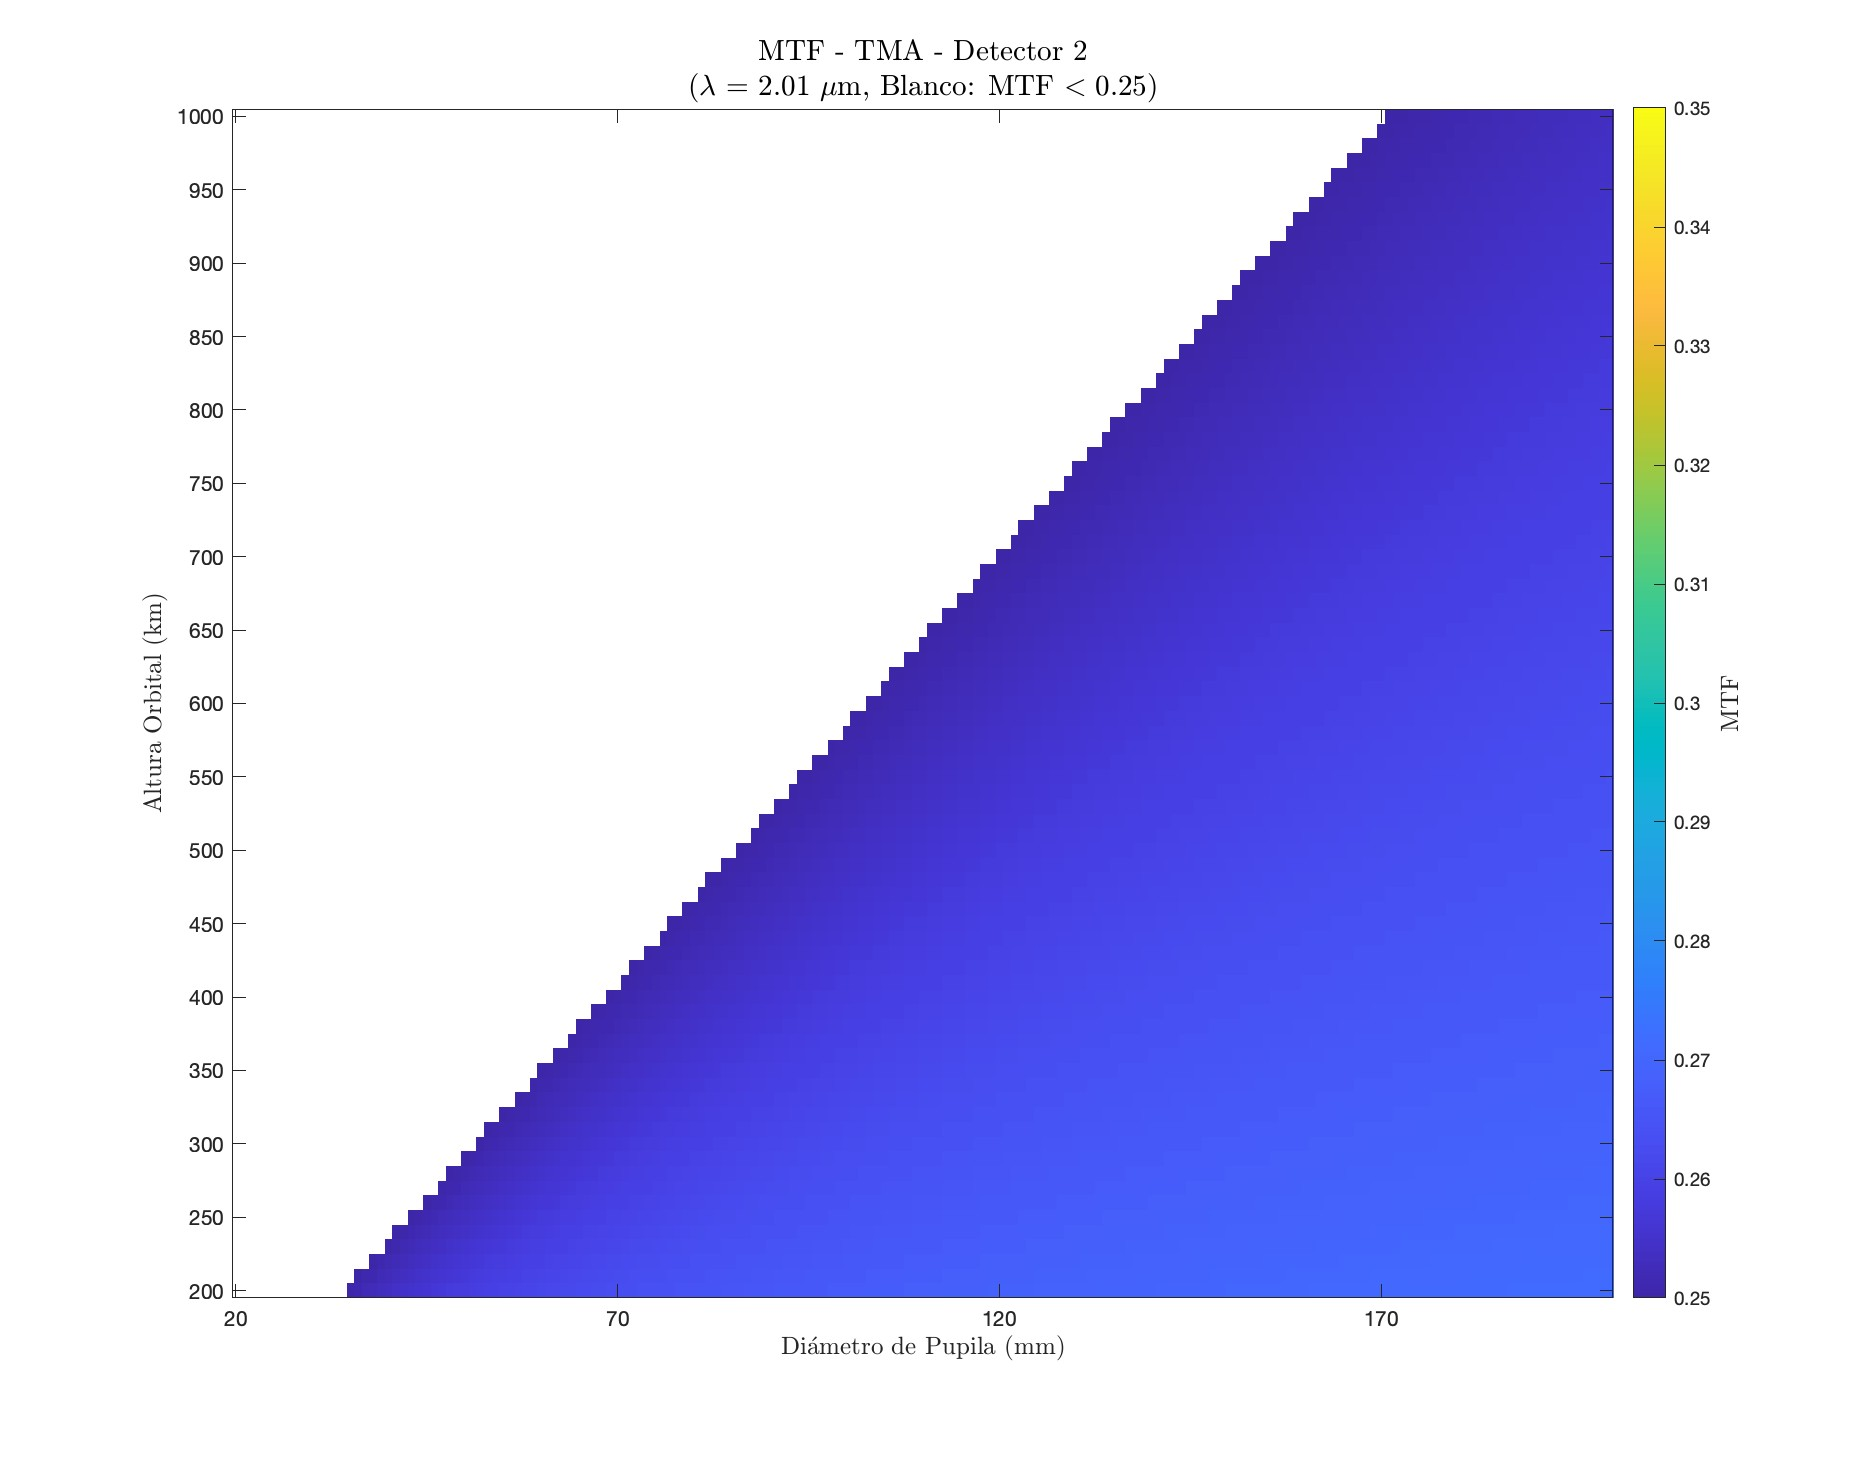
\includegraphics[width=0.48\linewidth]{4.Payload/MTF/MTF_Lambda2_Detector2_Telescopio4_heatmap.jpg} \\
\end{tabular}
\caption{Mapas de calor resultantes del calculo de MTF: Banda 2,01 \textmu m; Detector 2}
\end{figure}
\end{landscape}


%% DETECTOR 3
\begin{landscape}
\begin{figure}[p]
\centering
\setlength{\tabcolsep}{2pt}
\renewcommand{\arraystretch}{0}

\begin{tabular}{cc}
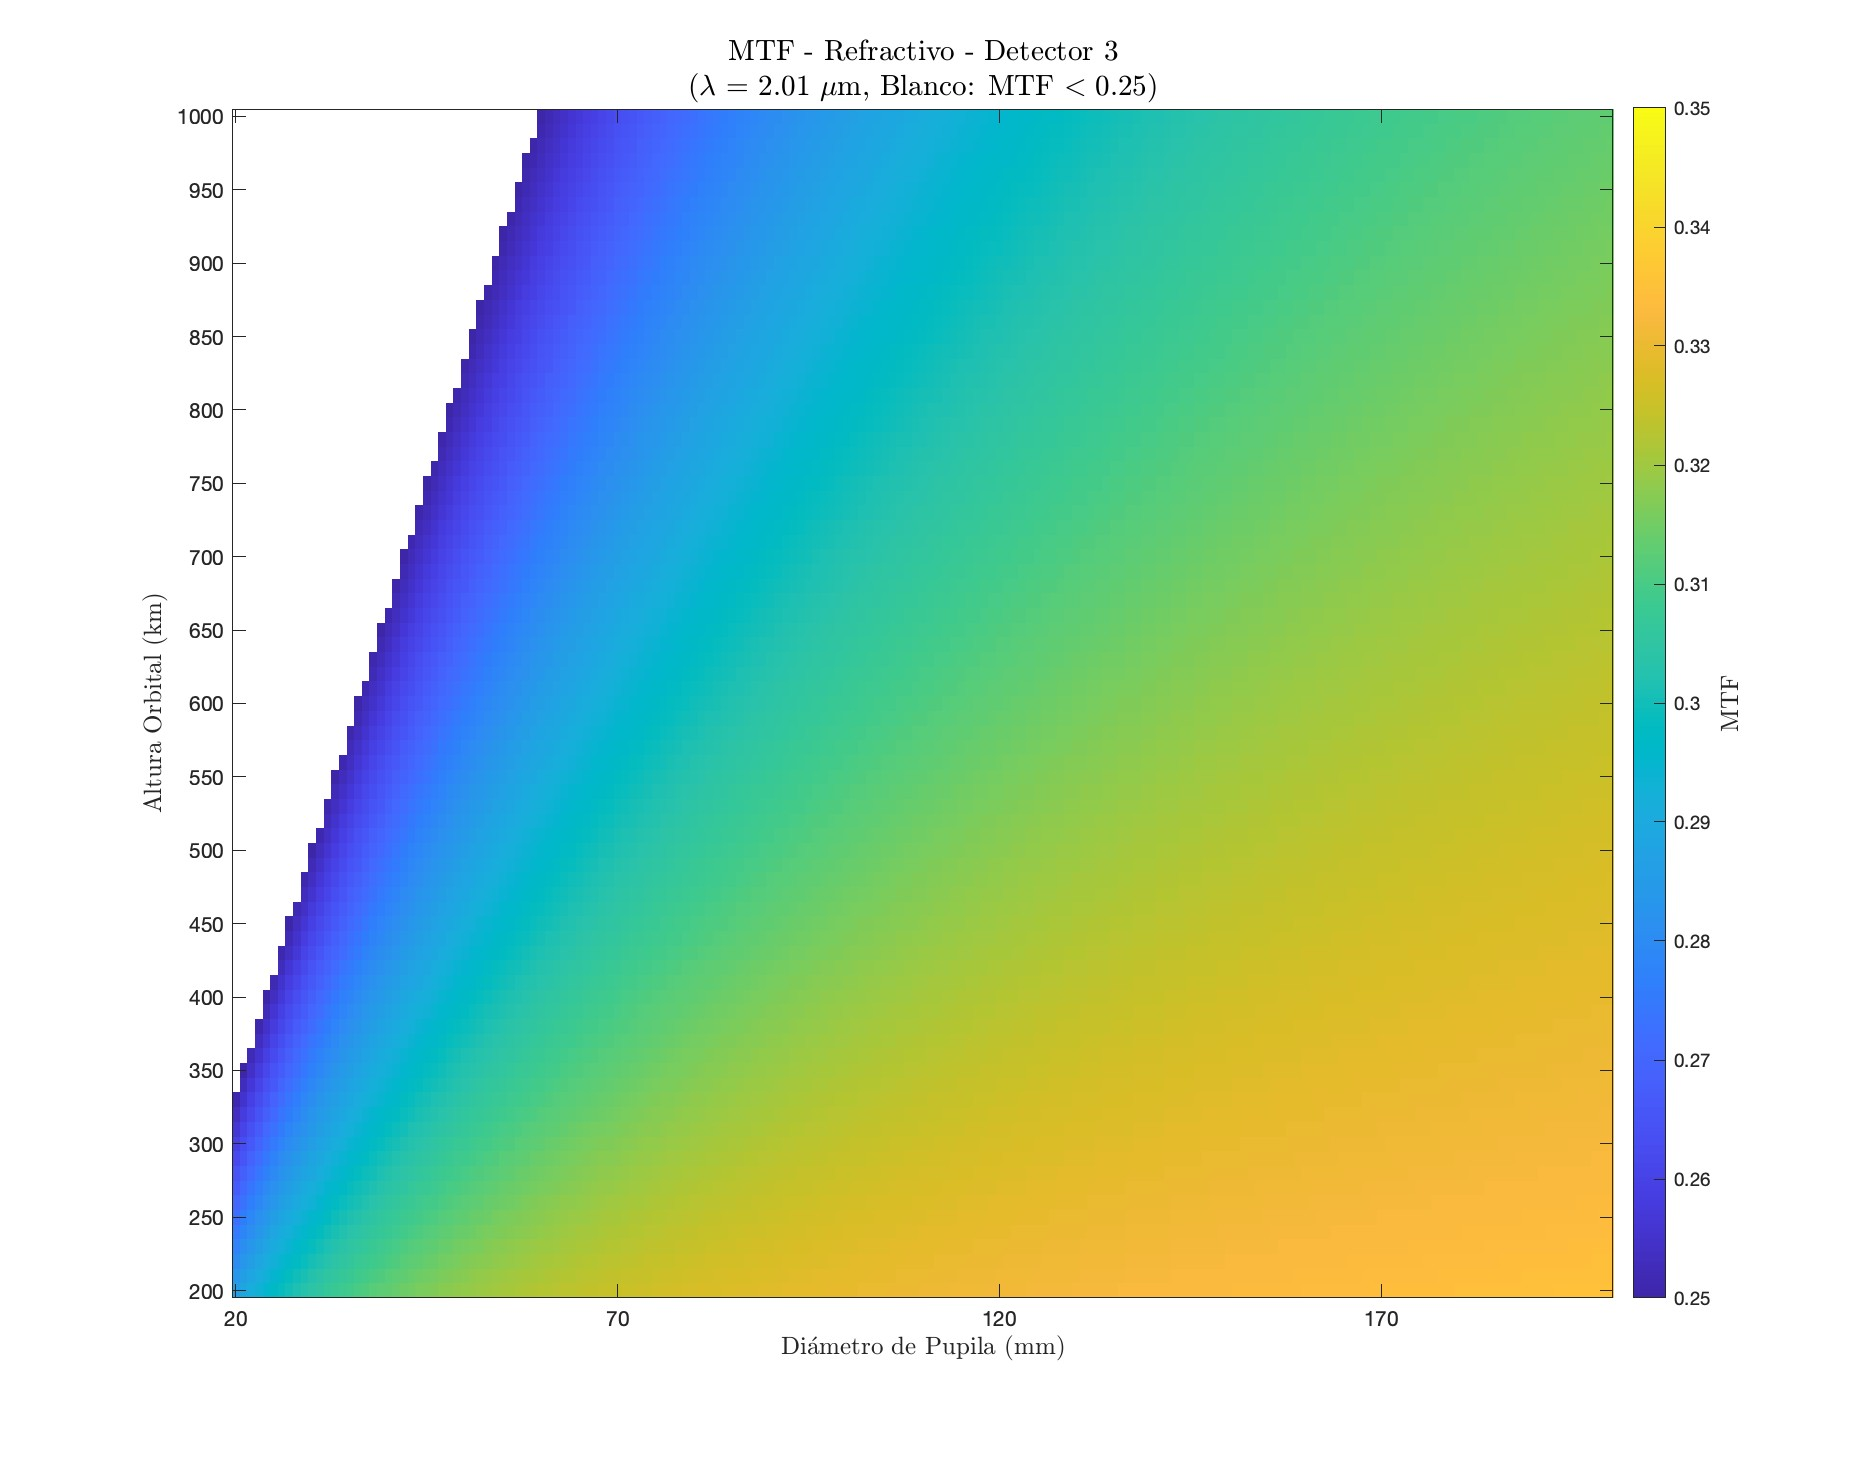
\includegraphics[width=0.48\linewidth]{4.Payload/MTF/MTF_Lambda2_Detector3_Telescopio1_heatmap.jpg} &
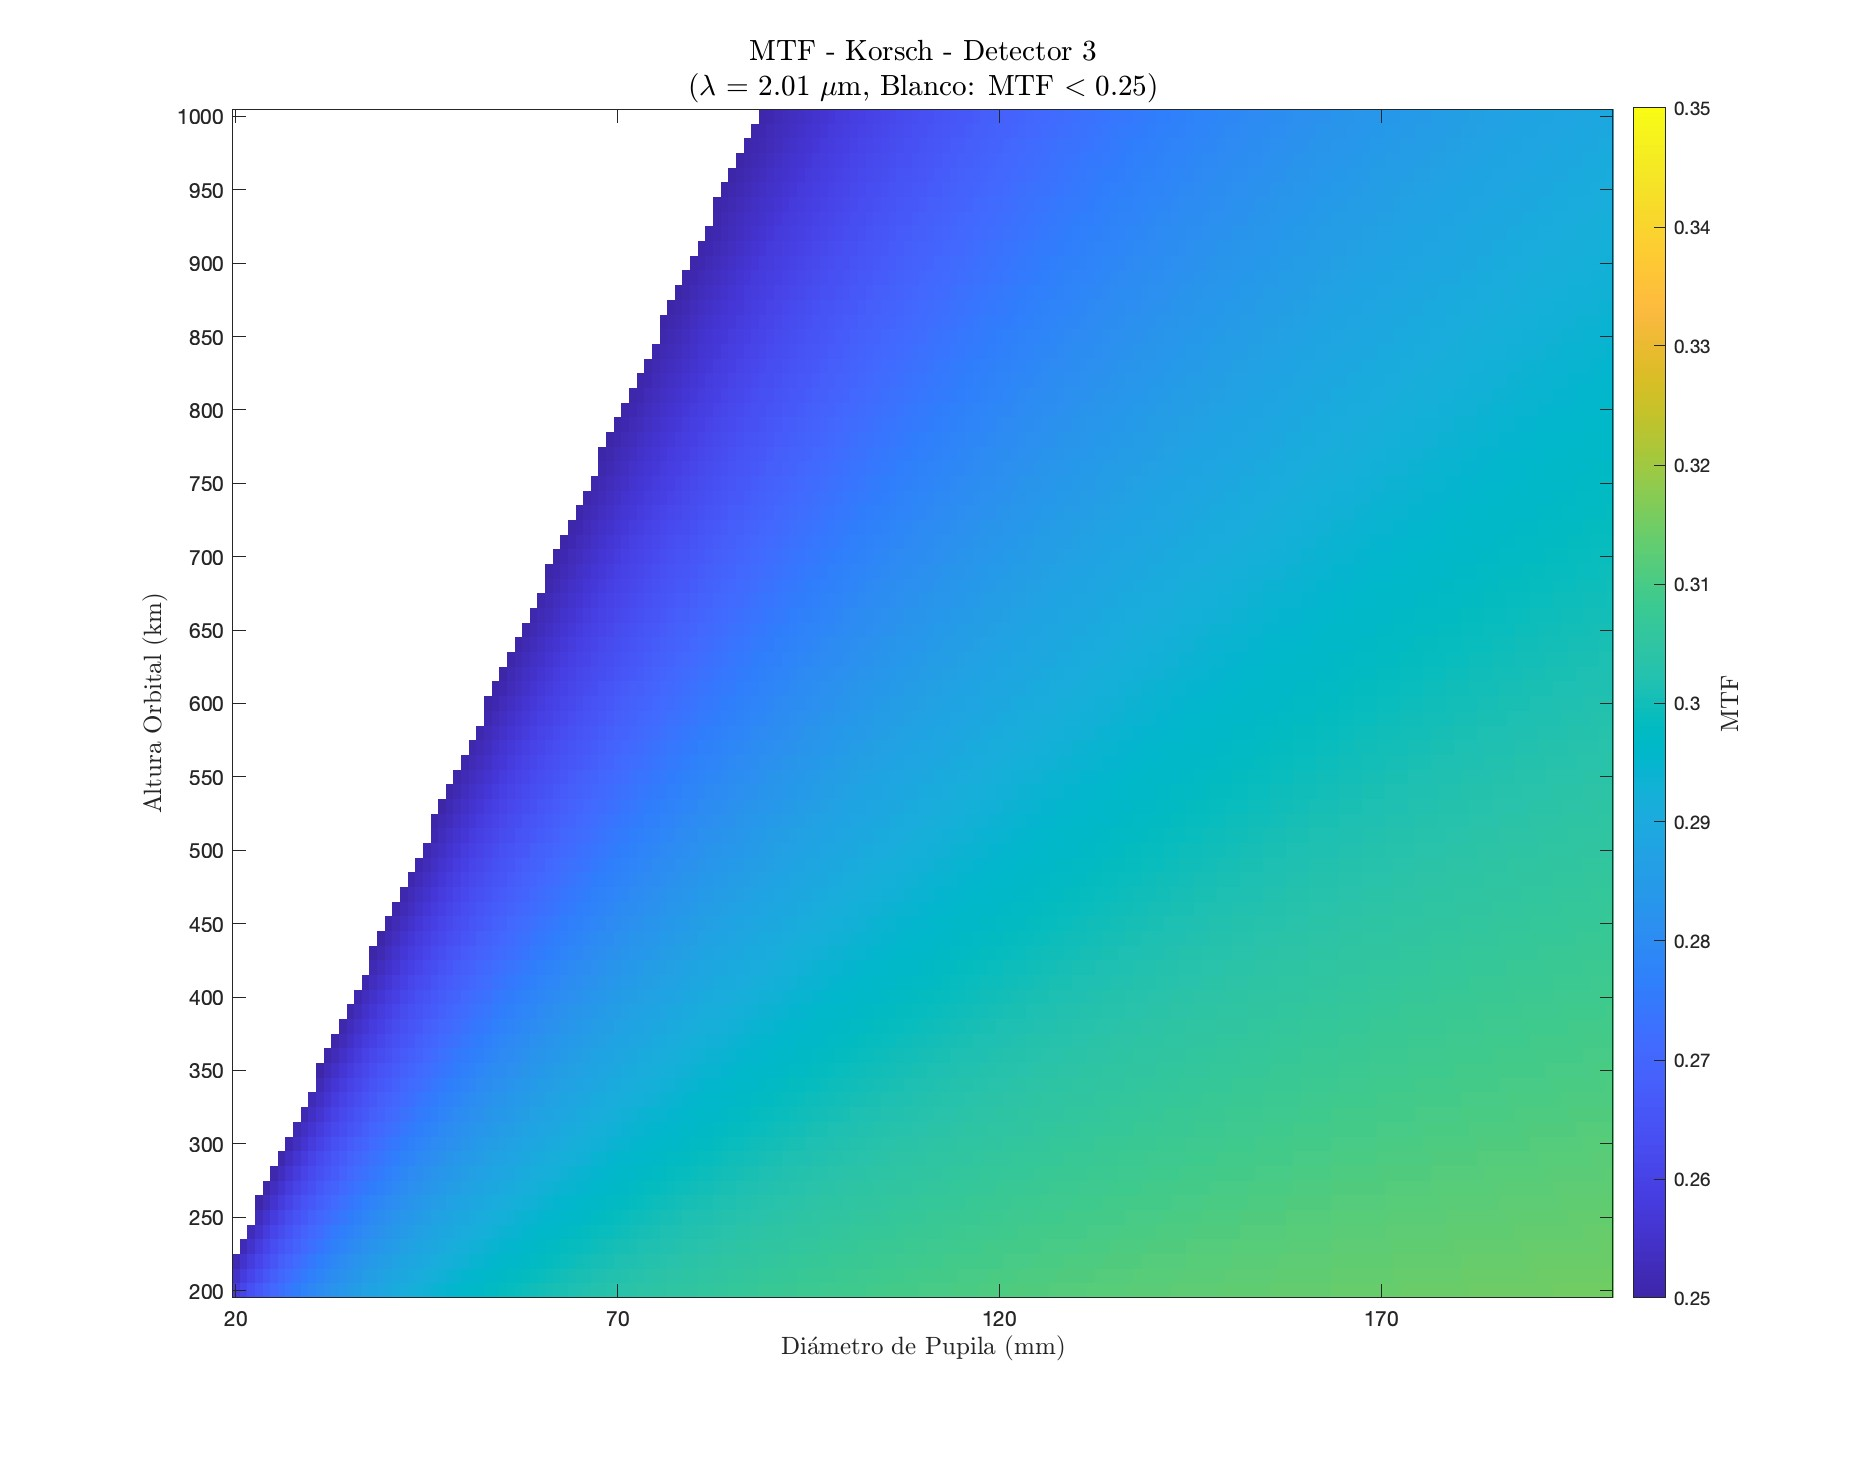
\includegraphics[width=0.48\linewidth]{4.Payload/MTF/MTF_Lambda2_Detector3_Telescopio2_heatmap.jpg} \\
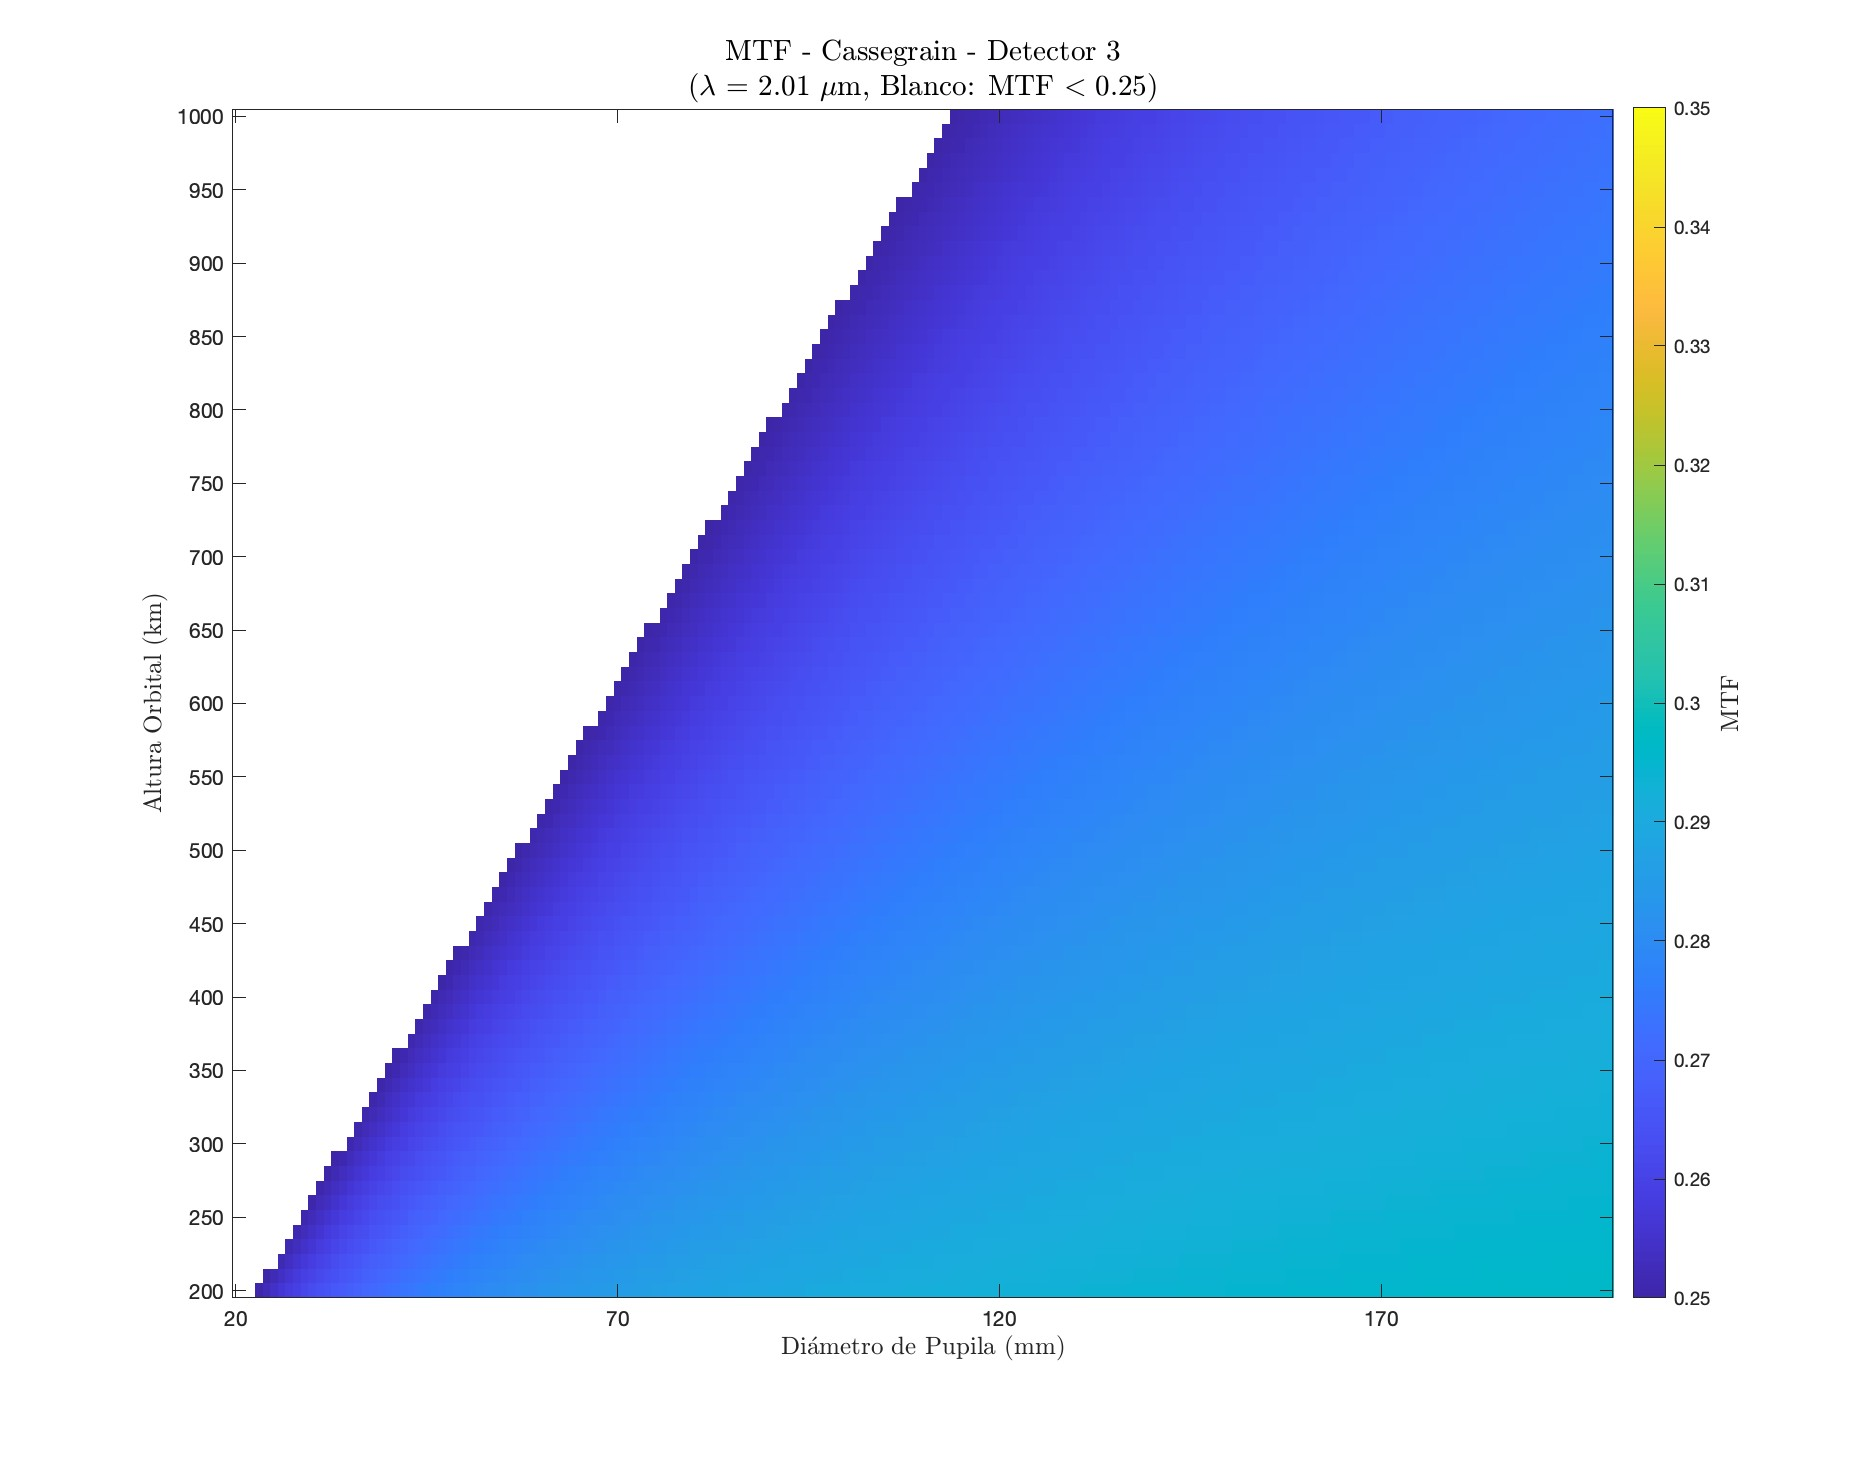
\includegraphics[width=0.48\linewidth]{4.Payload/MTF/MTF_Lambda2_Detector3_Telescopio3_heatmap.jpg} &
\includegraphics[width=0.48\linewidth]{4.Payload/MTF/MTF_Lambda2_Detector3_Telescopio4_heatmap.jpg} \\
\end{tabular}
\caption{Mapas de calor resultantes del calculo de MTF: Banda 2,01 \textmu m; Detector 3}
\end{figure}
\end{landscape}

Estos gráficos permiten extraer las siguientes consideraciones:

\begin{itemize}
    \item Como se aprecia, es un requisito que impone limitaciones considerables al diseño. No obstante, todavía aloja un espacio de diseño muy amplio, pues la única combinación no viable resulta en el detector 1 combinado con el telescopio TMA.
    \item El rendimiento más bajo, aunque con soluciones viables, es el detector 1, pues su MTF es la menor.
    \item De igual manera, es esperable, debido al alineamiento, que el telescopio con mejor rendimiento sea el refractivo, mientras el más pobre resulte el TMA.
\end{itemize}

\section{Cálculo de la SNR}

El cálculo de la relación señal-ruido (SNR) se ha realizado empleando las ecuaciones de la sección \ref{snr}. Para cada combinación de diámetro de pupila y altura orbital, y considerando los diferentes detectores y tipos de telescopio, se han generado mapas de calor que representan los valores de SNR obtenidos.

En este análisis se han utilizado los parámetro expuestos de detectores (tablas \ref{tab:detectores_comparacion_2}) y de telescopios(tabla \ref{tab:tabla_telescopios}), así como los parámetros iniciales especificados en la tabla \ref{initialsnr}, que incluyen tanto las características instrumentales como los valores de ruido en condiciones de peor caso. Este enfoque permite identificar, para cada configuración, las regiones del espacio de diseño que cumplen con los requisitos mínimos de SNR establecidos para la misión.


\begin{table}[H]
\centering
\caption{Parámetros iniciales y fuentes de ruido para el cálculo de SNR}
\begin{tabular}{l r}
\hline
\multicolumn{2}{c}{\textbf{Parámetros iniciales}} \\
\hline
TDI & 1\tablefootnote{un TDI=1 equivale a no implementado.} \\
Radiancia de referencia & 100 W/m\textsuperscript{2}·sr·\textmu m \\
\hline
\multicolumn{2}{c}{\textbf{Ruidos}\cite{gravrand_development_2017}} \\
\hline
$N_{dark}$ & 50 $e^-$  \\
$N_{read}$ & 100 $e^-$  \\
$N_{preamp}$ & 5 $e^-$  \\
$N_{video}$ & 10 $e^-$  \\
$N_{jitter}$ & 5 $e^-$  \\
$N_{emc}$ & 5 $e^-$  \\
$N_{quant}$ & 2 $e^-$  \\
$N_{nonlin}$ & 2 $e^-$  \\
\hline
\label{initialsnr}
\end{tabular}

\label{tab:parametros_ruidos}
\end{table}

De igual manera que en la computación del MTF total, se añade al \textbf{SNR un margen del 10\%} en calidad de reserva de diseño. En las etapas iniciales, los parámetros contribuyentes experimentan variaciones que pueden degradar el rendimiento del sistema. Este margen de seguridad permite absorber dichas desviaciones y garantizar el cumplimiento de los requisitos establecidos.

De nuevo, solo se presenta la banda más restrictiva. En este caso, será la de menor longitud de onda: la banda $0,76 \mu m$, ya que la longitud de onda es directamente proporcional a la irradiancia, y por ello, al número de electrones que recibe el detector. El resto se encuentran de nuevo en el anexo \ref{sec:annexdata}. A continuación se presentan las gráficas correspondientes, que muestran la variación de la SNR en función del diámetro de pupila y la altura orbital para las distintas opciones de detectores y telescopios evaluados:

%% GRAFICAS SNR

%% Lambda 3

\begin{landscape}
\begin{figure}[p]
\centering
\vspace*{0.3cm}


\vspace{0.3cm}
\setlength{\tabcolsep}{4pt}
\renewcommand{\arraystretch}{0}

\begin{tabular}{cc}
\includegraphics[width=0.48\linewidth]{4.Payload/SNR/SNR_Lambda3_Detector4_Telescopio1_heatmap.jpg} &
\includegraphics[width=0.48\linewidth]{4.Payload/SNR/SNR_Lambda3_Detector4_Telescopio2_heatmap.jpg} \\
\includegraphics[width=0.48\linewidth]{4.Payload/SNR/SNR_Lambda3_Detector4_Telescopio3_heatmap.jpg} &
\includegraphics[width=0.48\linewidth]{4.Payload/SNR/SNR_Lambda3_Detector4_Telescopio4_heatmap.jpg} \\
\end{tabular}
\caption{Mapas de calor resultantes del calculo de SNR: Banda 0,76 \textmu m; Detector 1}
\end{figure}
\end{landscape}

% Detector 2
\begin{landscape}
\begin{figure}[p]
\centering
\vspace*{0.3cm}

\vspace{0.3cm}
\setlength{\tabcolsep}{4pt}
\renewcommand{\arraystretch}{0}

\begin{tabular}{cc}
\includegraphics[width=0.48\linewidth]{4.Payload/SNR/SNR_Lambda3_Detector5_Telescopio1_heatmap.jpg} &
\includegraphics[width=0.48\linewidth]{4.Payload/SNR/SNR_Lambda3_Detector5_Telescopio2_heatmap.jpg} \\
\includegraphics[width=0.48\linewidth]{4.Payload/SNR/SNR_Lambda3_Detector5_Telescopio3_heatmap.jpg} &
\includegraphics[width=0.48\linewidth]{4.Payload/SNR/SNR_Lambda3_Detector5_Telescopio4_heatmap.jpg} \\
\end{tabular}
\caption{Mapas de calor resultantes del calculo de SNR: Banda 0,76 \textmu m; Detector 2}
\end{figure}
\end{landscape}

% Detector 3
\begin{landscape}
\begin{figure}[p]
\centering
\vspace*{0.3cm}

\vspace{0.3cm}
\setlength{\tabcolsep}{4pt}
\renewcommand{\arraystretch}{0}

\begin{tabular}{cc}
\includegraphics[width=0.48\linewidth]{4.Payload/SNR/SNR_Lambda3_Detector6_Telescopio1_heatmap.jpg} &
\includegraphics[width=0.48\linewidth]{4.Payload/SNR/SNR_Lambda3_Detector6_Telescopio2_heatmap.jpg} \\
\includegraphics[width=0.48\linewidth]{4.Payload/SNR/SNR_Lambda3_Detector6_Telescopio3_heatmap.jpg} &
\includegraphics[width=0.48\linewidth]{4.Payload/SNR/SNR_Lambda3_Detector6_Telescopio4_heatmap.jpg} \\
\end{tabular}
\caption{Mapas de calor resultantes del calculo de SNR: Banda 0,76 \textmu m; Detector 3}
\end{figure}
\end{landscape}


De la interpretación de estos gráficos se obtienen las siguientes apreciaciones:

\begin{itemize}
    \item Este es, con diferencia, el requisito de misión menos restrictivo para el trabajo, pues, con los grandes tamaños de pixel y buenas eficiencias cuánticas del detector, junto con longitudes de onda mayores al visible, es sencillo conseguir altos valores de SNR.
    \item Se puede descartar la incorporación de TDI, ya que con una integración simple se captura una relación señal ruido que cumple holgadamente con el requisito de la misión para todos los casos. 
\end{itemize}

\section{Cobertura de la región de interés: Swath, FoV y tiempo de revisita}

Otro de los requerimientos impuestos por el cliente es el obtener un mapa cada 7 días en la región, o lo que es lo mismo, un tiempo de revisita de 7 días o menor. Si se comparan con otras misiones de observación similares, se puede observar que es un tiempo exigente que requiere habitualmente de una constelación por lo que será de los parámetros más limitantes a la hora de encontrar la solución óptima:

%% Ejemplos cobertura
\begin{table}[H]
\caption{Comparativa de tiempos de revisita de misiones satelitales.}
\centering
\begin{tabular}{@{}llll@{}}
\toprule
             & Nº Satélites & \textit{Swath} (km) & Tiempo revisita\tablefootnote{Estos valores son más favorables que los calculados en este trabajo, pues no se consideran los factores limitantes descritos en esta página. Por ello, no serán directamente comparables a los resultados obtenidos, aunque permite hacerse una idea aproximada de la solución} (días) \\ \midrule
Landsat 8 \cite{li2020global}   & 1                & 185                 & 16                     \\
Landsat Next \cite{copernicus2025sentinel} & 3                & 164                 & 6                      \\
Sentinel-2  \cite{neigh2023landsat} & 2                & 290                 & 5                      \\ \bottomrule
\end{tabular}

\label{tab:revisitlandsat}
\end{table}


Además, se tendrán en cuenta 2 factores adicionales para el cálculo:
\begin{itemize}
    \item \textbf{Solapamiento del swath}: Para asegurar la cobertura completa de la región entre pasadas, se establece un \textbf{factor de solapamiento del swath mínimo del 5\%} que compensa posibles desviaciones en la proyección del swath y pérdidas de altura del satélite antes de la reinyección orbital.
    \item \textbf{Cobertura de nubes}: A diferencia de otros sistemas de observación, como el SAR (Radar de Apertura Sintética, o \textit{Synthetic Aperture Radar}, \cite{lou2020sar}), los detectores SWIR pasivos no son capaces de capturar la señal de la superficie terrestre a través de los cúmulos nubosos. Según el enunciado impuesto, \say{\textit{la cobertura de nubes sobre EE. UU. es un día cubierto por cada cinco descubiertos}}, por lo que se considera un \textbf{factor de 1/6 de pasadas del satélite no efectivas}.
\end{itemize}

\begin{figure}[H]
    \centering
    \begin{subfigure}[t]{0.45\textwidth}
        \centering
        \includegraphics[width=\linewidth]{4.Payload/TFG_Tikz-1.jpg}
        \caption{Solapamiento del swath. \\ Fuente: Elaboración propia}
        \label{fig:img3}
    \end{subfigure}
    \hspace{0.05\textwidth}
    \begin{subfigure}[t]{0.45\textwidth}
        \centering
        \includegraphics[width=\linewidth]{4.Payload/cloudcov.png}
        \caption{Datos no válidos debido a cobertura de nubes de la misión Landsat, en rojo. \\ Fuente: \cite{osullivan2023removing}}
        \label{fig:img4}
    \end{subfigure}
    \caption{Factores de limitación del swath en el problema de la cobertura}
\end{figure}


Para realizar la computación de la cobertura en la región de interés, se va a utilizar un software \textit{open-source} desarrollado en el paper \textit{A Semi-Analytical Method for Calculating Revisit Time for Satellite Constellations with Discontinuous Coverage} \cite{crisp2018semi}. Para aplicar dicho código al presente trabajo, se ha desarrollado un \textit{wrapper}, es decir, una función que actúa como interfaz de adaptación entre los parámetros específicos del presente estudio y las funciones originales del software mencionado. Con ello, se pueden extraer mapas de calor que expongan, en función de la altura orbital y el \textit{swath}\footnote{Discretizados ambos en pasos de 10 km}, los tiempos de revisita necesarios para la región de interés. Evaluaremos distintas configuraciones:

\begin{itemize}
    \item Configuración (i): 1 único satélite con 1 telescopio embarcado.
    \item Config. (ii): 1 satélite con 2 telescopios embarcados. Los telescopios serán dispuestos según la Figura \ref{fig:img1}, esencialmente duplicando el FoV límite.
    \item Config. (iii): Constelación de 2 satélites ($i:2/1/0$\footnote{Escrito en notación de Walker \cite{walker1991phase}}).
    \item Config. (iv): Constelación de 2 satélites, con 2 telescopios embarcados en cada uno. ($i:2/1/0$).
    \item Config. (v): Constelación de 3 satélites ($i:3/1/0$).
\end{itemize}

En todas las constelaciones, los satélites se dispondrán desfasados en anomalía verdadera de manera que $\Delta \nu = 360º/n $ siendo $n =$ Nº satélites, dentro de la misma órbita (véase Figura \ref{fig:img2}). Esto permite reducir en un factor de $n$ la distancia entre pasadas a medida que rota la Tierra, consiguiendo tiempos de revisita menores, manteniendo así para todos los satélites el mismo valor de LTAN.

\begin{figure}[H]
    \centering
    \begin{subfigure}[t]{0.45\textwidth}
        \centering
        \includegraphics[width=\linewidth]{4.Payload/TFG_Tikz-2.jpg}
        \caption{Disposición de dos telescopios embarcados en un satélite. \\ Fuente: Elaboración propia}
        \label{fig:img1}
    \end{subfigure}
    \hspace{0.05\textwidth}
    \begin{subfigure}[t]{0.45\textwidth}
        \centering
        \includegraphics[width=\linewidth]{4.Payload/TFG_Tikz-3.jpg}
        \caption{Desfase de la constelación de satélites en anomalía verdadera. \\ Fuente: Elaboración propia.}
        \label{fig:img2}
    \end{subfigure}
    \caption{Esquemas de las configuraciones evaluadas en el problema de la cobertura.}
    \label{fig:configs}
\end{figure}

Se consideran dos limitaciones al \textit{swath}:
\begin{itemize}
    \item El FoV de cada telescopio, definido en la tabla \ref{tab:tabla_telescopios}, que limita el swath en función de la altura, mediante la relación \ref{fov}
    \item El array del detector, mediante la ecuación \ref{swath}. Para ampliarlo y dar más flexibilidad a esta restricción, se considera el uso de hasta 3 detectores en linea.
\end{itemize}

Además, solo se considerará el territorio EE. UU. continental, con una \textbf{latitud inferior límite de 25º N}. Ya que el interés del cliente reside en el mapeo de las principales ciudades, se pueden excluir, por simplicidad de cálculo, otros territorios del país como Hawaii, Puerto Rico y otros territorios de ultramar. Con ello, se procede a realizar la computación y exponer los resultados en las siguientes páginas:

%% Graficas 2 SAT 2TEL
\begin{landscape}
\begin{figure}[p]
\centering
\vspace*{0.3cm}
\setlength{\tabcolsep}{4pt}
\renewcommand{\arraystretch}{0}
\begin{tabular}{cc}
\includegraphics[width=0.48\linewidth]{4.Payload/Coverage/heatmap_2 Satelite(s); 2 Telescopio(s): Refractivo; Detector 1.jpg} &
\includegraphics[width=0.48\linewidth]{4.Payload/Coverage/heatmap_2 Satelite(s); 2 Telescopio(s): Korsch; Detector 1.jpg} \\
\includegraphics[width=0.48\linewidth]{4.Payload/Coverage/heatmap_2 Satelite(s); 2 Telescopio(s): Cassegrain; Detector 1.jpg} &
\includegraphics[width=0.48\linewidth]{4.Payload/Coverage/heatmap_2 Satelite(s); 2 Telescopio(s): TMA; Detector 1.jpg} \\
\end{tabular}
\caption{Mapas de calor resultantes del cálculo de cobertura para el Detector 1, con 2 satélites y 2 telescopios.}
\end{figure}
\end{landscape}

\begin{landscape}
\begin{figure}[p]
\centering
\vspace*{0.3cm}
\setlength{\tabcolsep}{4pt}
\renewcommand{\arraystretch}{0}
\begin{tabular}{cc}
\includegraphics[width=0.48\linewidth]{4.Payload/Coverage/heatmap_2 Satelite(s); 2 Telescopio(s): Refractivo; Detector 2.jpg} &
\includegraphics[width=0.48\linewidth]{4.Payload/Coverage/heatmap_2 Satelite(s); 2 Telescopio(s): Korsch; Detector 2.jpg} \\
\includegraphics[width=0.48\linewidth]{4.Payload/Coverage/heatmap_2 Satelite(s); 2 Telescopio(s): Cassegrain; Detector 2.jpg} &
\includegraphics[width=0.48\linewidth]{4.Payload/Coverage/heatmap_2 Satelite(s); 2 Telescopio(s): TMA; Detector 2.jpg} \\
\end{tabular}
\caption{Mapas de calor resultantes del cálculo de cobertura para el Detector 2, con 2 satélites y 2 telescopios.}
\end{figure}
\end{landscape}

\begin{landscape}
\begin{figure}[p]
\centering
\vspace*{0.3cm}
\setlength{\tabcolsep}{4pt}
\renewcommand{\arraystretch}{0}
\begin{tabular}{cc}
\includegraphics[width=0.48\linewidth]{4.Payload/Coverage/heatmap_2 Satelite(s); 2 Telescopio(s): Refractivo; Detector 3.jpg} &
\includegraphics[width=0.48\linewidth]{4.Payload/Coverage/heatmap_2 Satelite(s); 2 Telescopio(s): Korsch; Detector 3.jpg} \\
\includegraphics[width=0.48\linewidth]{4.Payload/Coverage/heatmap_3 Satelite(s); 1 Telescopio(s): Cassegrain; Detector 3.jpg} &
\includegraphics[width=0.48\linewidth]{4.Payload/Coverage/heatmap_2 Satelite(s); 2 Telescopio(s): TMA; Detector 3.jpg} \\
\end{tabular}
\caption{Mapas de calor resultantes del cálculo de cobertura para el Detector 3, con 2 satélites y 2 telescopios.}
\end{figure}
\end{landscape}


%% Graficas 3 SAT
\begin{landscape}
\begin{figure}[p]
\centering
\vspace*{0.3cm}
\setlength{\tabcolsep}{4pt}
\renewcommand{\arraystretch}{0}
\begin{tabular}{cc}
\includegraphics[width=0.48\linewidth]{4.Payload/Coverage/heatmap_3 Satelite(s); 1 Telescopio(s): Refractivo; Detector 1.jpg} &
\includegraphics[width=0.48\linewidth]{4.Payload/Coverage/heatmap_3 Satelite(s); 1 Telescopio(s): Korsch; Detector 1.jpg} \\
\includegraphics[width=0.48\linewidth]{4.Payload/Coverage/heatmap_3 Satelite(s); 1 Telescopio(s): Cassegrain; Detector 1.jpg} &
\includegraphics[width=0.48\linewidth]{4.Payload/Coverage/heatmap_3 Satelite(s); 1 Telescopio(s): TMA; Detector 1.jpg} \\
\end{tabular}
\caption{Mapas de calor resultantes del cálculo de cobertura para el Detector 1, con 3 satélites.}
\end{figure}
\end{landscape}

\begin{landscape}
\begin{figure}[p]
\centering
\vspace*{0.3cm}
\setlength{\tabcolsep}{4pt}
\renewcommand{\arraystretch}{0}
\begin{tabular}{cc}
\includegraphics[width=0.48\linewidth]{4.Payload/Coverage/heatmap_3 Satelite(s); 1 Telescopio(s): Refractivo; Detector 2.jpg} &
\includegraphics[width=0.48\linewidth]{4.Payload/Coverage/heatmap_3 Satelite(s); 1 Telescopio(s): Korsch; Detector 2.jpg} \\
\includegraphics[width=0.48\linewidth]{4.Payload/Coverage/heatmap_3 Satelite(s); 1 Telescopio(s): Cassegrain; Detector 2.jpg} &
\includegraphics[width=0.48\linewidth]{4.Payload/Coverage/heatmap_3 Satelite(s); 1 Telescopio(s): TMA; Detector 2.jpg} \\
\end{tabular}
\caption{Mapas de calor resultantes del cálculo de cobertura para el Detector 2, con 3 satélites.}
\end{figure}
\end{landscape}

\begin{landscape}
\begin{figure}[p]
\centering
\vspace*{0.3cm}
\setlength{\tabcolsep}{4pt}
\renewcommand{\arraystretch}{0}
\begin{tabular}{cc}
\includegraphics[width=0.48\linewidth]{4.Payload/Coverage/heatmap_3 Satelite(s); 1 Telescopio(s): Refractivo; Detector 3.jpg} &
\includegraphics[width=0.48\linewidth]{4.Payload/Coverage/heatmap_3 Satelite(s); 1 Telescopio(s): Korsch; Detector 3.jpg} \\
\includegraphics[width=0.48\linewidth]{4.Payload/Coverage/heatmap_3 Satelite(s); 1 Telescopio(s): Cassegrain; Detector 3.jpg} &
\includegraphics[width=0.48\linewidth]{4.Payload/Coverage/heatmap_3 Satelite(s); 1 Telescopio(s): TMA; Detector 3.jpg} \\
\end{tabular}
\caption{Mapas de calor resultantes del cálculo de cobertura para el Detector 3, con 3 satélites.}
\end{figure}
\end{landscape}


De ello, se pueden extraer las siguientes consideraciones:
\begin{itemize}
    \item Los casos (i), (ii) y (iii) no generaron en la simulación en ningún caso tiempos menores a 7 días, por lo que son descartados. Consecuentemente, será necesaria una constelación de satélites para satisfacer la condición de tiempo de revisita.
    
    \item Ambos casos (iv) y (v) sí ofrecen soluciones posibles al problema. Debido al coste adicional que supone desarrollar, fabricar y validar un satélite adicional, se priorizará la solución con el menor número de satélites posibles.
    \item Los telescopios Korsch y Cassegrein, debido a su limitado ángulo de visión, deben ser descartados, pues no ofrecen soluciones viables.
\end{itemize}

En la siguiente sección, por los motivos expuestos, solo se evalúa la configuración (iv), comparando los telescopios refractivos y TMA, para los distintos detectores\footnote{En el anexo \ref{sec:annexdata}} se podrán encontrar los resultados de masa total para la configuración (v), evidenciando de igual manera mayor masa total frente a la config. (iv).


\section{Posibles soluciones. Cruce de los datos}

Para identificar las soluciones viables que satisfacen los requisitos del cliente, se ha desarrollado un \textit{script} adicional que integra los resultados de MTF, SNR y cobertura. El algoritmo determina, para cada altura orbital y configuración, el diámetro de pupila mínimo que cumple simultáneamente los requerimientos del cliente en cada banda ($MTF \geq 0,25;\ SNR \geq 400; $ tiempo de revisita $\leq 7$ días.):

%% GRAFICAS
\begin{figure}[H]
    \centering
    \includegraphics[width=1\linewidth]{4.Payload/HvsDmin_2sat_2tel.jpg}
    \caption{Comparativa del rendimiento de detectores con telescopio refractivo. \\Fuente: Elaboración propia.}
\end{figure}

A la vista de este gráfico, se puede concluir que el \textbf{telescopio refractivo} ofrece el mejor rendimiento para todas las alturas, pues el telescopio TMA necesita diámetros casi 3 veces mayores para ofrecer una solución viable, debido a su limitación de MTF. Además, el refractivo en ningún caso supera su limitación de 80 mm. Si se comparan los resultados del telescopio refractivo entre los distintos detectores:

\begin{figure}[H]
    \centering
    \includegraphics[width=1\linewidth]{4.Payload/HvsDmin_Refractivo_Config_2sat_2tel.jpg}
    \caption{Comparativa del rendimiento de detectores con telescopio refractivo. \\Fuente: Elaboración propia.}
\end{figure}

Se puede comprobar que el \textbf{detector 2: TeleDyne H2RG} ofrece el mejor rendimiento para cuales quiera de las alturas, siendo esta la opción elegida.





\chapter{Determinación de la solución óptima}
\minitoc

Para poder evaluar la mejor de las soluciones, así como determinar la altura orbital óptima para nuestra misión, se va a realizar una simulación que estime la masa total de las posibles soluciones de satélite. 
El procedimiento es el siguiente:

\begin{enumerate}
    \item Se estimará la masa en seco del satélite (es decir, sin contar con su combustible), así como volumen, superficie y potencia eléctrica requerida por el instrumento. 
    \item Se establecerá un modelo de decaimiento orbital que calcule el numero de impulsos, Delta-V y combustible total utilizado para el mantenimiento de la órbita
    \item Se agregarán ambos resultados que, cruzados, darán la masa mínima del satélite necesario, que será la solución óptima.
\end{enumerate}

\newpage
\section{Estimación de la masa seca }

El libro \textit{System Mission Analysis and Design} (1999, 3a Ed) \cite{wertz1999smad}, en su capítulo 9.5 , define una forma de estimar la masa del instrumento, así como del satélite, en función de otros instrumentos con diámetros de pupilas y masas conocidos. Dichas ecuaciones son:

%% ECUACIONES
\begin{equation}
\begin{gathered}
R = \frac{A_i}{A_o}; \quad L_i = R \cdot L_o; \quad S_i = L_i^2; \quad V_i = L_i^3 \\
W_i = K \cdot R^3 \cdot W_o; \quad P_i = K \cdot R^3 \cdot P_o
\end{gathered}
\end{equation}

\begin{itemize}
    \item El subíndice $i$ indica el parámetro de la misión actual, mientras que el subíndice $o$ será el el parámetro de la misión de referencia. 
    \item $A, L, S, V, W, P$ definen, respectivamente el diámetro, longitud, superficie, volumen, masa y potencia eléctrica del instrumento.
    \item Se define el factor $K$ como $1$ cuando $R\geq 0,5$. En caso contrario se establece $K=2$.
\end{itemize}
Usando datos de otras misiones proporcionadas por el tutor (THEMATIC MAPPER Y SEOSAT) se realizará el cálculo interpolando los resultados de las estimaciones entre ambas misiones.

\begin{table}[H]
    \centering
    \caption{Instrumentos de referencia para la estimación por escalado. \\ Fuente: \cite{zorita_dimensiones_2023}.}
    \begin{tabular}{@{}lll@{}}
        \toprule
        Parámetro     & Thematic Mapper       & SEOSAT Primary Payload \\
        \midrule
        Dimensiones   & 2\,m × 1\,m × 1\,m     & 1\,m × 1\,m × 1\,m      \\
        Masa          & 240\,kg                & 100\,kg                \\
        Consumo       & 280\,W                 & 100\,W                 \\
        Pupila        & 0.4\,m                 & 0.25\,m                \\
        \bottomrule
    \end{tabular}
    
\end{table}

Asumiendo además que la masa del instrumento es un 25\% de la masa del satélite, que un telescopio adicional aumenta la masa del instrumento en un 50\% \cite{zorita_dimensiones_2023}, y utilizando como \textit{input} la relación $h\ vs\ D_{min}$ extraída previamente, se obtienen los siguientes resultados:

% TABLA PESO POTENCIA 
\begin{figure}[H]
    \centering
    \includegraphics[width=1\linewidth]{5.Mission/MasaSeca_Comparativa_2sat_2tel_Det2_Refractivo.jpg}
    \caption{Estimación de la masa seca del satélite en función de la altura. \\Fuente: Elaboración propia.}
    \label{masaseca}
\end{figure}

Aparecen, en la figura \ref{masaseca}, las estimaciones  de masa seca realizadas con los puntos extraídos de la relación $h\ vs\ D_{min}$, mediante THEMATIC MAPPER y mediante SEOSAT, junto con su promedio. La relación propuesta (en amarillo) aumentará un 50\% sobre este promedio al tener un telescopio adicional.

\section{Impulsos, $\Delta V$ y masa de combustible. Fin de misión. }

Para calcular la masa de combustible necesaria para mantener la misión durante los 8 años requeridos, se debe realizar un modelo de cálculo de arrastre atmosférico.

\subsection{Modelado Arrastre atmosférico}

La variación temporal del semieje mayor \(a= R_T+h\) debida al arrastre se modela mediante
\begin{equation}
\frac{\mathrm d a}{\mathrm d t}=-
\frac{C_{d}\,A\,\rho(h)\,\sqrt{\mu\,a}}{m},
\label{eq:dadt}
\end{equation}
donde \(C_{d}\) es el coeficiente de arrastre, \(A\) el área frontal efectiva calculada anteriormente, 
\(m\) la masa del satélite y \(\mu\) el parámetro gravitacional terrestre. Se tomará un $C_d = 2,5$ \cite{cook1965satellite}.
La densidad \(\rho(h)\) se aproxima con un modelo exponencial por capas, basado en la Atmósfera Estándar de Estados Unidos 1976 (USSA76) \cite{usstandardatmosphere1976}:  
\begin{equation}
\rho(h)=\rho_{0}\,
\exp\!\Bigl[-\dfrac{h-h_{\text{base}}}{H}\Bigr],
\end{equation}
siendo \(\rho_{0}\) la densidad tabulada a la base de cada capa, de 50 km y \(H\) su altura
de escala \cite{vallado2013fundamentals}.  


\subsection{Cálculo del Delta-V, número de impulsos y masa de
combustible}\label{sec:deltav}

Para calcular el decaimiento orbital se resuelve numéricamente la ecuación~\eqref{eq:dadt}  con el \textit{solver} nativo de MATLAB \texttt{ode45}. Imponiendo que, cuando la altura actual caiga por debajo del 98\% de la altura objetivo inicial, realiza un impulso, devolviendo el satélite a dicha altura. Tras ello, calcula el delta-V necesario. Esta maniobra se ejecuta como un re‐empuje mediante una transferencia de Hohmann entre los radios \cite{curtis2020orbital}:
\(\,r_{1}=R_{\oplus}+h_{\text{actual}}\) y
\(r_{2}=R_{\oplus}+h_{\text{objetivo}}\).  
El incremento de velocidad por maniobra es
\begin{equation}
\Delta v =
\left(\sqrt{\frac{\mu}{r_{1}}}\,
      \bigl[\sqrt{2r_{2}/(r_{1}+r_{2})}-1\bigr]\right)
+
\left(\sqrt{\frac{\mu}{r_{2}}}\,
      \bigl[1-\sqrt{2r_{1}/(r_{1}+r_{2})}\bigr]\right).
\label{eq:dv_hohmann}
\end{equation}

\begin{figure}[H]
    \centering
    \includegraphics[width=0.5\linewidth]{5.Mission/TFG_Tikz_7.jpg}
    \caption{Transferencia de Hohmann. \\Fuente: Elaboración propia.}
    \label{fig:enter-label}
\end{figure}

El proceso iterativo continúa durante la vida nominal de la misión
(\(T = 8\)~años).  
Se acumulan el número de impulsos \(N\) y el \(\Delta v_{\text{tot}}\)
empleado.  
Concluida la simulación, la masa de combustible se obtiene aplicando la ecuación de Tsiolkovski \cite{curtis2020orbital}:
\begin{equation}
m_{\text{prop}} = m_{\text{seca}}
\left(\exp\!\Bigl[\frac{\Delta v_{\text{tot}}}{I_{sp}\,g_{0}}\Bigr]-1\right),
\label{eq:tsiolkovsky}
\end{equation}
donde se estima el impulso específico inicial\(I_{sp}= 220s\)  y
\(g_{0}=9.80665\ \mathrm{m\,s^{-2}}\).
Además, se añade un margen del 10\% para contingencias:
\(
m_{\text{prop,\,final}}=1.1\,m_{\text{prop}}
\),
de modo que la masa total del satélite resulta
\(m_{\text{total}} = m_{\text{seco}} + m_{\text{prop,\,final}}\).


Una vez calculada la masa de combustible para todos los posibles puntos de altura, se suma a la masa seca estimada previamente, obteniendo la masa total en función de la altura:

\begin{figure}[H]
    \centering
    \includegraphics[width=1\linewidth]{5.Mission/MasaDesglose_2sat_2tel_Det2_Refractivo.jpg}
    \caption{Desglose de masa seca, masa combustible y masa total. \\Fuente: Elaboración propia.}
\end{figure}

Apreciando en esta gráfica el mínimo de masa a poner en orbita por satélite de \textbf{1,67 kg} (distribuidos como: $m_{seca}= 1,34\ kg; \quad m_{comb}= 0,33 kg$) a una altura orbital de \textbf{520 km}, correspondiente a un diámetro de pupila de \textbf{28 mm}. Dado que la constelación estará formada por dos satélites, la masa total a inyectar en orbita será de \textbf{3,34 kg}.

Las instrumentación del satélite final, calculando los parámetros restantes descritos previamente, será dispuesto de la siguiente manera:
\begin{landscape}
\begin{figure}[H]
    \centering
    \includegraphics[width=1\linewidth]{5.Mission/TFG_Tikz-8.jpg}
    \caption{Esquemática de la carga de pago final. \\ Fuente: Elaboración propia.}
    \label{fig:enter-label}
\end{figure}
\end{landscape}

\begin{figure}[H]
    \centering
    \begin{subfigure}[b]{0.3\textwidth}
        \centering
        \includegraphics[width=\textwidth]{5.Mission/TFG_Tikz-4.jpg}
        \caption{MTF en banda $2,01\ \mu m$}
        \label{fig:sub1}
    \end{subfigure}
    \hfill
    \begin{subfigure}[b]{0.3\textwidth}
        \centering
        \includegraphics[width=\textwidth]{5.Mission/TFG_Tikz-5.jpg}
        \caption{SNR en banda $0,76\ \mu m$}
        \label{fig:sub2}
    \end{subfigure}
    \hfill
    \begin{subfigure}[b]{0.33\textwidth}
        \centering
        \includegraphics[width=\textwidth]{5.Mission/TFG_Tikz-6.jpg}
        \caption{Cobertura de la región}
        \label{fig:sub3}
    \end{subfigure}
    \caption{Punto de diseño del satélite. \\ Fuente: Elaboración propia.}
    \label{fig:puntodiseno}
\end{figure}

Dado que el swath requerido es de 170 km, mientras el swath final obtenido es de 183 km, se consigue un solapamiento final del 10\%, añadiendo a nuestro requerimiento mínimo. La restricción es impuesta por el fov combinado de los telescopios. Debido a que el \textit{swath} completo de un detector individual es de $2048*80= 163 km$, y el fov de un telescopio único limita a $ 91 km$, solo podrán usarse 1146 pixeles de ancho.

En el anexo \ref{sec:annexdata}, se podrán encontrar las masas totales de las soluciones viables que aporta cada combinación de configuración, telescopio y detector, siendo la presentada en este capitulo el mínimo de masa absoluto a poner en órbita.


\subsection{Fin de misión}

La gestión de los desechos orbitales supone en la actualidad un aspecto a considerar, dada la creciente preocupación por la sostenibilidad del entorno espacial. Con el objetivo de mitigar el impacto negativo de la basura espacial, resulta interesante evaluar la necesidad de implementar maniobras activas para garantizar la reentrada controlada de los satélites una vez finalizada su misión. En este contexto, se considera razonable que el tiempo transcurrido desde el fin de operaciones hasta la reentrada en la atmósfera terrestre sea inferior a \textbf{un año}, especialmente para artefactos situados en órbitas LEO \cite{nasa_deorbit_systems_2025}.


\begin{figure}[H]
    \centering
    \includegraphics[width=1\linewidth]{5.Mission/deorbit.jpg}
    \caption{Tiempo de deorbitación, en días, tras fin de misión. \\Fuente: Elaboración propia.}
\end{figure}

En el caso analizado, la simulación del tiempo de reentrada a la altitud seleccionada indica que los satélites tardarían aproximadamente \textbf{257 días} en descender de manera natural. Este valor se encuentra dentro del intervalo considerado como aceptable. Por tanto, no será necesario incrementar la masa de combustible destinada a maniobras de deorbitación.


\chapter{Subsistemas}

En este capítulo, una vez definido el instrumento, se va a desarrollar brevemente el conjunto del satélite. En base a los datos de masa y volumen totales se podrá definir los subsistemas que acompañan a la carga de pago y hacen posible la misión. Se elegirán componentes comercialmente disponibles (\textit{off-the-shelf}) para así validar nuestra solución. Ya que el satélite entra en la categoría de nanosatélites (entre 1 y 10 kg), se tomarán referencias y documentaciones previas sobre este tipo de vehículos. A continuación se presenta el desglose de masas. En las secciones subsiguientes, se procederá al análisis pormenorizado de cada uno de los subsistemas que componen el vehículo: 

%% TABLA
\begin{table}[h]
  \centering
  \caption{Distribución de masa por subsistema}
  \begin{tabular}{@{}l S[table-format=1.3] S[table-format=2.1]@{}}
    \toprule
    Subsistema                               & {Masa (kg)} & {Porcentaje (\%)} \\
    \midrule
    Instrumento de observación               & 0,335    & 20,1        \\
    Subsistema eléctrico                     & 0,269    & 16,1           \\
    \midrule
    \quad Paneles solares                    & 0,229    & 13,7         \\
    \quad Baterías                           & 0,040    & 2,4          \\
    \midrule
    Comunicaciones (banda X)                 & 0,270    & 16,2          \\
    Estructura                               & 0,251    & 15,0          \\
    Control de actitud                       & 0,050    & 3,0           \\
    Propulsión                               & 0,057    & 3,4          \\
    \midrule
    \quad Motor                          & 0,040    & 2,4         \\
    \quad Depósito                           & 0,017    & 1,0           \\
    \midrule
    Ordenador de a bordo (OBC)               & 0,094    & 5,6          \\
    Gestión térmica                          & 0,050    & 3,0          \\
    \midrule
    \textbf{Total masa seca}                 & \textbf{1,336} & \textbf{80,0}  \\
    \textbf{Combustible}                     & \textbf{0,334} & \textbf{20,0}  \\
    \textbf{Masa total}                      & \textbf{1,670}  & \textbf{100,0} \\
    \bottomrule
  \end{tabular}
\end{table}




\section{Estructura}

La estructura forma el elemento estructural del satélite, donde se acoplarán el resto de módulos. Su diseño debe permitir soportar las cargas mecánicas durante el lanzamiento, tanto en fuerzas de aceleración longitudinales, laterales, como en vibraciones, a medida que el lanzador asciende. Una de las opciones más comunes para su fabricación en este tipo de satélites supone usar un chasis de aleaciones de aluminio como 6061-T6 y 7075-T6.

La masa estructural representa típicamente entre 15-20 \% de la masa total del satélite \cite{tsinas2001efficient}. Este porcentaje se mantiene relativamente constante debido a la escalabilidad de las cargas estructurales. Por tanto, se puede asumir que la masa estructural del satélite será de 0,251 kg (15\%).


\section{Control de Actitud}

El subsistema de control de actitud (ADCS) tiene como misión mantener la orientación del satélite en todo momento, para que el instrumento siempre apunte al nadir y los paneles solares queden siempre correctamente orientados. También debe compensar perturbaciones externas como el gradiente gravitatorio, la presión de radiación solar, el arrastre atmosférico y las variaciones del campo magnético terrestre; además de realizar el apuntamiento del motor en las maniobras de propulsión.

\begin{figure}[H]
    \centering
    \includegraphics[width=0.5\linewidth]{5.Mission/featured_image.jpg}
    \caption{Magnetotorque GMAT-1. \\Fuente: \cite{satcatalog:gmat1}}
\end{figure}

Para satisfacer estos requisitos, se selecciona un sistema de control basado exclusivamente en magnetopares triaxiales, integrados en un único módulo: \textbf{GMAT-1}, del fabricante\textbf{ Michigan Aerospace Manufacturers Association}. Este sistema incluye un magnetómetro para la medición precisa del campo magnético terrestre y algoritmos de control embebidos. La elección de magnetopares responde a criterios de simplicidad, bajo consumo, mínimo volumen y masa, y capacidad suficiente para mantener el apuntamiento nadir. Su consumo máximo es de 0,25 W, y con una masa de 0,05 kg, representa aproximadamente el 6\% de la masa total del satélite \cite{satcatalog:gmat1}.

\section{Comunicaciones}

El subsistema de comunicaciones se basa exclusivamente en usar una de la bandas más comunes para este tipo de aplicaciones, la banda X. Este protocolo tiene capacidad suficiente para la descarga de las imágenes captadas por el instrumento de observación, así como recibir y envíar datos de telemetría y telecomando. La selección de componentes se basa en módulos comerciales de alta fiabilidad. Mientras otras configuraciones ofrecen soluciones multibanda (Ka, Ku, S y X), la restricción de peso obliga a utilizar un solo transmisor lo más liviano posible. Como se detalla en el capítulo \ref{tierra}, esta banda será más que suficiente para cumplir la misión.

\begin{figure}[H]
    \centering
    \includegraphics[width=0.7\linewidth]{5.Mission/Nanosats_frequency_2025-04-30_large.png}
    \caption{Bandas de de comunicaciones de uso típico en nanosatélites.  \\Fuente: \cite{kulu2025nanosats}}
\end{figure}


 Para las comunicaciones, se ha seleccionado un transmisor en banda X modelo \textbf{X-Band del fabricante EnduroSat}. Este dispositivo opera en el rango de frecuencias comprendido entre 8,000y 8,400 GHz, permitiendo una tasa de transmisión de datos media de 150 Mbps. La potencia de salida es de 2 W, con un consumo eléctrico en transmisión de 22 W y una masa aproximada de 270 g \cite{endurosat_xband_2025}.

Por tanto, el sistema de comunicaciones suma 270 g, o un \% de la masa total.

\section{Subsistema eléctrico}

El subsistema eléctrico, se encarga de generar, almacenar, acondicionar y distribuir la energía eléctrica que requieren todos los componentes del satélite para su operación. Para dimensionarlo, se puede realizar un presupuesto de potencia. En él, se considerarán 3 modos de operación:

\begin{itemize}
    \item Toma de datos activa: Corresponde a la operación nominal del instrumento. Los consumos son: instrumento (\SI{0,2}{W}), sistema de control de actitud o ACDS (\SI{0,25}{W}) y el ordenador de a bordo u OBC\footnote{El \textit{On Board Computer} (Ordenador de Abordo), se define más adelante.} (\SI{0,4}{W}). El consumo total en este modo es de \textbf{\SI{0,85}{W}}
    \item \textit{Standby} o hibernación: Modo de bajo consumo para los periodos de inactividad. Los sistemas activos son: ACDS en modo mantenimiento (\SI{0,05}{W}) y OBC (\SI{0,4}{W}). El consumo total en este modo es de \textbf{\SI{0,45}{W}}.
    \item Transmisión de datos: Es el modo de mayor demanda energética, activado para la descarga de datos a la estación de Tierra. Los consumos son: transmisor EnduroSat X-Band (\SI{20}{W}), instrumento (\SI{0,2}{W}), ACDS (\SI{0,25}{W}) y OBC (\SI{0,4}{W}). El consumo total en este modo asciende a \textbf{\SI{20,85}{W}}.
\end{itemize}

\subsubsection{Dimensionado de los paneles}

La generación de potencia se basa en la conversión de la energía solar mediante células fotovoltaicas. La principal métrica para el dimensionado es la irradiancia solar, que es la potencia por unidad de superficie que incide sobre la atmósfera terrestre, con un valor estándar aproximado de \(\SI{1361}{W/m^2}\). Asumiendo una eficiencia de conversión del 20\% ,se aplica un factor de pérdidas y degradación del 0,8 para tener en cuenta efectos como la temperatura y el ángulo de incidencia\cite{nasa2025power}. Con estos parámetros, la potencia específica que se puede generar es:
\[
P_{\text{específica}} = \SI{1361}{W/m^2} \times 0,20 \times 0,8 = \SI{217,8}{W/m^2}
\]
Para minimizar la masa, se opta por una tecnología de paneles solares flexibles, que presentan una menor densidad másica. Conforme al presupuesto de masas, se asigna un total de \textbf{\SI{0,229}{kg}} para los paneles. Considerando una densidad de \(\SI{4}{kg/m^2}\) para este tipo de tecnología, el área disponible es de \SI{0,057}{m^2}\cite{hiansa2022panel}. A partir de esta superficie, la potencia total generada por el subsistema es:
\[
P_{\text{generada}} = P_{\text{específica}} \times A_{\text{panel}} = \SI{217,8}{W/m^2} \times \SI{0,057}{m^2} \approx \textbf{\SI{12,47}{W}}
\]
Esta potencia es suficiente para alimentar los modos de operación nominales y permitir la recarga de las baterías.

\subsubsection{Dimensionado de baterías}

Las baterías de iones de litio se dimensionan para suplir el déficit energético durante el modo de transmisión, que presenta el mayor consumo. El déficit de potencia a cubrir es de \(\SI{20,85}{W} - \SI{12,47}{W} = \SI{8,38}{W}\).

Considerando una duración de transmisión acumulada de 1 hora por día aproximadamente, la energía requerida de la batería es de aproximadamente \SI{8,38}{Wh}. Con una densidad energética de \(\SI{200}{Wh/kg}\), la masa necesaria para el almacenamiento es de \textbf{\SI{0,029}{kg}}\cite{sunket2025lithium}.

La masa total del subsistema eléctrico resultante (\(m_{\text{panel}} + m_{\text{batería}}\)) asciende a \SI{0,258}{kg}. Este valor es consistente con la asignación inicial del presupuesto de masas, validando la configuración propuesta. Considerando que los requerimientos de potencia son laxos, pues el tiempo de transmisión de datos en continuo nunca superará más de los 15 minutos, y el satélite nunca entrará en un eclipse, el dimensionado supone una aproximación favorable a lo esperado en la práctica.


\section{Dimensionado de la planta de potencia}

El subsistema de propulsión constituye un elemento critico para el mantenimiento orbital. La selección del sistema propulsivo debe considerar tanto los requerimientos de impulso especifico como las limitaciones de masa y volumen propias de los nanosatélites. Una de las opciones m\'as innovadoras que comprenden este tipo de vehículos es el uso de motores monopropelentes de combustible verde no toxico. Esto simplifica el diseño al no necesitar 2 depósitos, reduce los riesgos de manipulación y consigue re-encendidos tras a\~nos en \'orbita, manteniendo un impulso especifico competitivo. Por tanto, se escoge el propulsor \textbf{100mN HPGP THRUSTER} desarrollado por ECAPS. Este sistema presenta las características técnicas que satisfacen los requerimientos operacionales:

\begin{itemize}
    \item Empuje nominal: 100 mN con rango operacional de 30-100 mN
    \item Impulso especifico: 209 s nominal
    \item Masa del propulsor: 40 g
\end{itemize}

El sistema incorpora combustible LMP-103S, que proporciona hasta 30\% mejor rendimiento por volumen comparado con hidracina tradicional. El propulsor incluye sistema de precalentamiento del reactor y elementos térmicos esenciales para arranques en frío durante la misión, garantizando el encendido tras los 8 años de operación \cite{ECAPS_100mN_HPGP}.

\subsubsection{Depósito de combustible}

El dimensionado del sistema de almacenamiento de combustible se basa en análisis de relaciones masa-combustible establecidas para sistemas espaciales. Para tanques de hidrazina, la relación masa del tanque respecto al combustible es aproximadamente 0,05 kg por kilogramo de combustible \cite{smad2002spacecraft}.
Con una masa de combustible de 0,334 kg, el tanque requerido presenta:
\begin{equation}
M_{\text{tanque}} = 0,334 \times 0,05 = 0,0167\text{kg}
\end{equation}

Por tanto la masa total del subsistema será de: 
\begin{align}
    0,014 + 0,040 = 0,0567\ kg
\end{align}
Esto supone aproximadamente un 4 \% de la masa total del satélite.

\subsection{Otros subsistemas adicionales}
\subsubsection{Ordenador de Abordo (\textit{On Board Computer}, OBC)}

El ordenador de a bordo (OBC) se encarga de la gestión centralizada de datos, el control de los subsistemas y la ejecución de los algoritmos de misión, garantizando la fiabilidad mediante redundancias y arquitectura tolerante a fallos. El seleccionado para el satélite es el modelo \textbf{iOBC de ISISPACE}. Este equipo presenta una masa de 0,094 kg y un consumo medio de potencia de 0,4 W. Su peso supone aproximadamente un 3\% de la masa total del satélite \cite{isisobc}.


\subsubsection{Gestión térmica}

El subsistema de gestión térmica se basa en una arquitectura pasiva, empleando recubrimientos de control térmico, disipadores y aislamiento. Esta solución minimiza el consumo energético y el numero de componentes. La masa total estimada es de un 3\% o  0,05 kg, incluyendo recubrimientos, adhesivos, aislamiento y elementos de interfaz térmica \cite{guzman2025thermal} \cite{nasa2025thermal}.
\chapter{Lanzadores}
\minitoc

La selección del vehículo de lanzamiento para misiones de pequeños satélites requiere priorizar la viabilidad económica mediante servicios de \textit{rideshare}. Esta modalidad permite distribuir los costes de lanzamiento entre múltiples operadores, reduciendo significativamente los gastos para cargas útiles pequeñas \cite{spacex2022}.

Los lanzamientos \textit{rideshare} han revolucionado el acceso al espacio para satélites de masa reducida. Utilizan adaptadores especializados y \textit{dispensers} para integrar múltiples cargas útiles en la etapa superior del cohete \cite{esa2024}. Esta estrategia ha democratizado las misiones espaciales, especialmente para proyectos académicos y empresas emergentes, reduciendo costes hasta un 90\% comparado con lanzamientos dedicados \cite{lionnet2025}.

\section{Lanzadores Operativos}

\subsection{Falcon 9}

Falcon 9 de SpaceX domina el mercado de \textit{rideshare} con su programa SmallSat Rideshare. Con 468 lanzamientos hasta abril de 2025 y una fiabilidad del 99.35\%, su desempeño supera ampliamente a competidores \cite{satellitetoday2024}. El programa Transporter ofrece lanzamientos dedicados a órbitas heliosíncronas con un coste de 6,500 USD por kilogramo \cite{spacex2022, payloadspace2023}. Su arquitectura de 9 motores Merlin proporciona redundancia crítica, mientras que su segunda etapa criogénica permite ajustes orbitales precisos para inserción en órbitas de hasta 700 km \cite{wikipedia2024}.

\subsection{Firefly Alpha}

El Firefly Alpha es un lanzador de dos etapas desarrollado por Firefly Aerospace para el mercado de satélites pequeños . Con una capacidad de 630 kg a órbitas heliosíncronas de 500 km y 1,030 kg a LEO, ocupa un nicho intermedio en el mercado . Hasta junio de 2025, ha completado 6 lanzamientos con una fiabilidad del 33.3\% (considerando solo éxitos completos). El coste de lanzamiento oscila entre 15-19 millones USD, resultando en aproximadamente 24,000-30,000 USD por kilogramo . Opera desde Vandenberg Space Force Base y ofrece opciones de rideshare limitadas \cite{fireflyspace2024}.

\subsection{Vulcan Centaur}

El Vulcan Centaur es el sucesor estadounidense del Atlas V y Delta IV Heavy. Aunque proyecta una fiabilidad del 100\% basada en pruebas iniciales, carece de historial operativo extenso en 2025 \cite{semanticscholar2023}. Su capacidad de 14,400 kg a SSO y coste aproximado de 110 millones USD lo posicionan fuera del segmento económico para satélites pequeños. La ausencia de servicios \textit{rideshare} establecidos limita su competitividad.

\subsection{Electron}

El Electron se especializa en cargas útiles ligeras con lanzamientos rápidos desde Nueva Zelanda. Su coste de 7.5 millones USD por lanzamiento resulta en aproximadamente 25,000 USD por kilogramo \cite{spaceinsider2023}. Con capacidad máxima de 300 kg a SSO, ofrece servicios \textit{rideshare} limitados pero flexibilidad operativa elevada con varias ventanas de lanzamiento \cite{wikipedia2024}.

\subsection{Ariane 6}

El Ariane 6 representa la autonomía estratégica europea en acceso al espacio. Sus variantes Ariane 62 y Ariane 64 ofrecen capacidades de 6,500 kg y 15,000 kg a SSO respectivamente \cite{esa2024}. Los servicios \textit{rideshare} permiten costes aproximados de 11.164,55 USD por kilogramo \cite{arstechnica2023}. Su etapa superior con capacidad de reinicio múltiple optimiza la inserción orbital para múltiples cargas útiles \cite{esa2024}.

\subsection{Vega-C}

El Vega-C es el lanzador ligero más avanzado de Europa, optimizado para el segmento de satélites pequeños y medianos. Con capacidad de 2,300 kg a órbitas de 700 km, utiliza el adaptador SSMS (Small Spacecraft Mission Service) para facilitar misiones \textit{rideshare} \cite{arianespace2024}. Los costes aproximados de 20,000 USD por kilogramo reflejan su especialización en el mercado europeo \cite{esa2024}.
\\
\begin{table}[h]
\centering
\caption{Comparativa de lanzadores espaciales para misiones \textit{rideshare}.}
\begin{tabularx}{\linewidth}{l X X X X X}
\toprule
\textbf{Lanzador} & 
\textbf{Fiabilidad\tablefootnote{Considerando solo exito total de mision} (2025)} & 
\textbf{Coste por kg (USD)} & 
\textbf{Capacidad a LEO/SSO} & 
\textbf{Rideshare} & 
\textbf{Ubicaciones de lanzamiento} \\
\midrule
Falcon 9         & 99.35\%         & 6,500   & 17,400 kg         & Sí & Vandenberg SFB, Cabo Cañaveral \\
Firefly Alpha    & 33.3\%          & 26,984  & 630 kg            & Sí & Vandenberg SFB \\
Vulcan Centaur   & 100\%           & 4,044   & 14,400 kg         & No & Vandenberg SFB, Cabo Cañaveral \\
Electron         & 95\%            & 25,000  & 300 kg            & Sí & Mahia (Nueva Zelanda) \\
Ariane 6         & Activo          & 5,500   & Hasta 15,000 kg   & Sí & Centro Espacial de Guayana \\
Vega-C           & 90.9\%\tablefootnote{Fiabilidad del programa Vega, no solo el lanzador actual} & 19,565 & 2,300 kg & Sí & Centro Espacial de Guayana \\
\bottomrule
\end{tabularx}
\end{table}
\section{Bases de lanzamiento y azimuts posibles}

\subsection{Vandenberg Space Force Base (California, EE.UU.)}

Vandenberg SFB constituye la instalación óptima para órbitas heliosíncronas desde territorio estadounidense \cite{satobs2024}. Su ubicación a 34.4°N permite azimuts de lanzamiento entre 147° y 201°, facilitando inclinaciones orbitales de 56° a 104° \cite{satobs2024}. Las trayectorias despejadas sobre el océano Pacífico minimizan riesgos operativos, mientras que su infraestructura avanzada optimiza las operaciones tanto del Falcon 9 como del Firefly Alpha \cite{mdpi2024}.

\subsection{Cape Canaveral Space Force Station (Florida, EE.UU.)}

Cape Canaveral opera con azimuts restringidos entre 35° y 120° debido a limitaciones de sobrevuelo terrestre. Estas restricciones limitan las inclinaciones orbitales alcanzables a 28.5°-59°, inadecuadas para órbitas heliosíncronas \cite{satobs2024}. La infraestructura avanzada y soporte técnico compensan parcialmente estas limitaciones geográficas \cite{stackexchange2022}.

\subsection{Centro Espacial de Guayana (Guayana Francesa)}

El Centro Espacial de Guayana ofrece azimuts de lanzamiento entre -11° y 90°, permitiendo inclinaciones de 5.2° a 100.5° \cite{satobs2024}. Su proximidad ecuatorial (5.2°N) proporciona ventajas energéticas significativas, aunque requiere adaptaciones de trayectoria para órbitas heliosíncronas \cite{wikipedia2024}. Las operaciones Ariane 6 y Vega-C se benefician de trayectorias despejadas sobre el Atlántico \cite{arianespace2024}.

\section{Selección Final}

\begin{figure}[H]
    \centering
    \begin{minipage}[t]{0.48\textwidth}
        \centering
        \includegraphics[width=0.8\linewidth]{6.Lanzadores/Transporter-9_small-735101042.jpg}
        \caption{Programa rideshare de SpaceX\\ Fuente: \cite{SFNow_Transporter9_2023}.}
        \label{fig:imagen1}
    \end{minipage}
    \hfill
    \begin{minipage}[t]{0.5\textwidth}
        \centering
        \includegraphics[width=0.8\linewidth]{6.Lanzadores/Copernicus_Sentinel-6_lifts_off_on_a_SpaceX_Falcon_9_rocket-3548914818.jpg}
        \caption{Falcon 9 de SpaceX despegando.\\ Fuente: \cite{wikipedia2024}.}
        \label{fig:imagen2}
    \end{minipage}
\end{figure}

La decisión final recae en el \textbf{Falcon 9} no solo por factores económicos, sino también operativos. Su segunda etapa criogénica ofrece una ventana de reignición de hasta 6 horas, permitiendo ajustes finos de la órbita para optimizar el \textit{swath} de cobertura, así como poner en la orbita deseada ambos satélites. Además, la reutilización de la primera etapa reduce el coste marginal por misión. La alta fiabilidad, así como el programa de \textit{rideshare} y compatibilidad de \textit{dispensers}, permite bajar el coste de lanzamiento en torno a los 26.000 USD, haciendo del lanzador la mejor opción.

La base de lanzamiento de \textbf{Vandenberg SFB} permitirá lanzar dicho vehículo a la órbita requerida, muy utilizada para órbitas polares o heliosíncronas, y que ya está adaptada para el lanzador elegido. Esto nos ayuda a evitar el sobrecoste al existir ya en el lugar la infraestructura, logística, \textit{supply chain}, y personal cualificado para el lanzamiento del Falcon 9.
\newpage

Además, en un entorno geopolítico donde el espacio se ha transformado en un ámbito crucial para la seguridad nacional, optar por lanzadores como el Soyuz-2.1b ruso o el Vega-C europeo podría comprometer el control sobre operaciones sensibles y estratégicas estadounidenses. El Falcon 9, desarrollado y operado por la empresa nacional SpaceX, refuerza la autonomía estratégica de Estados Unidos, consolidando su liderazgo en la industria espacial y disminuyendo la dependencia de actores extranjeros. Esta decisión también promueve el crecimiento de la industria espacial estadounidense, asegurando que los recursos invertidos en la misión favorezcan directamente a la economía nacional y fortalezcan las capacidades tecnológicas internas.

\subsubsection{Azimut de lanzamiento}

Para validar este lanzamiento se puede calcular el azimut de lanzamiento, y comprobar que es viable. Mediante la ecuación:

\begin{equation}
    cos (i) = sin(Az) \cdot \cos(\theta)
\end{equation}

Siendo $i= 97,48 \degree$ la inclinación de interés, $\theta=34,7 \degree$, la latitud a la que se sitúa la base de lanzamiento de Vanderberg SFB, se obtiene un azimut $Az = 198 \degree$. Esto es compatible con los rangos disponibles de la base de lanzamiento \cite{karabeyoglu2018lecture7}.
\begin{figure}[H]
    \centering
    \includegraphics[width=0.7\linewidth]{6.Lanzadores/azimuth.jpg}
    \caption{Azimut de lanzamiento desde Vanderberg SFB. \\Fuente: Elaboración propia.}
    \label{fig:azimut}
\end{figure}

\subsubsection{Despliegue de dos satélites en órbita}

El despliegue de dos satélites en la misma órbita requiere una estrategia de maniobras de fase ejecutada por la etapa superior del lanzador para conseguir el desfase de anomalía. Este procedimiento es habitual en la conformación de constelaciones de satélites y garantiza que ambos compartan idénticos parámetros orbitales, diferenciándose únicamente en su posición relativa sobre la órbita. Se ejecuta en 3 maniobras: 
\begin{enumerate}
    \item Inserción orbital y primer despliegue. El lanzador coloca la etapa superior y los satélites en la órbita objetivo, que en este caso es una SSO circular a 520 km de altitud. Inmediatamente tras alcanzar la órbita, se procede al despliegue del primer satélite, que comienza su operación en la trayectoria planificada.

    \item Maniobra de fase (\textit{Phasing Maneuver}): Tras el primer despliegue, la etapa superior ejecuta una maniobra para modificar temporalmente su órbita. Esta maniobra consiste en ajustar el semieje mayor de la órbita (aumentando el apogeo), lo que genera una diferencia de periodo respecto a la órbita nominal. 

    \item Re-circularización y segundo despliegue: Una vez alcanzada la separación angular de 180°, la etapa superior realiza una nueva maniobra para regresar a la órbita original de 520 km, igualando así todos los elementos orbitales al del primer satélite. Tras estabilizar la órbita, se procede al despliegue del segundo satélite.
\end{enumerate}

A continuación se presenta una simulación en el que, mediante esta maniobra, se consigue el desfase deseado en 37 horas, por medio de una orbita de fase con perigeo en 520 km y apogeo ligeramente más elevado, en 720 km:
\begin{figure}[H]
    \centering
    \begin{minipage}[t]{0.48\textwidth}
        \centering
        \begin{lstlisting}[basicstyle=\tiny\ttfamily]
            >> phaseinjection
            --- Analisis de la Maniobra de Fase ---
            Periodo de la orbita final: 94.88 minutos
            Periodo de la orbita de fase: 96.95 minutos
            Tiempo requerido para un desfase de 180: 36.98 horas
            Numero de orbitas en la trayectoria de fase: 22.89
            -------------------------------------------
        \end{lstlisting}
    \end{minipage}
    \hfill
    \begin{minipage}[t]{0.48\textwidth}
        \centering
        \includegraphics[width=\linewidth]{6.Lanzadores/phasing.jpg}
        \caption{Órbita de fase para el despliegue de los satélites.\\Fuente: Elaboración propia.}
        \label{fig:phasing}
    \end{minipage}
\end{figure}

\chapter{Segmento terrestre} \label{tierra}
\minitoc

Para asegurar el cumplimiento de los objetivos de la misión, resulta imprescindible disponer de una estación de comunicaciones capaz de recibir los datos generados por la constelación. El segmento Tierra comprende el conjunto de infraestructuras y recursos ubicados en la superficie terrestre dedicados a la gestión, control y operación de los sistemas espaciales. Su función no se limita únicamente a la recepción de información, sino que abarca también tareas de telemetría, seguimiento, control, envío de comandos y mantenimiento orbital. En este apartado se presenta un análisis conciso del segmento terrestre, con el propósito de validar la viabilidad técnica de la misión propuesta.
\newpage
\section{Elección del emplazamiento}

Primeramente, se evaluan las posibles opciones de estaciones terrestres que puedan utilizarse para la presente misión. Dichas opciónes son:


\begin{enumerate}
    \item \textbf{Estación de Fairbanks, Alaska (NOAA)}: Ubicada en Gilmore Valley, esta estación es la instalación de comunicaciones satelitales más septentrional de Norteamérica, recibiendo más datos ambientales que cualquier otra estación.
    \item \textbf{Estación de Wallops, Virginia}: La estación de Wallops constituye otra instalación fundamental de NOAA para adquisición de datos satelitales, localizada en Wallops Island a 37.94°N, -75.47°W . Esta estación opera como parte del Wallops Flight Facility y proporciona capacidades especializadas para satélites de observación terrestre . La instalación funciona como sistema de respaldo para la estación primaria de Fairbanks . El complejo incluye sistemas de comunicación por satélite geoestacionarios y facilidades para procesamiento de datos \cite{noaa_wallops_2019}.
    \item \textbf{Red de Estaciones Europeas}: EUMETSAT opera una red de estaciones terrestres europeas desde su centro de control en Darmstadt, Alemania (49.87°N, 8.65°E) . Las estaciones principales incluyen Fucino, Italia (41.98°N, 13.60°E) y Cheia, Rumania . La estación de Svalbard, Noruega (78.23°N, 15.41°E) proporciona servicios para satélites de órbita polar  \cite{eumetsat_ground_segment_2025}.
    \item \textbf{Implementación de una estación propia}: Opción que requeriría mayor inversión inicial pero podría personalizarse específicamente para nuestra misión.
\end{enumerate}

\begin{figure}[H]
    \centering
    \includegraphics[width=.5\linewidth]{7.Segmento_Tierra/AS3_oct-4-2022-1-scaled.png}
    \caption{Antena de banda X de la estación de Fairbanks, Alaska. \\
    Fuente: \cite{ASF2025_NSN}.}
\end{figure}

Tras exponer estas opciones, \textbf{la Estación de Fairbanks, Alaska}, emerge como la opción idónea. Esto se fundamenta en su ubicación geográfica óptima, situada a una latitud elevada (64.9°N), lo que posibilita numerosos contactos diarios con satélites en órbitas cuasi-polares, maximizando el tiempo de descarga. La estación cuenta con infraestructura necesaria, integrada por antenas de 26 metros y varias de 13 metros, todas ellas con capacidad en banda X, requeridas para esta misión. Además, la estación de Fairbanks actúa como nodo central de la Red Ártica de Comunicaciones Satelitales, interconectada con otras estaciones de alta latitud, como ESTRACK (ESA), con estaciones en Svalbard (Noruega) y Kiruna (Suecia); y  Near Space Network (NASA) con enlaces a Wallops (Virginia) y McMurdo (Antártida) \cite{noaa_fairbanks_2023}.

\section{Descarga de los datos generados. Viabilidad.}

Para validar la elección del emplazamiento, se realiza una simulación en MATLAB cuya función sera analizar el tiempo de contacto semanal de los satélites con la estación de Tierra. Para ello, se implementará un escenario de Aerospace Toolbox. 
Primeramente se establecen los parámetros temporales de la simulación, definiendo una semana de observación con un muestreo de un minuto. Se especifica la localización de la estación de Tierra (64,84º, -147,712º) y una elevación mínima de contacto $\epsilon = 10º$, así como las características orbitales de la constelación. Con ello, se determina el conjunto de intervalos de acceso, es decir, los periodos en los que existe visibilidad suficiente (elevación mayor al umbral) para la transmisión de datos hacia la estación de Tierra. El resultado, a lo largo de una semana, es de \textbf{79620 segundos, o 22,12 h para la constelación}.

\begin{figure}[H]
    \centering
    \includegraphics[width=1\linewidth]{7.Segmento_Tierra/analisis_contacto.jpg}
    \caption{Escenario de simulación creado con \textit{Aerospace Toobox}. \\Fuente: Elaboración Propia}
\end{figure}

\begin{figure}[H]
    \centering
    \begin{subfigure}[b]{0.3\textwidth}
        \centering
        \includegraphics[width=\textwidth]{7.Segmento_Tierra/Traza 2D 1 Orbita.jpg}
        \caption{Traza en 1 órbita completa }
        \label{fig:traza1}
    \end{subfigure}
    \hfill
    \begin{subfigure}[b]{0.3\textwidth}
        \centering
        \includegraphics[width=\textwidth]{7.Segmento_Tierra/Traza 2D 1 Dia.jpg}
        \caption{Traza en 1 día}
        \label{fig:traza2}
    \end{subfigure}
    \hfill
    \begin{subfigure}[b]{0.3\textwidth}
        \centering
        \includegraphics[width=\textwidth]{7.Segmento_Tierra/Traza 2D 1 Semana.jpg}
        \caption{Traza semanal}
        \label{fig:traza3}
    \end{subfigure}
    \caption{\textit{Ground tracks} sobre la región de interés. En rojo: Estación de Fairbanks \\ Fuente: Elaboración propia}
    \label{fig:conjunta}
\end{figure}


\subsection{Velocidad de descarga}\label{sec:downlink}



El transmisor de banda X permite velocidades de descarga teóricas de hasta 150 Mbps, según especificaciones del fabricante. Esto se produce en condiciones óptimas, pero diversos factores ambientales y operativos reducen este valor en la práctica.

\subsubsection{Atenuamiento por inclemencias meteorológicas}

Las gotas de agua y cristales de hielo dispersan y absorben las ondas electromagnéticas, reduciendo la intensidad de la señal que llega a la estación terrestre. Este efecto es más pronunciado en frecuencias más altas como la banda X, donde las longitudes de onda son comparables al tamaño de las gotas. Primeramente se plantean las velocidades que esperables en función de la inclemencia meteorológica de un día cualquiera:

\begin{table}[H]
\centering
\caption{Velocidades de transmisión aproximadas en función de las condiciones meteorológicas. \\ Fuente:\cite{rain_attenuation_xband_2012}.}
\begin{tabular}{ll}
\hline
\textbf{Condición Meteorológica} & \textbf{Velocidades (Mbps)} \\
\hline
Cielo despejado & 120 - 150 \\
Lluvia moderada & 75 - 100 \\
Tormenta extrema & 22 - 38 \\
Nubes densas & 90 - 110 \\
\hline
\end{tabular}

\end{table}

Se debe considerar la estacionalidad a lo largo del año, teniendo en cuenta por ejemplo, que el verano de Alaska es mas lluvioso que el invierno. Con ello, se puede representar gráficamente las velocidades que  esperables a lo largo del año, así como sacar una velocidad media anual. Tomando las siguientes probabilidades:

\begin{table}[H]
\caption{Distribución estacional de condiciones meteorológicas en Fairbanks. \\Fuente: \cite{climate_data_fairbanks}.}
\centering
\begin{tabularx}{\textwidth}{X X X X X}
\toprule
\textbf{Estación} & \textbf{Cielo despejado (\%)} & \textbf{Lluvia moderada (\%)} & \textbf{Tormentas extremas (\%)} & \textbf{Nubes densas (\%)} \\
\midrule
Invierno  & 80 & 15 & 1  & 4  \\
Primavera & 65 & 25 & 5  & 5  \\
Verano    & 55 & 30 & 10 & 5  \\
Otoño     & 70 & 20 & 5  & 5  \\
\bottomrule
\end{tabularx}

\end{table}

Se modela la simulación en MATLAB y representando gráficamente se extrae:

\begin{figure}[H]
    \centering
    \includegraphics[width=1\linewidth]{7.Segmento_Tierra/velmediasemanal.png}
    \caption{Velocidad de descarga de datos semanal a lo largo de 1 año. \\Fuente: Elaboración Propia}
\end{figure}

\begin{figure}[H]
    \centering
    \includegraphics[width=1\linewidth]{7.Segmento_Tierra/veldiariabandax.png}
    \caption{Velocidad de descarga diaria estimada en función de condiciones climáticas.\\ Fuente: Elaboración Propia}
\end{figure}

Se aprecia una velocidad media anual de \textbf{116,8 Mbps}, lo cual supone una pérdida del 22,13\% debido a las condiciones climáticas.


\textbf{Otros factores correctores.}

De este ultimo valor, se aplican dos factores correctores adicionales:
\begin{itemize}
    \item \textbf{Factor corrector por hardware}: El hardware introduce una reducción del \textbf{12.5\%} en la velocidad debido a pérdidas en componentes como antenas, cables y receptores. Las antenas tienen una eficiencia operativa del 65-70\%, lo que genera pérdidas inherentes en la captación y transmisión de la señal. Además, factores como desadaptación de impedancia (~1 dB) y ruido térmico (~0.5 dB) contribuyen a esta disminución \cite{altunc_xband_cubesat_2016}.
    \item \textbf{Factor corrector por paso baja elevación}:
    Los pases de baja elevación (\textless 30°) afectan la velocidad debido a la mayor distancia que debe atravesar la señal y su exposición prolongada a interferencias atmosféricas. Esto genera un aumento significativo en la atenuación y reduce los tiempos de contacto efectivos. Este factor introduce una reducción adicional del \textbf{25\% \cite{satellite_coordinates_look_angles}}.
\end{itemize}

Por lo que la velocidad de transmisión de datos real será:
$$
\text{Velocidad real} = 116\ \text{Mbps} \times 0.875 \times 0.75 = \boxed{76.1\ \text{Mbps}}
$$

Existen otros fenómenos que pueden hacer fluctuar la velocidad real de descarga. Sin embargo, en este trabajo solo se han considerado los de mayor peso.

\subsection{Generación de datos. Viabilidad de la estación. Memoria de a bordo}

Una vez evaluada la velocidad de descarga, se debe conocer también el volumen de datos generados que la constelación captura todas las semanas. Asumiendo los siguientes parámetros:

\begin{itemize}
\item Número de bandas espectrales: $N_{\text{bandas}} = 3$
\item Resolución espacial (GSD): $80$ metros
\item Área a mapear (EE. UU. continental): $9.826.675$ km$^2$ (Fuente: \cite{cia_worldfactbook_usa_area})
\item Bits por banda: $12$ bits
\end{itemize}

El volumen de datos se calcula mediante la ecuación:

\begin{equation}
\text{Volumen de datos} = \frac{N_{\text{bandas}} \times \text{bitsPerBand} \times \text{Area}_{\text{Map}} \times 10^6}{\text{GSD}^2 \times 8 \times 10^9}
\end{equation}

Sustituyendo los valores:
\begin{equation}
\text{Volumen de datos (GB)} = \frac{3 \times 12 \times 9.826.675 \times 10^6}{80^2 \times 8 \times 10^9} = \boxed{6{,}909\ \text{GB}}
\end{equation}

\subsubsection{Viabilidad de la estación}

Por último, una vez calculados estos factores, resulta sencillo evaluar la viabilidad del sistema en función de la capacidad de descarga de la estación de Tierra. El tiempo mínimo necesario para transferir todos los datos generados durante la semana es:
\begin{equation}
t_{\text{descarga}} = \frac{6,909\ \text{GB}}{76,1\ \text{Mbps} \times \frac{1}{8}\ \text{MBps}} = \frac{5681,6}{9,5} = 727\ \text{segundos}
\end{equation}

Teniendo en cuenta que el tiempo total de contacto disponible entre el satélite y la estación de Tierra durante ese mismo periodo es, calculado previamente, es  $t_{\text{contacto, semana}} = 79620\ \text{segundos}$, se verifica que $t_{\text{descarga}} < t_{\text{contacto, semana}}$. Por tanto, la configuración propuesta es viable desde el punto de vista de la capacidad de descarga, ya que existe un margen más que suficiente para completar la transferencia incluso considerando posibles interrupciones o ineficiencias del enlace.

\subsubsection{Gestión de la memoria de a bordo}

Por último, se modela el estado de la memoria de cada satélite a lo largo del tiempo, considerando tanto la generación continua de datos como la descarga durante los accesos, verificando que la memoria no se sature. En caso de que algún satélite agote su capacidad de almacenamiento, se considera que la configuración no es viable. Mediante el escenario de \textit{Aerospace Toolbox} creado previamente, y utilizando la velocidad media de descarga calculada en el apartado \ref{sec:downlink}:

\begin{figure}[H]
    \centering
    \includegraphics[width=1\linewidth]{7.Segmento_Tierra/memoria.jpg}
    \caption{Evolución de la memoria a bordo de los satélites a lo largo de 1 semana.\\ Fuente: Elaboración Propia}
\end{figure}

Se observa que, aunque existen periodos donde los satélites no tienen contacto con la estación durante varias horas, una memoria de apenas 512MB es más que suficiente para almacenar estos datos. Sería interesante aumentar este límite a 1GB o incluso más. Las tecnologías actuales de discos de estado sólido SSD permiten almacenamientos muy superiores a este sin una penalización significativa del peso. Esto permitiría almacenar los datos en el caso de pérdidas de conexión temporales o periodos de mantenimiento en la estación de Tierra, dando así una mayor robustez a la misión.
\chapter{Conclusiones}
El culmen de este Trabajo de Fin de Grado ha supuesto la integración de los conocimientos, así como competencias adquiridas a lo largo de la trayectoria académica. Durante el desarrollo del proyecto he alcanzado una compresión profunda de las tendencias fundamentales entre los parámetros clave del sistema. El análisis iterativo y de la influencia de variables me ha permitido identificar relaciones críticas. Esta capacidad de interpretar y anticipar el comportamiento de los sistemas ante cambios en los parámetros de diseño constituye una de las competencias más valiosas adquiridas durante el trabajo.

%La culminación de este Trabajo de Fin de Grado ha implicado la integración de los conocimientos y competencias adquiridas a lo largo de la trayectoria académica. Para la elaboración del presente documento, se ha atendido a las directrices lingüísticas de la Real Academia Española (RAE) y a los estándares de formato y citación IEEE[Previous Query], con el fin de asegurar la precisión terminológica y la claridad expositiva.

El carácter multidisciplinar del proyecto se ha reflejado en la necesidad de integrar conocimientos de óptica, mecánica orbital, desarrollo de software, etc. La validación de los cálculos mediante campañas de simulación a través del tutor y empleando software profesional, ha garantizado la robustez de los resultados obtenidos y la fiabilidad de las soluciones propuestas.

Tras meses de trabajo se ha conseguido un solución optima que cumple con los requisitos especificados. Uno de los logros más significativos ha sido el desarrollo de un código propio, modular, capaz de facilitar la iteración ágil sobre los parámetros de diseño. Esta herramienta ha permitido explorar de manera eficiente el espacio de soluciones, manteniendo la agilidad necesaria para cambiar parámetros e ir probando diferentes configuraciones, optimizando así el proceso de toma de decisiones.

El trabajo realizado pone de manifiesto la necesidad de adoptar metodologías iterativas en el diseño de sistemas complejos. La experiencia adquirida en la gestión de incertidumbres y en la interpretación crítica de los resultados constituye una base sólida para afrontar retos profesionales en el ámbito de la ingeniería aeroespacial.



\nocite{*} %% Pone las citas aunque no se hayan mencionado
\addcontentsline{toc}{chapter}{Bibliografía}
\printbibliography %% Compila la bibliografia

\addtocontents{toc}{\protect\newpage}
\appendix

\clearpage
\thispagestyle{empty} 
\vspace*{\fill}
\begin{center}
    \Huge \textbf{Anexos}
\end{center}
\vspace*{\fill}
\clearpage


\setcounter{page}{1}
\addcontentsline{toc}{chapter}{Anexos}

\subsubsection{Disponibilidad de Código y Datos}
Todo el código fuente utilizado para el procesamiento de datos, los \textit{outputs} en .txt y .csv, así como las figuras presentadas en este documento se encuentra disponible públicamente en el siguiente repositorio de GitHub:

\begin{center}
    \url{https://github.com/miguelrzazo/PreliminaryDesignEO}
\end{center}

El repositorio incluye los \textit{scripts} de análisis, los conjuntos de datos originales y las instrucciones necesarias para reproducir íntegramente los resultados aquí expuestos con el fin de mantener la transparencia.

\newpage
\chapter{Tablas de datos}
\minitoc

\subsubsection{MTF}
\addcontentsline{toc}{section}{MTF}



%% LAMBDA 3 %%
%========================================================================================
%% DETECTOR 1
\begin{landscape}
\begin{figure}[p]
\centering
\setlength{\tabcolsep}{2pt}
\renewcommand{\arraystretch}{0}
\paragraph{Banda $0,76\ \mu m$}
\begin{tabular}{cc}
\includegraphics[width=0.48\linewidth]{4.Payload/MTF/MTF_Lambda3_Detector4_Telescopio1_heatmap.jpg} &
\includegraphics[width=0.48\linewidth]{4.Payload/MTF/MTF_Lambda3_Detector4_Telescopio2_heatmap.jpg} \\
\includegraphics[width=0.48\linewidth]{4.Payload/MTF/MTF_Lambda3_Detector4_Telescopio3_heatmap.jpg} &
\includegraphics[width=0.48\linewidth]{4.Payload/MTF/MTF_Lambda3_Detector4_Telescopio4_heatmap.jpg} \\
\end{tabular}

\caption{Mapas de calor resultantes del calculo de MTF: Banda 0,76 \textmu m; Detector 1}
\end{figure}
\end{landscape}


%% DETECTOR 2
\begin{landscape}
\begin{figure}[p]
\centering
\setlength{\tabcolsep}{2pt}
\renewcommand{\arraystretch}{0}

\begin{tabular}{cc}
\includegraphics[width=0.48\linewidth]{4.Payload/MTF/MTF_Lambda3_Detector5_Telescopio1_heatmap.jpg} &
\includegraphics[width=0.48\linewidth]{4.Payload/MTF/MTF_Lambda3_Detector5_Telescopio2_heatmap.jpg} \\
\includegraphics[width=0.48\linewidth]{4.Payload/MTF/MTF_Lambda3_Detector5_Telescopio3_heatmap.jpg} &
\includegraphics[width=0.48\linewidth]{4.Payload/MTF/MTF_Lambda3_Detector5_Telescopio4_heatmap.jpg} \\
\end{tabular}
\caption{Mapas de calor resultantes del calculo de MTF: Banda 0,76 \textmu m; Detector 2}
\end{figure}
\end{landscape}


%% DETECTOR 3
\begin{landscape}
\begin{figure}[p]
\centering
\setlength{\tabcolsep}{2pt}
\renewcommand{\arraystretch}{0}

\begin{tabular}{cc}
\includegraphics[width=0.48\linewidth]{4.Payload/MTF/MTF_Lambda3_Detector6_Telescopio1_heatmap.jpg} &
\includegraphics[width=0.48\linewidth]{4.Payload/MTF/MTF_Lambda3_Detector6_Telescopio2_heatmap.jpg} \\
\includegraphics[width=0.48\linewidth]{4.Payload/MTF/MTF_Lambda3_Detector6_Telescopio3_heatmap.jpg} &
\includegraphics[width=0.48\linewidth]{4.Payload/MTF/MTF_Lambda3_Detector6_Telescopio4_heatmap.jpg} \\
\end{tabular}

\caption{Mapas de calor resultantes del calculo de MTF: Banda 0,76 \textmu m; Detector 3}
\end{figure}
\end{landscape}





%% LAMBDA 1 %%
%========================================================================================
%% DETECTOR 1
\begin{landscape}
\begin{figure}[p]
\centering
\setlength{\tabcolsep}{2pt}
\renewcommand{\arraystretch}{0}
\paragraph{Banda $1,61\ \mu m$}
\begin{tabular}{cc}
\includegraphics[width=0.48\linewidth]{4.Payload/MTF/MTF_Lambda1_Detector1_Telescopio1_heatmap.jpg} &
\includegraphics[width=0.48\linewidth]{4.Payload/MTF/MTF_Lambda1_Detector1_Telescopio2_heatmap.jpg} \\
\includegraphics[width=0.48\linewidth]{4.Payload/MTF/MTF_Lambda1_Detector1_Telescopio3_heatmap.jpg} &
\includegraphics[width=0.48\linewidth]{4.Payload/MTF/MTF_Lambda1_Detector1_Telescopio4_heatmap.jpg} \\
\end{tabular}

\caption{Mapas de calor resultantes del calculo de MTF: Banda 1,61 \textmu m; Detector 1}
\end{figure}
\end{landscape}


%% DETECTOR 2
\begin{landscape}
\begin{figure}[p]
\centering
\setlength{\tabcolsep}{2pt}
\renewcommand{\arraystretch}{0}

\begin{tabular}{cc}
\includegraphics[width=0.48\linewidth]{4.Payload/MTF/MTF_Lambda1_Detector2_Telescopio1_heatmap.jpg} &
\includegraphics[width=0.48\linewidth]{4.Payload/MTF/MTF_Lambda1_Detector2_Telescopio2_heatmap.jpg} \\
\includegraphics[width=0.48\linewidth]{4.Payload/MTF/MTF_Lambda1_Detector2_Telescopio3_heatmap.jpg} &
\includegraphics[width=0.48\linewidth]{4.Payload/MTF/MTF_Lambda1_Detector2_Telescopio4_heatmap.jpg} \\
\end{tabular}

\caption{Mapas de calor resultantes del calculo de MTF: Banda 1,61 \textmu m; Detector 2}
\end{figure}
\end{landscape}


%% DETECTOR 3
\begin{landscape}
\begin{figure}[p]
\centering
\setlength{\tabcolsep}{2pt}
\renewcommand{\arraystretch}{0}

\begin{tabular}{cc}
\includegraphics[width=0.48\linewidth]{4.Payload/MTF/MTF_Lambda1_Detector3_Telescopio1_heatmap.jpg} &
\includegraphics[width=0.48\linewidth]{4.Payload/MTF/MTF_Lambda1_Detector3_Telescopio2_heatmap.jpg} \\
\includegraphics[width=0.48\linewidth]{4.Payload/MTF/MTF_Lambda1_Detector3_Telescopio3_heatmap.jpg} &
\includegraphics[width=0.48\linewidth]{4.Payload/MTF/MTF_Lambda1_Detector3_Telescopio4_heatmap.jpg} \\
\end{tabular}

\caption{Mapas de calor resultantes del calculo de MTF: Banda 1,61 \textmu m; Detector 3}
\end{figure}
\end{landscape}




%% LAMBDA 2 %%
%========================================================================================
%% DETECTOR 1
\begin{landscape}
\begin{figure}[p]
\centering
\setlength{\tabcolsep}{2pt}
\renewcommand{\arraystretch}{0}
\paragraph{Banda $2,01\ \mu m$}
\begin{tabular}{cc}
\includegraphics[width=0.48\linewidth]{4.Payload/MTF/MTF_Lambda2_Detector1_Telescopio1_heatmap.jpg} &
\includegraphics[width=0.48\linewidth]{4.Payload/MTF/MTF_Lambda2_Detector1_Telescopio2_heatmap.jpg} \\
\includegraphics[width=0.48\linewidth]{4.Payload/MTF/MTF_Lambda2_Detector1_Telescopio3_heatmap.jpg} &
\includegraphics[width=0.48\linewidth]{4.Payload/MTF/MTF_Lambda2_Detector1_Telescopio4_heatmap.jpg} \\
\end{tabular}
\caption{Mapas de calor resultantes del calculo de MTF: Banda 2,01 \textmu m; Detector 1}
\end{figure}
\end{landscape}


%% DETECTOR 2
\begin{landscape}
\begin{figure}[p]
\centering
\setlength{\tabcolsep}{2pt}
\renewcommand{\arraystretch}{0}

\begin{tabular}{cc}
\includegraphics[width=0.48\linewidth]{4.Payload/MTF/MTF_Lambda2_Detector2_Telescopio1_heatmap.jpg} &
\includegraphics[width=0.48\linewidth]{4.Payload/MTF/MTF_Lambda2_Detector2_Telescopio2_heatmap.jpg} \\
\includegraphics[width=0.48\linewidth]{4.Payload/MTF/MTF_Lambda2_Detector2_Telescopio3_heatmap.jpg} &
\includegraphics[width=0.48\linewidth]{4.Payload/MTF/MTF_Lambda2_Detector2_Telescopio4_heatmap.jpg} \\
\end{tabular}
\caption{Mapas de calor resultantes del calculo de MTF: Banda 2,01 \textmu m; Detector 2}
\end{figure}
\end{landscape}


%% DETECTOR 3
\begin{landscape}
\begin{figure}[p]
\centering
\setlength{\tabcolsep}{2pt}
\renewcommand{\arraystretch}{0}

\begin{tabular}{cc}
\includegraphics[width=0.48\linewidth]{4.Payload/MTF/MTF_Lambda2_Detector3_Telescopio1_heatmap.jpg} &
\includegraphics[width=0.48\linewidth]{4.Payload/MTF/MTF_Lambda2_Detector3_Telescopio2_heatmap.jpg} \\
\includegraphics[width=0.48\linewidth]{4.Payload/MTF/MTF_Lambda2_Detector3_Telescopio3_heatmap.jpg} &
\includegraphics[width=0.48\linewidth]{4.Payload/MTF/MTF_Lambda2_Detector3_Telescopio4_heatmap.jpg} \\
\end{tabular}
\caption{Mapas de calor resultantes del calculo de MTF: Banda 2,01 \textmu m; Detector 3}
\end{figure}
\end{landscape}




\subsubsection{SNR}
\addcontentsline{toc}{section}{SNR}

%========================================================================================
%                                     LAMBDA 3
%========================================================================================
%% DETECTOR 4
\begin{landscape}
\begin{figure}[p]
\centering
\setlength{\tabcolsep}{2pt}
\renewcommand{\arraystretch}{0}

\paragraph{Banda 0,76 \textmu m}
\begin{tabular}{cc}
\includegraphics[width=0.48\linewidth]{4.Payload/SNR/SNR_Lambda3_Detector4_Telescopio1_heatmap.jpg} &
\includegraphics[width=0.48\linewidth]{4.Payload/SNR/SNR_Lambda3_Detector4_Telescopio2_heatmap.jpg} \\
\includegraphics[width=0.48\linewidth]{4.Payload/SNR/SNR_Lambda3_Detector4_Telescopio3_heatmap.jpg} &
\includegraphics[width=0.48\linewidth]{4.Payload/SNR/SNR_Lambda3_Detector4_Telescopio4_heatmap.jpg} \\
\end{tabular}
% Nota: Reemplazar "0,76" con el valor de longitud de onda para Lambda 3.
\caption{Mapas de calor resultantes del calculo de SNR: Banda 0,76 \textmu m; Detector 4}
\end{figure}
\end{landscape}


%% DETECTOR 5
\begin{landscape}
\begin{figure}[p]
\centering
\setlength{\tabcolsep}{2pt}
\renewcommand{\arraystretch}{0}

\paragraph{Banda 0,76 \textmu m}
\begin{tabular}{cc}
\includegraphics[width=0.48\linewidth]{4.Payload/SNR/SNR_Lambda3_Detector5_Telescopio1_heatmap.jpg} &
\includegraphics[width=0.48\linewidth]{4.Payload/SNR/SNR_Lambda3_Detector5_Telescopio2_heatmap.jpg} \\
\includegraphics[width=0.48\linewidth]{4.Payload/SNR/SNR_Lambda3_Detector5_Telescopio3_heatmap.jpg} &
\includegraphics[width=0.48\linewidth]{4.Payload/SNR/SNR_Lambda3_Detector5_Telescopio4_heatmap.jpg} \\
\end{tabular}
% Nota: Reemplazar "0,76" con el valor de longitud de onda para Lambda 3.
\caption{Mapas de calor resultantes del calculo de SNR: Banda 0,76 \textmu m; Detector 5}
\end{figure}
\end{landscape}


%% DETECTOR 6
\begin{landscape}
\begin{figure}[p]
\centering
\setlength{\tabcolsep}{2pt}
\renewcommand{\arraystretch}{0}

\paragraph{Banda 0,76 \textmu m}
\begin{tabular}{cc}
\includegraphics[width=0.48\linewidth]{4.Payload/SNR/SNR_Lambda3_Detector6_Telescopio1_heatmap.jpg} &
\includegraphics[width=0.48\linewidth]{4.Payload/SNR/SNR_Lambda3_Detector6_Telescopio2_heatmap.jpg} \\
\includegraphics[width=0.48\linewidth]{4.Payload/SNR/SNR_Lambda3_Detector6_Telescopio3_heatmap.jpg} &
\includegraphics[width=0.48\linewidth]{4.Payload/SNR/SNR_Lambda3_Detector6_Telescopio4_heatmap.jpg} \\
\end{tabular}
% Nota: Reemplazar "0,76" con el valor de longitud de onda para Lambda 3.
\caption{Mapas de calor resultantes del calculo de SNR: Banda 0,76 \textmu m; Detector 6}
\end{figure}
\end{landscape}


%========================================================================================
%                                     LAMBDA 1
%========================================================================================
%% DETECTOR 1
\begin{landscape}
\begin{figure}[p]
\centering
\setlength{\tabcolsep}{2pt}
\renewcommand{\arraystretch}{0}

\paragraph{Banda 1,61 \textmu m}
\begin{tabular}{cc}
\includegraphics[width=0.48\linewidth]{4.Payload/SNR/SNR_Lambda1_Detector1_Telescopio1_heatmap.jpg} &
\includegraphics[width=0.48\linewidth]{4.Payload/SNR/SNR_Lambda1_Detector1_Telescopio2_heatmap.jpg} \\
\includegraphics[width=0.48\linewidth]{4.Payload/SNR/SNR_Lambda1_Detector1_Telescopio3_heatmap.jpg} &
\includegraphics[width=0.48\linewidth]{4.Payload/SNR/SNR_Lambda1_Detector1_Telescopio4_heatmap.jpg} \\
\end{tabular}
% Nota: Reemplazar "1,61" con el valor de longitud de onda para Lambda 1.
\caption{Mapas de calor resultantes del calculo de SNR: Banda 1,61 \textmu m; Detector 1}
\end{figure}
\end{landscape}


%% DETECTOR 2
\begin{landscape}
\begin{figure}[p]
\centering
\setlength{\tabcolsep}{2pt}
\renewcommand{\arraystretch}{0}

\paragraph{Banda 1,61 \textmu m}
\begin{tabular}{cc}
\includegraphics[width=0.48\linewidth]{4.Payload/SNR/SNR_Lambda1_Detector2_Telescopio1_heatmap.jpg} &
\includegraphics[width=0.48\linewidth]{4.Payload/SNR/SNR_Lambda1_Detector2_Telescopio2_heatmap.jpg} \\
\includegraphics[width=0.48\linewidth]{4.Payload/SNR/SNR_Lambda1_Detector2_Telescopio3_heatmap.jpg} &
\includegraphics[width=0.48\linewidth]{4.Payload/SNR/SNR_Lambda1_Detector2_Telescopio4_heatmap.jpg} \\
\end{tabular}
% Nota: Reemplazar "1,61" con el valor de longitud de onda para Lambda 1.
\caption{Mapas de calor resultantes del calculo de SNR: Banda 1,61 \textmu m; Detector 2}
\end{figure}
\end{landscape}


%% DETECTOR 3
\begin{landscape}
\begin{figure}[p]
\centering
\setlength{\tabcolsep}{2pt}
\renewcommand{\arraystretch}{0}

\paragraph{Banda 1,61 \textmu m}
\begin{tabular}{cc}
\includegraphics[width=0.48\linewidth]{4.Payload/SNR/SNR_Lambda1_Detector3_Telescopio1_heatmap.jpg} &
\includegraphics[width=0.48\linewidth]{4.Payload/SNR/SNR_Lambda1_Detector3_Telescopio2_heatmap.jpg} \\
\includegraphics[width=0.48\linewidth]{4.Payload/SNR/SNR_Lambda1_Detector3_Telescopio3_heatmap.jpg} &
\includegraphics[width=0.48\linewidth]{4.Payload/SNR/SNR_Lambda1_Detector3_Telescopio4_heatmap.jpg} \\
\end{tabular}
% Nota: Reemplazar "1,61" con el valor de longitud de onda para Lambda 1.
\caption{Mapas de calor resultantes del calculo de SNR: Banda 1,61 \textmu m; Detector 3}
\end{figure}
\end{landscape}


%========================================================================================
%                                     LAMBDA 2
%========================================================================================
%% DETECTOR 1
\begin{landscape}
\begin{figure}[p]
\centering
\setlength{\tabcolsep}{2pt}
\renewcommand{\arraystretch}{0}

\paragraph{Banda 2,01 \textmu m}
\begin{tabular}{cc}
\includegraphics[width=0.48\linewidth]{4.Payload/SNR/SNR_Lambda2_Detector1_Telescopio1_heatmap.jpg} &
\includegraphics[width=0.48\linewidth]{4.Payload/SNR/SNR_Lambda2_Detector1_Telescopio2_heatmap.jpg} \\
\includegraphics[width=0.48\linewidth]{4.Payload/SNR/SNR_Lambda2_Detector1_Telescopio3_heatmap.jpg} &
\includegraphics[width=0.48\linewidth]{4.Payload/SNR/SNR_Lambda2_Detector1_Telescopio4_heatmap.jpg} \\
\end{tabular}
\caption{Mapas de calor resultantes del calculo de SNR: Banda 2,01 \textmu m; Detector 1}
\end{figure}
\end{landscape}


%% DETECTOR 2
\begin{landscape}
\begin{figure}[p]
\centering
\setlength{\tabcolsep}{2pt}
\renewcommand{\arraystretch}{0}

\paragraph{Banda 2,01 \textmu m}
\begin{tabular}{cc}
\includegraphics[width=0.48\linewidth]{4.Payload/SNR/SNR_Lambda2_Detector2_Telescopio1_heatmap.jpg} &
\includegraphics[width=0.48\linewidth]{4.Payload/SNR/SNR_Lambda2_Detector2_Telescopio2_heatmap.jpg} \\
\includegraphics[width=0.48\linewidth]{4.Payload/SNR/SNR_Lambda2_Detector2_Telescopio3_heatmap.jpg} &
\includegraphics[width=0.48\linewidth]{4.Payload/SNR/SNR_Lambda2_Detector2_Telescopio4_heatmap.jpg} \\
\end{tabular}
\caption{Mapas de calor resultantes del calculo de SNR: Banda 2,01 \textmu m; Detector 2}
\end{figure}
\end{landscape}


%% DETECTOR 3
\begin{landscape}
\begin{figure}[p]
\centering
\setlength{\tabcolsep}{2pt}
\renewcommand{\arraystretch}{0}

\paragraph{Banda 2,01 \textmu m}
\begin{tabular}{cc}
\includegraphics[width=0.48\linewidth]{4.Payload/SNR/SNR_Lambda2_Detector3_Telescopio1_heatmap.jpg} &
\includegraphics[width=0.48\linewidth]{4.Payload/SNR/SNR_Lambda2_Detector3_Telescopio2_heatmap.jpg} \\
\includegraphics[width=0.48\linewidth]{4.Payload/SNR/SNR_Lambda2_Detector3_Telescopio3_heatmap.jpg} &
\includegraphics[width=0.48\linewidth]{4.Payload/SNR/SNR_Lambda2_Detector3_Telescopio4_heatmap.jpg} \\
\end{tabular}
\caption{Mapas de calor resultantes del calculo de SNR: Banda 2,01 \textmu m; Detector 3}
\end{figure}
\end{landscape}














\newpage
\subsubsection{Análisis de Configuraciones. Posibles soluciones}
\addcontentsline{toc}{section}{Análisis de Configuraciones. Posibles soluciones}
\VerbatimInput{zzAnnex/TablasAnnex/configanalysis}
\newpage

\subsubsection{Resultado de simulación de impulsos necesarios}
\addcontentsline{toc}{section}{Resultado de simulación de impulsos necesarios}
\VerbatimInput{zzAnnex/TablasAnnex/burnssim}\label{sec:annexdata}

\chapter{Código MATLAB}

\subsubsection{Archivo maestro. Parámetros entrada y llamada a funciones.}
\addcontentsline{toc}{section}{Código maestro. Llamada a las funciones}
\begin{minted}[fontsize=\tiny, frame=lines, framesep=1em]{matlab}


clear; clc; close all;
                
lambda1 = 1.61e-6;                 % Banda 1 Co2
lambda2 = 2.01e-6;                  % Banda 2 CO2
lambda3 = 0.76e-6;                  % Banda Visible O2 A-band
GSD = 80; % GSD

%% Definir rangos
alturas_orbitales = 200:10:1000;    % Alturas orbitales en km
diametros_pupila = 20:1:200;        % Diámetros pupila en mm
SNR_Requirement = 400;              % SNR minimo
MTF_Requirement = 0.25;             % MTF minimo
Cov_Requirement = 7;                % días revisita
max_detectores = 3;                 % Límite máximo de detectores
swaths_km = 20:10:500;               % Array de swaths a calcular (km)                   
solapamiento = 0.05;                % Factor de solapamiento del swath
cobertura_nubes= 1/6;               % Pasadas no efectivas
LTAN_hour = 6;                   % Hora de paso local Dawn Dusk

% Configuraciones a simular
satellite_configs = [
    %1, 1;
     2, 1;
     2, 2;
     1, 2;
     3, 1; % n satélite(s),  m telescopio(s)Es
    %4, 1;
];

%% DETECTOR
% Detector 1 CAPYORK
eta1 = 0.85;
MTF_detector1 = 0.45;
N_pix1 = 1200;
pixel_size1 = 15e-6;

% Detector 2 H2RG
eta2 = 0.7;
MTF_detector2 = 0.5;
N_pix2 = 2048;
pixel_size2 = 18e-6;

% Detector 3 SATURN VISIR
eta3 = 0.6;
MTF_detector3 = 0.48;
N_pix3 = 1000;
pixel_size3 = 30e-6;

% Vector detectores 1-3 (para lambda1 y lambda2)
eta_12 = [eta1, eta2, eta3];
MTF_detector_12 = [MTF_detector1, MTF_detector2, MTF_detector3];
N_pix_12 = [N_pix1, N_pix2, N_pix3];
pixel_size_12 = [pixel_size1, pixel_size2, pixel_size3];

%% O2 Band
% Detector 4 CMOS
eta4 = 0.35;
MTF_detector4 = 0.36;
N_pix4 = 512;
pixel_size4 = 25e-6;


% Detector 5 H2RG
eta5 = 0.7;
MTF_detector5 = 0.5;
N_pix5 = 2048;
pixel_size5 = 18e-6;

% Detector 6 SATURN VISIR
eta6 = 0.6;
MTF_detector6 = 0.45;
N_pix6 = 1000;
pixel_size6 = 30e-6;


% Vector detectores 4-6 (para lambda3)
eta_3 = [eta4, eta5, eta6];
MTF_detector_3 = [MTF_detector4, MTF_detector5, MTF_detector6];
N_pix_3 = [N_pix4, N_pix5, N_pix6];
pixel_size_3 = [pixel_size4, pixel_size5, pixel_size6];

%% TELESCOPIOS
% Refractivo 1
MTF_alineamiento1 = 0.9;
tau1 = 0.8;
fov_limit_deg1 = 10;

% Korsch 2
MTF_alineamiento2 = 0.85;
tau2 = 0.65;
fov_limit_deg2 = 3;

% Cassegrain 3
MTF_alineamiento3 = 0.8;
tau3 = 0.7;
fov_limit_deg3 = 3;

% TMA 4
MTF_alineamiento4 = 0.7;
tau4 = 0.6;
fov_limit_deg4 = 8;

% Matriz telescopio
MTF_telescope = [MTF_alineamiento1, MTF_alineamiento2, MTF_alineamiento3, MTF_alineamiento4];
tau_telescope = [tau1, tau2, tau3, tau4];
fov_limit = [fov_limit_deg1, fov_limit_deg2, fov_limit_deg3, fov_limit_deg4];
telescope_names = {'Refractivo', 'Korsch', 'Cassegrain', 'TMA'};
R = [0, 0.2, 0.2, 0]; % Radio 0 para Refractivo y TMA que no son obscurados

%% Crear directorios
dirs = {'MTF', 'SNR', 'Coverage', 'HvsDmin', 'Masa_seca', 'Masa_total', 'OptimumConfigs'};
for i = 1:length(dirs)
    if ~exist(dirs{i}, 'dir')
        mkdir(dirs{i});
    end
end

%% MTF para lambda1 (detectores 1-3)
for i = 1:3 % Bucle detectores 1-3
    for j = 1:4 % Bucle telescopios
        % Configurar parámetros para esta combinación
        current_pixel_size = pixel_size_12(i);
        current_MTF_detector = MTF_detector_12(i);
        current_MTF_alineamiento = MTF_telescope(j);
        R_obs = R(j);
        
        % Nombre de archivo para esta combinación
        filename_prefix = sprintf('MTF/MTF_Lambda1_Detector%d_Telescopio%d', i, j);
        
        % Llamar a la función MTF con los parámetros actuales
        MTFfunction(lambda1, current_pixel_size, current_MTF_detector, ...
            current_MTF_alineamiento, GSD, R_obs, alturas_orbitales, ...
            diametros_pupila, filename_prefix, telescope_names{j}, i,MTF_Requirement);
    end
end

%% MTF para lambda2 (detectores 1-3)
for i = 1:3 % Bucle detectores 1-3
    for j = 1:4 % Bucle telescopios
        % Configurar parámetros para esta combinación
        current_pixel_size = pixel_size_12(i);
        current_MTF_detector = MTF_detector_12(i);
        current_MTF_alineamiento = MTF_telescope(j);
        R_obs = R(j);
        
        % Nombre de archivo para esta combinación
        filename_prefix = sprintf('MTF/MTF_Lambda2_Detector%d_Telescopio%d', i, j);
        
        % Llamar a la función MTF con los parámetros actuales
        MTFfunction(lambda2, current_pixel_size, current_MTF_detector, ...
            current_MTF_alineamiento, GSD, R_obs, alturas_orbitales, ...
            diametros_pupila, filename_prefix, telescope_names{j}, i,MTF_Requirement);
    end
end

%% MTF para lambda3 (detectores 4-6)
for i = 1:3 % Bucle detectores 4-6
    for j = 1:4 % Bucle telescopios
        % Configurar parámetros para esta combinación
        current_pixel_size = pixel_size_3(i);
        current_MTF_detector = MTF_detector_3(i);
        current_MTF_alineamiento = MTF_telescope(j);
        R_obs = R(j);
        
        % Nombre de archivo para esta combinación
        filename_prefix = sprintf('MTF/MTF_Lambda3_Detector%d_Telescopio%d', i+3, j);
        
        % Llamar a la función MTF con los parámetros actuales
        MTFfunction(lambda3, current_pixel_size, current_MTF_detector, ...
            current_MTF_alineamiento, GSD, R_obs, alturas_orbitales, ...
            diametros_pupila, filename_prefix, telescope_names{j}, i, MTF_Requirement);
    end
end

%% SNR para lambda1 (detectores 1-3)
for i = 1:3 % Bucle detectores 1-3
    for j = 1:4 % Bucle telescopios
        % Configurar parámetros para esta combinación
        current_pixel_size = pixel_size_12(i);
        current_eta = eta_12(i);
        current_tau = tau_telescope(j);
        R_obs = R(j);
        
        % Nombre de archivo para esta combinación
        filename_prefix = sprintf('SNR/SNR_Lambda1_Detector%d_Telescopio%d', i, j);
        
        % Llamar a la función SNR con los parámetros actuales
        SNRfunction(lambda1, current_pixel_size, current_eta, ...
            current_tau, GSD, R_obs, alturas_orbitales, ...
            diametros_pupila, filename_prefix, telescope_names{j}, i,SNR_Requirement);
    end
end

%% SNR para lambda2 (detectores 1-3)
for i = 1:3 % Bucle detectores 1-3
    for j = 1:4 % Bucle telescopios
        % Configurar parámetros para esta combinación
        current_pixel_size = pixel_size_12(i);
        current_eta = eta_12(i);
        current_tau = tau_telescope(j);
        R_obs = R(j);
        
        % Nombre de archivo para esta combinación
        filename_prefix = sprintf('SNR/SNR_Lambda2_Detector%d_Telescopio%d', i, j);
        
        % Llamar a la función SNR con los parámetros actuales
        SNRfunction(lambda2, current_pixel_size, current_eta, ...
            current_tau, GSD, R_obs, alturas_orbitales, ...
            diametros_pupila, filename_prefix, telescope_names{j}, i,SNR_Requirement);
    end
end

%% SNR para lambda3 (detectores 4-6)
for i = 1:3 % Bucle detectores 4-6
    for j = 1:4 % Bucle telescopios
        % Configurar parámetros para esta combinación
        current_pixel_size = pixel_size_3(i);
        current_eta = eta_3(i);
        current_tau = tau_telescope(j);
        R_obs = R(j);
        
        % Nombre de archivo para esta combinación
        filename_prefix = sprintf('SNR/SNR_Lambda3_Detector%d_Telescopio%d', i+3, j);
        
        % Llamar a la función SNR con los parámetros actuales
        SNRfunction(lambda3, current_pixel_size, current_eta, ...
            current_tau, GSD, R_obs, alturas_orbitales, ...
            diametros_pupila, filename_prefix, telescope_names{j}, i,SNR_Requirement);
    end
end

%% COVERAGE (USANDO REVISITCALC)
disp('====================================================================');
disp('Iniciando análisis de cobertura con RevisitCalc');
disp('====================================================================');

% Bucle para cada configuración de satelite/telescopio
for config_idx = 1:size(satellite_configs, 1)
    N_sat = satellite_configs(config_idx, 1);
    N_telescopes = satellite_configs(config_idx, 2);

    config_desc = sprintf('Config: %d satélite(s), %d telescopio(s)', N_sat, N_telescopes);
    disp(['Procesando ' config_desc]);

    % Bucle para cada tipo de detector (IDs 1-3)
    for detector_id = 1:3
        % Bucle para cada tipo de telescopio (IDs 1-4)
        for telescope_id = 1:4
            
            % Obtener parámetros para la combinación actual
            current_Npix = N_pix_12(detector_id);
            current_fov_limit = fov_limit(telescope_id);
            current_telescope_name = telescope_names{telescope_id};

            fprintf(' -> Calculando para Detector %d, Telescopio %s...\n', detector_id, current_telescope_name);

            % Llamada a la función de cálculo de cobertura
            try
                CoverageRevisitCalc(GSD, alturas_orbitales, swaths_km, ...
                                    Cov_Requirement, current_Npix, ...
                                    current_fov_limit, N_sat, N_telescopes, ...
                                    detector_id, current_telescope_name, ...
                                    solapamiento, cobertura_nubes, max_detectores);
            catch ME
                fprintf('    -> X Error al procesar: %s\n', ME.message);
                continue;
            end
        end
    end
    
    disp(['ok ' config_desc ' completada.']);
    fprintf('\n');

end

disp('====================================================================');
disp('Análisis de cobertura finalizado para todas las configuraciones.');
disp('====================================================================');


%% CRUCE DE DATOS
CrossDataFunction(alturas_orbitales, swaths_km, diametros_pupila, telescope_names, fov_limit, satellite_configs,MTF_Requirement,SNR_Requirement,Cov_Requirement)

%% ========================================================================
%  ANÁLISIS DE CONFIGURACIONES
%  ========================================================================

% --- Empaquetar todos los parámetros de entrada en un único struct
%     para pasarlos a la función de análisis.
params.satellite_configs = satellite_configs;
params.telescope_names   = telescope_names;
params.alturas_orbitales = alturas_orbitales;
params.swaths_km         = swaths_km;
params.diametros_pupila  = diametros_pupila;
params.Cov_Requirement   = Cov_Requirement;
params.GSD               = GSD;
params.Npix_detectors    = N_pix_12; 
params.fov_limit         = fov_limit;
params.LTAN_hour         = LTAN_hour;
params.Pixel_size        = pixel_size_12;

% --- Llamar a la función principal de análisis
%     Esta función se encargará de todo el procesamiento final y la
%     generación de los reportes en CSV y TXT.
ConfigAnalysis(params);

disp('====================================================================');
disp('SCRIPT PRINCIPAL FINALIZADO.');
disp('Todos los resultados han sido generados.');
disp('====================================================================');


\end{minted}

\newpage
\subsubsection{Calculo de la MTF}
\addcontentsline{toc}{section}{Calculo de la MTF}
\begin{minted}[fontsize=\tiny, frame=lines, framesep=1em]{matlab}

function MTFfunction(lambda, pixel_size, MTF_Detector, MTF_alineamiento, GSD, R, alturas_orbitales, diametros_pupila, filename_prefix, telescope_name, detector_idx,MTF_req)

%% Parámetros MTF adicionales
MTF_aberraciones = 0.95;
MTF_fabricacion = 0.98;
MTF_vibraciones = 0.99;
MTF_Termoelastico = 0.95;
MTF_Margen = 0.9;
MTF_resto = MTF_Margen * MTF_vibraciones * MTF_fabricacion * MTF_Termoelastico * MTF_aberraciones * MTF_Detector;

%% Inicializar matriz MTF
MTF_total = zeros(length(alturas_orbitales), length(diametros_pupila));

%% Cálculo MTF para cada combinación altura-diámetro
for i = 1:length(alturas_orbitales)
    for j = 1:length(diametros_pupila)
        altura_m = alturas_orbitales(i) * 1e3;
        diametro_m = diametros_pupila(j) * 1e-3;
        
        % Distancia focal
        distancia_focal = (altura_m * pixel_size) / GSD;
        
        % Frecuencias de corte
        f_co = diametro_m / lambda;
        f_Nyquist = 1 / (2 * pixel_size);
        f_x = f_Nyquist * distancia_focal;
        
        if f_x > f_co
            f_x = f_co;
        end
        
        % Cálculo para sistema con obscuración central (ecuaciones 6-10 a 6-15)
        X = f_x / f_co;
        Y = X / R;
        
        % Cálculo de alpha según la ecuación 6-12
        if (1 + R^2 - 4*X^2) / (2*R) >= -1 && (1 + R^2 - 4*X^2) / (2*R) <= 1
            alpha = acos((1 + R^2 - 4*X^2) / (2*R));
        else
            alpha = 0;
        end
        
        % Cálculo de A (ecuación 6-13)
        if 0 <= X && X <= 1
            A = (2/pi) * (acos(X) - X*sqrt(1 - X^2));
        else
            A = 0;
        end
        
        % Cálculo de B (ecuación 6-14)
        if 0 <= Y && Y <= 1
            B = (2*R^2/pi) * (acos(Y) - Y*sqrt(1 - Y^2));
        else
            B = 0;
        end
        
        % Cálculo de C (ecuaciones 6-15)
        if 0 < X && X <= (1-R)/2
            C = -2*R^2;
        elseif (1-R)/2 < X && X < (1+R)/2
            C = (2*R/pi)*sin(alpha) + ((1+R^2)/pi)*alpha - ((2*(1-R^2))/pi)*atan((1+R)/(1-R)*tan(alpha/2)) - 2*R^2;
        elseif X >= (1+R)/2
            C = 0;
        else
            C = 0;
        end
        
        % Cálculo del OTF difracción según ecuación 6-10
        MTF_difraccion = (A + B + C) / (1 - R^2);
        
        % Si el valor es negativo o NaN, ajustarlo a 0
        if isnan(MTF_difraccion) || MTF_difraccion < 0
            MTF_difraccion = 0;
        end
        
        % MTF total
        MTF_value = MTF_difraccion * MTF_alineamiento * MTF_resto;
        
        % Aplicar requirement: valores < 0.25 se convierten a NaN
        if MTF_value < MTF_req
            MTF_total(i, j) = NaN;
        else
            MTF_total(i, j) = MTF_value;
        end
    end
end

%% Generar heatmap con paleta parula y límites optimizados
fig = figure('Visible', 'off', 'Position', [100, 100, 900, 700]);
h = imagesc(diametros_pupila, alturas_orbitales, MTF_total);

% Aplicar técnica AlphaData para mostrar NaN como blanco
set(h, 'AlphaData', ~isnan(MTF_total));
set(gca, 'Color', [1 1 1]); % Fondo blanco

% Configurar paleta y límites
colormap(parula);
clim([0.25 0.35]); % Límites optimizados para MTF

% Configuración de ejes
axis xy;

ylabel('Altura Orbital (km)', 'FontSize', 12, 'Interpreter', 'latex');
xlabel('Di\''ametro de Pupila (mm)', 'FontSize', 12, 'Interpreter', 'latex');
title(sprintf('MTF - %s - Detector %d\n($\\lambda$ = %.2f $\\mu$m, Blanco: MTF $< 0.25$)', ...
    telescope_name, detector_idx, lambda*1e6), 'FontSize', 14, 'FontWeight', 'bold', 'Interpreter', 'latex');

% Colorbar
cb = colorbar;
cb.Label.String = 'MTF';
cb.Label.FontSize = 12;
cb.Label.Interpreter = 'latex';


% Configurar ticks
xticks_vals = diametros_pupila(1:50:end);
yticks_vals = alturas_orbitales(1:5:end);
set(gca, 'XTick', xticks_vals, 'YTick', yticks_vals);

% Guardar heatmap
saveas(fig, [filename_prefix '_heatmap.png']);
close(fig);

%% Guardar datos en CSV
% Crear tabla con nombres de filas y columnas
row_names = cell(length(alturas_orbitales), 1);
for i = 1:length(alturas_orbitales)
    row_names{i} = sprintf('Alt_%d', alturas_orbitales(i));
end

col_names = cell(1, length(diametros_pupila));
for j = 1:length(diametros_pupila)
    col_names{j} = sprintf('Diam_%d', diametros_pupila(j));
end

MTF_table = array2table(MTF_total, 'RowNames', row_names, 'VariableNames', col_names);
writetable(MTF_table, [filename_prefix '_resultados.csv'], 'WriteRowNames', true);

%% Generar archivo de estadísticas TXT
fid = fopen([filename_prefix '_estadisticas.txt'], 'w');
fprintf(fid, '=== ANÁLISIS MTF ===\n\n');
fprintf(fid, 'Telescopio: %s\n', telescope_name);
fprintf(fid, 'Detector: %d\n', detector_idx);
fprintf(fid, 'Longitud de onda: %.2f um\n', lambda*1e6);
fprintf(fid, 'GSD: %d m\n', GSD);
fprintf(fid, 'Requirement MTF: => 0.25\n\n');

% Estadísticas de valores válidos (no NaN)
valid_mtf = MTF_total(~isnan(MTF_total));
if ~isempty(valid_mtf)
    fprintf(fid, 'Estadísticas de valores válidos (MTF => 0.25):\n');
    fprintf(fid, 'Valores válidos: %d de %d (%.1f%%)\n', length(valid_mtf), numel(MTF_total), 100*length(valid_mtf)/numel(MTF_total));
    fprintf(fid, 'MTF mínimo: %.4f\n', min(valid_mtf));
    fprintf(fid, 'MTF máximo: %.4f\n', max(valid_mtf));
    fprintf(fid, 'MTF promedio: %.4f\n', mean(valid_mtf));
    fprintf(fid, 'MTF mediana: %.4f\n', median(valid_mtf));
else
    fprintf(fid, 'No hay valores válidos que cumplan el requirement MTF => 0.25\n');
end

fprintf(fid, '\nParámetros del análisis:\n');
fprintf(fid, 'Rango alturas: %d - %d km\n', min(alturas_orbitales), max(alturas_orbitales));
fprintf(fid, 'Rango diámetros: %d - %d mm\n', min(diametros_pupila), max(diametros_pupila));
fprintf(fid, 'Obscuración central: %.1f\n', R);
fprintf(fid, 'MTF alineamiento: %.2f\n', MTF_alineamiento);
fprintf(fid, 'MTF detector: %.2f\n', MTF_Detector);
fprintf(fid, 'Tamaño pixel: %.1f um\n', pixel_size*1e6);

fclose(fid);

fprintf('MTF calculado para %s, Detector %d\n', telescope_name, detector_idx);

end

\end{minted}

\newpage
\subsubsection{Calculo de la SNR}
\addcontentsline{toc}{section}{Calculo de la SNR}
\begin{minted}[fontsize=\tiny, frame=lines, framesep=1em]{matlab}

function SNRfunction(lambda_c, pixel_size, eta, tau, GSD, r_obs, altitudes, diameters, filename_prefix, telescope_name, detector_idx,SNR_req)

%% Constantes físicas
h = 6.626e-34; % Constante de Planck (J·s)
c = 3e8; % Velocidad de la luz (m/s)
bandwidth_m = 20e-3; % Ancho de banda espectral (20 nm)
TDI = 1; % Número de etapas TDI
rad_ref = 100; % Radiancia de referencia [W/(m²·sr·um)]

%% Ruidos del sistema (en e RMS)
Ndark = 50; % Ruido térmico alto por mal enfriamiento
Nread = 100; % Sistema de lectura básico o rápido
Npreamp = 5; % Electrónica con ganancia moderada
Nvideo = 10; % Línea de vídeo sin filtrado
Njitter = 5; % Plataforma con jitter notable
Nemc = 5; % Alta interferencia electromagnética
Nquant = 2; % ADC de baja resolución
Nnonlin = 2; % Mala calibración o no linealidad no compensada

%% Inicialización
SNR_table = zeros(length(altitudes), length(diameters));

%% Cálculo SNR para cada combinación altura-diámetro
for i = 1:length(altitudes)
    h_orb = altitudes(i) * 1e3; % convertir a metros
    
    % Focal length basado en GSD, altura y pixel size
    focal_length = (pixel_size * h_orb) / GSD;
    
    % Velocidad sobre el suelo
    v_orb = sqrt(3.986e14 / (6371e3 + h_orb));
    
    % Tiempo de integración
    integration_time = GSD / v_orb;
    
    for j = 1:length(diameters)
        D = diameters(j) / 1000; % Diámetro de la pupila en metros
        
        % Irradiancia en el detector (W/m²)
        irradiance = (pi * tau * bandwidth_m * rad_ref) / (1 + 4 * (focal_length / sqrt(D^2*(1-r_obs^2)))^2);
        
        % Área del píxel
        pixel_area = pixel_size^2;
        
        % Cálculo de Ne (electrones generados)
        Ne = (irradiance * pixel_area * eta * lambda_c * TDI * integration_time) / (h * c);
        
        % Ruido total
        N_total = sqrt(Ndark^2 + Nread^2 + Npreamp^2 + Nvideo^2 + ...
            Njitter^2 + Nemc^2 + Nquant^2 + Nnonlin^2 + Ne);
        
        % SNR
        SNR_value = 0.9 * Ne / N_total;
        
        % Aplicar requirement: valores < 400 se convierten a NaN
        if SNR_value < SNR_req
            SNR_table(i, j) = NaN;
        else
            SNR_table(i, j) = SNR_value;
        end
    end
end

%% Generar heatmap con paleta parula y límites optimizados
fig = figure('Visible', 'off', 'Position', [100, 100, 900, 700]);
h = imagesc(diameters, altitudes, SNR_table);

% Aplicar técnica AlphaData para mostrar NaN como blanco
set(h, 'AlphaData', ~isnan(SNR_table));
set(gca, 'Color', [1 1 1]); % Fondo blanco

% Configurar paleta y límites
colormap(parula);
clim([400 2000]); 

% Configuración de ejes
axis xy;
xlabel('Di\''ametro de Pupila (mm)', 'FontSize', 12, 'Interpreter', 'latex');
ylabel('Altura Orbital (km)', 'FontSize', 12, 'Interpreter', 'latex');
title(sprintf('SNR - %s - Detector %d\n($\\lambda$ = %.2f $\\mu$m, Blanco: SNR $< 400$)', ...
    telescope_name, detector_idx, lambda_c*1e6), 'FontSize', 14, 'FontWeight', 'bold', 'Interpreter', 'latex');

% Colorbar
cb = colorbar;
cb.Label.String = 'SNR';
cb.Label.FontSize = 12;
cb.Label.Interpreter = 'latex';

% Configurar ticks
xticks_vals = diameters(1:50:end);
yticks_vals = altitudes(1:5:end);
set(gca, 'XTick', xticks_vals, 'YTick', yticks_vals);

% Guardar heatmap
saveas(fig, [filename_prefix '_heatmap.jpg']);
close(fig);

%% Guardar datos en CSV
% Crear tabla con nombres de filas y columnas
row_names = cell(length(altitudes), 1);
for i = 1:length(altitudes)
    row_names{i} = sprintf('Alt_%d', altitudes(i));
end

col_names = cell(1, length(diameters));
for j = 1:length(diameters)
    col_names{j} = sprintf('Diam_%d', diameters(j));
end

SNR_table_export = array2table(SNR_table, 'RowNames', row_names, 'VariableNames', col_names);
writetable(SNR_table_export, [filename_prefix '_resultados.csv'], 'WriteRowNames', true);

%% Generar archivo de estadísticas TXT
fid = fopen([filename_prefix '_estadisticas.txt'], 'w');
fprintf(fid, '=== ANÁLISIS SNR ===\n\n');
fprintf(fid, 'Telescopio: %s\n', telescope_name);
fprintf(fid, 'Detector: %d\n', detector_idx);
fprintf(fid, 'Longitud de onda: %.2f um\n', lambda_c*1e6);
fprintf(fid, 'GSD: %d m\n', GSD);
fprintf(fid, 'Requirement SNR: => 400\n\n');

% Estadísticas de valores válidos (no NaN)
valid_snr = SNR_table(~isnan(SNR_table));
if ~isempty(valid_snr)
    fprintf(fid, 'Estadísticas de valores válidos (SNR => 400):\n');
    fprintf(fid, 'Valores válidos: %d de %d (%.1f%%)\n', length(valid_snr), numel(SNR_table), 100*length(valid_snr)/numel(SNR_table));
    fprintf(fid, 'SNR mínimo: %.2f\n', min(valid_snr));
    fprintf(fid, 'SNR máximo: %.2f\n', max(valid_snr));
    fprintf(fid, 'SNR promedio: %.2f\n', mean(valid_snr));
    fprintf(fid, 'SNR mediana: %.2f\n', median(valid_snr));
else
    fprintf(fid, 'No hay valores válidos que cumplan el requirement SNR => 400\n');
end

fprintf(fid, '\nParámetros del análisis:\n');
fprintf(fid, 'Rango alturas: %d - %d km\n', min(altitudes), max(altitudes));
fprintf(fid, 'Rango diámetros: %d - %d mm\n', min(diameters), max(diameters));
fprintf(fid, 'Obscuración central: %.1f\n', r_obs);
fprintf(fid, 'Transmitancia: %.2f\n', tau);
fprintf(fid, 'Eficiencia cuántica: %.2f\n', eta);
fprintf(fid, 'Tamaño pixel: %.1f um\n', pixel_size*1e6);
fprintf(fid, 'Radiancia referencia: %d W/(m²·sr·um)\n', rad_ref);
fprintf(fid, 'Ancho de banda: %.1f nm\n', bandwidth_m*1e9);

fprintf(fid, '\nRuidos del sistema (e RMS):\n');
fprintf(fid, 'Ruido térmico: %d\n', Ndark);
fprintf(fid, 'Ruido de lectura: %d\n', Nread);
fprintf(fid, 'Ruido preamplificador: %d\n', Npreamp);
fprintf(fid, 'Ruido línea video: %d\n', Nvideo);
fprintf(fid, 'Ruido jitter: %d\n', Njitter);
fprintf(fid, 'Ruido EMC: %d\n', Nemc);
fprintf(fid, 'Ruido cuantización: %d\n', Nquant);
fprintf(fid, 'Ruido no linealidad: %d\n', Nnonlin);

fclose(fid);

fprintf('SNR calculado para %s, Detector %d\n', telescope_name, detector_idx);

end

\end{minted}
\newpage

\newpage
\subsubsection{\textit{Wrapper} para el cálculo del tiempo de revisita}
\addcontentsline{toc}{section}{\textit{Wrapper} para el cálculo del tiempo de revisita}
\begin{minted}[fontsize=\tiny, frame=lines, framesep=1em]{matlab}

function CoverageRevisitCalc(GSD, alturas_orbitales, swaths_km, Cov_Requirement, current_Npix, current_fov_limit, N_sat, N_telescopes, detector_id, telescope_name, solapamiento, cobertura_nubes, max_detectores)

% --- Constantes y Parámetros Orbitales ---
R_E = 6378.137e3; % Radio de la Tierra [m]
mu_E = 3.986004418e14; % Constante gravitacional terrestre [m3/s2]
J2 = 1.082629989052e-3; % Achatamiento J2
SSO_nodal_rate = 360/(365.2421897*24*3600) * (pi/180); % Tasa de precesión para SSO [rad/s]

% --- Configuración de la Simulación ---
config_name = sprintf('%dSat_%dTel_%s_Det%d', N_sat, N_telescopes, strrep(telescope_name, ' ', ''), detector_id);
lat = 40; % Latitud objetivo [grados]
dayLimit = [1, Cov_Requirement]; % Límites para el cálculo de revisita

fprintf('Iniciando análisis para: %s\n', strrep(config_name, '_', ' '));

% --- Cálculo de Límites de Swath para Visualización ---
% Pre-calcula los swaths máximos alcanzables con 1, 2, ..., max_detectores.
% Estos valores se usarán para dibujar líneas de referencia en la gráfica.
detector_swath_limits = (1:max_detectores) * GSD * current_Npix / 1000; % [km]

% --- Inicialización de la Matriz de Resultados ---
coverage_days = zeros(length(alturas_orbitales), length(swaths_km));

% --- Bucle Principal de Cálculo ---
for h = 1:length(alturas_orbitales)
    for s = 1:length(swaths_km)
        height = alturas_orbitales(h);
        swath = swaths_km(s);

        % --- Verificación de Restricciones Físicas ---
        % Límite por FOV del telescopio (se duplica si se usan 2 telescopios)
        effective_fov_limit = current_fov_limit;
        if N_telescopes == 2
            effective_fov_limit = current_fov_limit * 2;
        end
        max_swath_by_fov = 2 * height * tand(effective_fov_limit / 2);

        % Límite por el número máximo de detectores en el array
        max_swath_by_detector = max_detectores * GSD * current_Npix / 1000; % [km]

        % Si el swath excede cualquiera de los límites físicos, no es viable
        if swath > max_swath_by_fov || swath > max_swath_by_detector
            coverage_days(h,s) = NaN;
            continue;
        end

        % --- Cálculo del Swath Efectivo (con solapamiento) ---
        effective_swath = swath * (1 - solapamiento);
        
        % --- Parámetros Orbitales para SSO ---
        a = (R_E + height * 1000); % Semieje mayor [m]
        n = sqrt(mu_E / a^3);      % Movimiento medio [rad/s]
        cos_i = -SSO_nodal_rate * (a/R_E)^(7/2) / (1.5 * n * J2);
        
        if abs(cos_i) > 1
            coverage_days(h,s) = NaN; % SSO no posible a esta altura
            continue;
        end
        inc = acos(cos_i);
        coes = [a, 0, inc, 0, 0]; % [sma, ecc, inc, RAAN, AoP]

        % --- Llamada a RevisitCalc ---
        half_fov_angle = atand(effective_swath / (2 * height)); % [grados]
        try
            maxRevisit = RevisitCalc(coes, lat, 1, 0, N_sat, 1, 0, 1, 0, dayLimit, half_fov_angle);
            final_revisit = maxRevisit / (1 - cobertura_nubes);
            
            if final_revisit > Cov_Requirement
                coverage_days(h,s) = NaN;
            else
                coverage_days(h,s) = final_revisit;
            end
        catch
            coverage_days(h,s) = NaN;
        end
    end
end

% --- Generación de Gráficos y Guardado de Datos ---
output_dir = 'coverage';
if ~exist(output_dir, 'dir'), mkdir(output_dir); end

fig = figure('Visible', 'off');
custom_cmap = [1 1 1; parula(256)];
colormap(custom_cmap);
imagesc(swaths_km, alturas_orbitales, coverage_days);
set(gca, 'Color', [1 1 1]); % Fondo blanco para áreas NaN
hold on;

% Dibujar líneas de referencia para los límites de swath de los detectores
for i = 1:max_detectores
    swath_limit = detector_swath_limits(i);
    if swath_limit <= max(swaths_km) && swath_limit >= min(swaths_km)
        xline(swath_limit, '--k', 'LineWidth', 1.2, 'HandleVisibility', 'off');
        text(swath_limit + 2, max(alturas_orbitales) - 15, sprintf('%d Det', i), ...
            'HorizontalAlignment', 'left', 'VerticalAlignment', 'top', ...
            'FontSize', 9, 'Color', 'black', 'FontWeight', 'bold');
    end
end
hold off;

% Formato del gráfico
title_text = sprintf('Tiempo Revisita - %s\nBlanco: $\\geq$ %d dias', strrep(config_name, '_', ' '), Cov_Requirement);
title(title_text, 'Interpreter', 'latex', 'FontSize', 14);
xlabel('Swath (km)', 'Interpreter', 'latex', 'FontSize', 12);
ylabel('Altura orbital (km)', 'Interpreter', 'latex', 'FontSize', 12);
c = colorbar;
ylabel(c, 'Tiempo revisita (dias)', 'Interpreter', 'latex', 'FontSize', 11);
clim([1 Cov_Requirement]);
set(gca, 'YDir', 'normal');
axis tight;

% Guardar archivos
png_filename = fullfile(output_dir, sprintf('heatmap_%s.png', config_name));
csv_filename = fullfile(output_dir, sprintf('coverage_%s.csv', config_name));
print(fig, png_filename, '-dpng', '-r300');
writematrix(coverage_days, csv_filename);
close(fig);

fprintf('Análisis completado para: %s. Archivos guardados en ''%s''.\n', strrep(config_name, '_', ' '), output_dir);

end


\end{minted}

\newpage
\subsubsection{Determinación de mínimos. $h$ vs $D_{min}$}
\addcontentsline{toc}{section}{Determinación de mínimos. $h$ vs $D_{min}$}
\begin{minted}[fontsize=\tiny, frame=lines, framesep=1em]{matlab}

function CrossDataFunction(alturas_orbitales, swaths_km, diametros_pupila, telescope_names, fov_limit, configs,MTF_Requirement,SNR_Requirement,Cov_Requirement)
% CrossDataFunction: Analiza datos de MTF, SNR y cobertura para encontrar el diámetro
% mínimo de pupila (Dmin) para diversas configuraciones de satélites,
% telescopios, detectores y alturas orbitales.
%
% Inputs:
%   alturas_orbitales - Vector con las alturas orbitales a analizar (km).
%   swaths_km         - Vector con los anchos de barrido (swaths) a considerar (km).
%   diametros_pupila  - Vector con los diámetros de pupila a evaluar (mm).
%   telescope_names   - Cell array con los nombres de los telescopios.
%   fov_limit         - Vector con los límites de campo de visión (FOV) para cada telescopio (grados).
%   configs           - Matriz donde cada fila define una configuración [N_sat, N_telescopes].

% Crear directorio para resultados si no existe
output_dir = 'HvsDmin';
if ~exist(output_dir, 'dir')
    mkdir(output_dir);
end

% Generar nombres para configuraciones dinámicamente para los nombres de archivo
config_names = cell(1, size(configs, 1));
for idx = 1:size(configs, 1)
    config_names{idx} = sprintf('%dsat_%dtel', configs(idx,1), configs(idx,2));
end

% Procesar cada configuración (combinación de número de satélites y telescopios por satélite)
for config_idx = 1:size(configs, 1)
    N_sat = configs(config_idx, 1);        % Número de satélites en la constelación
    N_telescopes = configs(config_idx, 2); % Número de telescopios por satélite

    % Inicializar matriz para almacenar los resultados de Dmin
    % Dimensiones: (alturas, telescopios, detectores)
    Dmin_results = nan(length(alturas_orbitales), length(telescope_names), 3); % Asumiendo 3 detectores y hasta 4 telescopios (o length(telescope_names))

    % Iterar sobre cada tipo de detector (asumiendo 3 detectores)
    for detector_idx = 1:3
        % Iterar sobre cada tipo de telescopio
        for telescopio_idx = 1:length(telescope_names)
            % Construir nombres de archivo para MTF y SNR
            % Nota: detector_idx+3 para SNR_Lambda3 es específico de la estructura de nombres de archivo del usuario
            mtf_file = sprintf('MTF/MTF_Lambda2_Detector%d_Telescopio%d_resultados.csv', detector_idx, telescopio_idx);
            snr_file = sprintf('SNR/SNR_Lambda3_Detector%d_Telescopio%d_resultados.csv', detector_idx + 3, telescopio_idx);

            % Limpiar nombre del telescopio para usar en nombre de archivo de cobertura
            telescope_name_clean = strrep(telescope_names{telescopio_idx}, ' ', '');
            config_name_coverage = sprintf('%d Satelite(s); %d Telescopio(s): %s; Detector %d', N_sat, N_telescopes, telescope_name_clean, detector_idx);
            coverage_file = sprintf('coverage/coverage_%s.csv', config_name_coverage);

            % Verificar existencia de los archivos de datos
            if ~exist(mtf_file, 'file') || ~exist(snr_file, 'file') || ~exist(coverage_file, 'file')
                fprintf('Advertencia: Faltan archivos para Detector %d, Telescopio %d (%s), Configuracion %s.\n', ...
                        detector_idx, telescopio_idx, telescope_names{telescopio_idx}, config_names{config_idx});
                fprintf('  MTF file: %s (Existe: %d)\n', mtf_file, exist(mtf_file, 'file'));
                fprintf('  SNR file: %s (Existe: %d)\n', snr_file, exist(snr_file, 'file'));
                fprintf('  Coverage file: %s (Existe: %d)\n', coverage_file, exist(coverage_file, 'file'));
                continue; % Saltar a la siguiente iteración de telescopio
            end

            % Leer archivos CSV
            try
                mtf_data = readtable(mtf_file, 'ReadRowNames', true);
                snr_data = readtable(snr_file, 'ReadRowNames', true);
                coverage_data = readmatrix(coverage_file); % Asume que coverage_data no tiene encabezados de fila/columna o se manejan adecuadamente

                % Convertir tablas a matrices para facilitar el procesamiento
                mtf_matrix = table2array(mtf_data);
                snr_matrix = table2array(snr_data);

                % Iterar sobre cada altura orbital
                for alt_idx = 1:length(alturas_orbitales)
                    altura = alturas_orbitales(alt_idx);

                    % Validar que alt_idx no exceda las dimensiones de las matrices leídas
                    if alt_idx > size(mtf_matrix, 1) || alt_idx > size(snr_matrix, 1) || alt_idx > size(coverage_data, 1)
                        fprintf('Advertencia: alt_idx %d excede las dimensiones de los datos para H=%.1f km, Det %d, Tel %d.\n', ...
                                alt_idx, altura, detector_idx, telescopio_idx);
                        continue;
                    end

                    % Obtener filas de MTF, SNR y cobertura para la altura actual
                    mtf_row = mtf_matrix(alt_idx, :);
                    snr_row = snr_matrix(alt_idx, :);
                    coverage_row = coverage_data(alt_idx, :); % Asume que las columnas corresponden a swaths_km

                    % 1. Encontrar swath óptimo: el mayor swath que cumpla cobertura <= 7 días
                    valid_swath_indices = find(coverage_row <= Cov_Requirement & ~isnan(coverage_row));
                    if isempty(valid_swath_indices)
                        continue; % No hay swaths válidos para esta altura y configuración de cobertura
                    end
                    % Seleccionar el índice del swath más grande (asumiendo que swaths_km y las columnas de coverage_data están ordenados ascendentemente)
                    selected_swath_col_idx = valid_swath_indices(1);
                    selected_swath_km = swaths_km(selected_swath_col_idx);

                    % 2. Verificar si el FOV del swath seleccionado excede el límite del telescopio
                    % FOV (full angle) = 2 * atan( (Swath/2) / Altura )
                    current_fov_limit = fov_limit(telescopio_idx);
                    if N_telescopes == 2
                        effective_fov_limit = current_fov_limit * 2;
                    else
                        effective_fov_limit = current_fov_limit;
                    end
                    fov_actual_deg = 2 * atand(selected_swath_km / (2 * altura));
                    if fov_actual_deg > effective_fov_limit
                        continue; % FOV excede el límite para este telescopio y swath
                    end

                    % 3. Encontrar el diámetro mínimo que cumple MTF >= 0.25 y SNR >= 400 para el swath seleccionado
                    % Se asume que las columnas de mtf_row y snr_row corresponden a diametros_pupila
                    valid_diameter_indices = find(mtf_row >= MTF_Requirement & snr_row >= SNR_Requirement);
                    if isempty(valid_diameter_indices)
                        continue; % No hay diámetros válidos que cumplan MTF y SNR para esta altura
                    end
                    % Seleccionar el índice del diámetro mínimo (asumiendo diametros_pupila y las columnas de mtf/snr están ordenados ascendentemente)
                    min_diam_col_idx = valid_diameter_indices(1);
                    
                    % Asegurar que el índice del diámetro no exceda las dimensiones de diametros_pupila
                    if min_diam_col_idx > length(diametros_pupila)
                        fprintf('Advertencia: Índice de diámetro %d excede la longitud de diametros_pupila (%d).\n', min_diam_col_idx, length(diametros_pupila));
                        continue;
                    end
                    
                    selected_dmin_mm = diametros_pupila(min_diam_col_idx);

                    % 4. Condición específica para telescopio Refractivo (asumiendo telescopio_idx == 1)
                    % Si es Refractivo y el diámetro es > 90mm, no es una solución válida.
                    if telescopio_idx == 1 && selected_dmin_mm > 200
                        continue; 
                    end

                    % Almacenar el Dmin encontrado
                    Dmin_results(alt_idx, telescopio_idx, detector_idx) = selected_dmin_mm;
                end
            catch ME
                fprintf('Error procesando archivos para Detector %d, Telescopio %d (%s), Config %s: %s\n', ...
                        detector_idx, telescopio_idx, telescope_names{telescopio_idx}, config_names{config_idx}, ME.message);
                continue; % Saltar al siguiente telescopio en caso de error de lectura/procesamiento
            end
        end % Fin loop telescopios
    end % Fin loop detectores

    % --- Generación de Gráficos para la configuración actual ---
    main_fig = figure('Position', [100, 100, 900, 700], 'Visible', 'off'); % Crear invisible para no interrumpir
    config_title_tex = sprintf('Configuracion: %d satelite(s), %d telescopio(s) por satelite', N_sat, N_telescopes);

    for detector_idx = 1:3
        subplot(3, 1, detector_idx);
        hold on;
        legend_entries = {};
        for telescopio_idx = 1:length(telescope_names)
            dmin_values = Dmin_results(:, telescopio_idx, detector_idx);
            valid_indices = ~isnan(dmin_values);
            if any(valid_indices) % Graficar solo si hay datos válidos
                plot(alturas_orbitales(valid_indices), dmin_values(valid_indices), 'LineWidth', 2);
                legend_entries{end+1} = telescope_names{telescopio_idx};
            end
        end
        hold off;

        title_str = sprintf('Detector %d: Altura orbital vs $D_{min}$ - %s', detector_idx, config_title_tex);
        title(title_str, 'Interpreter', 'latex', 'FontSize', 10);
        xlabel('Altura orbital (km)', 'Interpreter', 'latex', 'FontSize', 9);
        ylabel('$D_{min}$ (mm)', 'Interpreter', 'latex', 'FontSize', 9);
        if ~isempty(legend_entries)
            legend(legend_entries, 'Location', 'northwest', 'Interpreter', 'latex');
        end
        grid on;
        axis tight; % Ajustar ejes a los datos
    end
    
    % Guardar la figura principal (todos los detectores, todos los telescopios)
    main_plot_filename = sprintf('%s/HvsDmin_%s.jpg', output_dir, config_names{config_idx});
    saveas(main_fig, main_plot_filename);
    close(main_fig);

    % --- H vs Dmin para Telescopio Refractivo (Telescopio 1) ---
    % Asumiendo que el primer telescopio (idx=1) es el 'Refractivo'
    if length(telescope_names) >= 1 
        refractivo_fig = figure('Position', [100, 100, 700, 500], 'Visible', 'off');
        hold on;
        colors = {'r', 'g', 'b'};
        line_styles = {'--', ':', '-.'};
        legend_labels_refractivo = {};

        for detector_idx = 1:3
            dmin_refractivo = Dmin_results(:, 1, detector_idx); % Columna 1 para el telescopio refractivo
            valid_indices_refractivo = ~isnan(dmin_refractivo);
            if any(valid_indices_refractivo)
                plot(alturas_orbitales(valid_indices_refractivo), dmin_refractivo(valid_indices_refractivo), ...
                     [colors{detector_idx}, line_styles{detector_idx}], 'LineWidth', 2);
                legend_labels_refractivo{end+1} = sprintf('Detector %d', detector_idx);
            end
        end
        hold off;

        if ~isempty(legend_labels_refractivo) % Solo configurar y guardar si hay datos
            title_str_refractivo = sprintf('$h$ vs $D_{min}$ - %s - %s', telescope_names{1}, config_title_tex);
            title(title_str_refractivo, 'Interpreter', 'latex', 'FontSize', 10);
            xlabel('Altura orbital (km)', 'Interpreter', 'latex', 'FontSize', 9);
            ylabel(sprintf('$D_{min}$ %s (mm)', telescope_names{1}), 'Interpreter', 'latex', 'FontSize', 9);
            legend(legend_labels_refractivo, 'Location', 'best', 'Interpreter', 'latex');
            grid on;
            axis tight;
            
            refractivo_plot_filename = sprintf('%s/HvsDmin_%s_Config_%s.jpg', output_dir, strrep(telescope_names{1},' ','_'), config_names{config_idx});
            saveas(refractivo_fig, refractivo_plot_filename);
        end
        close(refractivo_fig);
    end

    % --- Exportar resultados a CSV y TXT para la configuración actual ---
    for detector_idx = 1:3
        % Crear nombres de variable para la tabla basados en telescope_names
        variable_names_table = [{'Altura_km'}, cellfun(@(x) sprintf('Dmin_%s_mm', strrep(x,' ','_')), telescope_names, 'UniformOutput', false)];
        
        output_data_matrix = [alturas_orbitales', Dmin_results(:, :, detector_idx)];
        output_table = array2table(output_data_matrix, 'VariableNames', variable_names_table);

        % Exportar a CSV
        csv_filename = sprintf('HvsDmin/HvsDmin_%s_Detector%d.csv', config_names{config_idx}, detector_idx);
        writetable(output_table, csv_filename);

        % Exportar a TXT
        txt_filename = sprintf('%s/HvsDmin_%s_Detector%d.txt', output_dir, config_names{config_idx}, detector_idx);
        fileID = fopen(txt_filename, 'w');
        % Escribir cabecera del TXT
        fprintf(fileID, 'Altura_km');
        for tel_name_idx = 1:length(telescope_names)
            fprintf(fileID, '\tDmin_%s_mm', strrep(telescope_names{tel_name_idx},' ','_'));
        end
        fprintf(fileID, '\n');
        
        % Escribir datos al TXT
        for row_idx = 1:size(output_data_matrix, 1)
            fprintf(fileID, '%.1f', output_data_matrix(row_idx, 1)); % Altura
            for col_idx = 2:size(output_data_matrix, 2) % Dmin para cada telescopio
                if isnan(output_data_matrix(row_idx, col_idx))
                    fprintf(fileID, '\tNaN');
                else
                    fprintf(fileID, '\t%.1f', output_data_matrix(row_idx, col_idx));
                end
            end
            fprintf(fileID, '\n');
        end
        fclose(fileID);
    end

    % --- Generar archivo de resumen para la configuración actual ---
    summary_filename = sprintf('%s/RESUMEN_Config_%s.txt', output_dir, config_names{config_idx});
    fileID = fopen(summary_filename, 'w');
    fprintf(fileID, '=== RESUMEN DE ANALISIS CRUZADO ===\n\n');
    fprintf(fileID, 'Configuracion: %s (%d satelite(s), %d telescopio(s) por satelite)\n\n', ...
            config_names{config_idx}, N_sat, N_telescopes);

    fprintf(fileID, 'Criterios aplicados para Dmin:\n');
    fprintf(fileID, '- MTF (Lambda2) >= 0.25\n');
    fprintf(fileID, '- SNR (Lambda3) >= 400\n');
    fprintf(fileID, '- Dias de cobertura <= 7\n');
    fprintf(fileID, '- FOV actual <= Limite FOV del telescopio\n');
    fprintf(fileID, '- Para telescopio Refractivo (si idx=1): Diametro <= 90mm\n\n');

    fprintf(fileID, 'Resultados (Dmin en mm) por detector y telescopio:\n\n');
    for detector_idx = 1:3
        fprintf(fileID, 'Detector %d:\n', detector_idx);
        for telescopio_idx = 1:length(telescope_names)
            dmin_values_for_summary = Dmin_results(:, telescopio_idx, detector_idx);
            valid_summary_indices = ~isnan(dmin_values_for_summary);
            if any(valid_summary_indices)
                min_alt_valid = min(alturas_orbitales(valid_summary_indices));
                max_alt_valid = max(alturas_orbitales(valid_summary_indices));
                min_diam_valid = min(dmin_values_for_summary(valid_summary_indices));
                max_diam_valid = max(dmin_values_for_summary(valid_summary_indices));
                fprintf(fileID, '  %s: Alturas validas [%.0f-%.0f km], Diametros resultantes [%.1f-%.1f mm]\n', ...
                        telescope_names{telescopio_idx}, min_alt_valid, max_alt_valid, min_diam_valid, max_diam_valid);
            else
                fprintf(fileID, '  %s: No se encontraron combinaciones validas que cumplan todos los criterios.\n', telescope_names{telescopio_idx});
            end
        end
        fprintf(fileID, '\n');
    end
    fclose(fileID);

end % Fin loop configuraciones

disp('Analisis cruzado completado. Resultados guardados en la carpeta HvsDmin/');

end



\end{minted}

\newpage
\subsubsection{Cálculo de masa seca}
\addcontentsline{toc}{section}{Cálculo de masa seca}
\begin{minted}[fontsize=\tiny, frame=lines, framesep=1em]{matlab}

function [masa_seca, masa_seca_TM, masa_seca_SEOSAT, Li_instrumento, Si_instrumento, Vi_instrumento, Wi_instrumento, Pi_instrumento, V_sat, L_sat, S_sat, U_sat] = calcularMasaSeca(diametros_mm, N_telescopes)
% calcularMasaSeca: Calcula las propiedades de la masa seca de forma vectorizada.

% Entradas:
%   diametros_mm - Vector de diámetros de pupila [mm].
%   N_telescopes - Número de telescopios en la configuración (1 o 2).

% Salidas (Instrumento):
%   Li_instrumento, Si_instrumento, Vi_instrumento, Wi_instrumento, Pi_instrumento
% Salidas (Satélite):
%   masa_seca - Masa seca total del satélite [kg].
%   V_sat, L_sat, S_sat - Volumen, longitud y área del satélite.
%   U_sat - Estándar CubeSat 'U'.

%% Parámetros base de los instrumentos de referencia
TM_aperture = 400; % Diámetro Thematic Mapper [mm]
TM_length = 1; % Longitud normalizada
TM_weight = 240; % Masa Thematic Mapper [kg]
TM_power = 280; % Potencia Thematic Mapper [W]

SEOSAT_aperture = 250; % Diámetro SEOSAT [mm]
SEOSAT_length = 1; % Longitud normalizada
SEOSAT_weight = 100; % Masa SEOSAT [kg]
SEOSAT_power = 100; % Potencia SEOSAT [W]

%% Escalado vectorizado de propiedades del instrumento
[Li_TM, Si_TM, Vi_TM, Wi_TM, Pi_TM] = scaleInstrument(diametros_mm, TM_aperture, TM_length, TM_weight, TM_power);
[Li_SEOSAT, Si_SEOSAT, Vi_SEOSAT, Wi_SEOSAT, Pi_SEOSAT] = scaleInstrument(diametros_mm, SEOSAT_aperture, SEOSAT_length, SEOSAT_weight, SEOSAT_power);

%% Promedio de las propiedades de los instrumentos escalados
Li_instrumento = (Li_TM + Li_SEOSAT) / 2;
Si_instrumento = (Si_TM + Si_SEOSAT) / 2;
Vi_instrumento = (Vi_TM + Vi_SEOSAT) / 2;
Wi_instrumento = (Wi_TM + Wi_SEOSAT) / 2;
Pi_instrumento = (Pi_TM + Pi_SEOSAT) / 2;

%% Ajuste por configuración de múltiples telescopios
if N_telescopes == 2
    Wi_instrumento = Wi_instrumento * 1.5;
end

%% Cálculo de masa seca del satélite
% Se estima que la masa de la carga útil (instrumento) es un 25% de la masa seca total.
masa_seca_TM = 4 * Wi_TM;
masa_seca_SEOSAT = 4 * Wi_SEOSAT;
masa_seca = 4 * Wi_instrumento;

%% ---- NUEVOS CÁLCULOS: Propiedades del Satélite ----
% Se asume una densidad para el satélite y se calculan sus dimensiones como un CubeSat.
densidad_sat = 79; % Densidad del satélite [kg/m^3]

V_sat = masa_seca ./ densidad_sat; % Volumen del satélite [m^3]
L_sat = V_sat.^(1/3); % Longitud del satélite (lado del cubo) [m]
S_sat = L_sat.^2; % Área de la sección transversal del satélite [m^2]
U_sat = V_sat / (0.1^3); % Estándar 'U' del satélite (1U = 10x10x10 cm)

end

function [Li, Si, Vi, Wi, Pi] = scaleInstrument(Ai, Ao, Lo, Wo, Po)
    R = Ai / Ao;       % Ratio de aperturas

    % Definir K según la condición de R
    K = ones(size(R)); % Inicializa K en 1
    K(R <= 0.5) = 2;   % Asigna K=2 donde R<=0.5

    Li = R .* Lo; 
    Si = Li.^2;
    Vi = Li.^3;
    Wi = (R.^3) .* Wo .* K; % Multiplica por K la masa
    Pi = (R.^3) .* Po .* K; % Multiplica por K la potencia
end


\end{minted}

\newpage
\subsubsection{Calculo de masa total}
\addcontentsline{toc}{section}{Calculo de masa total}
\begin{minted}[fontsize=\tiny, frame=lines, framesep=1em]{matlab}

function [total_mass, fuel_mass, num_impulses, total_delta_v] = calcularMasaTotal(h0_array, masa_seca, Am)    %% Parámetros iniciales
    %% Paraimetros iniciales
    mu = 3.986004418e14; % Parametro gravitacional
    R_earth = 6378e3; % Radio terrestre (m)
    Cd = 2.5; % Coeficiente de arrastre
    Isp = 220; % Impulso espec­fico (s)
    g0 = 9.80665; % Gravedad 
    mission_duration = 8 * 365.25 * 24 * 3600; % duracion mision, 8 años en seg
    
    %% Prealocar resultados
    num_impulses = zeros(size(h0_array));
    total_delta_v = zeros(size(h0_array));
    fuel_mass = zeros(size(h0_array));
    total_mass = zeros(size(h0_array));
    
    for i = 1:length(h0_array)
        h0 = h0_array(i);
        h_target = h0 * 1e3; % Altura objetivo original en metros
        h_current = h_target; % Iniciar en la altura objetivo
        
        t = 0;
        total_dv = 0;
        impulses = 0;
        dry_mass = masa_seca(i);
        A = Am(i) * 1.2;
        
        while t < mission_duration
            % Calcular el tiempo de decaimiento hasta el 98% de la altura OBJETIVO ORIGINAL
            a_initial = R_earth + h_current;
            h_threshold = 0.98 * h_target; % 98% de la altura objetivo ORIGINAL
            a_target = R_earth + h_threshold;
            
            % Configurar opciones con tolerancias más estrictas y MaxStep
            options = odeset('Events', @(t,a) decayEvent(t,a,a_target), ...
                           'RelTol', 1e-8, 'AbsTol', 1e-10, ...
                           'MaxStep', 86400); % 1 dia como paso maximo
            
            try
                [t_ode, a_ode] = ode45(@(t,a) decayODE(t,a,R_earth,mu,Cd,A,dry_mass), ...
                                    [0, mission_duration-t], a_initial, options);
                
                % Actualizar tiempo y altitud
                t = t + t_ode(end);
                h_current = a_ode(end) - R_earth; % Altura despues del decaimiento
            catch ME
                % Si hay un error, usar integracion paso a paso
                fprintf('Error en ode45 para altura %d km: %s\n', h0, ME.message);
                
                % Enfoque alternativo con pasos pequeños
                dt_manual = 3600; % Paso de 1 hora
                t_elapsed = 0;
                a_current = a_initial;
                
                while a_current > a_target && t + t_elapsed < mission_duration
                    % Calcular derivada
                    dadt = decayODE(0, a_current, R_earth, mu, Cd, A, dry_mass);
                    
                    % Actualizar con paso de Euler
                    a_current = a_current + dadt * dt_manual;
                    t_elapsed = t_elapsed + dt_manual;
                end
                
                % Actualizar tiempo y altitud 
                t = t + t_elapsed;
                h_current = a_current - R_earth;
            end
            
            if t >= mission_duration
                break;
            end
            
            % Calcular delta-V para el impulso (Hohmann transfer)
            r1 = R_earth + h_current; % Radio despues del decaimiento
            r2 = R_earth + h_target;  % Radio de la altura objetivo ORIGINAL
            dv = hohmannDeltaV(r1, r2, mu);
            
            % Acumular delta-V y combustible
            total_dv = total_dv + dv;
            impulses = impulses + 1;
            
            % Restaurar altura a la altura objetivo original
            h_current = h_target;
        end
        
        % Calculo masa
        num_impulses(i) = impulses;
        total_delta_v(i) = total_dv;
        fuel = dry_mass * (exp(total_dv / (Isp * g0)) - 1);
        fuel_mass(i) = fuel*1.1;
        total_mass(i) = fuel_mass(i) + masa_seca(i);
        
        % Aplicar filtro para valores extremos
        if total_mass(i) > 100000
            total_mass(i) = NaN;
            fuel_mass(i) = NaN;
        end
    end
end
    
    %% Funciones internas
    function dadt = decayODE(~, a, R_earth, mu, Cd, A, mass)
        h = a - R_earth;
        rho = getAtmosphericDensity(h);
        dadt = -Cd * A * rho * sqrt(mu * a) / mass;
    end
    
    function [value, isterminal, direction] = decayEvent(~, a, a_target)
        value = a - a_target;
        isterminal = 1; % Detener integracion
        direction = -1; % Detectar decrecimiento
    end
    
    function dv = hohmannDeltaV(r1, r2, mu)
        % Calcular delta-V para transferencia Hohmann (m/s)
        a_transfer = (r1 + r2) / 2;
        v1 = sqrt(mu / r1);
        v_p = sqrt(mu * (2/r1 - 1/a_transfer));
        dv1 = v_p - v1;
        v2 = sqrt(mu / r2);
        v_a = sqrt(mu * (2/r2 - 1/a_transfer));
        dv2 = v2 - v_a;
        dv = dv1 + dv2;
    end
    
    function rho = getAtmosphericDensity(h)
        % Modelo exponencial
        h_km = h / 1e3; % Altura en kilometros
        
        if h_km < 100
            H = 6.7e3; % Escala de altura (m)
            rho0 = 1.225;
        elseif h_km < 150
            H = 9.5e3;
            rho0 = 4.79e-7;
        elseif h_km < 200
            H = 25.5e3;
            rho0 = 1.81e-9;
        elseif h_km < 250
            H = 37.5e3;
            rho0 = 2.53e-10;
        elseif h_km < 300
            H = 44.8e3;
            rho0 = 6.24e-11;
        elseif h_km < 350
            H = 50.3e3;
            rho0 = 7.40e-9;
        elseif h_km < 400
            H = 54.8e3;
            rho0 = 6.98e-12;
        elseif h_km < 450
            H = 58.2e3;
            rho0 = 2.72e-12;
        elseif h_km < 500
            H = 61.3e3;
            rho0 = 1.13e-12;
        elseif h_km < 600
            H = 70e3;
            rho0 = 5e-13;
        elseif h_km < 700
            H = 80e3;
            rho0 = 1e-13;
        elseif h_km < 800
            H = 90e3;
            rho0 = 2e-14;
        elseif h_km < 900
            H = 100e3;
            rho0 = 5e-15;
        elseif h_km < 1000
            H = 110e3;
            rho0 = 1e-15;
        elseif h_km < 1500
            H = 150e3;
            rho0 = 1e-16;
        elseif h_km < 2000
            H = 200e3;
            rho0 = 1e-17;
        else
            rho = 1e-18; % Densidad insignificante para alturas >2000 km
            return;
        end
        
        % Ajuste fino usando la formula exponencial por tramos
        rho = rho0 * exp(-(h_km - floor(h_km/50)*50) / (H / 1e3));
    end

\end{minted}

\newpage
\subsubsection{Análisis de configuraciones}
\addcontentsline{toc}{section}{Análisis de configuraciones}
\input{zzAnnex/MATLABCode/Análisis Configuraciones}

\newpage
\subsubsection{Generación de gráficas de masa}
\addcontentsline{toc}{section}{Generación de gráficas de masa}
\begin{minted}[fontsize=\tiny, frame=lines, framesep=1em]{matlab}

function GenerateMassPlots(results_table)
% GenerateMassPlots: Crea gráficos de masa para las configuraciones viables.
%
% Descripción:
% Esta función genera dos tipos de gráficos para cada configuración única
% encontrada en la tabla de resultados:
% 1. Comparativa de Masa Seca: Muestra la masa seca estimada. Se guarda
%    en la carpeta 'Masa_seca'.
% 2. Desglose de Masa vs. Altura: Muestra la masa total, seca y de 
%    combustible. Se guarda en la carpeta 'Masa_total'.
%
% Input:
% results_table - Tabla con todos los datos de las soluciones viables.

%% ========================================================================
% 1. CONFIGURACIÓN INICIAL
% ========================================================================
dry_mass_plot_dir = 'Masa_seca';
total_mass_plot_dir = 'Masa_total';
if ~exist(dry_mass_plot_dir, 'dir'), mkdir(dry_mass_plot_dir); end
if ~exist(total_mass_plot_dir, 'dir'), mkdir(total_mass_plot_dir); end

fprintf('Generando gráficas de masa para las soluciones encontradas...\n');

%% ========================================================================
% 2. GENERACIÓN DE GRÁFICOS POR CONFIGURACIÓN
% ========================================================================
unique_configs = unique(results_table(:, {'Num_Satelites', 'Num_Telescopios', 'ID_Detector', 'Tipo_Telescopio'}), 'rows');

% Iterar sobre cada configuración única
for i = 1:height(unique_configs)
    current_config = unique_configs(i, :);
    N_sat = current_config.Num_Satelites;
    N_tel = current_config.Num_Telescopios;
    det_id = current_config.ID_Detector;
    tel_name_cell = current_config.Tipo_Telescopio;
    tel_name = tel_name_cell{1};

    % Filtrar datos para la configuración actual
    config_mask = results_table.Num_Satelites == N_sat & ...
                  results_table.Num_Telescopios == N_tel & ...
                  results_table.ID_Detector == det_id & ...
                  strcmp(results_table.Tipo_Telescopio, tel_name);
    
    data_for_plot = results_table(config_mask, :);
    data_for_plot = sortrows(data_for_plot, 'Altura_km');

    if isempty(data_for_plot), continue; end

    % --- GRÁFICO 1: COMPARATIVA DE MASA SECA ---
    fig1 = figure('Visible', 'off', 'Position', [100, 100, 900, 600]);
    hold on;

    % Plot de las estimaciones base (Thematic Mapper y SEOSAT)
    plot(data_for_plot.Altura_km, data_for_plot.Masa_Seca_TM_kg, '--o', 'LineWidth', 1.5, 'DisplayName', 'Estimacion (Thematic Mapper)');
    plot(data_for_plot.Altura_km, data_for_plot.Masa_Seca_SEOSAT_kg, '--s', 'LineWidth', 1.5, 'DisplayName', 'Estimacion (SEOSAT)');
    
    % Plot de la masa propuesta para la configuración actual
    plot(data_for_plot.Altura_km, data_for_plot.Masa_Seca_Satelite_kg, '-d', 'LineWidth', 2, 'MarkerSize', 5, 'DisplayName', sprintf('Propuesta (%d Tel)', N_tel));
    
    % Si la configuración actual es de 2 telescopios, añade la línea de 1 telescopio para comparar
    if N_tel >= 2
        % Estimar la masa seca para una configuración de 1 telescopio dividiendo por 1.5
        % según la lógica de 'calcularMasaSeca.m'.
        masa_seca_estimada_1_tel = data_for_plot.Masa_Seca_Satelite_kg / 1.5;
    
        % Graficar la masa seca estimada para 1 telescopio con un estilo diferente
        plot(data_for_plot.Altura_km, masa_seca_estimada_1_tel, '--p', 'LineWidth', 1.5, 'DisplayName', 'Propuesta (1 Telescopio)');
    end
    
    hold off;
    
    % Configuración del gráfico (título, etiquetas, etc.)
    title_str = sprintf('Comparativa de Masa Seca vs. Altura\nConfig: %d Sat, %d Tel, Det %d, %s', N_sat, N_tel, det_id, tel_name);
    title(title_str, 'Interpreter', 'none');
    xlabel('Altura Orbital [km]');
    ylabel('Masa Seca [kg]');
    legend('Location', 'best');
    grid on;
    axis tight;
    
    % Guardar el gráfico
    plot_filename1 = sprintf('MasaSeca_Comparativa_%dsat_%dtel_Det%d_%s.png', N_sat, N_tel, det_id, strrep(tel_name, ' ', '_'));
    saveas(fig1, fullfile(dry_mass_plot_dir, plot_filename1));
    close(fig1);

    % --- GRÁFICO 2: DESGLOSE DE MASA VS ALTURA ---
    fig2 = figure('Visible', 'off', 'Position', [100, 100, 900, 600]);
    hold on;

    % Plot de las tres componentes de masa
    plot(data_for_plot.Altura_km, data_for_plot.Masa_Total_Satelite_kg, 'r-d', 'LineWidth', 2, 'DisplayName', 'Masa Total');
    plot(data_for_plot.Altura_km, data_for_plot.Masa_Seca_Satelite_kg, 'b--s', 'LineWidth', 1.5, 'DisplayName', 'Masa Seca');
    plot(data_for_plot.Altura_km, data_for_plot.Masa_Combustible_kg, 'g:p', 'LineWidth', 1.5, 'DisplayName', 'Masa Combustible');
    
    % Anotación para la masa total mínima
    [min_mass, min_idx] = min(data_for_plot.Masa_Total_Satelite_kg);
    min_altura = data_for_plot.Altura_km(min_idx);
    plot(min_altura, min_mass, 'ko', 'MarkerSize', 10, 'MarkerFaceColor', 'r', 'HandleVisibility', 'off');
    text_str = sprintf('Mínimo Total: %.1f kg @ %d km', min_mass, min_altura);
    text(min_altura, min_mass, text_str, 'VerticalAlignment', 'bottom', ...
         'HorizontalAlignment', 'center', 'FontWeight', 'bold', 'BackgroundColor', 'white', 'EdgeColor', 'k');
    
    hold off;
    
    % Configuración del gráfico
    title_str = sprintf('Desglose de Masa del Satelite vs. Altura\nConfig: %d Sat, %d Tel, Det %d, %s', N_sat, N_tel, det_id, tel_name);
    title(title_str, 'Interpreter', 'none');
    xlabel('Altura Orbital [km]');
    ylabel('Masa [kg]');
    legend('Location', 'best');
    grid on;
    axis tight;
    
    % Guardar el gráfico
    plot_filename2 = sprintf('MasaDesglose_%dsat_%dtel_Det%d_%s.png', N_sat, N_tel, det_id, strrep(tel_name, ' ', '_'));
    saveas(fig2, fullfile(total_mass_plot_dir, plot_filename2));
    close(fig2);
end

fprintf('Gráficas de masa guardadas en las carpetas ''%s'' y ''%s''.\n', dry_mass_plot_dir, total_mass_plot_dir);

end


\end{minted}


\newpage
\subsubsection{Análisis de contactos con la estación de Fairbanks. Presupuesto de memoria}
\addcontentsline{toc}{section}{Análisis de contactos con la estación de Fairbanks. Presupuesto de memoria}
\begin{minted}[fontsize=\tiny, frame=lines, framesep=1em]{matlab}

%% 1. DEFINICIÓN DE PARÁMETROS DE SIMULACIÓN Y MISIÓN
startTime = datetime('28-Apr-2024 00:00:00', 'TimeZone', 'UTC');
stopTime = startTime + days(7);
sampleTime = 60; % [s]

gsName = 'Fairbanks'; gsLat = 64.84; gsLon = -147.712; minElevation = 10;

% --- Parámetros de la Constelación y Satélite (SSO) ---
N = 2; altitude = 520; earthRadius = 6371;
semiMajorAxis = (earthRadius + altitude) * 1000;
eccentricity = 0.001; inclination = 97.48;
argOfPeriapsis = 0;
mu = 3.986004418e14;
orbitalPeriod_s = 2 * pi * sqrt(semiMajorAxis^3 / mu);
LTAN_target = 6; % [horas] LTAN de las 6:00 AM

% --- Parámetros de Datos y Memoria (en Gigabytes) ---
GSD = 80; areaToMap_km2 = 8080464; numBands = 3; bitsPerBand = 12;
bitsPerPixel = numBands * bitsPerBand;
areaToMap_m2 = areaToMap_km2 * 1e6;
pixelArea_m2 = GSD^2;
numPixels = areaToMap_m2 / pixelArea_m2;
totalDataBits = numPixels * bitsPerPixel;
totalDataToMap_GB = totalDataBits / (8 * 1e9); 
downloadRate_Mbps = 76;
memoryPerSatellite_GB = 1; % Capacidad en GB

%% 2. CREACIÓN DEL ESCENARIO DE SIMULACIÓN
sc = satelliteScenario(startTime, stopTime, sampleTime);

%% 3. DEFINICIÓN DE LA ESTACIÓN DE TIERRA Y SATÉLITES
gs = groundStation(sc, 'Name', gsName, 'Latitude', gsLat, 'Longitude', gsLon, 'MinElevationAngle', minElevation);

fprintf('Calculando RAAN para un LTAN objetivo de %d:00...\n', LTAN_target);
pos_sun_eci = planetEphemeris(juliandate(startTime),'Earth','Sun');
[alpha_sun_rad, ~, ~] = cart2sph(pos_sun_eci(1), pos_sun_eci(2), pos_sun_eci(3));
alpha_sun_deg = rad2deg(alpha_sun_rad);
raan_offset = (LTAN_target - 12) * 15;
raan_calculated = alpha_sun_deg + raan_offset;
fprintf('RAAN calculado: %.2f grados.\n', raan_calculated);

sats = [];
trueAnomalySeparation = 360 / N;
colors = [[0.8500, 0.3250, 0.0980]; [0.0, 0.4470, 0.7410]; [0.4660, 0.6740, 0.1880]; [0.4940, 0.1840, 0.5560]];
for i = 1:N
    trueAnomaly = (i-1) * trueAnomalySeparation;
    satName = sprintf('Sat %d', i);
    sats = [sats, satellite(sc, semiMajorAxis, eccentricity, inclination, raan_calculated, ...
        argOfPeriapsis, trueAnomaly, ...
        "Name", satName, ...
        "OrbitPropagator", "two-body-keplerian")];
end

%% 4. CÁLCULO DE INTERVALOS DE ACCESO
fprintf('Pre-calculando intervalos de acceso para optimizar la simulación...\n');
accessIntervalsAllSats = cell(N, 1);
for i = 1:N
    accessObject = access(sats(i), gs);
    accessIntervalsAllSats{i} = accessIntervals(accessObject);
end
fprintf('Cálculo de acceso completado.\n');


%% 5. ANÁLISIS DE VIABILIDAD BASADO EN TIEMPO DE DESCARGA
fprintf('\n--- Análisis de Viabilidad basado en Tiempo de Descarga ---\n');

% --- Cálculo del tiempo de descarga necesario ---
% Se convierte el total de datos a Megabits (Mb)
totalDataToMap_Mb = totalDataToMap_GB * 8 * 1000;
% Se calcula el tiempo necesario en segundos y horas para descargar todos los datos
tiempoDescargaNecesario_s = totalDataToMap_Mb / downloadRate_Mbps;
tiempoDescargaNecesario_h = tiempoDescargaNecesario_s / 3600;

fprintf('Datos totales a descargar: %.2f GB\n', totalDataToMap_GB);
fprintf('Tasa de descarga: %d Mbps\n', downloadRate_Mbps);
fprintf('Tiempo de descarga NECESARIO: %.2f horas (%.0f segundos).\n', tiempoDescargaNecesario_h, tiempoDescargaNecesario_s);

% --- Cálculo del tiempo de descarga total obtenido por los satélites ---
tiempoDescargaObtenido_s = 0;
for i = 1:N
    if ~isempty(accessIntervalsAllSats{i}) && height(accessIntervalsAllSats{i}) > 0
        % La duración de cada acceso es EndTime - StartTime
        durations = accessIntervalsAllSats{i}.EndTime - accessIntervalsAllSats{i}.StartTime;
        % Se suma la duración total (en segundos) de los accesos para toda la constelación
        tiempoDescargaObtenido_s = tiempoDescargaObtenido_s + sum(seconds(durations));
    end
end
tiempoDescargaObtenido_h = tiempoDescargaObtenido_s / 3600;
fprintf('Tiempo de descarga OBTENIDO (total constelación): %.2f horas (%.0f segundos).\n', tiempoDescargaObtenido_h, tiempoDescargaObtenido_s);

% --- Comprobación de viabilidad basada en el tiempo ---
if tiempoDescargaObtenido_s >= tiempoDescargaNecesario_s
    fprintf('RESULTADO (por tiempo): MISIÓN VIABLE. El tiempo de acceso total es suficiente.\n\n');
else
    deficit_s = tiempoDescargaNecesario_s - tiempoDescargaObtenido_s;
    deficit_h = deficit_s / 3600;
    fprintf('RESULTADO (por tiempo): MISIÓN NO VIABLE. Se necesita más tiempo de acceso.\n');
    fprintf('Déficit de tiempo: %.2f horas (%.0f segundos).\n\n', deficit_h, deficit_s);
end



%% 6. SIMULACIÓN DE MEMORIA
fprintf('Iniciando simulación de memoria en GB...\n');
timeVector = startTime:seconds(sampleTime):stopTime;
memoryState = zeros(N, numel(timeVector));
totalSimSeconds = seconds(stopTime - startTime);
dataGeneratedPerSample_GB = (totalDataToMap_GB / totalSimSeconds) * sampleTime;
downloadPerSample_GB = (downloadRate_Mbps * 1e6 * sampleTime) / (8 * 1e9);

for t = 2:numel(timeVector)
    currentTime = timeVector(t);
    for i = 1:N
        memoryState(i, t) = memoryState(i, t-1);
        memoryState(i, t) = min(memoryState(i, t) + dataGeneratedPerSample_GB, memoryPerSatellite_GB);
        isAccess = any(currentTime >= accessIntervalsAllSats{i}.StartTime & currentTime <= accessIntervalsAllSats{i}.EndTime);
        if isAccess
            memoryState(i, t) = max(0, memoryState(i, t) - downloadPerSample_GB);
        end
    end
end

%% 7. GENERACIÓN DE GRÁFICOS Y COMPROBACIÓN FINAL
elapsedDays = days(timeVector - startTime);
figure('Name', 'Estado de Memoria de Satélites');
hold on;
yline(memoryPerSatellite_GB, '--k', 'Limite de Memoria', 'LineWidth', 1.5);

for i = 1:N
    plot(elapsedDays, memoryState(i,:), 'Color', colors(i,:), 'LineWidth', 2, 'DisplayName', sprintf('Satelite %d', i));
end
hold off;
grid on;
xlabel('Tiempo (días)', 'Interpreter', 'latex');
ylabel('Memoria Ocupada (GB)', 'Interpreter', 'latex');
title(sprintf('Estado de Memoria (Capacidad Maxima: %.0f GB)', memoryPerSatellite_GB), 'Interpreter', 'latex');
legend('show', 'Interpreter', 'latex', 'Location', 'best');
set(gca, 'TickLabelInterpreter', 'latex');
exportgraphics(gca, 'Estado_Memoria_Satelites.png', 'Resolution', 300);

% Comprobación de viabilidad basada en memoria (del código original)
fprintf('\n--- Análisis de Viabilidad basado en Llenado de Memoria ---\n');
if all(max(memoryState,[],2) < memoryPerSatellite_GB * 0.999)
    fprintf('RESULTADO (por memoria): VIABLE. La memoria de los satélites nunca se llena.\n');
else
    fprintf('RESULTADO (por memoria): NO VIABLE. Al menos un satélite ha llenado su memoria.\n');
end


%% 7. GENERACIÓN DE VISUALIZACIONES 3D DEL ESCENARIO
fprintf('\n--- Generando y exportando visualizaciones 3D del escenario ---\n');
generate3DPlot(sc, sats, gs, orbitalPeriod_s, 'Escenario_3D_1_Orbita', colors);
%generate3DPlot(sc, sats, gs, 86400, 'Escenario_3D_1_Dia', colors);
%generate3DPlot(sc, sats, gs, 7*86400, 'Escenario_3D_1_Semana', colors);
%fprintf('Se han generado 3 archivos PNG con las visualizaciones 3D.\n');

%% 8. GENERACIÓN DE TRAZAS 2D CON WORLDMAP
fprintf('\n--- Generando y exportando visualizaciones 2D (worldmap) ---\n');
load coastlines;
generateWorldmapPlot(sats, gs, startTime, orbitalPeriod_s, 'Traza 2D 1 Orbita', colors, coastlat, coastlon, sampleTime);
generateWorldmapPlot(sats, gs, startTime, 86400, 'Traza 2D 1 Dia', colors, coastlat, coastlon, sampleTime);
generateWorldmapPlot(sats, gs, startTime, 7*86400, 'Traza 2D 1 Semana', colors, coastlat, coastlon, sampleTime);
fprintf('Se han generado 3 archivos PNG con las trazas en 2D.\n');

%% --- FUNCIONES AUXILIARES ---
function generateWorldmapPlot(sats, gs, startTime, duration_s, title_str, colors, coastlat, coastlon, sampleTime)
    fig = figure('Name', title_str, 'NumberTitle', 'off', 'Visible', 'off');
    
    worldmap('north america'); 
    geoshow(coastlat, coastlon, 'Color', 'black');
    hold on;
    
    timeVecPlot = startTime:seconds(sampleTime):(startTime + seconds(duration_s));
    
    plotHandles = gobjects(1, numel(sats));
    legendNames = cell(1, numel(sats));

    for i = 1:numel(sats)
        fprintf('Calculando traza 2D para %s (%s)...\n', sats(i).Name, strrep(title_str, '_', ' '));
        lat = zeros(1, numel(timeVecPlot));
        lon = zeros(1, numel(timeVecPlot));
        for t_idx = 1:numel(timeVecPlot)
            pos_geo_point = states(sats(i), timeVecPlot(t_idx), 'CoordinateFrame', 'geographic');
            lat(t_idx) = pos_geo_point(1);
            lon(t_idx) = pos_geo_point(2);
        end
        plotHandles(i) = geoshow(lat, lon, 'DisplayType', 'line', 'Color', colors(mod(i-1, size(colors,1))+1,:), 'LineWidth', 1.5);
        legendNames{i} = strrep(sats(i).Name, '_', '\_');
    end
    
    geoshow(gs.Latitude, gs.Longitude, 'DisplayType', 'point', 'Marker', 'o', 'MarkerEdgeColor', 'r', 'MarkerFaceColor', 'r', 'MarkerSize', 8);
    
    % 1. Título con intérprete LaTeX. Se escapan los guiones bajos.
    title(strrep(title_str, '_', '\_'), 'Interpreter', 'latex');
    
    gridm on; mlabel on; plabel on;
    
    % 2. Se obtiene el manejador de los ejes actuales para modificar las etiquetas.
    ax = gca;
    
    % 3. Se establece el intérprete LaTeX para las etiquetas de los meridianos y paralelos.
    ax.TickLabelInterpreter = 'latex';
    
    legend(plotHandles, legendNames, 'Interpreter', 'latex', 'Location', 'best');
    hold off;
    
    filename = [title_str, '.png'];
    exportgraphics(fig, filename, 'Resolution', 300);
    close(fig);
end



function generate3DPlot(sc, sats, gs, duration_s, title_str, colors)
    fig = uifigure('Name', strrep(title_str, '_', ' '), 'NumberTitle', 'off', 'Visible', 'off');
    v = satelliteScenarioViewer(sc, 'Parent', fig);
    for i = 1:numel(sats)
        groundTrack(sats(i), 'LeadTime', duration_s, 'TrailTime', 0, ...
            'LeadLineColor', colors(mod(i-1, size(colors,1))+1,:), 'LineWidth', 1.5);
    end
    %v.Globe.CameraTarget = [gs.Latitude, gs.Longitude, 0];
    %v.Globe.CameraPosition = [gs.Latitude, gs.Longitude, 20000e3];
    %v.Globe.CameraUpVector = [0 1 0];
    gs.ShowLabel = true;
    %gs.LabelFontSize = 14;
    %drawnow;
    %filename = [title_str, '.png'];
    %exportgraphics(fig, filename, 'Resolution', 300);
    %close(fig);
end

\end{minted}

\newpage
\subsubsection{Días en orbita vs altitud}
\addcontentsline{toc}{section}{Días en orbita vs altitud}
\begin{minted}[fontsize=\tiny, frame=lines, framesep=1em]{matlab}

% Datos aproximados de vida útil en días para diferentes altitudes (de 400 a 2000 km)
% Basado en la tabla y la información de la fuente consultada

altitudes = 400:50:2000; % de 400 a 2000 km en pasos de 50 km

% Función para calcular la vida útil en días
function days = lifetime_days(alt)
    % Aproximación basada en la tabla y la tendencia logarítmica
    % 400 km: 1 año (365 días), 500 km: 10 años (3650 días), 
    % 700 km: 100 años (36500 días), 900 km: 1000 años (365000 días)
    % Ajuste logarítmico entre los puntos conocidos
    
    if alt < 400
        days = 0;
    elseif alt <= 500
        % Interpolación logarítmica entre 400 y 500 km
        days = exp(interp1([log(400), log(500)], [log(365), log(3650)], log(alt)));
    elseif alt <= 700
        days = exp(interp1([log(500), log(700)], [log(3650), log(36500)], log(alt)));
    elseif alt <= 900
        days = exp(interp1([log(700), log(900)], [log(36500), log(365000)], log(alt)));
    else
        % Por encima de 900 km, extrapolamos logarítmicamente hasta 2000 km
        days = exp(interp1([log(900), log(2000)], [log(365000), log(3650000)], log(alt)));
    end
end

% Calcular las vidas útiles para todas las altitudes
lifetimes = arrayfun(@lifetime_days, altitudes);

% Crear la gráfica
figure('Position', [100, 100, 800, 480]);
plot(altitudes, lifetimes, '-', 'LineWidth', 2);
set(gca, 'YScale', 'log');
xlabel('Altura orbital (km)');
ylabel('Dias de vida media en orbita');
grid on;
set(gca, 'GridLineStyle', '-', 'GridAlpha', 0.2, 'XMinorGrid', 'off', 'YMinorGrid', 'off');


\end{minted}

\newpage
\subsubsection{Modelo deorbitacion. Fin de misión}
\addcontentsline{toc}{section}{Modelo deorbitacion. Fin de misión}
\begin{minted}[fontsize=\tiny, frame=lines, framesep=1em]{matlab}

%% SIMULACION DE CICLO DE VIDA ORBITAL
%
% Descripcion:
% Este script simula el perfil completo de una mision satelital, incluyendo:
% 1. Decaimiento orbital por arrastre atmosferico.
% 2. Impulsos de mantenimiento para restaurar la altitud.
% 3. Impulso final de deorbitacion.
% 4. Curva de reentrada atmosferica hasta la desintegracion.
%
% El script genera dos visualizaciones:
%   - Figura 1: El ciclo de vida completo de la mision.
%   - Figura 2: Una comparacion de la reentrada con y sin impulso,
%               

clear; clc; close all;

%% ========================================================================
%  PARAMETROS INICIALES
%  ========================================================================

% --- Parametros de la Mision y Orbita ---
h0_km = 520;            % Altitud orbital inicial y objetivo (km)
mission_duration_years = 8; % Duracion de la mision (años)
decay_percentage_drop = 1.5;  % Porcentaje de decaimiento para activar impulso (%)
h_perigeo_deorbit_km = 120; % Altitud del perigeo para la maniobra de deorbitacion (km)
h_reentry_km = 100;      % Altitud a la que se considera reentrada/desintegracion (km)

% --- Parametros del Satelite ---
masa_seca_kg = 1.67;    % Masa seca del satelite (kg)
Area_m2 = 0.07;           % Area transversal efectiva para el arrastre (m^2)
Cd = 2.5;               % Coeficiente de arrastre (adimensional)
Isp_s = 220;            % Impulso especifico del sistema de propulsion (s)


%% ========================================================================
%  CONSTANTES Y CONFIGURACION
%  ========================================================================
mu = 3.986004418e14; R_earth_m = 6378e3; g0 = 9.80665;
h0_m = h0_km * 1e3;
h_umbral_m = h0_km * (1 - decay_percentage_drop / 100) * 1e3;
h_perigeo_deorbit_m = h_perigeo_deorbit_km * 1e3;
mission_duration_s = mission_duration_years * 365.25 * 24 * 3600;
hist_tiempo_s = [0]; hist_altitud_m = [h0_m];
t_actual_s = 0; h_actual_m = h0_m; masa_actual_kg = masa_seca_kg;
total_delta_v_mps = 0; num_impulsos = 0;

%% ========================================================================
%  1. PRE-CALCULO DEL COMBUSTIBLE PARA MANTENIMIENTO
%  ========================================================================
t_sim = 0; h_sim = h0_m; dv_sim = 0;
while t_sim < mission_duration_s
    if h_sim <= h_umbral_m
        r1 = R_earth_m + h_sim; r2 = R_earth_m + h0_m;
        dv_sim = dv_sim + hohmannDeltaV(r1, r2, mu); h_sim = h0_m;
    end
    a_sim = R_earth_m + h_sim;
    h_sim = h_sim + decayODE(0, a_sim, R_earth_m, mu, Cd, Area_m2, masa_seca_kg) * 3600;
    t_sim = t_sim + 3600;
end
fuel_mass_maintenance_kg = masa_seca_kg * (exp(dv_sim / (Isp_s * g0)) - 1) * 1.1;
masa_total_inicial_kg = masa_seca_kg + fuel_mass_maintenance_kg;
masa_actual_kg = masa_total_inicial_kg;
fprintf('Calculo preliminar:\n  - Masa total inicial: %.2f kg\n\n', masa_total_inicial_kg);

%% ========================================================================
%  2. SIMULACION DETALLADA DE LA MISION
%  ========================================================================
fprintf('Iniciando simulacion de la mision de %d a~nos...\n', mission_duration_years);
a_target_decay = R_earth_m + h_umbral_m;
while t_actual_s < mission_duration_s
    a_initial = R_earth_m + h_actual_m;
    options = odeset('Events', @(t,a) decayEvent(t, a, a_target_decay), 'RelTol', 1e-7);
    [t_ode, a_ode] = ode45(@(t,a) decayODE(t, a, R_earth_m, mu, Cd, Area_m2, masa_actual_kg), ...
                           [0, mission_duration_s - t_actual_s], a_initial, options);
    hist_tiempo_s = [hist_tiempo_s; t_actual_s + t_ode(2:end)];
    hist_altitud_m = [hist_altitud_m; a_ode(2:end) - R_earth_m];
    t_actual_s = t_actual_s + t_ode(end); h_actual_m = a_ode(end) - R_earth_m;
    if t_actual_s >= mission_duration_s; break; end
    num_impulsos = num_impulsos + 1;
    fprintf('Impulso #%d en t = %.2f a~nos. Altitud: %.1f km\n', num_impulsos, t_actual_s / (365.25*24*3600), h_actual_m/1000);
    r1 = R_earth_m + h_actual_m; r2 = R_earth_m + h0_m;
    dv_impulso = hohmannDeltaV(r1, r2, mu);
    masa_actual_kg = masa_actual_kg / exp(dv_impulso / (Isp_s * g0));
    h_actual_m = h0_m;
    hist_tiempo_s = [hist_tiempo_s; t_actual_s]; hist_altitud_m = [hist_altitud_m; h_actual_m];
end
fprintf('Simulacion de mision completada.\n\n');

%% ========================================================================
%  3. SIMULACIONES POST-MISION
%  ========================================================================
r_apogeo_deorbit = R_earth_m + hist_altitud_m(end);
r_perigeo_deorbit = R_earth_m + h_perigeo_deorbit_m;
v_circular_final = sqrt(mu / r_apogeo_deorbit);
a_transfer_deorbit = (r_apogeo_deorbit + r_perigeo_deorbit) / 2;
v_apogeo_transfer = sqrt(mu * (2/r_apogeo_deorbit - 1/a_transfer_deorbit));
dv_deorbit = v_circular_final - v_apogeo_transfer;
masa_antes_impulso = masa_actual_kg;
masa_despues_impulso = masa_antes_impulso / exp(dv_deorbit / (Isp_s * g0));
fprintf('Maniobra de Deorbitacion:\n  - Delta-V: %.2f m/s\n', dv_deorbit);

a_reentry_target = R_earth_m + h_reentry_km * 1e3;
options_reentry = odeset('Events', @(t,a) decayEvent(t, a, a_reentry_target), 'RelTol', 1e-7);

fprintf('Simulando reentrada con impulso...\n');
[t_reentry_con_impulso, a_reentry_con_impulso] = ode45(@(t,a) decayODE(t, a, R_earth_m, mu, Cd, Area_m2, masa_despues_impulso), ...
                               [0, inf], a_transfer_deorbit, options_reentry);
tiempo_reentrada_dias = t_reentry_con_impulso(end) / (24 * 3600);
fprintf('  - Reentrada estimada en %.2f dias.\n\n', tiempo_reentrada_dias);

fprintf('Simulando decaimiento natural (sin impulso)...\n');
a_initial_natural = R_earth_m + hist_altitud_m(end);
[t_reentry_sin_impulso, a_reentry_sin_impulso] = ode45(@(t,a) decayODE(t, a, R_earth_m, mu, Cd, Area_m2, masa_antes_impulso), ...
                               [0, inf], a_initial_natural, options_reentry);
tiempo_natural_dias = t_reentry_sin_impulso(end) / (24 * 3600);
fprintf('  - Reentrada natural estimada en %.2f dias (%.2f a~nos).\n\n', tiempo_natural_dias, tiempo_natural_dias/365.25);


%% ========================================================================
%  4. GENERACION DE GRAFICA PRINCIPAL (CICLO DE VIDA)
%  ========================================================================
hist_tiempo_total_s = [hist_tiempo_s; t_actual_s + t_reentry_con_impulso(2:end)];
hist_altitud_total_m = [hist_altitud_m; a_reentry_con_impulso(2:end) - R_earth_m];
hist_tiempo_years = hist_tiempo_total_s / (365.25 * 24 * 3600);
hist_altitud_km = hist_altitud_total_m / 1000;

figure('Name', 'Evolucion de la Altitud con Reentrada');
hold on; grid on;

plot(hist_tiempo_years, hist_altitud_km, 'b-', 'LineWidth', 2, ...
     'DisplayName', sprintf('Trayectoria ($M_{seca}$=%dkg, A=%.1fm$^2$)', masa_seca_kg, Area_m2));
yline(h0_km, '--g', 'LineWidth', 1.5, 'DisplayName', 'Altitud Inicial');
yline(h_umbral_m/1e3, '--r', 'LineWidth', 1.5, 'DisplayName', 'Altitud Umbral');
xline(mission_duration_years, '--m', 'LineWidth', 1.5, 'DisplayName', 'Fin de Mision');
plot(mission_duration_years, hist_altitud_km(find(hist_tiempo_years >= mission_duration_years, 1)), ...
     'r*', 'MarkerSize', 10, 'LineWidth', 2, ...
     'DisplayName', sprintf('Impulso Deorbit ($\\Delta V$=%.1f m/s)', dv_deorbit));

title(sprintf('Evolucion de la Altitud durante %d a~nos y Reentrada', mission_duration_years), 'FontSize', 16, 'Interpreter', 'latex');
xlabel('Tiempo (a~nos)', 'FontSize', 14, 'Interpreter', 'latex');
ylabel('Altitud (km)', 'FontSize', 14, 'Interpreter', 'latex');
xlim([0, hist_tiempo_years(end) * 1.05]); ylim([0, h0_km * 1.05]);
legend('Location', 'best', 'Interpreter', 'latex', 'FontSize', 12);
hold off;

%% ========================================================================
%  5. GENERACION DE GRAFICA COMPARATIVA DE REENTRADA 
%  ========================================================================
figure('Name', 'Comparativa de Tiempos de Reentrada');
hold on; grid on;

semilogx(t_reentry_con_impulso / (24*3600), (a_reentry_con_impulso - R_earth_m) / 1000, ...
    'r-', 'LineWidth', 2, 'DisplayName', 'Con Impulso de Deorbitacion');
semilogx(t_reentry_sin_impulso / (24*3600), (a_reentry_sin_impulso - R_earth_m) / 1000, ...
    'k--', 'LineWidth', 2, 'DisplayName', 'Decaimiento Natural (sin impulso)');

title('Comparativa de Tiempos de Reentrada', 'FontSize', 16, 'Interpreter', 'latex');
xlabel('Tiempo tras fin de mision (dias)', 'FontSize', 14, 'Interpreter', 'latex');
ylabel('Altitud (km)', 'FontSize', 14, 'Interpreter', 'latex');
legend('Location', 'best', 'Interpreter', 'latex', 'FontSize', 12);
hold off;


%% ========================================================================
%  FUNCIONES AUXILIARES
%  ========================================================================
function dadt = decayODE(~, a, R_earth, mu, Cd, A, mass)
    h = a - R_earth; if h < 0; h = 0; end
    rho = getAtmosphericDensity(h);
    dadt = -Cd * A * rho * sqrt(mu * a) / mass;
end
function [value, isterminal, direction] = decayEvent(~, a, a_target)
    value = a - a_target; isterminal = 1; direction = -1;
end
function dv = hohmannDeltaV(r1, r2, mu)
    v1 = sqrt(mu / r1); v2 = sqrt(mu / r2); a_transfer = (r1 + r2) / 2;
    v_transfer_1 = sqrt(mu * (2/r1 - 1/a_transfer));
    v_transfer_2 = sqrt(mu * (2/r2 - 1/a_transfer));
    dv = abs(v_transfer_1 - v1) + abs(v2 - v_transfer_2);
end
function rho = getAtmosphericDensity(h)
    h_km = h / 1e3;
    if h_km < 100,      rho0=1.225;   H=6.7e3; elseif h_km < 150,  rho0=4.79e-7; H=9.5e3;
    elseif h_km < 200,  rho0=1.81e-9; H=25.5e3;elseif h_km < 250,  rho0=2.53e-10;H=37.5e3;
    elseif h_km < 300,  rho0=6.24e-11;H=44.8e3;elseif h_km < 350,  rho0=7.40e-9; H=50.3e3;
    elseif h_km < 400,  rho0=6.98e-12;H=54.8e3;elseif h_km < 450,  rho0=2.72e-12;H=58.2e3;
    elseif h_km < 500,  rho0=1.13e-12;H=61.3e3;elseif h_km < 600,  rho0=5e-13;   H=70e3;
    elseif h_km < 700,  rho0=1e-13;   H=80e3;  elseif h_km < 800,  rho0=2e-14;   H=90e3;
    elseif h_km < 900,  rho0=5e-15;   H=100e3; elseif h_km < 1000, rho0=1e-15;   H=110e3;
    elseif h_km < 1500, rho0=1e-16;   H=150e3; elseif h_km < 2000, rho0=1e-17;   H=200e3;
    else; rho = 1e-18; return; end
    base_h_km = floor(h_km/50)*50;
    rho = rho0 * exp(-(h - base_h_km*1e3) / H);
end


\end{minted}

\newpage
\subsubsection{Azimut de lanzamiento}
\addcontentsline{toc}{section}{Azimut de lanzamiento}
\begin{minted}[fontsize=\tiny, frame=lines, framesep=1em]{matlab}
% Parámetros de lanzamiento
lat_vafb = 34.7; % Latitud de Vandenberg
lon_vafb = -120.6; % Longitud de Vandenberg

% Crear figura 2D
figure;
hold on;

% Cargar datos de costas
load coastlines;
plot(coastlon, coastlat, 'k-', 'LineWidth', 0.5);

% LÍMITES DE AZIMUT WTR (170° a 300°)
azimut_min = 170; 
azimut_max = 300; 
radio_linea = 15; 

% Líneas de límite
az_min_rad = deg2rad(azimut_min);
lat_limite_min = lat_vafb + radio_linea * cos(az_min_rad);
lon_limite_min = lon_vafb + radio_linea * sin(az_min_rad) / cosd(lat_vafb);
plot([lon_vafb, lon_limite_min], [lat_vafb, lat_limite_min], 'k--', 'LineWidth', 2);

az_max_rad = deg2rad(azimut_max);
lat_limite_max = lat_vafb + radio_linea * cos(az_max_rad);
lon_limite_max = lon_vafb + radio_linea * sin(az_max_rad) / cosd(lat_vafb);
plot([lon_vafb, lon_limite_max], [lat_vafb, lat_limite_max], 'k--', 'LineWidth', 2);

% Arco de rango permitido
azimuts_arco = linspace(azimut_min, azimut_max, 50);
azimuts_arco_rad = deg2rad(azimuts_arco);
radio_arco = 8;
lats_arco = lat_vafb + radio_arco * cos(azimuts_arco_rad);
lons_arco = lon_vafb + radio_arco * sin(azimuts_arco_rad) ./ cosd(lat_vafb);
plot(lons_arco, lats_arco, 'k-', 'LineWidth', 1.5);

% Trayectoria de lanzamiento (azimut 198°)
azimut = 198;
azimut_rad = deg2rad(azimut);
alcance_horizontal = 800;
distancia = linspace(0, alcance_horizontal, 50);

delta_lat = (distancia .* cos(azimut_rad)) / 111;
delta_lon = (distancia .* sin(azimut_rad)) ./ (111 * cosd(lat_vafb));

latitudes = lat_vafb + delta_lat;
longitudes = lon_vafb + delta_lon;

% Dibujar la trayectoria en 2D
plot(longitudes, latitudes, 'r-', 'LineWidth', 3);

% Punto de lanzamiento
scatter(lon_vafb, lat_vafb, 150, 'g', 'filled');
text(lon_vafb, lat_vafb + 1, 'Vandenberg SFB', 'FontSize', 12, 'FontWeight', 'bold', 'Interpreter', 'latex');

% Etiquetas con símbolo de grados en LaTeX
text(lon_limite_min-1, lat_limite_min, '$170^{\circ}$', 'FontSize', 12, 'Color', 'black', 'Interpreter', 'latex');
text(lon_limite_max-1, lat_limite_max, '$300^{\circ}$', 'FontSize', 12, 'Color', 'black', 'Interpreter', 'latex');
text(lon_vafb-5, lat_vafb-4, 'WTR Allowable Range', 'FontSize', 10, 'Color', 'black', 'Interpreter', 'latex');

% Etiqueta del azimut de lanzamiento
text(longitudes(25), latitudes(25)+0.5, '$198^{\circ}$', 'FontSize', 11, 'Color', 'red', 'Interpreter', 'latex', 'FontWeight', 'bold');

% Configurar ejes
xlabel('Longitud ($^{\circ}$)', 'Interpreter', 'latex', 'FontSize', 12);
ylabel('Latitud ($^{\circ}$)', 'Interpreter', 'latex', 'FontSize', 12);
title('L\''imites de Azimut WTR - Vandenberg SFB', 'Interpreter', 'latex', 'FontSize', 14);
grid on;

% Límites del mapa
xlim([-130 -90]);
ylim([20 50]);

% Leyenda
legend('Costas', 'L\''imites WTR', '', 'Rango Permitido', ...
       'Trayectoria ($198^{\circ}$)', 'Vandenberg SFB', ...
       'Location', 'northeast', 'Interpreter', 'latex');

axis equal;
hold off;



\end{minted}

\newpage
\subsubsection{Simulación de puesta en orbita de transferencia}
\addcontentsline{toc}{section}{Simulación de puesta en orbita de transferencia}
\begin{minted}[fontsize=\tiny, frame=lines, framesep=1em]{matlab}

% --- 1. CONSTANTES Y PARÁMETROS ORBITALES ---
mu = 3.986004418e14; % Parámetro gravitacional estándar de la Tierra (m^3/s^2)
R_tierra = 6371e3;   % Radio de la Tierra (m)

% Órbita final (circular)
altitud_final = 520e3;
r_final = R_tierra + altitud_final;
T_final = 2 * pi * sqrt(r_final^3 / mu); % Periodo para el print
n_final = 2 * pi / T_final;             % Movimiento medio

% Órbita de fase (elíptica)
altitud_apogeo_fase = 720e3;
r_apogeo_fase = R_tierra + altitud_apogeo_fase;
r_perigeo_fase = r_final;
a_fase = (r_perigeo_fase + r_apogeo_fase) / 2;
e_fase = (r_apogeo_fase - r_perigeo_fase) / (r_apogeo_fase + r_perigeo_fase);
T_fase = 2 * pi * sqrt(a_fase^3 / mu); % Periodo para el print
n_fase = 2 * pi / T_fase;             % Movimiento medio

% --- 2. ANÁLISIS PREVIO Y RESULTADOS EN CONSOLA ---
delta_n = n_final - n_fase; % Diferencia de movimiento medio
t_desfase_seg = pi / abs(delta_n); % Tiempo teórico para desfase de 180°
num_orbitas_fase = t_desfase_seg / T_fase; % Número de órbitas en faseo


fprintf('--- Análisis de la Maniobra de Fase ---\n');
fprintf('Periodo de la órbita final: %.2f minutos\n', T_final / 60);
fprintf('Periodo de la órbita de fase: %.2f minutos\n', T_fase / 60);
fprintf('Tiempo requerido para un desfase de 180°: %.2f horas\n', t_desfase_seg / 3600);
fprintf('Número de órbitas en la trayectoria de fase: %.2f\n', num_orbitas_fase);
fprintf('-------------------------------------------\n\n');

% --- 3. CONFIGURACIÓN DE LA SIMULACIÓN ---
figure('Name', 'Simulación de Desfase Orbital - Versión Final', 'NumberTitle', 'off');
hold on;
axis equal;
grid on;

% Dibujar Tierra y Órbitas
[x, y, z] = sphere;
surf(x*R_tierra/1e3, y*R_tierra/1e3, z*R_tierra/1e3, 'FaceColor', '#0077be', 'EdgeColor', 'none', 'DisplayName', 'Tierra');
ang = linspace(0, 2*pi, 300);
plot(r_final/1e3 * cos(ang), r_final/1e3 * sin(ang), 'g--', 'LineWidth', 1.5, 'DisplayName', 'Orbita Final (520 km)');
r_fase_plot = (a_fase*(1-e_fase^2))./(1+e_fase*cos(ang));
plot(r_fase_plot/1e3 .* cos(ang), r_fase_plot/1e3 .* sin(ang), 'b', 'LineWidth', 1.5, 'DisplayName', 'Orbita de Fase(520 x 720 km)');

% Inicializar objetos gráficos
h_sat1 = plot(NaN, NaN, 'go', 'MarkerFaceColor', 'g', 'MarkerSize', 8, 'DisplayName', 'Satelite 1');
h_etapa = plot(NaN, NaN, 'ro', 'MarkerFaceColor', 'r', 'MarkerSize', 8, 'DisplayName', 'Etapa/Satelite 2');
h_sat2 = plot(NaN, NaN, 'mo', 'MarkerFaceColor', 'm', 'MarkerSize', 8, 'DisplayName', 'Satelite 2 (Desplegado)');
title_handle = title('Inicio de Misión', 'Interpreter', 'latex', 'FontSize', 14);
legend('Location', 'northeastoutside', 'AutoUpdate', 'off', 'Interpreter', 'latex');
xlim([-1.2*r_apogeo_fase/1e3, 1.2*r_apogeo_fase/1e3]);
ylim([-1.2*r_apogeo_fase/1e3, 1.2*r_apogeo_fase/1e3]);
xlabel('X (km)', 'Interpreter', 'latex');
ylabel('Y (km)', 'Interpreter', 'latex');

% --- 4. BUCLE DE ANIMACIÓN HASTA 180 GRADOS ---
t = 0;
dt = 120;
desfase_acumulado_rad = 0;

while desfase_acumulado_rad < pi
    % Posición Satélite 1
    theta1 = n_final * t;
    x1 = r_final * cos(theta1);
    y1 = r_final * sin(theta1);
    
    % Posición Satélite 2
    theta_etapa = n_fase * t;
    r_etapa_actual = (a_fase * (1 - e_fase^2)) / (1 + e_fase * cos(theta_etapa));
    x_etapa = r_etapa_actual * cos(theta_etapa);
    y_etapa = r_etapa_actual * sin(theta_etapa);
    
    % Calcular desfase acumulado
    desfase_acumulado_rad = delta_n * t;
    
    % Actualizar título
    title_handle.String = sprintf('Fase de Deriva | Tiempo: %.1f h | Desfase: %.1f°', t / 3600, rad2deg(desfase_acumulado_rad));
    
    % Actualizar posiciones
    set(h_sat1, 'XData', x1/1e3, 'YData', y1/1e3);
    set(h_etapa, 'XData', x_etapa/1e3, 'YData', y_etapa/1e3);
    
    drawnow;
    pause(0.01);
    t = t + dt;
end

% --- 5. FASE FINAL: DESPLIEGUE ---
title_handle.String = sprintf('Desfase de 180° alcanzado en %.1f horas. Desplegando Satelite 2.', t / 3600);
set(h_sat2, 'XData', x_etapa/1e3, 'YData', y_etapa/1e3, 'Visible', 'on');
set(h_etapa, 'Visible', 'off');

hold off;


\end{minted}





\newpage
\subsubsection{Representación Gráfica de las bandas en el espectro electromagnético.}
\addcontentsline{toc}{section}{Representación Gráfica de las bandas en el espectro electromagnético.}
\begin{minted}[fontsize=\tiny, frame=lines, framesep=1em]{matlab}

% Configurar intérprete LaTeX por defecto
set(groot, 'defaultTextInterpreter', 'latex');
set(groot, 'defaultAxesTickLabelInterpreter', 'latex');
set(groot, 'defaultLegendInterpreter', 'latex');

% Configuración de la figura
figure('Position', [100, 100, 1200, 400]);

% Definición de bandas:
% Banda S: 2-4 GHz
t1 = 2e9;
t2 = 4e9;

% Banda X: 8-12 GHz
x1 = 8e9;
x2 = 12e9;

% Banda del detector: equivalente a 0.76-2.3 um (f = c / lambda)
c = 3e8; % velocidad de la luz
detector_low = c / 2.3e-6;  % Frecuencia para 2.3 um
detector_high = c / 0.76e-6; % Frecuencia para 0.76 um

% Definimos posiciones verticales para cada banda
pos_detector = 1;
pos_banda_x = 2;
pos_banda_s = 3;
height = 0.8;

% Crear el gráfico con escala logarítmica
semilogx([1e9, 1e15], [0, 0], 'HandleVisibility', 'off'); % Línea invisible
hold on;

% Dibujar las bandas usando rectángulos 
rectangle('Position', [t1, pos_banda_s, t2-t1, height], ...
          'FaceColor', [0.12, 0.47, 0.71], 'EdgeColor', 'none');

rectangle('Position', [x1, pos_banda_x, x2-x1, height], ...
          'FaceColor', [1.0, 0.5, 0.05], 'EdgeColor', 'none');

rectangle('Position', [detector_low, pos_detector, detector_high-detector_low, height], ...
          'FaceColor', [0.17, 0.63, 0.17], 'EdgeColor', 'none');

% Crear objetos dummy para la leyenda (puntos invisibles)
h1 = plot(NaN, NaN, 's', 'MarkerSize', 15, 'MarkerFaceColor', [0.12, 0.47, 0.71], ...
          'MarkerEdgeColor', 'none');
h2 = plot(NaN, NaN, 's', 'MarkerSize', 15, 'MarkerFaceColor', [1.0, 0.5, 0.05], ...
          'MarkerEdgeColor', 'none');
h3 = plot(NaN, NaN, 's', 'MarkerSize', 15, 'MarkerFaceColor', [0.17, 0.63, 0.17], ...
          'MarkerEdgeColor', 'none');

% Configuración de etiquetas y título
xlabel('Frecuencia (Hz, escala logaritmica)');
ylabel('Componentes');

% Configurar etiquetas del eje Y
yticks([pos_detector + height/2, pos_banda_x + height/2, pos_banda_s + height/2]);
yticklabels({'Detector', 'Banda X', 'Banda S'});

title('Ubicacion de las Bandas S, X y Detector en el Espectro de Frecuencias');

% Ajustar límites
xlim([1e9, 1e15]);
ylim([0.5, 4]);

% Grid simple
grid on;

% Leyenda usando los objetos dummy
legend([h1, h2, h3], {'Banda S (2-4 GHz)', 'Banda X (8-12 GHz)', 'Detector (0.76-2.3 $\mu$m)'}, ...
       'Location', 'best');

hold off;


\end{minted}

\newpage
\subsubsection{Modelado de atenuación de inclemencias meteorológicas}
\addcontentsline{toc}{section}{Modelado de atenuación de inclemencias meteorológicas}
\begin{minted}[fontsize=\tiny, frame=lines, framesep=1em]{matlab}

%% Modelado de Atenuación por Inclemencias del Tiempo en Banda X
% Este script simula la velocidad de descarga en banda X bajo diferentes
% condiciones meteorológicas durante un año completo

%% Configuración inicial
clear; clc; close all;

% Establecer semilla para reproducibilidad
rng(42);

% Configurar intérprete LaTeX por defecto
set(groot, 'defaultAxesTickLabelInterpreter', 'latex');
set(groot, 'defaultTextInterpreter', 'latex');
set(groot, 'defaultLegendInterpreter', 'latex');

% Parámetros de simulación
dias_simulacion = 365; % Un año completo

% Parámetros de velocidad (Mbps) - [min, max]
VELOCIDADES = containers.Map(...
    {'Cielo despejado', 'Lluvia moderada', 'Tormenta extrema', 'Nubes densas'}, ...
    {[120, 150], [75, 100], [22, 38], [90, 110]});

% Probabilidades de condiciones meteorológicas por estación (%)
PROBABILIDADES_ESTACION = containers.Map(...
    {'Primavera', 'Verano', 'Otono', 'Invierno'}, ...
    {[60, 30, 5, 5], [50, 40, 5, 5], [70, 20, 5, 5], [80, 15, 3, 2]});

condiciones_nombres = {'Cielo despejado', 'Lluvia moderada', 'Tormenta extrema', 'Nubes densas'};

%% Función para asignar estación
function estacion = asignar_estacion(dia)
    if dia >= 80 && dia <= 172
        estacion = 'Primavera';
    elseif dia >= 173 && dia <= 265
        estacion = 'Verano';
    elseif dia >= 266 && dia <= 355
        estacion = 'Otono';
    else
        estacion = 'Invierno';
    end
end

%% Generar datos meteorológicos diarios
condiciones_diarias = cell(dias_simulacion, 1);
velocidades_diarias = zeros(dias_simulacion, 1);

for dia = 1:dias_simulacion
    estacion = asignar_estacion(dia);
    probabilidades = PROBABILIDADES_ESTACION(estacion);
    
    % Generar condición meteorológica según probabilidades
    rand_val = rand() * 100;
    if rand_val <= probabilidades(1)
        condicion = condiciones_nombres{1};
    elseif rand_val <= sum(probabilidades(1:2))
        condicion = condiciones_nombres{2};
    elseif rand_val <= sum(probabilidades(1:3))
        condicion = condiciones_nombres{3};
    else
        condicion = condiciones_nombres{4};
    end
    
    % Generar velocidad según la condición
    rango_velocidad = VELOCIDADES(condicion);
    velocidad = rango_velocidad(1) + rand() * (rango_velocidad(2) - rango_velocidad(1));
    
    condiciones_diarias{dia} = condicion;
    velocidades_diarias(dia) = velocidad;
end

%% Cálculo de velocidad promedio semanal
num_semanas = floor(dias_simulacion / 7);
semanas = 1:num_semanas;
velocidades_semanales = zeros(1, num_semanas);

for i = 1:num_semanas
    inicio_semana = (i-1) * 7 + 1;
    fin_semana = min(i * 7, dias_simulacion);
    velocidades_semanales(i) = mean(velocidades_diarias(inicio_semana:fin_semana));
end
media_anual = mean(velocidades_semanales);

%% Gráfica de velocidad promedio semanal
figure('Position', [100, 100, 1000, 600]);
hold on;

% Usar colores más visibles y contrastantes
color_principal = [0, 0.4470, 0.7410]; % Azul más visible
color_media = [0.8500, 0.3250, 0.0980]; % Naranja para contraste

plot(semanas, velocidades_semanales, 'o-', 'Color', color_principal, ...
    'LineWidth', 2.5, 'MarkerSize', 8, 'MarkerFaceColor', color_principal);

% Línea de media anual con color contrastante
yline(media_anual, '--', 'Color', color_media, 'LineWidth', 3, ...
    'DisplayName', sprintf('Media anual (%.1f Mbps)', media_anual));

xlim([1 52]);

xlabel('Semana del a\~no', 'FontSize', 12);
ylabel('Velocidad promedio (Mbps)', 'FontSize', 12);
title('Velocidad promedio semanal en banda X durante un a\~no', 'FontSize', 14);
grid on; grid minor;

% Corregir la leyenda - agregar ambas series
legend({'Velocidad promedio semanal', sprintf('Media anual (%.1f Mbps)', media_anual)}, ...
    'Location', 'best', 'FontSize', 11);
hold off;


%% Gráfica de velocidad diaria
figure('Position', [150, 150, 1000, 600]);
hold on;

% Definir colores más visibles y diferenciables
colores_visibles = [
    0, 0.4470, 0.7410;      % Azul para cielo despejado
    0.8500, 0.3250, 0.0980; % Naranja para lluvia moderada  
    0.6350, 0.0780, 0.1840; % Rojo oscuro para tormenta extrema
    0.4660, 0.6740, 0.1880  % Verde para nubes densas
];

colores_map = containers.Map(condiciones_nombres, ...
    {colores_visibles(1,:), colores_visibles(2,:), ...
     colores_visibles(3,:), colores_visibles(4,:)});

% Graficar puntos por condición con mayor tamaño
for i = 1:length(condiciones_nombres)
    condicion = condiciones_nombres{i};
    indices = strcmp(condiciones_diarias, condicion);
    dias_condicion = find(indices);
    velocidades_condicion = velocidades_diarias(indices);
    
    scatter(dias_condicion, velocidades_condicion, 50, ...
        'MarkerFaceColor', colores_map(condicion), ...
        'MarkerEdgeColor', 'none', 'MarkerFaceAlpha', 0.8, ...
        'DisplayName', condicion);
end

% Línea de media anual en negro para mejor contraste
media_anual_diaria = mean(velocidades_diarias);
yline(media_anual_diaria, '--', 'Color', 'k', 'LineWidth', 3, ...
    'DisplayName', sprintf('Media anual (%.1f Mbps)', media_anual_diaria));
xlim([1 365]);

xlabel('D\''ia del a\~no', 'FontSize', 12);
ylabel('Velocidad de descarga (Mbps)', 'FontSize', 12);
title('Velocidad diaria en banda X durante un a\~no', 'FontSize', 14);
grid on; grid minor;
legend('Location', 'best', 'FontSize', 11);
hold off;


%% Resumen estadístico
fprintf('\nResumen Estadístico:\n');
fprintf('%-20s %-10s %-10s %-12s\n', 'Condición', 'Media', 'Días', 'Porcentaje');
fprintf('%-20s %-10s %-10s %-12s\n', repmat('-', 1, 20), repmat('-', 1, 10), ...
        repmat('-', 1, 10), repmat('-', 1, 12));

for i = 1:length(condiciones_nombres)
    condicion = condiciones_nombres{i};
    indices = strcmp(condiciones_diarias, condicion);
    velocidades_condicion = velocidades_diarias(indices);
    
    media_condicion = mean(velocidades_condicion);
    num_dias = sum(indices);
    porcentaje = (num_dias / dias_simulacion) * 100;
    
    fprintf('%-20s %-10.1f %-10d %-12.1f\n', condicion, media_condicion, ...
            num_dias, porcentaje);
end

fprintf('\nTotal de días simulados: %d\n', dias_simulacion);
fprintf('Velocidad promedio general: %.1f Mbps\n', mean(velocidades_diarias));



\end{minted}\label{sec:annexcode}




\end{document}